\newcommand{\print}{0}
\newcommand{\noemptypages}{1}
\newcommand{\dotitlepage}{1}
%mit alternativem Bild für kommerzielle Verwertung
\newcommand{\commercial}{0}

%größere Schrift
%\RequirePackage{fix-cm}

%Kapitelanfang nicht auf rechte Seite beschränken
%halbe Zeile Abstand nach Absatzende
\documentclass[
	\ifnum\noemptypages=1 open=any,\fi parskip=half, chapterprefix=true, captions=oneline, fontsize=10pt]{scrbook}

\usepackage[utf8x]{inputenc}
\usepackage[ngerman]{babel}
%\usepackage{microtype}

%manuelle Worttrennungen
\hyphenation{heiß-er-war-te-te}
\hyphenation{Golf-shirt-trä-ger}
\hyphenation{Wirt-schafts-spi-ona-ge}
\hyphenation{Soft-ware-in-dus-trie}

%\RequirePackage[ngerman=ngerman-x-latest]{hyphsubst}
\PrerenderUnicode{ä}	%für PDF-Titel

\usepackage{lmodern}
%für korrekte Darstellung der Umlaute in der PDF
\usepackage[T1]{fontenc}
\newcommand{\changefont}[3]{
	\fontfamily{#1} \fontseries{#2} \fontshape{#3} \selectfont}

%\usepackage[none]{hyphenat}
%\usepackage{ucs}
%\usepackage{amsmath}
%\usepackage{amsfonts}
%\usepackage{amssymb}

% absolute Positionierung für Graphik
%\usepackage[absolute]{textpos}

%normale Schrift sans serif
\renewcommand{\familydefault}{\sfdefault}

%Papierformat Royal
%\usepackage[paperwidth=16cm,paperheight=24cm]{geometry}

\usepackage[a5paper]{geometry}
\ifnum\print=0
	\geometry{left=1.5cm, right=1.5cm, top=1.5cm, bottom=2cm}
\else
	\geometry{left=2cm, right=1.5cm, top=1.5cm, bottom=2.5cm}
\fi

\usepackage{jurabib}
\jurabibsetup{
	%Quellenverzeichnis erster Name: NN, VN;
	%Zitate: VN NN
	%Autor 1 und 2
	authorformat={firstnotreversed,citationreversed,and,reducedifibidem},
	ibidem={doublepage,strict},
	citefull=chapter,
	see,
	titleformat={commasep,italic},
	commabeforerest,
}

%\renewcommand*{\jbauthorfont}{\textsc}
%\renewcommand*{\biblnfont}{\scshape\textbf}
%\renewcommand*{\bibfnfont}{\normalfont\textbf}

% a.a.O. -> ebd.
\AddTo\bibsgerman{
	\renewcommand*{\ibidemname}{Ebd.}
	\renewcommand*{\ibidemmidname}{ebd.}
	\renewcommand*{\biburlprefix}{} % keine URL-Klammern
	\renewcommand*{\biburlsuffix}{}
}

\usepackage{graphicx}
%\usepackage[usenames,dvipsnames]{color}

% URLs blau, interne Links/Zitate schwarz, nicht umrahmen
\usepackage[unicode=true, colorlinks=true, linkcolor=black, citecolor=black, breaklinks=false, urlcolor=blue, \ifnum\print=1 urlcolor=black\fi]{hyperref}
\hypersetup{pdftitle={Frei wie in Freiheit -- Richard Stallmans Kreuzzug für freie Software}}

\urlstyle{same}

%Stichwortverzeichnis
\usepackage{imakeidx}
\makeindex

% absolute Positionierung für Graphik
\usepackage[absolute]{textpos}

\def\chapterautorefname{Kapitel}

% KOMA-Schriftarten auf Standard zurücksetzen
%\addtokomafont{title}{\rmfamily}
%\addtokomafont{chapter}{\rmfamily}
%\addtokomafont{section}{\rmfamily\bfseries\center} %nur im Anhang - GPL
%\addtokomafont{subsection}{\rmfamily}
%\addtokomafont{chapterentry}{\rmfamily\mdseries}

\renewcommand{\titlepagestyle}{\normalsize}

%Kapitelbezeichnung nicht im Seitenkopf
%\pagestyle{plain}

% Fußnoten nicht einrücken
\deffootnote{0em}{0em}{\textsuperscript{\thefootnotemark\ }}
%Breite der Trennlinie über den Fußnoten
\renewcommand{\footnoterule}{\rule{\textwidth}{0px}{\vspace*{0px}}}

%Bildunterschrift verschmälern
\usepackage[margin=0.10\textwidth,font=small,labelfont=bf]{caption}

%Abstand für Fußnoten
\footnotesep1em

\newcommand{\comment}[1]{}

\begin{document}

%"Flattersatz" halbwegs vermeiden
\sloppy

% Fußnoten nicht über zwei Seiten verteilen
%\interfootnotelinepenalty=10000

\ifnum\dotitlepage=1
	\begin{titlepage}
		\ifnum\commercial=0
			\addtolength{\topmargin}{2em}
		\else
			\addtolength{\topmargin}{-2em}
		\fi

		\TPGrid{10}{10}
		
		\ifnum\commercial=1
			\begin{textblock}{11}(0,0)
				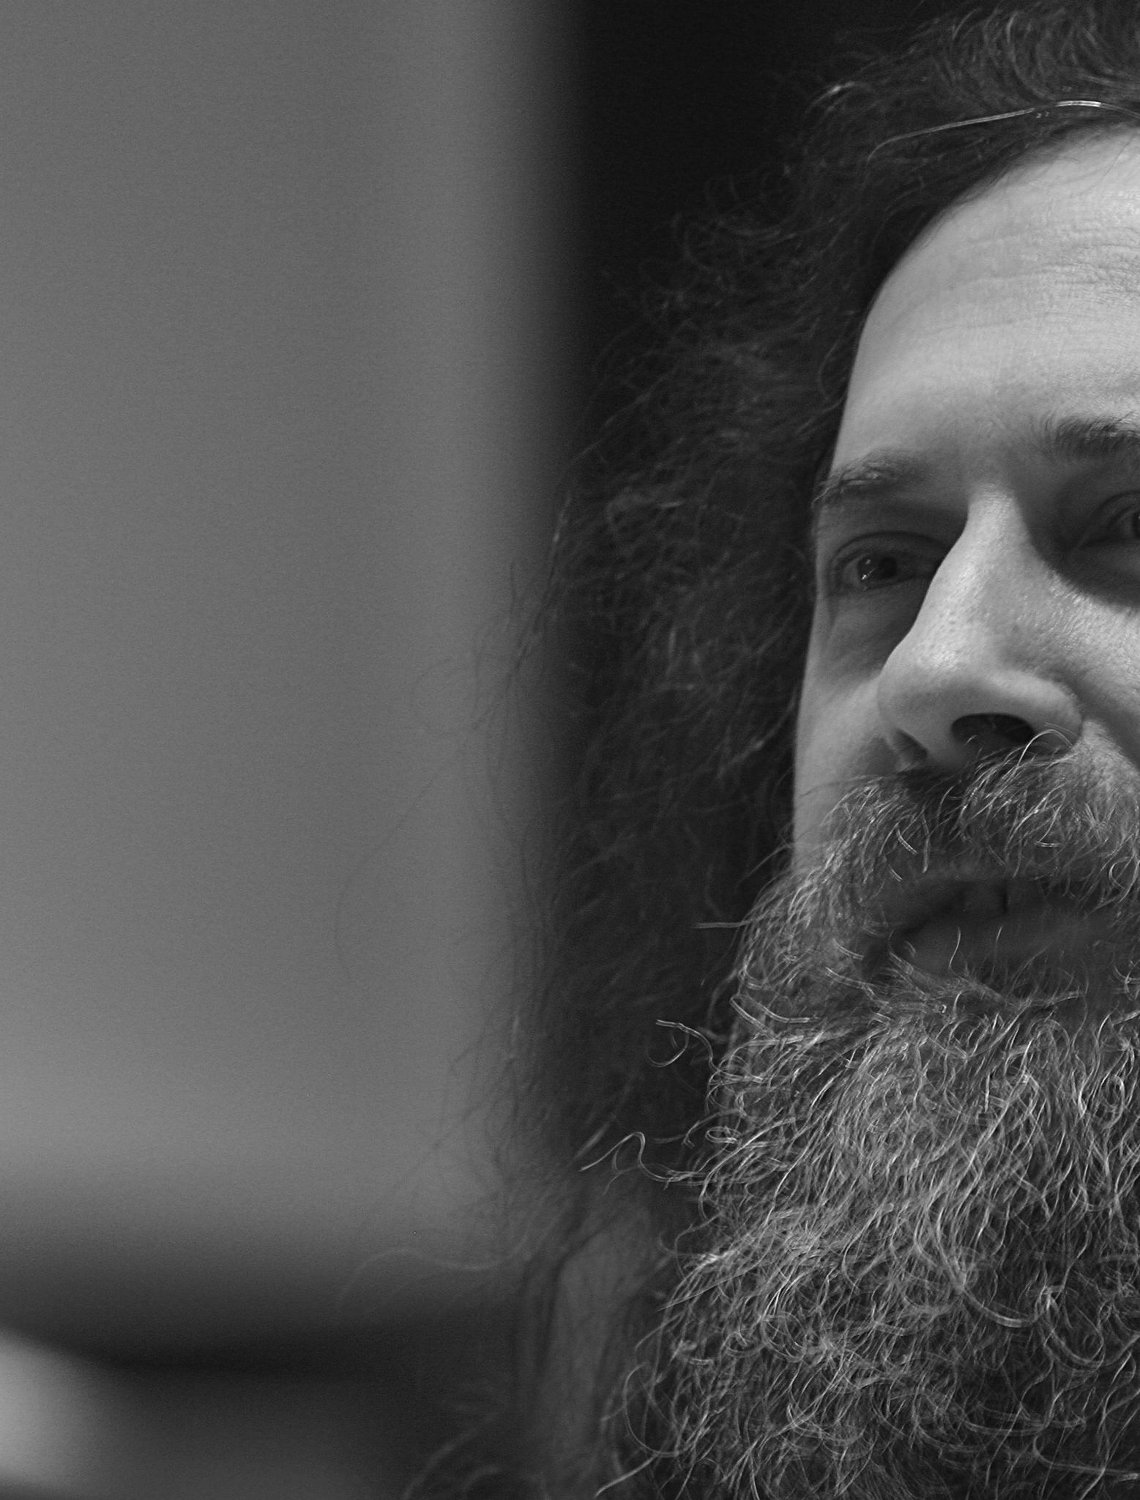
\includegraphics[width=\textwidth]{rms.jpg}
			\end{textblock}
		\else
			\begin{textblock}{11}(-8,0)
				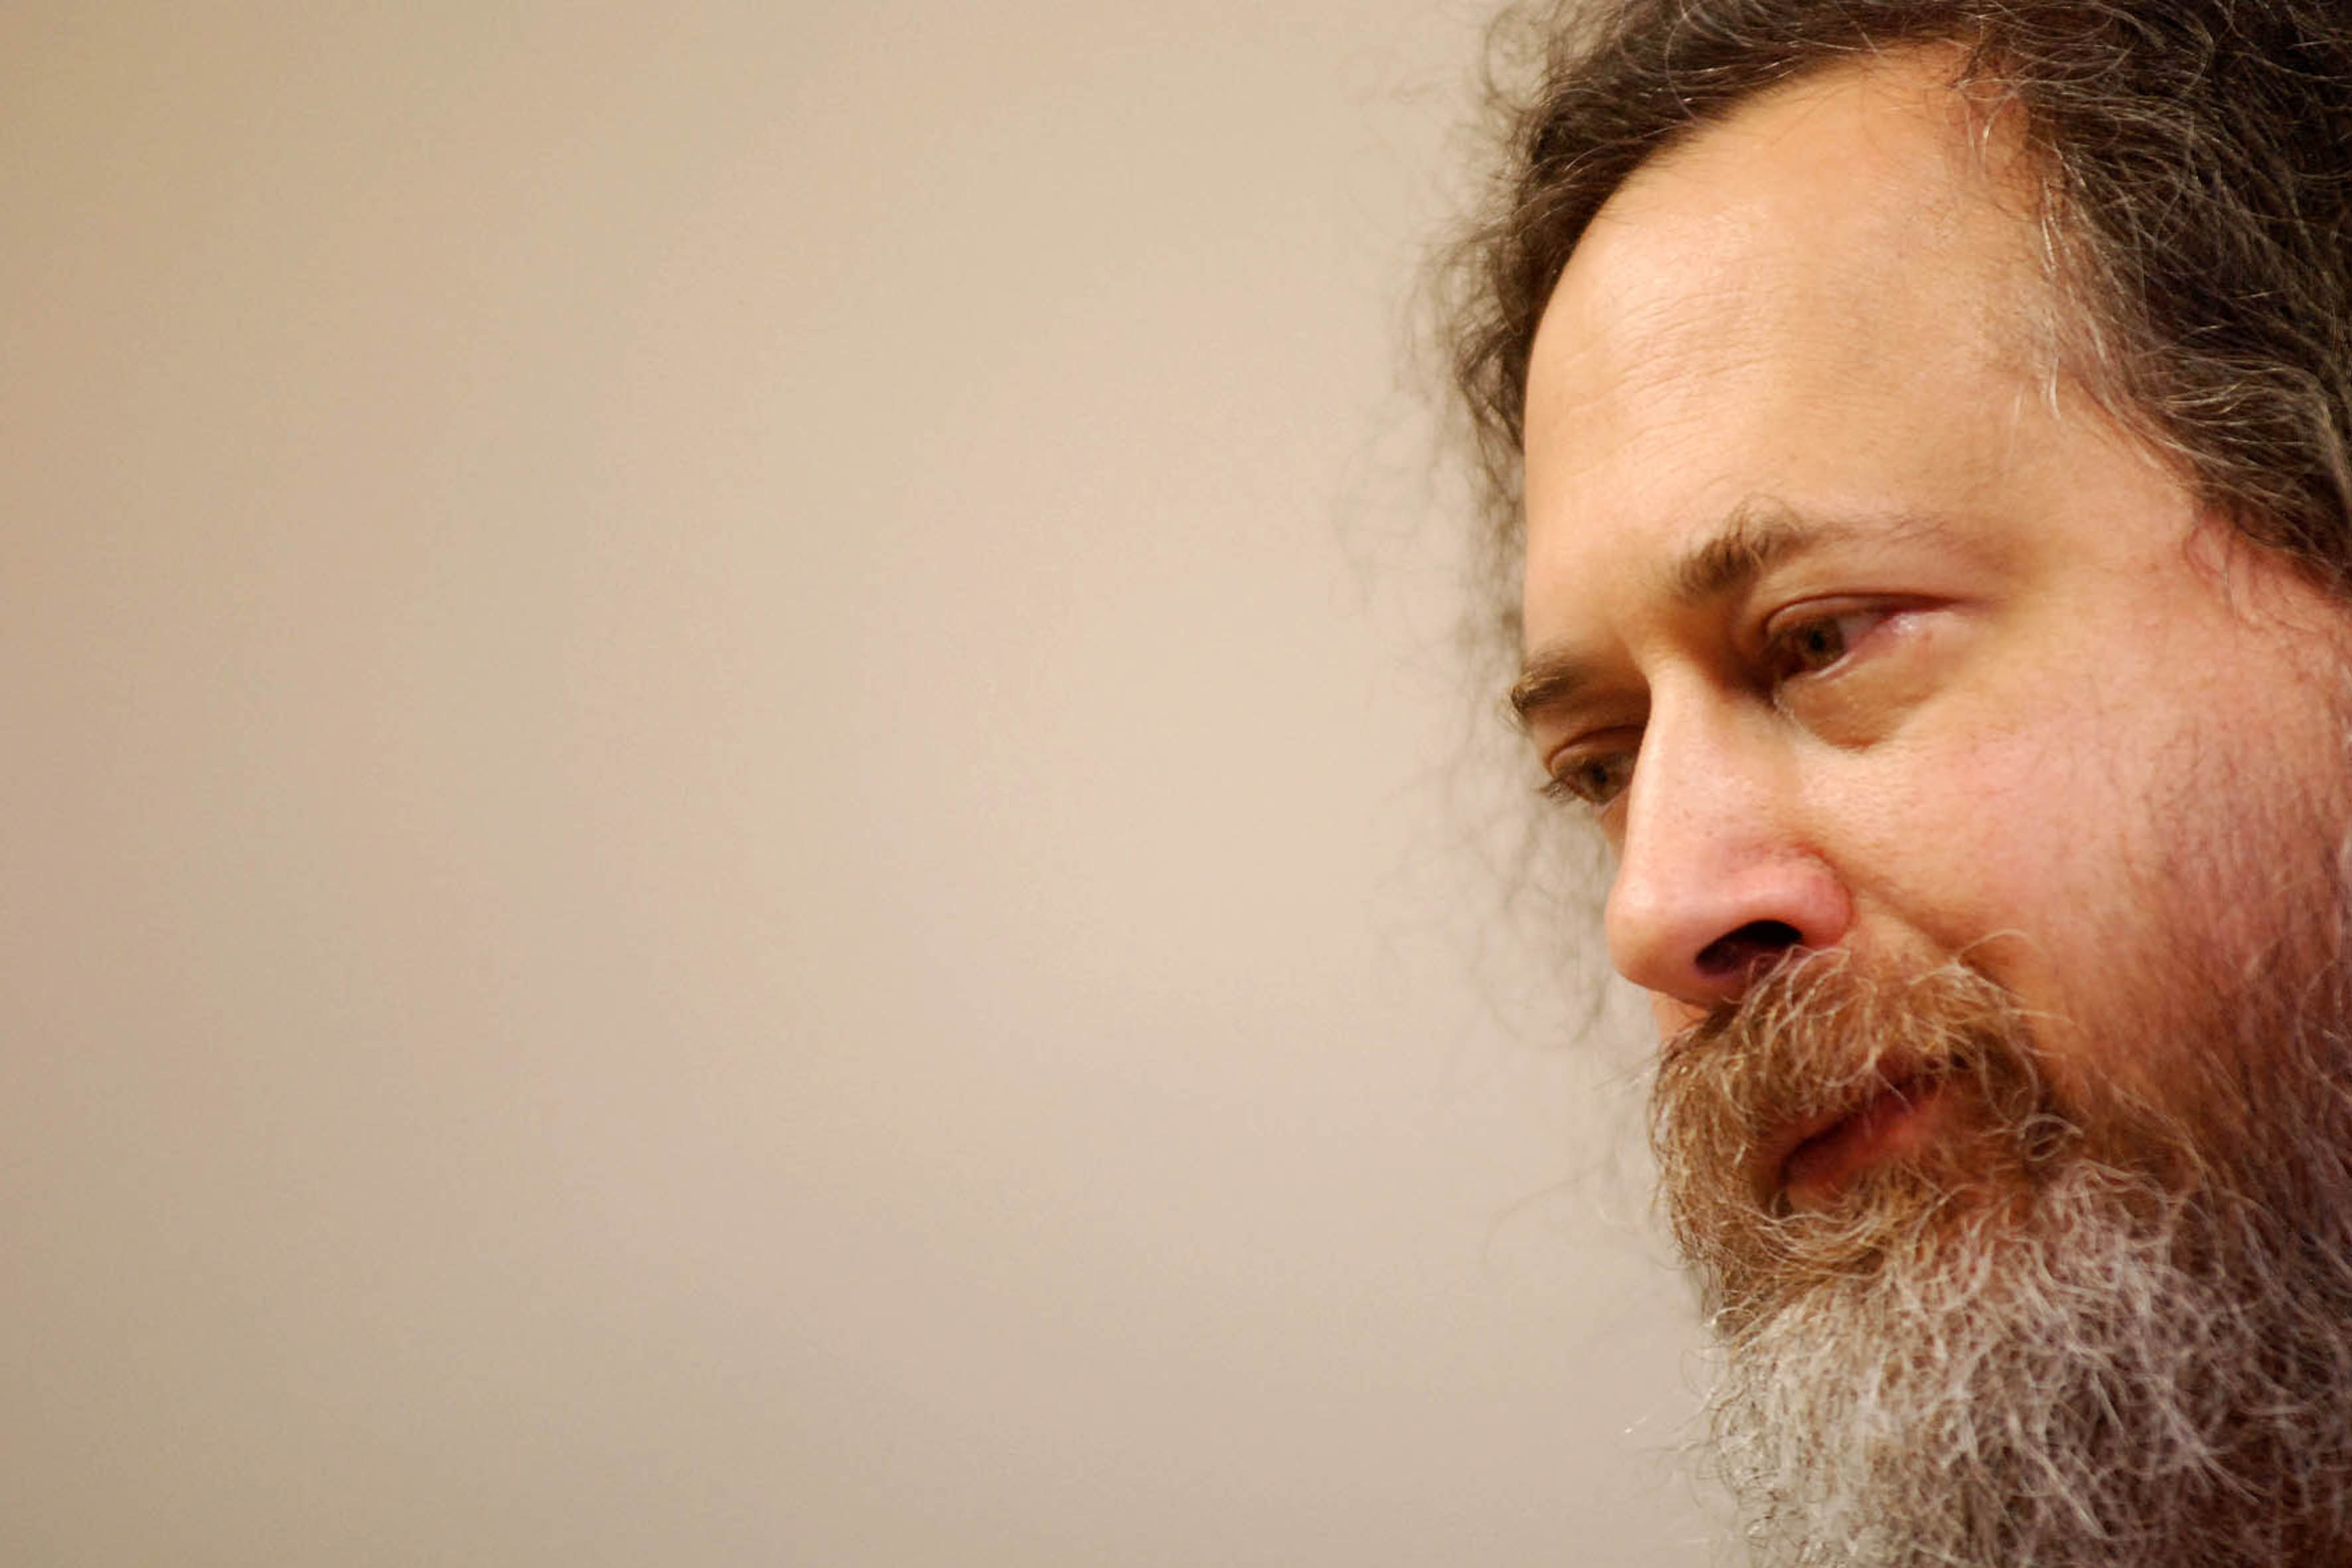
\includegraphics[height=1.3\textwidth]{nqn_richard_stallman.jpg}
			\end{textblock}
		\fi
		
		\vspace*{\fill}

		\changefont{phv}{m}{n}
		\vspace*{\fill}
		{\fontsize{42}{50}\selectfont	
			\textbf{Frei\vspace*{.2em}\\wie in\vspace*{.2em}\\ Freiheit\vspace*{.2em}\\}
		}
		{\large Richard Stallmans Kreuzzug\vspace*{.2em}\\ für freie Software\\~\\~}
%		\vspace*{\fill}
	
	    {\large Sam Williams\vspace*{.2em}\\ Revision: Richard M. Stallman\vspace*{.2em}\\ Übersetzung: Theo Walm}
	\end{titlepage}
\fi

\frontmatter
	Copyright \copyright{} 2002, 2010 Sam Williams\\
Copyright \copyright{} 2010 Richard M. Stallman\\
2011, 2012 Theo Walm

Permission is granted to copy, distribute and/or modify
this document under the terms of the GNU Free Documentation License,
Version 1.3 or any later version published by the Free Software
Foundation; with no Invariant Sections, no Front-Cover Texts, and no
Back-Cover Texts. A copy of the license is included in the section
entitled "`GNU Free Documentation License"'.

\comment{
	\bigskip

	Published by the Free Software Foundation\\
	51 Franklin St., Fifth Floor\\
	Boston, MA 02110-1335\\
	USA\\
	ISBN: 9780983159216\\
}
\bigskip

\ifnum\commercial=1
	Das Titelbild basiert auf einem flickr-Photo von \href{http://www.flickr.com/photos/redjar/474652905/}{redjar} und steht unter der Creative-Commons-Lizenz Attribution-ShareAlike 2.0 Generic (CC BY-SA 2.0).
\else
Das Titelbild stammt von Matías Subat und darf in Verbindung mit diesem Werk nichtkommerziell genutzt werden.
\fi

Das Photo der PDP-10 in Kapitel 7 stammt von Rodney Brooks. Das Photo von St. IGNUcius in Kapitel 8 stammt von Stian Eikeland. 

\subsection*{Abstammungshistorie}
\begin{itemize}
\item
\textit{Free as in Freedom: Richard Stallman's Crusade for Free Software}, 2002, Sam Williams, erschienen bei O'Reilly

\item
\textit{Free as in Freedom 2.0: Richard Stallman and the Free Software Revolution}, 2010, Richard Stallman, Sam Williams, erschienen bei GNU Press, \LaTeX-Quellcode unter \url{http://www.fsf.org/faif}

\item
\textit{Frei wie in Freiheit - Richard Stallmans Kreuzzug für freie Software, 2011, Theo Walm}, \LaTeX-Quellcode unter \url{http://github.com/yadayada/faif}

\end{itemize}

Die deutsche Ausgabe ist um das Vorwort und das Nachwort von Sam Willams sowie das Kapitel "`A Brief Journey through Hacker Hell"' gekürzt.

\subsection*{Danksagung}

Vielen Dank an Christian Mantey für die eingesandten Hinweise auf die Textfehler.

	\phantomsection
	\tableofcontents

	\addchap{Vorwort von Richard M. Stallman}


Ich habe versucht, in dieser Ausgabe mein Wissen mit den Gesprächen mit Williams und der Sichtweise von außen zu vereinen. Der geneigte Leser muss entscheiden, inwieweit mir das gelungen ist.

Ich habe den veröffentlichten Text der englischen Ausgabe erstmals 2009 gelesen, als ich um Mithilfe bei der französischen Übersetzung von \textit{Free as in Freedom} gebeten wurde. Es waren mehr als nur kleine Änderungen nötig. Viele Fakten mussten korrigiert werden, aber auch grundlegende Änderungen waren erforderlich. Williams als Nichtprogrammierer verwischte fundamentale technische und rechtliche Unterschiede wie das Verändern des Codes eines bestehenden Programms und das Implementieren einiger Ideen des Programms in einem anderen. So steht beispielsweise in der ersten Ausgabe, Gosmacs und GNU Emacs wären beide Modifikationen des ursprünglichen PDP-10-Emacs gewesen, was sie aber nicht sind. Weiterhin ist Linux fälschlicherweise als "`Version von Minix"' bezeichnet worden. SCO sollte später dieselbe Behauptung aufstellen, in ihrem berüchtigten Gerichtsverfahren gegen IBM; und Torvalds und Tanenbaum haben sie gemeinsam widerlegt. 

Die erste Ausgabe hat viele Ereignisse übertrieben dramatisch dargestellt, indem sie mit scheinbaren Emotionen verbunden wurden. 

Zum Beispiel stand geschrieben, ich habe 1992 "`Linux fast ignoriert"' und dann 1993 mit der Entscheidung, Debian GNU/Linux zu unterstützen, "`eine dramatische Kehrtwendung"' gemacht. Mein Interesse 1993 und mein Desinteresse 1992 waren Ausdruck derselben pragmatischen Vorgehensweise, die das Ziel verfolgte, das GNU-System zu vervollständigen. 
Der Start des GNU-Hurd-Kernels 1990 war ebensoein pragmatischer Schritt in diese Richtung.

Aus all diesen Gründen sind viele Aussagen in der Originalausgabe irrig oder stehen im falschen Zusammenhang. Es war notwendig, sie zu korrigieren, aber nicht direkt durch eine vollständige Überarbeitung, die aus anderen Gründen nicht wünschenswert war. Mir wurde vorgeschlagen, ausführliche Kommentare zu machen, aber in den meisten Kapiteln war das Ausmaß der Änderungen zu groß, um sie als Anmerkungen auszuführen. Einige Fehler waren zu tiefgehend oder verbreitet, um sie durch eine bloße Anmerkung richtigzustellen. Ergänzende Kommentare oder Fußnoten im Rest des Textes hätten das Textbild belastet und den Text schwer lesbar gemacht; Fußnoten wären von einigen Lesern übersprungen worden.
 
Ich habe deshalb die Korrekturen direkt im Text vorgenommen. Jedoch habe ich nicht alle Fakten und Zitate überprüft, die außerhalb meiner Expertise liegen; die meisten von ihnen habe ich auf Williams' Verantwortung so belassen. Williams’ Version enthielt viele Zitate, die kritisch meiner Person gegenüber sind. Diese habe ich alle nicht angetastet, nur bei Gelegenheit Gegendarstellungen angefügt. Ich habe keine Zitate entfernt, außer einige in Kapitel 11 über Open Source, die nichts mit meinem Leben oder Schaffen zu tun haben. Ebenso habe ich die meisten von Williams’ eigenen Interpretationen, die mich kritisieren, erhalten (und manche kommentiert), wenn sie keine falschen Auffassungen von Fakten oder über Technik enthielten. Aber ich habe die unzutreffenden Behauptungen zu meiner Arbeit und meinen Gedanken und Gefühlen frei berichtigt. Ich habe seine persönlichen Eindrücke beibehalten, wenn sie als solche dargestellt waren, und das "`ich"' im Text dieser Ausgabe bezieht sich auch immer auf Williams, ausgenommen bei den Anmerkungen, die mit "`RMS:"' eingeleitet werden.

In dieser Ausgabe ist das komplette System, das GNU und Linux umfasst, immer "`GNU/Linux"', und "`Linux"' allein bezieht sich auf Torvalds’ Kernel, ausgenommen in Zitaten, wo diese Verwendung des Begriffs mit "`[\textit{sic}]"' markiert wird. Siehe \url{http://www.gnu.org/gnu/gnu-linux-faq.html} für eine Erklärung, warum es falsch und ungerecht ist, das ganze System "`Linux"' zu nennen. 

Außerdem möchte ich John Sullivan für seine vielen nützlichen kritischen Gedanken und seine Vorschläge danken.

	%\include{vorwort_wil}

\mainmatter
	%\chapter{Es war einmal ein Drucker}
\chapter{Am Anfang war der Drucker}
\pagenumbering{arabic}

\begin{quotation}
Ich fürchte die Danaer, auch wenn sie Geschenke bringen.

- Vergils \textit{Aeneid}
\end{quotation}

% TODO: Jahreszahl herausfinden
\comment{Das AI Lab und das Laboratory for Computer Science wurden 2003 zum CSAIL zusammengelegt.}

Der neue Drucker hatte schon wieder einen Papierstau.
Richard M. Stallman, angestellter Programmierer am Artificial Intelligence Laboratory (AI~Lab) des Massachusetts Institute of Technology, sollte es noch herausfinden. 

Eine Stunde, nachdem er eine 50seitige Datei an den Laserdrucker geschickt hatte, unterbrach Stallman, 27, seine Arbeit, um sein Dokument holen zu gehen. Bei der Ankunft lagen nur vier Seiten in der Papierausgabe. Und dazu kam, dass die vier Seiten nicht einmal zu seiner gedruckten Datei gehörten. Stallmans und der Rest des Druckauftrags eines anderen waren immer noch in der Kabelage des Netzwerks gefangen.

Auf Geräte warten zu müssen ist ein Berufsrisiko, wenn man Programmierer ist, also nahm Stallman es hin. Trotzdem ist der Unterschied zwischen dem Warten auf ein Gerät und dem Warten an einem Gerät ein beträchtlicher. Es war nicht das erste Mal, dass er am Drucker stehen und den Ausdruck jeder einzelnen Seite überwachen musste. Als jemand, der den Großteil seiner Tage und Nächte damit verbringt, die Leistung von Geräten und die sie steuernde Software zu verbessern, fühlte Stallman den Drang, das Gerät zu öffnen, sich seine Innereien anzusehen und das Übel an seiner Wurzel zu packen.

Leider erstreckten sich Stallmans programmiererische Fähigkeiten nicht in den Bereich des Maschinenbaus. Während frische Ausdrucke aus dem Gerät schossen, hatte Stallman Gelegenheit, über Wege nachzudenken, wie man das Papierstauproblem lösen konnte. 

Wie lange war es her gewesen, dass die Angestellten des AI Labs den neuen Drucker in Empfang genommen hatten, fragte sich Stallman. Das Gerät war eine Schenkung der Xerox Corporation. Ein innovativer Prototyp, ein umgebauter Xerox-Photokopierer. Anstatt physisch Kopien zu machen, empfing er Daten über das Netzwerk und verwandelte sie in professionell aussehende Dokumente. Er war von den Ingenieuren in Xerox' weltbekannter Forschungseinrichtung in Palo Alto (PARC) entworfen worden, und war einfach gesagt ein Vorgeschmack auf die Revolution des Desktop-Printings, die den Rest der Computerindustrie Ende des Dezenniums erfassen würde.

%alter Druckertyp aus einem Interview in "Making It Big in Software"
Getrieben vom instinktiven Drang, an der neuen Technik herumzuspielen, hatten die Programmierer am AI~Lab das neue Gerät prompt in die ausgeklügelte Computerinfrastruktur integriert. Die Ergebnisse waren sofort zufriedenstellend. Der neue Xerox-Drucker war schnell, ganz im Gegensatz zum alten Labordrucker, einem XeroGraphic Printer. Die Seiten kamen im Sekundentakt aus dem Drucker, wodurch ein ehemals 20minütiger Druckauftrag nur noch 2 Minuten dauerte. Das neue Gerät war außerdem präziser. Ausgedruckte Kreise sahen auch so aus wie Kreise und nicht oval; gerade Linien waren gerade Linien, keine flachen Sinusschwingungen.

Er war, alles in allem, ein zu gutes Geschenk, um ihn auszuschlagen.

Als das Gerät dann im Einsatz war, kamen seine Mängel zum Vorschein. Der größte Nachteil war seine Anfälligkeit für Papierstaus. Die technisch denkenden Programmierer verstanden schnell den Grund hinter diesem Fehler. Als Photokopierer bedurfte das Gerät generell die Überwachung durch einen Bediener. Unter der Annahme, diese Bediener wären immer vor Ort, um Papierstaus zu beheben, falls einer auftritt, widmeten die Ingenieure bei Xerox ihre Zeit der Behebung anderer Probleme.\comment{In der engineering terms, user diligence was builtinto the system.}

Durch die Wandlung des Geräts in einen  Drucker hatten die Ingenieure bei Xerox die Mensch-Maschine-Beziehung auf eine subtile, aber profunde Art verändert. Statt einem einzelnen menschlichen Bediener zu gehorchen, war er nun Knecht aller Benutzer im gesamten Netzwerk. Statt direkt am Gerät zu stehen, schickte nun ein Benutzer am einen Ende des Netzwerks seinen Druckauftrag über eine Eimerkette aus Rechnern und erwartete, dass die gewünschten Daten an der richtigen Stelle in korrekter Form eintreffen.\comment{Erst wenn jemand schließlich das Resultat holen wollte, würde er merken, wie wenig wirklich gedruckt wurde.}

Stallman war wohl kaum der einzige Bewohner des AI~Labs, der das Problem erkannte, aber er dachte auch an eine Abhilfe. Jahre zuvor hatte Stallman ein ähnliches Problem bei dem alten Drucker behoben, indem er die Software auf einer kleinen PDP-11 abänderte, die den Drucker gesteuert hat, und das Incompatible Timesharing System, das auf dem PDP-10-Hauptrechner lief. Stallman konnte die Papierstaus nicht verhindern, aber er konnte Code schreiben, mit dem die PDP-11 den Drucker regelmäßig abfragt und der den Papierstau an die PDP-10 meldet. Stallman schrieb außerdem Code für die PDP-10, der jedem Nutzer mit einem ausstehenden Druckauftrag eine Nachricht schickt, dass der Drucker Papierstau hat. Die Nachricht war simpel, in etwa "`Der Drucker ist verklemmt, bitte beheben."' Und weil sie an die Leute geschickt wurde, die das größte Interesse daran hatten, das Problem zu beheben, standen die Chancen nicht schlecht, dass das Problem alsbald aus der Welt geschafft würde.

Stallmans Fehlerkorrektur war – wie sie es nun einmal an sich haben – indirekt, aber elegant. Sie brachte den mechanischen Fehlstand nicht wieder in Ordnung, aber durchbrach zumindest die Informationsbarriere zwischen Benutzer und Gerät. Dank einiger Zeilen Code konnten die AI-Lab-Angestellten sich die 10 bis 15 Minuten jede Woche mit dem Hin- und Herlaufen zum Prüfen des Druckers sparen. 
Stallmans Fehlerbehebung nutzte die kollektive Intelligenz des Netzwerks aus. "`Wenn man die Nachricht bekommen hat, konnte man nicht davon ausgehen, dass jemand anders sich darum kümmern würde"', erinnert sich Stallman an die Logik dahinter. "`Man musste zum Drucker gehen. Ein, zwei Minuten, nachdem der Drucker Schwierigkeiten machte, standen zwei, drei Leute, die die Nachricht bekommen hatten, am Drucker, um den Stau zu beheben. Von den zwei oder drei Leuten wusste meist mindestens einer, wie man das Problem behebt."'

Solche cleveren Fehlerausbügelungen waren ein Markenzeichen des AI Labs und seiner Ureinwohnerschaft aus Programmierern. Allerdings lehnten die besten Programmierer am AI~Lab den Begriff "`Programmierer"' ab und bevorzugten stattdessen die saloppe Berufsbezeichnung "`Hacker"'. Die Bezeichnung deckte eine Fülle an Tätigkeiten ab – vom kreativen Klamauk bis hin zur Verbesserung bestehender Software und Computersysteme. In der Bezeichnung schwingt auch etwas von einer Yankee-Bauernschläue mit.
Für einen Hacker ist das Schreiben von funktionierender Software nur der Anfang. Ein Hacker würde versuchen, seine eigene Finesse zum Ausdruck zu bringen (und andere Hacker zu beeindrucken), indem er eine zusätzliche Herausforderung angeht: das Programm besonders schnell, klein, mächtig, elegant oder eindrucksvoll zu machen.\footnote{Mehr zum Begriff "`Hacker"' gibt es im \nameref{Anhang A}.}

Bei Unternehmen wie Xerox war es gängige Praxis, ihre Produkte (und Software) an Institutionen zu verschenken, an denen Hacker zusammenkommen. Wenn Hacker ihre Produkte nutzten, würden sie vielleicht später für ihr Unternehmen arbeiten. In den 60ern und 70ern entwickelten sie auch gelegentlich Programme, die nützlich für den Hersteller waren und an andere Kunden ausgeliefert werden konnten. 

Als Stallman beim Xerox-Laserdrucker die Neigung zu Papierstaus bemerkte, dachte er daran, die alte Fehlerkorrektur – den "`Hack"' – bei ihm anzuwenden. Als er sich jedoch in Folge die Druckersoftware ansehen wollte, machte Stallman eine unschöne Entdeckung. Es gab für den Drucker keine Software, oder jedenfalls keine, die Stallman oder einer seiner Kollegen lesen konnte. Bis dahin gehörte es für die meisten Firmen zum guten Ton, ihre Quellcodedateien zu veröffentlichten, lesbare Textdateien, die die einzelnen Maschinenbefehle dokumentieren. Xerox hatte in diesem Fall nur die Software in kompilierter, also Binärform ausgeliefert. Wenn sich ein Programmierer diese Dateien ansieht, sieht er nur endlose Kolonnen aus Nullen und Einsen, chinesisch.

Es gibt Programme, sogenannte "`Disassembler"', die die Nullen und Einsen in maschinennahe Befehle übersetzen, aber herauszufinden, was diese Befehle nun  wirklich "`tun"', ist eine langwierige und komplizierte Aufgabe, bekannt als "`Reverse engineering"'. Dieses Programm zu reverse-engineeren, hätte gut mehr Zeitaufwand benötigt als 5 Jahre Drucken mit gelegentlichen Papierstaus. So frustriert war Stallman nicht deswegen und tat das Problem ab. 

Xerox' unfreundliche Firmenpolitik stand im krassen Gegensatz zu den üblichen Gepflogenheiten in der Hackergemeinschaft. Zum Beispiel brauchte das AI~Lab zur Entwicklung des Programms für die PDP-11, die den alten Drucker steuerte, und des Programms für eine andere PDP-11, die die Bildschirmterminals handhabt, zum Bauen der PDP-11-Programme auf dem PDP-10-Hauptrechner einen Cross-Assembler. Die Hacker im Lab hätten einen schreiben können, aber Stallman, ein Harvard-Student, fand ein solches Programm auf einem Rechner im Computerlabor von Harvard. Das Programm war für den gleichen Rechnertyp geschrieben, die PDP-10, aber für ein anderes Betriebssystem. Stallman hat nie herausgefunden, wer das Programm geschrieben hatte, weil es nicht im Quellcode stand. Aber er brachte eine Kopie mit ins AI Lab. Er änderte den Quellcode, damit es auf dem Incompatible Timesharing System (ITS)\index{ITS|(} lief, das im AI~Lab eingesetzt wurde. Ohne große Schwierigkeiten konnte das AI~Lab so an das Programm gelangen, das es für seine Softwareinfrastruktur benötigte. Stallman fügte sogar einige neue Funktionen hinzu, die es in der Ursprungsversion nicht gab. "`Wir haben es letztendlich mehrere Jahre eingesetzt"', sagt Stallman.

Aus der Sicht eines Programmierers der 70er war dieser Vorgang nichts anderes als wie ein vorbeikommender Nachbar, der sich ein Elektrowerkzeug oder eine Tasse Zucker von einem borgt. Der einzige Unterschied war, dass Stallman mit dem Kopieren der Software für das AI~Lab keinem anderen die Nutzung des Programms unmöglich machte. Wenn überhaupt, profitierten andere Hacker von dem Vorgang, weil Stallman es um neue Funktionalität ergänzt hatte, die andere Hacker gerne rückübernehmen konnten. Stallman erinnert sich zum Beispiel an einen Programmierer einer privaten Firma, Bolt, Beranek \& Newman, der sich das Programm entlehnt hat. Er brachte es auf Twenex zum Laufen und erweiterte es um einige Funktionen, die Stallman wiederum schließlich in den AI-Lab-Quellcode eingepflegt hat. Zwei der Programmierer hatten sich entschlossen, zusammen eine gemeinsame Version zu verwalten, die auf ITS\index{ITS|)} und Twenex läuft.

"`Ein Programm entwickelte sich so, wie sich eine Stadt entwickelt"', sagt Stallman, wenn er sich an die Infrastruktur des AI~Labs erinnert. "`Einige Teile wurden ausgetauscht und erneuert. Neue Dinge wurden hinzugefügt. Aber man konnte sich immer einen bestimmten Teil ansehen und sagen, \glq Hmm, dem Stil nach wurde dieser Teil in den frühen 60ern geschrieben und dieser Teil Mitte der 70er.\grq\,"'

Mit diesem System der geistigen Akkumulierung erschufen die Hacker am AI~Lab und anderswo robuste Werke. Nicht jeder Programmierer, der an dieser Kultur teilhatte, bezeichnete sich selbst als Hacker, aber die meisten teilten die Ansichten Stallmans. Wenn ein Programm oder ein Patch die eigenen Probleme löst, warum sollte es dann nicht auch die der anderen lösen können. Warum sollte man nicht selbstlos mit anderen teilen?

Dieses Kooperationssystem wurde durch kommerzielle Geheimhaltung und Gier unterminiert, was zu seltsamen Kombinationen aus Geheimhaltung und Zusammenarbeit führte. Zum Beispiel hatten die Informatiker an der UC Berkeley ein mächtiges Betriebssystem namens BSD geschrieben, das auf dem Unix-System basierte, das sie von AT\&T erworben hatten. Berkeley stellte BSD für den Preis einer Kopie auf Band zur Verfügung, gab solche Bänder aber nur an Schulen heraus, die eine für 50.000\$ gekaufte Lizenz von AT\&T vorweisen konnten. Die Berkeley-Hacker stellten weiterhin alles soweit zur Verfügung, wie AT\&T es zuließ, aber sie erkannten keinen Konflikt zwischen diesen beiden Verhaltensweisen.

Ebenso störte es Stallman, dass Xerox den Quellcode nicht mitgeliefert hatte, aber er war noch nicht wütend. Er hatte nie daran gedacht, Xerox nach dem Quellcode zu fragen. "`Sie hatten uns schon den Laserdrucker geschenkt"', sagt Stallman. "`Sie waren uns nicht mehr schuldig. Außerdem bin ich davon ausgegangen, dass das Fehlen des Quellcodes Ausdruck einer wissentlichen Entscheidung war, und sie darum zu bitten aussichtslos gewesen wäre."' 

Aber schließlich gab es gute Nachrichten: gerüchteweise hieß es, dass ein Wissenschaftler an der Informatik-Fakultät der Carnegie Mellon University den Quellcode zum Laserdrucker hatte. Der Bezug zur Carnegie Mellon verhieß nichts Gutes. 1979 hatte Brian Reid\index{Reid, Brian}, Doktorand an dieser Universität, die Gemeinschaft brüskiert, als er sich weigerte, sein Textformatierungsprogramm Scribe\index{Scribe|(} offenzulegen. Seine Formatierungssprache war die erste, die Formatierungsbefehle hatte, die an der gewünschten Semantik orientiert waren (wie etwa "`dieses Wort hervorheben"' oder "`dieser Absatz ist ein Zitat"'), anstatt konkrete Formatierungsdetails zu verwenden ("`dieses Wort kursiv setzen"' oder "`die Ränder dieses Absatzes verschmälern"').
Reid verkaufte Scribe an Unilogic, ein Softwareunternehmen aus dem Raum Pittsburgh. Zum Ende seiner Zeit als Doktorand sagte Reid, er wollte einfach einen Weg finden, wie er das Programm an Programmierer übergeben konnte, ohne dass es in die Gemeinfreiheit rutscht. (Warum jemand einen solchen Ausgang als besonders unerwünscht ansehen sollte, bleibt unklar.) Dem ganzen setzte Reid noch das Sahnehäubchen auf, als er dem Einbau zeitgesteuerter Funktionen zustimmte – von Programmierern "`Zeitbomben"' genannt – die die Gratiskopien des Programms nach einem Verfallsfrist von 90 Tagen deaktivieren. Um die Deaktivierung zu verhindern, würden Nutzer das Softwareunternehmen bezahlen, das dann einen Schlüssel herausgab, der die interne Zeitbomben-Antifunktion entschärfen konnte.

Für Stallman was das schlichtweg Verrat am Programmiererethos. Statt die Idee des Teilens und Weitergebens zu ehren, hatte Reid einen Weg für Unternehmen geschaffen, Programmierern für den Zugang zu Informationen Geld abzunötigen. Aber er dachte damals nicht weiter über dieses Problem nach, weil er Scribe nur selten benutzte.

Unilogic stellte dem AI Lab eine Gratisversion zur Verfügung, ließ aber die Zeitbombe aktiviert und erwähnte sie mit keinem Wort. Die Software funktionierte eine Zeit lang; dann kam eines Tages ein Bericht von einem Nutzer, dass Scribe\index{Scribe|)} nicht mehr funktioniert. Der Hacker Howard Cannon verbrachte einige Stunden mit dem Debuggen der Binärdatei, bis er die Zeitbombe fand und patchte sie heraus. Cannon war empört und machte keinen Hehl daraus. Er erzählte anderen Hackern, wie sauer er war, dass Unilogic seine Zeit mit einem absichtlichen Bug verschwendet hatte.

Stallman besuchte aus beruflichen Gründen einige Monate später den Campus der Carnegie Mellon. Während seines Aufenthalts wollte er die Person ausfindig machen, die angeblich den Quellcode zu der Druckersoftware hatte. Wie der Zufall so spielte, war der Mann gerade in seinem Büro. In bester Ingenieursmanier war das Gespräch höflich, aber direkt. Nachdem er sich kurz als Besucher vom MIT vorgestellt hatte, fragte Stallman nach dem Quellcode für den Laserdrucker, den er ändern wollte. Zu seinem Ärger verweigerte der Forscher die Herausgabe. "`Er sagte mir, er hätte versprochen, mir keine Kopie zu geben"', so Stallman. 

Das Gedächtnis ist ein seltsames Sieb\comment{seltsam' Ding}. Zwanzig Jahre nach dem Ereignis ist Stallmans geistiges Magnetband von dieser Erinnerung stellenweise leer. Nicht nur kann er sich nicht mehr an den Zweck der Reise entsinnen, oder die Jahreszeit, zu der er sie antrat, sondern kann sich auch nicht mehr erinnern, mit wem er das Gespräch geführt hat. Laut Reid ist derjenige, mit dem Stallman am wahrscheinlichsten zu tun hatte, Robert Sproull\index{Sproull, Robert}, ehemaliger Forscher am Xerox PARC und derzeitiger Leiter der Oracle Laboratories, einer Forschungsabteilung des Konglomerats Oracle Corporation. In den 70ern war Sproull der Hauptentwickler der besagten Laserdruckersoftware, als er am Xerox PARC arbeitete. Um 1980 nahm Sproull eine Forschungsstelle an der Carnegie Mellon an, wo er seine Arbeit rund um Laserdrucker fortsetzte und anderen Projekten nachging.

Wenn man ihn direkt danach fragt, kann sich Sproull nicht erinnern. "`Ich kann keine sachliche Aussage machen"', schreibt Sproull via E"~Mail. "`Ich kann mich an diesen Vorfall nicht im Geringsten erinnern."' "`Der Code, den Stallman wollte, war innovativer, modernster Code, den Sproull etwa im Jahr, bevor er an die Carnegie Mellon ging, geschrieben hatte"', erinnert sich Reid. Falls das der Fall ist, könnte daraus ein Missverständnis erwachsen sein, weil Stallman den Quellcode für ein Programm wollte, das das MIT schon längere Zeit einsetzte, und nicht die neuere Version. Aber die Frage, um welche Version es sich handelt, kam in dem kurzen Gespräch nicht auf.

In seinen Vorträgen vor Publikum hat Stallman oft von diesem Vorfall berichtet und erwähnt, dass die Weigerung, den Quellcode auszuhändigen, von einer Geheimhaltungserklärung herrührt, einem Vertrag zwischen jener Person und der Xerox Corporation, die dem Unterzeichner Zugang zum Quellcode ermöglicht, wenn er sich verpflichtet, ihn vertraulich zu behandeln. In der heutigen Zeit ist die Geheimhaltungserklärung (NDA) ein Standardinstrument in der Softwareindustrie; damals war sie ein Novum, ein Ausdruck des kommerziellen Werts des Laserdruckers und der Informationen über seine Funktionsweise für Xerox. "`Xerox hatte zu der Zeit versucht, ein kommerzielles Produkt aus dem Laserdrucker zu machen"', erinnert sich Reid. "`Sie wären verrückt gewesen, wenn sie den Quellcode herausgegeben hätten."'

Für Stallman jedoch stellte sich die Geheimhaltungserklärung ganz anders dar – als Weigerung eines CMU-Forschers, der Gemeinschaft beizutragen, die bis dahin Programmierer ermutigt hatte, Software als Gemeingut anzusehen. Wie ein Kleinbauer, dessen jahrhundertealter Bewässerungsgraben plötzlich ausgetrocknet war, war Stallman dem Verlauf des Grabens zu seinem Ursprung gefolgt, und fand dort einen brandneuen Staudamm vor, auf dem das Xerox-Logo prangte.

Für Stallman brauchte die Erkenntnis, dass Xerox einen Programmiererkollegen genötigt hatte, an diesem neumodischen System erzwungener Geheimhaltung teilzunehmen, eine Weile zum Sacken. Im ersten Moment konnte er die Weigerung nur auf sich persönlich beziehen. "`Ich war so wütend, dass ich nicht wusste, wie ich mich ausdrücken sollte. Also habe ich mich einfach umgedreht und bin ohne ein Wort gegangen"', erinnert sich Stallman. "`Vielleicht habe ich die Tür zugeschlagen, wer weiß. Ich kann mich bloß noch erinnern, dass ich nur noch weg wollte. Ich bin in sein Büro gekommen, weil ich davon ausgegangen bin, dass er hilft. Ich hatte nicht darüber nachgedacht, wie ich reagieren sollte, wenn er sich weigert. Als er das dann tat, war ich fassungs- und sprachlos und auch enttäuscht und wütend."' 

Zwanzig Jahre danach hält die Wut noch an und Stallman stellt den Vorfall als einen dar, der ihn das ethische Problem hat angehen lassen, aber nicht als den einzigen. In den folgenden Monaten sollte sich Stallman und der Hackergemeinde des AI~Labs eine Reihe an Ereignissen widerfahren, die die 30 Sekunden Spannung in dem fernen Büro an der Carnegie Mellon in den Schatten stellen würden. Wenn es jedoch darum geht, der Reihe an Ereignissen nachzugehen, die den solitären Hacker Stallman mit seinem instinkiven Misstrauen gegen zentrale Autorität zu dem kreuzzüglerhaften Aktivisten gemacht haben, der für die traditionellen Werte der Freiheit, Gleichheit und Brüderlichkeit in der Welt der Softwareentwicklung einsteht, schenkt Stallman dem Carnegie-Mellon-Vorfall besondere Aufmerksamkeit.
"`Es war meine erste Begegnung mit einer Geheimhaltungserklärung und sie hat mich gelehrt, dass es dabei Opfer gibt"', sagt Stallman mit Nachdruck. "`In dem Fall war ich das Opfer. [Das Lab und ich] waren die Opfer."'

Stallman erklärt später: "`Wenn er mir aus persönlichen Gründen seine Zusammenarbeit verwehrt hätte, wäre es kein größeres Problem gewesen. Ich hätte ihn vielleicht für einen Drecksack gehalten, mehr nicht. Der Umstand, dass die Weigerung nichts mit mir zu tun hatte, dass er im Vorhinein versprochen hatte, unsozial zu sein, nicht nur mir gegenüber, sondern gegen jeden, hat das Ganze zu einem wichtigen Thema werden lassen."'

Obwohl schon frühere Ereignisse Stallmans Geduld auf die Probe gestellt hatten, sagt er, bis zum Vorfall an der Carnegie Mellon war ihm nicht bewusst gewesen, dass diese Vorgänge anfingen, in eine Kultur einzudringen, die er lange als heilig angesehen hatte. Er sagte, "`Ich hatte schon die Vorstellung, dass Software ausgetauscht werden sollte, war mir aber nicht sicher, wie ich darüber denken sollte. Meine Gedanken waren unklar und unorganisiert, so dass ich sie nicht in einer präzisen Form der Welt hätte mitteilen können. Nach dieser Erfahrung fing ich an, zu erkennen, was das Problem und wie bedeutend es war."'

Als Eliteprogrammierer an einer Eliteeinrichtung war Stallman ohne Weiteres bereit gewesen, die Kompromisse und Kuhhandel zu ignorieren, die seine Programmiererkollegen eingingen, solange sie nicht seine eigene Arbeit behinderten. Bis zur Anlieferung des Xerox-Laserdruckers hatte Stallman sich damit zufriedengegeben, auf die Geräte und Programme herabzusehen, die andere Nutzer grimmig tolerierten.

Nun, da sich der Laserdrucker ins Netzwerk des AI Lab eingeschlichen hatte, hatte sich etwas geändert. Das Gerät funktionierte gut, abgesehen von den Papierstaus. Aber die Möglichkeit, die Software nach dem persönlichen Geschmack oder zum Nutzen der Allgemeinheit abzuändern, war ihnen genommen. Aus der Sicht der Softwareindustrie stellte die Druckersoftware eine Änderung in der Geschäftsstrategie dar. Software war ein so wertvolles Gut geworden, dass Unternehmen nicht länger die Notwendigkeit sahen, den Quellcode zu veröffentlichen, besonders wenn die Veröffentlichung potentiellen Konkurrenten die Möglichkeit einer billigen Nachahmung eröffnete. Aus Stallmans Sicht war der Drucker ein trojanisches Pferd. Nach einem Jahrzehnt des Misserfolgs sollte Software, die der Nutzer nicht verändern und weitergeben kann – in Zukunft würden Hacker sie "`proprietäre Software"' nennen – durch gewiefte Methoden im AI~Lab Fuß gefasst haben. Sie kam in der Gestalt eines Geschenks.

Dass Xerox einigen Programmierern Zugang zu weiteren Geschenken in Gegenleistung zur Geheimhaltung angeboten hat, war ebenso ärgerlich, aber Stallman merkt an\comment{takes pains to note that}, dass wenn ihm in jüngeren Jahren so ein Quid-pro-quo-Handel angeboten worden wäre, er ihn vielleicht angenommen hätte. Aber der Ärger mit dem Vorfall an der Carnegie Mellon hatte einen festigenden Effekt auf Stallmans eigene moralische Farblosigkeit. Nicht nur verhalf er ihm zu dem Zorn, zukünftig solche Angebote skeptisch zu sehen, er zwang ihn auch, die ganze Sache umzudrehen: Was, wenn ein Hackerkollege eines Tages in sein Büro kommen sollte und es nun Stallmans Aufgabe wäre, ihm den Quellcode vorzuenthalten?
"`Als mir jemand angeboten hat, all meine Kollegen auf diese Art zu verraten, habe ich mich daran erinnert, wie ärgerlich ich war, als man mit mir und dem ganzen Lab dasselbe gemacht hat"', sagt Stallman. "`Also hab ich gesagt \glq Vielen Dank, dass Sie mir dieses schöne Softwarepaket angeboten haben, aber ich kann es unter den Bedingungen, die Sie verlangen, nicht annehmen und muss wohl ohne es auskommen.\grq\,"'

Es war eine Lektion, die Stallman in den turbulenten 80er Jahren bleiben sollte, einem Jahrzehnt, in dem viele seiner MIT-Kollegen vom AI~Lab gehen und selbst Geheimhaltungserklärungen unterschreiben sollten. Sie haben vielleicht bei sich gedacht, dass das ein notwendiges Übel ist, um das Beste für ihre Projekte zu erreichen. Aber für Stallman zog es die moralische Rechtmäßigkeit der Projekte in Frage. Wozu soll ein spannendes technisches Projekt gut sein, wenn es der Gemeinschaft vorenthalten werden soll?

Stallman sollte bald lernen, dass das Ausschlagen solcher Angebote mehr als nur persönliche Opfer erforderte. Es erforderte die Absonderung von seinen Hackerkollegen, die zwar auch eine ähnliche Abneigung gegenüber Geheimhaltung hatten, sie aber in einer moralisch flexibleren Art ausdrückten. Jemandem die Herausgabe des Quellcodes zu verweigern, entschied sich Stallman, war nicht nur ein Verrat am wissenschaftlichen Auftrag, der die Softwareentwicklung seit dem Ende des Zweiten Weltkriegs gefördert hatte, sondern es war die Verletzung der Goldenen Regel, dem moralischen Grundsatz, andere so zu behandeln, wie man selbst behandelt werden will.

Daher rührt die Bedeutsamkeit des Laserdruckers und der Begegnung, die sich seinetwegen ergab. Ohne ihn, sagt Stallman, hätte sein Leben vielleicht einen gewöhnlicheren Verlauf genommen, ein Leben, in dem er mit den materiellen Vorzügen als kommerzieller Programmierer seine Frustration als Schreiber von unsichtbaren Quellcode ausgleichen würde. Es hätte keinen Sinn von Klarheit gegeben, keinen Drang, die Probleme anzugehen, die andere ignorieren. Und zu guter Letzt hätte es keinen Zorn der Rechtschaffenheit gegeben, ein Gefühl, wie wir bald sehen werden, das Stallmans Laufbahn sicherlich genauso vorangetrieben hat wie politische Ideologie oder moralische Überzeugung.

"`Von diesem Tag an war ich entschlossen, dass das etwas war, an dem ich niemals teilhaben konnte"', sagt Stallman zu der Handlungsweise, persönliche Freiheit gegen Annehmlichkeiten einzutauschen – Stallmans Beschreibung der Geheimhaltungsverpflichtung – und zur gesamten Kultur, die solche moralisch zweifelhaften Geschäfte überhaupt erst fördert. "`Ich habe mich entschieden, niemals andere Leute zu Opfern zu machen, so wie ich [zum Opfer] gemacht wurde."'

	\chapter{2001: Odyssee im Hackall}

Die Informatik-Fakultät der New York University befindet sich in der Warren Weaver Hall, einem festungsähnlichen Gebäude zwei Häuserblocks östlich des Washington Square Parks. Riesige Abluftöffnungen der Klimaanlage erzeugen einen Burggraben aus heißer Luft, der herumlungernde Leute und Anwälte fernhält. Besucher, die den Graben durchschreiten, treffen auf eine weitere hohe Hürde, eine Sicherheitsabfertigung direkt hinter dem einzigen Eingang des Gebäudes.

Nach der Sicherheit herrscht eine leicht entspannte Atmosphäre. Trotzdem sind über das gesamte Erdgeschoss Schilder verteilt, die vor den Gefahren von offengelassenen Türen und mit Keilen offengehaltenen Brandschutztüren warnen. Insgesamt mahnen die Schilder: selbst in den relativ friedlichen Grenzen New Yorks vor dem 11. September 2001 kann man nie zu vorsichtig oder misstrauisch sein.

Die Schilder bilden einen interessanten thematischen Kontrapunkt zu der wachsenden Anzahl an Besuchern, die sich im Atrium des Gebäudes sammeln. Ein paar sehen wie NYU-Studenten aus. Die meisten sehen wie zottelhaarige Konzertgänger aus, die vor einer Konzerthalle herumlaufen und auf den Auftritt der Hauptgruppe warten. Einen kurzen Morgen lang haben die Massen die Warren Weaver Hall übernommen, und der Sicherheitsperson bleibt nichts anderes zu tun, als Ricki Lake im Fernsehen zu schauen und ihren Kopf in Richtung des nahegelegenen Auditoriums zu neigen, wenn sie Besucher nach der Rede fragen.

Im Auditorium angekommen, findet der Besucher die Person, die für das zeitweilige Aussetzen der Sicherheitsbestimmungen verantwortlich ist. Die Person ist Richard M. Stallman, Gründer des GNU Projects, Präsident der Free Software Foundation, Gewinner der MacArthur Fellowship (1990), Gewinner des Grace Murray Hopper Award der Association of Computing Machinery (auch 1990), einer der Empfänger des Takeda Award for Social/Economic Betterment der Takeda Foundation (2001) und früherer Hacker am AI~Lab. Wie auf einer Menge hackerspezifischer Webseiten angekündigt, einschließlich der eigenen des GNU Projects, http://www.gnu.org, ist Stallman in Manhattan, seiner ehemaligen Heimatstadt, um eine heißerwartete Gegenrede in Bezug auf Microsofts jüngste Kampagne gegen die GNU General Public License zu halten.

Das Thema Stallmans Rede ist die Geschichte und Zukunft der Free-Software-Bewegung. Der Ort ist von besonderer Bedeutung. Weniger als einen Monat zuvor war Microsofts Senior Vice President Craig Mundie\index{Mundie, Craig} in der nahe gelegenen NYU Stern School of Business aufgetreten und hielt eine Rede, in der er die GNU General Public License, kurz GNU GPL\index{GPL}, heftig angriff, ein von Stallman 16 Jahre zuvor erdachtes juristisches Instrument. Als Vereitelungsmechanismus gegen die wachsende Welle von Geheimhaltung von Software in der Computerindustrie\comment{– a wave first noticed by Stallman during his 1980 troubles with the Xerox laser printer –-} hat sich die GPL zu einem zentralen Werkzeug der Free-Software-Gemeinschaft entwickelt. Einfach ausgedrückt etabliert die GPL eine Form von Gemeingut – heutzutage "`digitale Allmende"' genannt – durch das juristische Gewicht des Urheberrechts. Mit der GPL geschieht das unwiderruflich; hat der Urheber einmal der Gemeinschaft auf diesem Weg den Code gegeben, kann der Code nicht wieder von jemandem proprietär gemacht werden. Abgeleitete Versionen müssen unter derselben Lizenz veröffentlicht werden, wenn sie einen wesentlichen Teil des Ursprungsquellcodes verwenden. Aus diesem Grund nennen die Kritiker der GPL sie eine "`virale"' Lizenz, was fälschlicherweise suggeriert, sie würde sich auf jede Software übertragen, auf die sie stößt.\footnote{In Wirklichkeit ist der Einfluss der GPL nicht ganz so groß: seinen Code nur mit einem GPL-lizenzierten Programm auf denselben Computer zu haben, heißt noch lange nicht, dass er ebenfalls den Bedingungen der GPL unterliegt. "`Etwas mit einem Virus zu vergleichen, ist sehr harsch"', sagt Stallman. "`Ein Vergleich mit einer Grünlilie wäre angemessener; sie wächst an einem anderen Ort weiter, wenn man einen Ableger pflanzt."' \cite[Vgl.][]{gpl}.}

In einer Informationswirtschaft, die immer stärker von Softwarestandards abhängig wird, ist die GPL das sprichwörtliche "`schwere Geschütz"'. Selbst Unternehmen, die sie früher als Auswuchs des "`Software-Kommunismus"' verspottet haben, haben nun ihre Vorzüge erkannt. Linux, der 1991 vom finnischen Studenten Linus Torvalds entwickelte Kernel, ist unter der GPL lizenziert, und auch die meisten Teile des GNU-Systems: GNU Emacs, der GNU Debugger, der GNU C Compiler etc. Zusammen bilden diese Werkzeuge die Komponenten des freien Betriebssystems GNU/Linux, das von der weltweiten Hackergemeinschaft entwickelt und gehegt wird und ihr gehört. Statt die Gemeinschaft als eine Bedrohung anzusehen, verlassen sich mittlerweile Hightech-Unternehmen wie IBM, Hewlett Packard und Oracle auf sie und verkaufen Anwendungen und Dienstleistungen, die auf der stetig wachsenden Infrastruktur der freien Software aufbauen.\footnote{Obwohl diese Anwendungen unter GNU/Linux laufen, folgt daraus nicht, dass sie selbst freie Software sind. Im Gegenteil: die meisten dieser Anwendungen sind proprietäre Software und respektieren Ihre Freiheit genauso wenig wie Windows. Sie tragen vielleicht zum Erfolg von GNU/Linux bei, aber nicht zum Ziel der Freiheit, wegen der es überhaupt erst existiert.}

Es ist auch dazu gekommen, dass sie sich auf freie Software als strategische Waffe im jahrelangen Krieg der Hackergemeinde gegen Microsoft verlassen, jene in Redmond, Washington, ansässige Firma, die den PC-Software-Markt seit den späten 80ern dominiert. Als Besitzer des populären Betriebssystems Windows hätte Microsoft bei einem industrieweiten Wechsel zur GPL das meiste zu verlieren. Jedes Programm im Windows-Koloss ist durch Copyright und Verträge geschützt (End User License Agreements, oder EULAs), die den proprietären Status der ausführbaren Datei und den Quellcode schützen, wobei man an letzteren als Nutzer ohnehin nicht gelangen kann. Code in eines dieser Programme zu übernehmen, der durch die "`virale"' GPL geschützt ist, ist verboten; um mit den Forderungen der GPL in Einklang zu stehen, wäre es für Microsoft rechtlich erforderlich, das ganze Programm zur freien Software machen. Konkurrenten könnten es dann kopieren, modifizieren und verbesserte Versionen davon verkaufen, und Microsofts Bindung an den Benutzer stören.

Daher die wachsende Sorge um die Entscheidung vieler Entwickler für die GPL. Daher auch die jüngste Rede Mundies\index{Mundie, Craig|(}, die die GPL und den "`Open-Source"'-Ansatz in der Softwareentwicklung und im Verkauf angreift. (Microsoft erkennt nicht einmal den Begriff der "`freien Software"' an und bevorzugt es, seine Angriffe auf das unpolitische "`Open-Source"'-Lager zu richten (wie in \autoref{open_source} beschrieben) und nicht auf die Free-Software-Bewegung.) Und daher Stallmans Entscheidung, heute hier am selben Campus eine öffentliche Gegenrede zu halten.

20 Jahre sind in der Softwareindustrie eine Ewigkeit. Wenn man nur einmal bedenkt, dass 1980, als Richard Stallman den Xerox-Laserdrucker im AI~Lab verfluchte, Microsoft, das heute die weltweite Softwareindustrie dominiert, damals noch ein junges Unternehmen in Privatbesitz war. IBM, die Firma, die zu jener Zeit als die stärkste Kraft in der Hardwareindustrie angesehen wurde, hatte seinen ersten PC noch nicht eingeführt, der den Startschuss für den heutigen Billigsektor im PC-Markt gab. Viele Technologien, die wir heute als selbstverständlich hinnehmen – das World Wide Web, Satellitenfernsehen, 32-Bit-Spielekonsolen – gab es damals nicht. Dasselbe gilt für viele Firmen, die heutzutage die höheren Ränge in der Unternehmenslandschaft einnehmen, Firmen wie AOL, Oracle\comment{Sun Microsystems}, Amazon.com, Compaq und Dell. Die Liste lässt sich beliebig fortsetzen.

Unter denen, die den Fortschritt als wichtiger als die Freiheit erachten, wird der Umstand, dass der Hightech-Markt in so kurzer Zeit so weit vorangeschritten ist, für und gegen die GNU GPL ausgelegt. Einige argumentieren für die GPL und führen die kurze Lebenszeit der meisten Hardwareplattformen an. Wegen des Risikos, ein veraltetes Produkt zu besitzen, entschieden sich Verbraucher oft für Firmen mit der höchsten Langlebigkeit. Infolge dessen sei der Softwaremarkt zu einem Alles-oder-nichts-Spiel geworden.\footcite[Vgl.][]{mssrc}
Das Umfeld der proprietären Software, sagen sie, führe zu Monopolmissbräuchen und Stagnation. Starke Unternehmen entzögen dem Markt allen Sauerstoff und erstickten so Konkurrenten und innovative Jungunternehmen. 

Andere argumentieren das genaue Gegenteil. Der Absatz von Software sei genauso riskant, wenn nicht riskanter, wie der Kauf von Software. Ohne die Rechtssicherheit, die die proprietären Softwarelizenzen garantieren, ganz zu schweigen von den wirtschaftlichen Aussichten auf eine eigene "`killer app"' (d.\,h. einer bahnbrechenden Technologie, die einen ganz neuen Markt eröffnet),\footnote{Killer apps müssen nicht proprietär sein. Trotzdem glaube ich, der Leser versteht, was gemeint ist: der Softwaremarkt ist wie eine Lotterie. Je größer die potentiellen Gewinne, desto mehr Leute werden daran teilnehmen wollen. Eine gute Zusammenfassung des Killer-app-Phänomens bietet \cite{killer}.}
verliere der Markt für Firmen den Anreiz. Dann würde der Markt stagnieren und Innovationen seltener werden. Wie Mundie selbst in seiner Ansprache vom 3. Mai auf demselben Campus sagt, stellt die "`virale"' Natur "`eine Gefahr"' für jedes Unternehmen dar, das sich auf die Einzigartigkeit ihrer Software als Wettbewerbsvorteil verlässt. Mundie ergänzt:
\begin{quote}
Sie unterminiert auch den unabhängigen kommerziellen Softwaresektor auf fundamentale Weise, weil sie es praktisch unmöglich macht, Software auf eine Art zu verbreiten, in der die Empfänger für das Produkt bezahlen, anstatt nur für die Kosten der Vervielfältigung.\footcite[Vgl.][]{mundie}
\end{quote}

Der gleichzeitige Erfolg von GNU/Linux und Windows in den letzten 10 Jahren deutet darauf hin, dass beide Seiten manchmal richtig liegen. Jedoch denken Free-Software-Aktivisten wie Stallman, man müsse auf einer Seite stehen. Die wirkliche Frage sei nicht, ob freie oder proprietäre Software erfolgreicher ist, es gehe darum, was ethischer ist. Ungeachtet dessen ist der Kampf um Anhängerschaft in der Softwareindustrie wichtig. Selbst einflussreiche Softwarehersteller wie Microsoft sind abhängig von der Unterstützung durch andere Entwickler, deren Werkzeuge, Programme und Computerspiele die zugrundeliegende Softwareplattform wie Windows attraktiver für den durchschnittlichen Verbraucher machen. Er spielt auf die rasche Entwicklung im Technologiemarkt der letzten 20 Jahre an, ganz zu schweigen von der eindrucksvollen Erfolgsbilanz seines eigenen Unternehmens während dieser Zeit, und rät den Zuhörern, sich nicht zu sehr von der in letzter Zeit entwickelten Dynamik der Free-Software-Bewegung mitreißen zu lassen:
\begin{quote}
Die Erfahrungen zweier Jahrzehnte haben gezeigt, dass das wirtschaftliche Modell, das das geistige Eigentum schützt, und ein Geschäftsmodell, das Forschungs- und Entwicklungskosten wieder einbringt, beeindruckende wirtschaftliche Vorteile bringen kann und diese weit streuen kann.\footcite[][]{mundie}\index{Mundie, Craig|)}
\end{quote}

Solche Mahnungen dienen Stallman heute als Hintergrund für seine Rede. Weniger als ein Monat, nachdem sie geäußert wurden, steht Stallman mit seinem Rücken zu einer der Tafeln im Rednerbereich des Saals, bereit anzufangen.

Wenn in den letzten zwei Jahrzehnten dramatische Änderungen in der Softwareindustrie geschehen sind, so hat sich Stallman noch drastischer verändert. Der dürre, glattrasierte Hacker von damals, der seine Tage damit verbracht hat, mit seiner geliebten PDP-10 Zwiesprache zu halten, ist nicht mehr. An seiner Stelle steht der untersetzte Mann mittleren Alters mit den langen Haaren und dem Rabbi-Bart, ein Mann, der nun den Großteil seiner Zeit mit dem Schreiben und Beantworten von E-Mails verbringt, seinen Programmiererkollegen predigt und wie heute Reden hält. Mit seinem aquamarinfarbenen T-Shirt und braunen Polyesterhosen sieht Stallman aus wie ein Einsiedler aus der Wüste, der gerade aus der Kleiderkammer der Heilsarmee kommt.


Die Hörerschaft besteht zu großen Teilen aus Besuchern, die Stallmans Geschmack in Sachen Kleidung und Haartracht teilen. Viele kommen mit Notebooks unter dem Arm und Mobilfunkmodems, um Stallmans Worte besser aufzeichnen und ins Internet übertragen zu können. Das Geschlechterverhältnis ist etwa 15 Männer auf eine Frau und eine von den 7 oder 8 Frauen kommt mit einem Plüschtierpinguin in den Saal, dem offiziellen Linux-Maskottchen, eine andere kommt mit einem Teddybären.

Angespannt verlässt Stallman seinen Posten im vorderen Teil des Saals und nimmt Platz in einem Stuhl in der ersten Reihe, um Befehle in den schon offenen Laptop zu tippen. In den nächsten 10 Minuten bemerkt Stallman die wachsende Anzahl an Studenten, Professoren und Fans nicht, die vor ihm im Rednerbereich umherlaufen.

Bevor die Rede beginnt, muss den altertümlichen Ritualen der Akademiker gehuldigt werden. Stallmans Anwesenheit verdient nicht nur eine, sondern zwei Ankündigungen\comment{XXX intruduction: Einleitung/Vorstellung/Ankündigung??}. Mike Uretsky, Codirector des Center for Advanced Technology der Stern School, hält die erste. 

"`Die Rolle einer Universität ist die Förderung von Debatten und interessanten Diskussionen"', sagt Uretsky. "`Diese besondere Vorlesung, dieses Seminar fällt genau in diese Kategorie. Ich finde die Diskussion um Open Source besonders interessant."' 

Bevor Uretsky zum nächsten Satz anheben kann, steht Stallman auf und winkt ihn beiseite wie ein Motorradfahrer mit einer Panne. "`Ich mache freie Software"', sagt Stallman unter anschwellendem Gelächter. "`Open Source ist eine andere Bewegung."'

Das Gelächter weicht dem Applaus. Der Saal ist voller Stallman-Partisanen, Menschen, die um seinen Ruf für verbale Akkuratesse wissen, ganz zu schweigen von der breit veröffentlichten Fehde mit den Open-Source-Befürwortern im Jahre 1998. Die meisten sind in der Erwartung solcher Ausbrüche hergekommen, so wie einst Radiohörer jede Sendung auf Jack Bennys legendären Spruch "`Now cut that out!"' gewartet haben.

Uretsky beendet hastig seine Vorrede und gibt die Bühne frei für Edmond Schonberg, Professor an der Informatikfakultät der NYU. Als Programmierer und Mitarbeiter am GNU-Projekt weiß Schonberg die linguistischen Landminen zu vermeiden. Er fasst Stallmans Werdegang geschickt aus der Perspektive eines modernen Programmierers zusammen.

"`Richard ist das perfekte Beispiel von jemandem, der aus seinem lokalen Handeln heraus angefangen hat, über die globale Probleme der Unzugänglichkeit von Sourcecode nachzudenken"', sagt Schonberg. "`Er hat eine einheitliche Philosophie entwickelt, die uns alle unsere Vorstellungen darüber überdenken lässt, wie Software hergestellt wird, was geistiges Eigentum bedeutet und was die Softwaregemeinschaft wirklich bedeutet."'\footnote{Wenn das heute jemand so sagte, würde Stallman gegen den Begriff "`geistiges Eigentum"' protestieren, da er einseitig und verwirrend ist. \cite[Vgl.][]{ipr}}

Schonberg heißt Stallman unter noch mehr Applaus willkommen. Stallman braucht einen Moment, sein Notebook herunterzufahren, erhebt sich aus seinem Stuhl und tritt auf die Bühne. Zuerst wirkt seine Ansprache eher wie eine Comedyroutine aus dem Borscht Belt als eine politische Rede. "`Ich möchte mich bei Microsoft bedanken, dass sie mir die Möglichkeit eröffnet haben, hier heute stehen zu dürfen"', frotzelt Stallman. "`In den letzten Wochen habe ich mich wie ein Autor gefühlt, dessen Buch zufällig irgendwo verboten wurde."'

Für die Uneingeweihten sei hier erwähnt, dass Stallman zur Aufwärmung ein Gleichnis zu freier Software bringt. Er vergleicht ein Softwareprogramm mit einem Kochrezept. Beide bieten nützliche Schritt-für-Schritt-Anleitungen, wie man ein gewünschtes Ziel erreicht, und können einfach verändert werden, wenn es auf Seiten des  Nutzers besondere Wünsche oder Umstände gibt. "`Man muss das Rezept nicht haargenau befolgen"', sagt Stallman. "`Man kann einige Zutaten weglassen; Pilze hinzugeben, weil man Pilze mag; weniger Salz verwenden, weil sein Arzt einem dazu geraten hat – wie man will."'

Am wichtigsten sei es, so  Stallman, dass Software und Rezepte einfach weiterzugeben sind. Wenn man einem Gast das Rezept vom Abendessen gibt, verliert der Koch nicht mehr als etwas Zeit und die Kosten für das Papier, auf das das Rezept geschrieben wird. Bei Software ist der Verlust noch geringer, meist nur ein paar Mausklicks und ein bisschen Elektrizität. In beiden Fällen gewinnt der Herausgeber der Information jedoch an zwei Dingen: einer festeren Freundschaft und der Möglichkeit, im Gegenzug selbst interessante Rezepte zu erhalten.

"`Man stelle sich vor, wie es wäre, wenn Rezepte in einem schwarzen Kasten verschlossen wären"', ändert Stallman das Tempo. "`Man könnte nicht sehen, welche Zutaten sie verwenden, und man könnte sie schon gar nicht ändern, und wenn man dann eine Kopie für einen Freund machen würde. Sie würden einen Pirat nennen und für Jahre ins Gefängnis bringen wollen. Das würde einen gewaltigen Aufschrei unter den Leuten verursachen, die es gewohnt sind, Rezepte auszutauschen. Aber genau so ist es in der Welt der proprietären Software. Einer Welt, in der etwas Höflichkeit und Anstand anderen Leuten gegenüber verboten oder verhindert wird."'

Als er diese einleitende Analogie hinter sich hat, setzt Stallman an, die Geschichte vom Xerox-Laserdrucker wieder zu erzählen. Wie das Rezeptgleichnis ist die Geschichte vom Laserdrucker ein nützlicher rhetorischer Kunstgriff. Durch ihre parabelartige Struktur verdeutlicht sie, wie schnell sich die Dinge in der Softwarewelt ändern können. Sie versetzt die Hörer in eine Zeit zurück, bevor es Amazons 1-Click, Microsoft Windows und Oracle-Datenbanken gab, und fordert vom Hörer, die Vorstellung vom Eigentum an Software ohne die heutige Firmenhegemonie zu überdenken.

Stallman führt die Geschichte mit dem Schliff und der Geübtheit eines Staatsanwalts aus, der sein Schlussplädoyer hält. Wenn er zu der Stelle über den Professor der Carnegie Mellon kommt, der ihm keine Kopie des Druckerquellcodes geben will, hält Stallman inne.

"`Er hat uns verraten"', sagt Stallman. "`Aber nicht nur uns. Er hat wahrscheinlich auch dich verraten."'
Bei dem Wort "`dich"' deutet Stallman mit seinem Zeigefinger vorwurfsvoll auf ein ahnungsloses Mitglied der Zuhörerschaft. Die Augenbrauen des Auditoriumsmitglieds zucken leicht, aber Stallmans Blick ist schon wieder von ihm abgewandt. Bedächtlich wählt er sich einen zweiten Hörer aus, unter Gekicher aus der Menge. "`Und, ich glaube, wahrscheinlich auch dich"', sagt er, und zeigt mit dem Finger auf einen Zuhörer drei Reihen hinter dem ersten.

Bis Stallman den dritten Zuhörer ausgewählt hat, ist das Kichern zu allgemeinem Gelächter geworden. Die Geste scheint etwas aufgesetzt, und sie ist es auch. Doch wenn die Zeit kommt, die Geschichte vom Xerox-Laserdrucker abzuschließen, macht Stallman sie mit dramatischem Schwung. "`Er hat wahrscheinlich die meisten Leute heute hier in diesem Saal verraten – ausgenommen vielleicht einige, die 1980 noch nicht geboren waren"', sagt Stallman und erregt noch mehr Gelächter. "`Weil er versprochen hat, Zusammenarbeit mit so ziemlich der gesamten Bevölkerung des Planeten Erde zu verweigern."' Stallman lässt den letzten Kommentar eine halbe Sekunde sickern. "`Er hatte eine Geheimhaltungserklärung unterschrieben"', fügt Stallman hinzu.

Richard Matthew Stallmans Aufstieg vom frustrierten Akademiker zu der politischen Größe über die letzten 20 Jahre spricht für viele Dinge. Er spricht für Stallmans dickköpfige Natur und seinen erstaunlichen Willen. Er spricht für die klar geäußerte Vision und die Werte der Free-Software-Bewegung, die Stallman mit aufgebaut hat. Er spricht für die qualitativ hochwertigen Programme, die Stallman erschaffen hat; Programme, die Stallmans Ruf als lebende Programmiererlegende zementiert haben. Er spricht für die wachsende Stoßkraft hinter der GPL, einer juristischen Neuerung, die viele als Stallmans bedeutendste Leistung ansehen.

Und, was am bemerkenswertesten ist, spricht er für die sich wandelnde Art politischer Macht in einer Welt, die immer abhängiger wird von Informationstechnik und der Software, die sie steuert.
Vielleicht ist das der Grund, warum zu einer Zeit, in der die meisten Sterne am Hightech-Himmel verblassen, Stallmans Stern heller denn je strahlt. Seit er 1984 das GNU Project\footnote{Die Abkürzung GNU steht für "`GNU's not Unix"'. In einem anderen Teil der Rede vom 29. Mai 2001 an der NYU fasst Stallman ihren Ursprung zusammen:
\begin{quote}
Wir Hacker suchen immer nach einem lustigen oder dreckigen Namen für ein Programm, weil die Namensgebung der halbe Spaß am Programmieren ist. Wir hatten auch eine Tradition der rekursiven Akronyme, um auszudrücken, dass das Programm, was man schreibt, Ähnlichkeiten zu einem bestehenden Programm hat... Ich habe nach einem rekursiven Akronym für Something Is Not UNIX gesucht. Und habe alle 26 Buchstaben durchprobiert, aber nichts ergab ein richtiges Wort. Dann habe ich mich entschieden, eine Auslassung zu machen. So konnte ich ein Akronym aus drei Buchstaben bekommen, Something's Not UNIX. Und ich habe wieder die Buchstaben durchprobiert, und bin auf das Wort "`GNU"' gekommen. Das war's.
\end{quote}

Obwohl er selbst ein Freund von Wortwitzen ist, empfiehlt Stallman den Nutzern der Software, das "`G"' am Anfang des Akronyms auszusprechen (also "`G-nu"'). Nicht nur vermeidet man so Verwechselungen mit ,,Gnu'', der afrikanischen Antilope, sondern auch mit dem Adjektiv "`new"' [US-Aussprache]. "`Wir arbeiten schon seit 17 Jahren daran, so gneu ist es jetzt nicht mehr"', sagt Stallman.

Quellen: Aufzeichnungen des Autors und \cite[Online-Mitschrift von][]{rmsnyu} }
gestartet hat, wurde Stallman manchmal ignoriert, persifliert, geschmäht und von innerhalb und außerhalb der Free-Software-Bewegung angegriffen. Trotzdem hat es das GNU Project geschafft, seine Meilensteine zu erreichen, abgesehen von einigen berüchtigten Verzögerungen, und bleibt bedeutsam in einem Softwaremarkt, der heute Größenordnungen komplexer ist als vor 18 Jahren. Ebenso die Ideologie hinter der freien Software, einer Ideologie peinlichst gepflegt von Stallman selbst.

Um die Gründe hinter ihrer Verbreitung zu verstehen, hilft es, Richard Stallman in seinen eigenen Worten zu untersuchen und in denen, die andere über ihn verlieren, die mit ihm gearbeitet und gekämpft haben. Die Charakterskizze Richard Stallmans ist nicht kompliziert. Wenn jemand das alte Motto "`what you see is what you get"' verkörpert, dann Stallman.

"`Wenn Sie Richard Stallman, den Menschen, verstehen wollen, glaube ich, muss man wirklich alles in seiner Gesamtheit betrachten"', rät Eben Moglen\index{Moglen, Eben}, Rechtsbeistand der Free Software Foundation und Professor der Rechtswissenschaften an der Columbia University Law School. "`All diese persönlichen Eigenarten, die viele Leute als Hindernis sehen, ihn wirklich gut kennenzulernen, \glq sind\grq{} Stallman: Richards starker Sinn von Unzufriedenheit, sein enormer Sinn für ethisches Engagement, seine Unfähigkeit zu Kompromissen, besonders bei Fragen, die er als fundamental ansieht. Das sind alles exakt die Gründe, warum Richard genau dann die Dinge getan hat, die er getan hat."'

Eine Reise zu erklären, die mit einem Laserdrucker begann und schließlich zu einem Sparringskampf mit dem reichsten Unternehmen der Welt führen sollte, ist keine leichte Aufgabe. Es bedarf sorgfältiger Untersuchung der Einflüsse, die das Softwareeigentum in der heutigen Gesellschaft so bedeutsam haben werden lassen. Es bedarf außerdem einer sorgfältigen Untersuchung des Mannes, der, wie viele politischen Größen vor ihm, die Formbarkeit des menschlichen Gedächtnisses versteht.
Es bedarf der Fähigkeit, Mythen und politisch beladene Schlüsselwörter zu verstehen, die sich mit der Zeit um Stallman herum aufgebaut haben. Und schließlich bedarf es des Verständnisses von Stallmans Genie als Programmierer und seinen Erfolgen und Misserfolgen, sein Genie auf andere Bereiche auszudehnen.

Wenn es um eine Zusammenfassung seiner eigenen Reise geht, bekennt sich Stallman zu der von Moglen beobachteten Verschmelzung aus Persönlichkeit und Prinzipientreue. "`Starrsinn ist meine Stärke"', sagt er. "`Die meisten Leute, die versuchen, etwas sehr schwieriges zu erreichen, geben am Ende entmutigt auf. Ich habe nie aufgegeben."'
Außerdem schreibt er dem Zufall Schuld zu. Wäre es nicht zu dem Zusammenstoß wegen des Xerox-Laserdruckers gekommen, hätte es nicht die persönlichen und politischen Konflikte gegeben, die seine Laufbahn als MIT-Angestellter erledigt haben, hätte es nicht das halbe Dutzend anderer Faktoren gegeben, kann Stallman sich leicht auch einen anderen möglichen Verlauf seines Lebens mit einer anderen beruflichen Karriere vorstellen. Auch wenn das so ist, ist Stallman dankbar für die Einflüsse und Umstände, die ihn in seine heutige Position versetzt haben\comment{that put him in the position to make a difference}.
	\chapter{Portrait des jungen Mannes}

Richard Stallmans Mutter, Alice Lippman, erinnert sich noch immer an die Momente, in denen ihr bewusst geworden ist, dass ihr Sohn ein besonderes Talent hat. "`Ich glaube, das war, als er 8 war"', sagt Lippman. Es war nachmittags an einem Wochenende im Jahr 1961 und Lippman, frisch geschiedene alleinerziehende Mutter, vertrieb sich die Zeit in der winzigen 1-Zimmer-Wohnung der Familie in Manhattans Upper West Side. Beim Blättern durch eine Ausgabe des Scientific American stieß Lippman auf ihren Lieblingsteil, einer Kolumne von Martin Gardner, "`Mathematical Games"'. Lippman, damals Vertretungslehrerin für Kunsterziehung, mochte Gardners Kolumne wegen der Denksportaufgaben. Ihr Sohn hatte es sich mit einem Buch auf dem Sofa gemütlich gemacht und sie entschied sich, sich am Rätsel der Woche zu versuchen.

"`Ich war nicht so gut beim Lösen der Rätsel"', gibt sie zu. "`Aber als Künstler fand ich, dass sie mir beim Durchbrechen von Konzeptbarrieren wirklich helfen."' Lippman sagt, bei ihrem Versuch, das Rätsel zu lösen, biss sie auf Granit. Als sie das Magazin weglegen wollte, bemerkte Lippman zu ihrem Erstaunen ein leichtes Ziehen an ihrem Ärmel.

"`Es war Richard."', entsinnt sie sich, "`Er wollte wissen, ob ich Hilfe brauche."' Sie schaute auf das Rätsel und dann auf ihren Sohn, und betrachtete das Angebot zuerst mit Skepsis. "`Ich fragte Richard, ob er das Magazin schon gelesen hätte"', sagt sie. "`Er sagte, ja, er hätte es gelesen, und er hätte das Rätsel schon gelöst. Und dann fing er auch schon an, mir zu erklären, wie man es löst."'

Als sie die Logik hinter dem Ansatz ihres Sohnes hörte, schlug Lippmans Skepsis in Staunen um. "`Ich meine, ich wusste immer schon, dass er ein intelligenter Junge ist"', sagt sie, "`aber das war das erste Mal, dass ich bemerkt habe, wie weit er eigentlich war."'
Dreißig Jahre danach unterbricht Lippman ihre Erzählung mit einem Lachen. "`Um ehrlich zu sein, ich glaube, ich habe nie verstanden, wie man das Rätsel löst"', sagt sie. "`Ich erinnere mich nur, dass ich verblüfft war, dass er die Antwort wusste."'

Sie sitzt am Esszimmertisch ihrer zweiten Wohnung in Manhattan – im selben geräumigen Drei-Zimmer-Komplex, in den sie nach der Heirat 1967 mit dem nun verstorbenen Maurice Lippman mit ihrem Sohn gezogen ist. Alice Lippman verströmt eine Mischung aus Stolz und Nachdenklichkeit einer jüdischen Mutter, wenn sie sich die jungen Jahre ihres Sohns ins Gedächtnis zurückruft. Auf der nahe stehenden Anrichte des Esszimmers steht ein Foto im 20er-Format vom finster blickenden, vollbärtigen Stallman im Talar eines Doktors. Das Bild stellt die anderen Photos von Lippmans Nichten und Neffen in den Schatten, aber bevor sich ein Besucher etwas daraus machen kann, wiegelt Lippman die herausstechende Position mit einer Witzelei ab.

"`Richard bestand darauf, dass ich das Bild bekomme, nachdem er seine Ehrendoktorwürde an der University of Glasgow bekommen hatte"', sagt Lippman. "`Er sagte zu mir: \glq Stell dir vor, das ist die erste Abschlussfeier, auf der ich jemals war.\grq "'\footnote{Eine der Hauptquellen für dieses Kapitel war das Interview von 
\cite[][]{rmshsm}, ein Interview zum dem Buch \citefield{shorttitle}{talkgen}, einer Sammlung von Interviews mit bedeutenden Persönlichkeiten aus der sogenannten "`Baby-Boom"'-Generation. Obwohl Stallman es nicht ins Buch geschafft hat, veröffentlichte Gross das Interview als Online-Beilage auf der Webseite des Buchs.}
Solche Kommentare bringen den Humor zum Ausdruck, den man entwickelt, wenn man ein Wunderkind großzieht. Für jede Geschichte, die Lippman über die Starrköpfigkeit und das unübliche Verhalten ihres Sohnes hört und liest, kann sie mit mindestens einem Dutzend kontern.

"`Er war früher so konservativ"', sagt sie und wirft die Hände hoch. "`Wir hatten früher die schlimmsten Streits genau hier an diesem Tisch. Ich war unter den ersten Lehrern der staatlichen Schulen, die für eine Gewerkschaft gestreikt haben und Richard war mir sehr böse. Er sagte, Gewerkschaften seien korrupt. Er war auch ein sehr starker Gegner der Wohlfahrt. Er dachte, die Leute könnten sehr viel mehr Geld verdienen, wenn sie es selbst investieren. Wer hätte gedacht, dass er in den nächsten 10 Jahren so idealistisch werden würde? Ich kann mich noch erinnern, dass seine Stiefschwester einmal zu mir gekommen ist und gesagt hat \glq Was soll aus dem mal werden, wenn er groß ist? Ein Faschist?{}\grq\,"'\footnote{RMS: Ich kann mich nicht erinnern, ihr das erzählt zu haben. Ich kann nur sagen, dass ich diesen Ansichten heute absolut nicht zustimme. Als Jugendlicher hatte ich kein Mitgefühl für die Probleme, die die meisten Leute in ihrem Leben haben; ich hatte andere Probleme. Ich habe nicht erkannt, dass die Reichen die meisten Leute in die Armut zwingen, wenn wir uns nicht auf allen Ebenen organisieren und sie davon abhalten. Ich habe nicht verstanden, wie schwer es für die meisten Leute ist, dem gesellschaftlichen Druck zu widerstehen, dumme Dinge zu tun, zum Beispiel sein ganzes Geld auszugeben, statt zu sparen, weil ich diesen Druck selbst kaum gespürt habe. Außerdem waren Gewerkschaften in den 60er, als sie sehr einflussreich waren, manchmal arrogant oder korrupt. Aber heutzutage sind sie viel schwächer, und als Resultat daraus profitieren vom Wirtschaftswachstum, wenn es ihn gibt, hauptsächlich die Reichen.}

Lippman als ein fast 10 Jahre alleinerziehender Elternteil – sie und Richards Vater, Daniel Stallman, hatten 1948 geheiratet, sich 1958 geschieden und das Sorgerecht an ihrem Sohn geteilt – kann die Abneigung ihres Sohns gegen Autorität bestätigen. Ebenso kann sie den Wissensdrang ihres Sohns bestätigen. Als  diese zwei Naturgewalten aufeinandertrafen, sagt Lippman, hatten sie und ihr Sohn die größten Auseinandersetzungen. 

"`Es war fast so, als ob er nie essen wollte"', erinnert sich Lippman an das Verhaltensmuster, das mit circa 8 eingesetzt hatte und bis zu seinem High-School-Abschluss 1970 nicht aufhörte. "`Ich rief ihn immer zum Abendessen, aber er hörte mich nie. Ich musste ihn neun- oder zehnmal rufen, bis er es mitbekommen hat. Er war völlig vertieft [in seine Bücher]."'

Stallman seinerseits erinnert sich ähnlich an diese Dinge, aber mit einer politischen Facette. "`Mir machte Lesen Spaß"', sagt er. "`Wenn ich lesen wollte und meine Mutter mir sagte, ich soll in die Küche kommen oder ins Bett gehen, dann habe ich nicht darauf gehört. Ich sah keinen Grund, warum ich nicht lesen sollte. Keinen Grund, warum sie mir zu sagen hatte, was ich tun soll. Punkt. Im Grunde habe ich das, wovon ich gelesen habe, Ideen wie Demokratie und Freiheit des Einzelnen, auf mich angewandt. Ich sah keinen Grund, Kinder von diesen Prinzipien auszuschließen."'

Der Glaube, dass die Freiheit des Einzelnen mehr wiegt als wahllose Autorität, erstreckte sich auch auf die Schule. Im Alter von 11 war er seinen Klassenkameraden um 2 Jahre voraus, und Stallman durchlebte die Frustration eines begabten Schülers an einer öffentlichen Schule. Nicht lange nach der Begebenheit mit dem Rätsel wurde seine Mutter zu einem Elterngespräch eingeladen. Viele weitere sollten noch folgen.

"`Er weigerte sich absolut, Hausarbeiten zu schreiben"', berichtet Lippman von der ersten Aussprache. "`Ich glaube, die letzte Hausarbeit, die er geschrieben hat, war vor seinem Abschlussjahr an der High School. Es war ein Aufsatz über die Geschichte des westlichen Zahlensystems\comment{for a fourth-grade teacher}."' Ein bestimmtes Thema wählen zu müssen, wenn es doch nichts gab, worüber er schreiben wollte, war für Stallman fast unmöglich und so qualvoll, dass er solche Situationen um jeden Preis vermeiden wollte. Mit seiner Begabung im analytischem Bereich war Stallman Mathe und den naturwissenschaftlichen Fächern zugeneigt, zu Lasten der anderen Fächer.

Was einige Lehrer als Zielstrebigkeit ansahen, hielt Lippman für Ungeduld. In Mathe und den Naturwissenschaften gab es einfach so viel zu lernen, besonders im Vergleich zu Fächern und Aktivitäten, für die ihrem Sohn die Veranlagung fehlte. Im Alter von 10 oder 11, als die Jungen anfingen, regelmäßig Touch-Football zu spielen, erinnert sie sich, dass ihr Sohn einmal aufgeregt nach Hause gekommen ist. "`Er wollte so gern mitspielen, aber er hatte einfach nicht das Koordinationsgefühl"', erinnert sich Lippman. "`Das hat ihn sehr geärgert."'

Der Ärger trieb ihn noch mehr zur Mathematik und den Naturwissenschaften. Selbst im Reich der Wissenschaften konnte die Ungeduld ihres Sohns problematisch sein. Als jemand, der im Alter von 7 über Analysis-Büchern hockte, sah Stallman wenig Anlass, das Niveau seiner Unterhaltungen für Erwachsene nach unten anzupassen. Einmal engagierte Lippman in seinen Mittelstufenjahren einen Studenten von der nahe gelegenen Columbia University, um für ihn den großen Bruder zu spielen. Der Student verließ nach dem ersten Treffen die Wohnung und kam nie wieder. "`Ich glaube, die Sachen, über die Richard redete, waren ihm zu hoch"', vermutet Lippman.
Ein anderer mütterlicher Lieblingsmoment geht zurück auf Anfang der 60er. \comment{,kurz nach der Sache mit dem Rätsel}
Etwa im Alter von sieben, zwei Jahre nach der Scheidung und dem Umzug von Queens, fing Richard an, als Hobby Modellraketen am nahe gelegenen Riverside Drive Park zu starten. Was als harmloser Spaß begann, wurde schnell ernst, als ihr Sohn begann, Daten über die Raketenstarts zu sammeln. Wie dem Interesse an mathematischen Spielen schenkte sie der Aktivität nicht viel Aufmerksamkeit, bis sie kurz vor einem wichtigen NASA-Start in sein Zimmer kam und fragte, ob er ihn mit anschauen wolle.
"`Er hat geschäumt"', sagt Lippman. "`Alles, was er noch sagen konnte, war \glq Aber ich hab' doch noch nichts publiziert.\grq ~ Anscheinend hatte er irgendwas, das er wirklich der NASA zeigen wollte."' Stallman erinnert sich nicht an den Vorfall, hält es aber für wahrscheinlicher, dass er verärgert war, weil er nichts vorzuzeigen hatte.

Solche Anekdoten liefern frühes Zeugnis von der Verbissenheit, die später zu seinem Markenzeichen werden sollte. Wenn andere Kinder zu Tisch kamen, blieb Stallman in seinem Zimmer und las. Andere Kinder wollten berühmte Footballspieler\comment{Johnny Unitas} sein, Stallman Raumfahrer. "`Ich war sonderlich"', fasst Stallman knapp seine frühen Jahre in einem Interview von 1999 zusammenfassen. "`Ab einem bestimmten Alter hatte ich nur noch Lehrer als Freunde."'\footcite{rmshsm} Stallman schämt sich seiner verschrobenen Eigenarten nicht, anders als die soziale Unbeholfenheit, die er als Schwäche ansieht. Beides zusammen trug zu seiner sozialen Ausgeschlossenheit bei.
Obwohl es wohl mehr Ärger mit der Schule bedeutete, entschied Lippman sich, die Hobbies ihres Sohns zu unterstützen. Im Alter von 12 nahm Richard im Sommer an Science Camps teil und besuchte in der Schulzeit eine Privatschule. Als ein Lehrer ihren Sohn für das Columbia Science Honors Program vorschlug, ein Programm für begabte Mittel- und Oberstufenschüler in New York City, hatte Stallman eine außerschulische Aktivität mehr und würde von da an samstäglich zum Campus der Columbia University pendeln.

Dan Chess, ein Klassenkamerad im Columbia Science Honors Program, erinnert sich, dass Richard Stallman selbst unter den Schülern, die sich ebenso für Mathe und Naturwissenschaften interessierten, etwas sonderbar erschien. "`Wir waren alle Geeks und Nerds, aber er war ungewöhnlich wenig sozialfähig\comment{schlecht angepasst?}"', erinnert sich Chess, heutiger Mathematikprofessor am Hunter College. "`Außerdem war er sauklug. Ich habe eine Menge kluge Leute kennengelernt, aber ich glaube, er ist der klügste Mensch, den ich jemals gekannt habe."'

%intensiv/ernst
Seth Breidbart\index{Breidbart, Seth|(}, ebenfalls Abgänger des Columbia Science Honors Program, liefert unterstützende Aussagen. Der Programmierer, der mit Stallman wegen der gemeinsamen Vorliebe für Science Fiction und SciFi-Konferenzen in Verbindung geblieben ist, erinnert sich an den 15 Jahre alten, Kurzhaarfrisur tragenden Stallman als "`unheimlich"', besonders für einen Gleichaltrigen.
"`Es ist schwer zu beschreiben"', sagt Breidbart\index{Breidbart, Seth|)}. "`Er war nicht unnahbar. Er war nur sehr ernst. [Er war] sehr gebildet, aber in einigen Dingen auch sehr stur."'

Diese Beschreibungen geben Anlass zur Spekulation:\comment{are judgment-laden adjectives like "`intense"' and "`hardheaded"' simply a way to describe traits that today might be categorized under juvenile behavioral disorder?}
 waren seine Eigenarten Ausdruck davon, was man heute bei Kindern "`Störung des Sozialverhaltens"' nennt? Ein Artikel vom Dezember 2001 namens \citefield{title}{geeksyndr} im \textit{Wired}-Magazine zeichnet ein Bild von wissenschaftlich begabten Kindern, die mit hochfunktionalem Autismus oder Asperger-Syndrom diagnostiziert wurden. In vielerlei Hinsicht sind die Erinnerungen der Eltern in dem Artikel verblüffend ähnlich zu denen Lippmans. Stallman spekuliert auch über dieses Thema. In einem Interview im Jahre 2000 für ein Profil über ihn im \textit{Toronto Star} sagt Stallman, er frage sich, ob er "`an der Grenze zum Autismus"' sei. In dem Artikel wird diese Spekulation als Fakt dargestellt.\footnote{\cite[Vgl.][]{frprophet}
\quote{Seine Vision von freier Software und sozialer Zusammenarbeit stehen im krassen Widerspruch zu seiner isolierten Natur. [Er ist] ein Exzentriker wie Glenn Gould, der kanadische Pianist, der ähnlich brillant, wortgewandt und einsam war. Stallman sieht sich selbst zu einem gewissen Grad von Autismus geplagt: einem Leiden, das es ihm schwierig macht, mit Menschen umzugehen.}}

Die Spekulationen profitieren natürlich von der losen Art, wie heutzutage Verhaltensstörungen definiert werden. Wie Steve Silberman, Autor des Artikels \citefield{title}{geeksyndr}, vermerkt, haben amerikanische Psychiater erst in letzter Zeit den Begriff "`Asperger-Syndrom"' als gültigen Oberbegriff für ein breites Spektrum an Verhaltenszügen akzeptiert. Die Merkmale umfassen schlechte motorische Fähigkeiten, geringe Sozialisation und hohe Intelligenz und eine fast zwanghafte Affinität für Zahlen, Computer und Ordnungssysteme.\footcite[Vgl.][]{geeksyndr}
"`Es ist gut möglich, dass ich so etwas ähnliches habe"', sagt Stallman. "`Andererseits ist ein Anzeichen des Syndroms die Schwierigkeit, Rhythmen zu folgen. Ich kann tanzen. Ich liebe es sogar, kompliziertesten Rhythmen zu folgen. Es ist nicht klar genug definiert, um sicher sein zu können."' Eine andere Möglichkeit ist, dass Stallman ein "`Schattensyndrom"' hat, welches sich ähnlich ausdrückt wie das Asperger-Syndrom, aber sich in den Grenzen der Normalität hält.\footcite[Vgl.][]{shadow}
Chess persönlich lehnt solche Rückdiagnosen ab. "`Ich habe nie daran gedacht, dass er so etwas haben könnte"', sagt er. "`Er war einfach sehr wenig sozial, aber das waren wir alle."'

Lippman andererseits hält es für möglich. Sie erinnert sich an einige Geschichten aus der frühen Kindheit ihres Sohns\comment{, die Anlass zur Spekulation geben}. Ein markantes Symptom von Autismus ist die Überempfindlichkeit gegenüber Geräuschen und Farben, und Lippman erzählt zwei Anekdoten, die in dieser Hinsicht herausstehen. "`Als Richard ein Säugling war, nahmen wir ihn mit zum Strand"', sagt sie. "`Er fing schon zwei, drei Blocks von der Brandung entfernt an zu schreien. Erst beim dritten Mal haben wir herausgefunden, was los war: der Klang der Brandung tat ihm in den Ohren weh."' Sie entsinnt sich auch an eine ähnliche Reaktion in Bezug auf Farbe: "`Meine Mutter hatte leuchtend rotes Haar, und jedes Mal, wenn sie sich herunterbeugte, um ihn auf den Arm zu nehmen, ließ er einen Schrei los."'

In den letzten Jahren hat Lippman angefangen, Bücher über Autismus zu lesen und glaubt, dass diese Vorfälle kein Zufall waren. "`Ich finde, dass Richard einige Merkmale von einem autistischen Kind hatte"', sagt sie. "`Es ist bedauerlich, dass damals so wenig über Autismus bekannt war."'
Mit der Zeit lernte ihr Sohn, sich anzupassen, so Lippmann. Im Alter von sieben stand ihr Sohn gerne hinter der Frontscheibe von U-Bahnen und kartographierte und prägte sich das labyrinthartige Schienensystem unter der Stadt ein. Es war ein Hobby, bei dem es erforderlich war, sich an die lauten Geräusche bei der Zugfahrt zu gewöhnen. "`Nur der Lärm am Anfang schien ihn zu stören"', sagt Lippman. "`Es war so, als ob er von dem Geräusch geschockt war, aber seine Nerven haben gelernt, sich daran anzupassen."'

Größtenteils erinnert sich Lippman aber, dass ihr Sohn die Aufgeregtheit, Energie und sozialen Fähigkeiten wie jeder normaler Junge hatte. Erst nach einer Reihe traumatischer Ereignisse, die den Stallman-Haushalt getroffen haben, sagt sie, sei ihr Sohn introvertiert und emotional abweisend geworden.

Das erste traumatische Ereignis war die Scheidung von Alice und Daniel Stallman\comment{, Richard’s father}. Obwohl Lippman sagt, sie und ihr Ex-Mann hätten versucht, Richard auf den Schlag vorzubereiten, sei er trotzdem vernichtend für ihn gewesen. "`Er hat das erste Mal nicht so richtig zugehört, als wir es ihm beibringen wollten", sagt Lippman. "`Aber die Realität hat ihn schnell eingeholt, als wir in die neue Wohnung gezogen sind. Das erste, was er gesagt hat, war \glq Wo sind Papas Möbel?{}\grq\,"'

Das nächste Jahrzehnt sollte Stallman unter der Woche in der Wohnung seiner Mutter in Manhattan verbringen und seine Wochenenden im Haus seines Vaters in Queens. Bei dem Hin und Her hatte er Gelegenheit, zwei unterschiedliche Erziehungsstile zu studieren, was Stallman bis zum heutigen Tag fest überzeugt hat, selbst keine Kinder großzuziehen. 

Seinen Vater, Veteran aus dem 2.~Weltkrieg, der Anfang 2001 verstorben ist, sieht Stallman mit Respekt und Wut. Einerseits war er ein Mann, dessen moralische Verpflichtung ihn dazu brachte, Französisch zu lernen, nur damit er den Alliierten hilfreicher sein konnte, wenn sie schließlich gegen die Nazis in Frankreich kämpfen würden. 
Andererseits war er der Elternteil, der immer wusste, wie er jemanden auf grausame Weise fertigmachen konnte.\footnote{Leider konnte ich Daniel Stallman nicht für dieses Buch befragen. Während der frühen Recherchephase zu diesem Buch informierte mich Stallman über die Alzheimererkrankung seines Vaters. Als ich die Recherche Ende 2001 fortsetzte, musste ich leider hören, das Daniel Stallman in diesem Jahr gestorben war.}
"`Mein Vater war schrecklich cholerisch"', sagt Stallman. "`Er hat nie geschrieen, aber er fand immer einen Weg, einen auf eine kalte, vernichtende Weise zu kritisieren."'

Für das Leben in der Wohnung seiner Mutter findet Stallman deutlichere Worte. "`Das war der reinste Krieg"', sagt er. "`Ich sagte immer in meiner Verzweiflung \glq Ich will nach Hause\grq, ein nicht existenter Ort, den ich nie haben werde."'
In den ersten Jahren nach der Scheidung fand Stallman den Frieden, den er zu Hause nicht hatte, bei seinen Großeltern väterlicherseits. Ein Großelternteil starb, als er 8 war, der andere, als er 10 war. Für Stallman war der Verlust vernichtend. "`Ich ging früher dort hin und fühlte mich in der liebevollen, gütigen Umgebung geborgen"', erinnert er sich. "`Das war für mich der einzige Ort dieser Art, bis ich ans College ging."'
Lippman zählt den Tod Richards Großeltern als das zweite traumatische Ereignis. "`Es hat ihn wirklich mitgenommen"', sagt sie. Er stand seinen Großeltern sehr nahe. Bevor sie starben, war er sehr kontaktfreudig, fast eine Art Gruppenführer unter den anderen Kindern. Nach ihrem Tod wurde er zunehmend emotional distanziert.

Aus Stallmans Sicht war der emotionale Rückzug nur der Versuch, mit den Qualen der Adoleszenz fertigzuwerden. Er beschreibt seine Jahre als Teenager als "`der reine Horror"' und sagt, er fühlte sich oft wie ein Gehörloser in einer Gruppe von schwatzenden Musikhörern. "`Ich hatte oft das Gefühl, dass ich nicht verstehen konnte, was andere Leute sagen"', erinnert sich Stallman an sein Gefühl der Abgeschlossenheit. "`Ich konnte die Wörter verstehen, aber irgendwas ging in den Gesprächen auf einer unteren Ebene vor, dass ich nicht verstand. Ich konnte nicht verstehen, warum die Leute interessiert daran waren, was die anderen sagen."'
Bei all der Agonie, die er in seiner Adoleszenz durchlebte, hatte sie doch einen festigenden Effekt auf seinen Sinn für Individualität. Zu einer Zeit, als die meisten seiner Klassenkameraden ihr Haar lang wachsen ließen, bevorzugte Stallman eine Kurzhaarfrisur. Zu der Zeit, als alle Teenager Rock'n'Roll hörten, bevorzugte Stallman klassische Musik. Als treuer Fan von Science Fiction, Mad und Sendungen im Spätabendprogramm kam Stallman zu seiner einzigartig ungewöhnlichen Persönlichkeit, die bei seinen Eltern und Gleichaltrigen auf Unverständnis traf.

"`Die Scherze"', klagt Lippman, immer noch verzweifelt über die Erinnerungen an Stallman als Teenager. "`Es gab nichts, was man am Tisch sagen konnte, das nicht direkt als Scherz zurückkam."' Außerhalb seines Zuhauses hob sich Stallman seine Witze für die Erwachsenen auf, die seine Begabungen eher zu schätzen wussten. Einer davon war der Ferienlagerbetreuer, der dem Acht- oder Neuntklässler Stallman ein Handbuch für die IBM 7094 gab. Für einen Teenager mit einer Faszination für Zahlen und Naturwissenschaften war das ein Geschenk des Himmels.\footnote{Stallman als Atheist würde diese Beschreibung wohl missfallen.\comment{Es reicht wohl, zu sagen, dass es etwas ist, dass Stallman mit Freude angenommen hat.} \citet{rmshsm}: "`Als ich das erste Mal von Computern gehört hatte, wollte ich einen sehen und damit rumspielen."'} Bald würde Stallman Programme auf Papier für die 7094 entwerfen. Es gab keinen Computer, auf dem er sie laufen hätte lassen können, und er hatte keine echte Verwendung für einen Computer, aber er wollte trotzdem ein Programm schreiben –  egal, was für ein Programm. Er bat den Betreuer um beliebige Aufgaben zum Programmieren.

Der erste PC lag noch ein Jahrzehnt in der Zukunft, und Stallman musste einige Jahre warten, bis er erstmals Zugang zu einem Computer bekommen sollte. Die Gelegenheit ergab sich endlich im Abschlussjahr der High School. Das IBM New York Scientific Center\index{IBM New York Scientific Center}, eine nun geschlossene Forschungseinrichtung im innerstädtischen Manhattan, gab Stallman die Möglichkeit, seine ersten richtigen Programme auszuprobieren. Er wollte einen Präprozessor für die Programmiersprache PL/I\index{PL/I} schreiben, der die Konvention für Tensoralgebra zur Sprache hinzufügt. "`Ich habe ihn erst in PL/I geschrieben und dann alles in Assembly umgeschrieben, weil das kompilierte PL/I-Programm zu groß für den Computer war."'
Das New York Scientific Center stellte ihn für den Sommer nach seinem High-School-Abschluss an. Er sollte ein Programm für numerische Analysis in Fortran schreiben und war nach ein paar Wochen damit fertig. Dabei war ihm die Fortran so zuwider geworden, dass er sich schwor, nie wieder etwas in dieser Sprache zu schreiben. Den Rest des Sommers verbrachte er damit, einen Texteditor in APL zu schreiben.

Gleichzeitig hatte Stallman eine Position als Laborassistent in der Biologie-Fakultät an der Rockefeller University inne. Obwohl er sich auf eine Karriere als Mathematiker oder Physiker vorbereitete, beeindruckte Stallmans analytischer Verstand den Laborleiter so sehr, dass er einige Jahre nach Stallmans Abgang von der High-School unerwartet bei seiner Mutter anrief. "`Es war der Professor von der Rockefeller-Uni"', sagt Lippman. "`Er wollte wissen, was Richard macht. Er war überrascht, als er gehört hat, dass er jetzt mit Computern arbeitet. Er dachte immer, Richard hätte eine große Zukunft als Biologe vor sich."'
Stallmans analytische Fähigkeiten beeindruckten auch die Dozenten der Columbia University, auch wenn er ihren Zorn auf sich zog. "`Typischerweise hatte [Stallman] ein oder zweimal in der Stunde einen Fehler in der Vorlesung gefunden"', sagt Breidbart\index{Breidbart, Seth}. "`Und er hat sich nicht zurückgehalten, es die Professoren sofort wissen zu lassen. Das hat ihm viel Respekt eingebracht, aber wenig Popularität."'

Breidbarts Anekdote zu hören, ruft ein gequältes Lächeln bei Stallman hervor. "`Ich hab mich manchmal ein bisschen wie ein Arsch verhalten"', gibt er zu. "`Aber ich habe unter den Lehrern welche gefunden, die ähnlich dachten wie ich, weil sie auch gerne lernen. Kinder lernen meistens nicht gern. Jedenfalls nicht auf dieselbe Art."'
Dennoch ermutigte das samstägliche Abhängen mit den begabteren Kindern Stallman dazu, mehr über die Vorteile des Sozialisierens nachzudenken. Die Hochschulzeit kam immer näher und Stallman hatte wie viele andere im Columbia Science Honors Program die Liste seiner favorisierten Hochschulen auf zwei heruntergebracht: Harvard und MIT. Als sie von dem Wunsch ihres Sohns hörte, an eine Eliteuniversität zu gehen, wurde Lippman beunruhigt.
In der elften Klasse hatte Stallman immer noch Krach mit seinen Lehrern und Schulleitern. Im Jahr zuvor hatte er glatte Einsen in Amerikanischer Geschichte, Chemie, Französisch und Algebra, aber eine fette Fünf in Englisch, Resultat seines andauernden Boykotts, Hausarbeiten zu schreiben. Solche Fehlschläge würden beim MIT vielleicht ein wissendes Schmunzeln hervorrufen, aber für Harvard waren sie ein Warnsignal.

Als er in der elften Klasse war, sagt Lippman, habe sie einen Termin mit einem Therapeuten vereinbart. Der Therapeut sah Anlass zur Besorgnis wegen Stallmans Weigerung, Hausarbeiten zu schreiben und seinen Problemen mit den Lehrern. Ihr Sohn hatte gewiss geistig das Zeug für ein erfolgreiches Harvard-Studium, aber hatte er auch die Geduld, an Kursen teilzunehmen, in denen man eine Semesterarbeit schreiben muss? Der Therapeut schlug einen Probelauf vor. Wenn Stallman es schaffen sollte, ein ganzes Jahr an einer staatlichen Schule in New York zu überstehen, einschließlich dem Englisch-Unterricht, für welchen eine Abschlussarbeit vorgeschrieben war, würde er es wahrscheinlich auch an der Harvard University schaffen. Nach dem Ende der 11.\,Klasse meldete sich Stallman bei einer staatlichen Sommerschule in der Innenstadt an, und holte seine geisteswissenschaftlichen Pflichtkurse nach, die vernachlässigt hatte\comment{had shunned earlier in his high-school career}.

Im Herbst war Stallman wieder unter der Alltagsbevölkerung der New Yorker Highschool-Schüler an der Louis D. Brandeis High School in der West 84th Street. Es war nicht leicht, die Kurse über sich ergehen zu lassen, die im Vergleich zum Science-Programm an der Columbia University wie Förderunterricht erschienen, und Lippman erinnert sich stolz daran, dass ihr Sohn sich unterordnen konnte\comment{toe the line}.
"`Er war gezwungen, zu einem gewissen Grad zu buckeln, und er hat es geschafft"', sagt Lippman. "`Ich wurde nur einmal herzitiert, was an sich schon eine kleine Sensation war. Es war der Analysis-Lehrer, der sich beschwerte, dass Richard den Unterricht stört. Ich fragte, inwiefern er störe. Er meinte, Richard würde den Lehrer immer beschuldigen, falsche Beweise zu führen. Ich fragte \glq Und, hat er recht?{}\grq{} Der Lehrer sagte, \glq Ja, aber das kann ich der Klasse doch nicht erzählen. Die würden das nicht verstehen.\grq\,"'

Zum Ende seines ersten Semesters an der Brandeis High ging alles glatt. 96 Punkte in Englisch machten das Stigma der 60 Punkte zwei Jahre vorher wieder wett. Zusätzlich unterstützte Stallman das mit Bestnoten in Amerikanischer Geschichte, Höherer Analysis und Mikrobiologie. Der krönende Abschluss waren 100 Punkte in Physik.
Er schloss nach 10 Monaten auf Brandeis als viertbester seines 789 Schüler starken Jahrgangs ab, immer noch als gesellschaftlicher Außenseiter. Außerhalb der Schule ging Stallman seinen Studien mit noch mehr Eifer nach; unter der Woche eilte er zur Rockefeller University, um seine Pflichten als Laborassistent zu erfüllen und auf dem Weg zum Samstagsunterricht an der Columbia University wich er den Vietnam-Protesten aus. Dort saßen einmal die restlichen Schüler vom Science Honors Program vor dem Unterricht und besprachen ihre Studienortwahlen, und Stallman stimmte schließlich an der Diskussion ein.

Breidbart\index{Breidbart, Seth} erzählt, "`Die meisten Schüler gingen natürlich nach Harvard und ans MIT, aber einige gingen an andere Eliteuniversitäten. Das Gespräch ging durch den Raum und es fiel auf, dass Richard noch nichts gesagt hatte. Und irgendeiner brachte den Mut auf, ihn zu fragen, was er geplant hatte."'
Dreißig Jahre später erinnert sich Breidbart noch deutlich an den Moment. Als Stallman die Nachricht verkündete, dass er auch nach Harvard gehen würde, überkam ein betretenes Schweigen die Schüler. Und fast wie auf Zeichen zog er langsam die Mundwinkel nach oben zu einem selbstzufriedenen Lächeln. Breidbart sagt, "`Es war seine Art, zu sagen \glq Richtig. Ihr seid mich immer noch nicht los.\grq\,"'
	\chapter{Gott absetzen!}

\comment{
Obwohl ihr Verhältnis angespannt war, hatte Richard Stallman eine bemerkenswerte Qualität von seiner Mutter geerbt: eine Leidenschaft für progressive Politk.

It was an inherited trait that would take several decades to emerge, however. In den ersten paar Jahren seines Lebens lebte Stallman lived in what he now admits was a "`politischem Vakuum"'\footcite{rmshsm} Wie die meisten Familien während der Eisenhower-Zeit, versuchte die Familie Stallman in den 50ern, die Normalität, die in den Kriegsjahren der 40 verloren gegangen ist, wieder aufleben zu lassen.

"`Richards Vater und ich waren Demokraten und waren zufrieden, es dabei zu belassen"', sagt Lippman, wenn sie sich an ihr Familienleben in Queens erinnert. "`Wir haben uns nicht sehr engagiert in lokaler und nationaler Politik."'

Das sollte sich jedoch ändern, als sich Alice Ende der 50er von Daniel Stallman scheiden ließ. Das Zurückziehen nach Manhattan stellte mehr als nur eine Änderung der Anschrift dar; es spiegelte eine neue, unabhängige Identität wider und einen erschreckenden Verlust von Gelassenheit.

"`Ich glaube, ich habe den Vorgeschmack für politischen Aktivismus bekommen, als ich einmal in die öffentliche Bibliothek in Queens gegangen bin und entdeckt habe, dass es dort nur ein einziges Buch über Scheidung in der ganzen Bibliothek gab"', erinnert sich Lippman. "`Es war sehr von der katholischen Kirche kontrolliert, jedenfalls in Elmhurst, wo wir gelebt haben. Ich denke, dass war die erste Ahnung, die ich bekommen habe, von den Kräften, die heimlich unser Leben steuern."'

Returning to her childhood neighborhood, Manhattan's Upper West Side, Lippman was shocked by the changes that had taken place since her departure to Hunter College a decade and a half before. The skyrocketing demand for post-war housing had turned the neighborhood into a political battleground. On one side stood the pro-development city-hall politicians and businessmen hoping to rebuild many of the neighborhood's blocks to accommodate the growing number of white-collar workers moving into the city. On the other side stood the poor Irish and Puerto Rican tenants who had found an affordable haven in the neighborhood.

At first, Lippman didn't know which side to choose. As a new resident, she felt the need for new housing. As a single mother with minimal income, however, she shared the poorer tenants' concern over the growing number of development projects catering mainly to wealthy residents. Indignant, Lippman began looking for ways to combat the political machine that was attempting to turn her neighborhood into a clone of the Upper East Side.

Lippman says her first visit to the local Democratic party headquarters came in 1958. Looking for a day-care center to take care of her son while she worked, she had been appalled by the conditions encountered at one of the city-owned centers that catered to low-income residents. "`All I remember is the stench of rotten milk, the dark hallways, the paucity of supplies. I had been a teacher in private nursery schools. The contrast was so great. We took one look at that room and left. That stirred me up."'

The visit to the party headquarters proved disappointing, however. Describing it as "`the proverbial smoke-filled room,"' Lippman says she became aware for the first time that corruption within the party might actually be the reason behind the city's thinly disguised hostility toward poor residents. Instead of going back to the headquarters, Lippman decided to join up with one of the many clubs aimed at reforming the Democratic party and ousting the last vestiges of the Tammany Hall machine. Dubbed the Woodrow Wilson/FDR Reform Democratic Club, Lippman and her club began showing up at planning and city-council meetings, demanding a greater say.

"`Unser Hauptziel war die Bekämpfung von Tammany Hall, Carmine DeSapio und seinen Handlangern"',\footnote{Carmine DeSapio holds the dubious distinction of being the first Italian-American boss of Tammany Hall, the New York City political machine. For more information on DeSapio and the politics of post-war New York, see John Davenport, "`Skinning the Tiger: Carmine DeSapio and the End of the Tammany Era,"' \textit{New York Affairs} (1975): 3:1.} sagt Lippman. "`I was the representative to the city council and was very much involved in creating a viable urban-renewal plan that went beyond simply adding more luxury housing to the neighborhood."'

Such involvement would blossom into greater political activity during the 1960s. By 1965, Lippman had become an "`outspoken"' supporter for political candidates like William Fitts Ryan, a Democrat elected to Congress with the help of reform clubs and one of the first U.S. representatives to speak out against the Vietnam War.

Nicht lange später wurde auch Lippman ein öffentlicher Gegner der Einmischung der USA in Indochina. "`Ich war gegen den Vietnamkrieg vom Tag an als Kennedy Truppen geschickt hat"', sagt sie. "`Ich hatte die Artikel von den Reportern und Journalisten gelesen, die man dorthin geschickt hatte, um von der Frühphase des Konflikts zu berichten. I really believed their forecast that it would become a quagmire."'

%Kommentarende
Such opposition permeated the Stallman-Lippman household.} 1967 heiratete Lippman erneut. Ihr neuer Mann, Maurice Lippman, Major in der Air National Guard, gab seine Offiziersposition auf, um seinen Protest gegen den Krieg auszudrücken. Lippmans Stiefsohn, Andrew Lippman, war am MIT und für eine vorübergehende Rückstellung vom Wehrdienst berechtigt. Trotzdem bestand die Gefahr, eingezogen zu werden, wenn die Rückstellung endete, was das Risiko einer US-Eskalation umso imminenter machte. Außerdem gab es da noch Richard, der, obwohl jünger, auch der Gefahr einer\comment{ möglichen} Einberufung gegenüberstand, als der Krieg sich bis in die 70er zog.

"`Vietnam war ein wichtiges Thema in unserem Haushalt"', sagt Lippman. "`Wir haben ständig darüber gesprochen: was wir tun würden, wenn der Krieg noch länger geht, was Richard und sein Stiefbruder tun würden, wenn sie einberufen werden. Wir waren alle gegen den Krieg und den Kriegsdienst. Wir haben wirklich gedacht, es ist unmoralisch."'

Bei Stallman löste der Vietnamkrieg eine Mischung aus Gefühlen aus: Verwirrung, Grauen und schließlich ein tiefgehendes Gefühl von politischer Ohnmacht. Als Kind, das kaum die leicht autoritäre Welt einer Privatschule ertragen konnte, fuhr Stallman jedes mal ein Schauer über den Rücken, wenn er an ein Ausbildungslager der Army dachte. Er glaubte nicht, dass er es geistig gesund überstehen hätte können.

"`Ich war am Boden vor Angst, aber ich wusste nicht, was ich machen sollte, und hatte nicht den Mut, demonstrieren zu gehen"', erinnert sich Stallman, dessen Geburtstag am 16.\,März ihm eine niedrige Nummer im Einberufungslotto einbrachte. Es hat ihn nicht sofort betroffen, er hatte eine Rückstellung wegen seines Studiums bekommen, eine der letzten, die die USA überhaupt vergeben hat; aber ein paar Jahre später würde es ihn betreffen. "`Ich konnte mir nicht vorstellen, nach Kanada oder Schweden zu ziehen. Die Vorstellung, mich aufzuraffen und allein irgendwohin zu ziehen. Wie hätte ich das machen sollen? Ich wusste nicht, wie ich allein zurechtkommen sollte. Ich war nicht so jemand, der solche Dinge mit Zuversicht angeht."'

Stallman sagt, er war beeindruckt von den Familienmitgliedern, die sich gegen den Krieg ausgesprochen haben. Er erinnert sich an einen Aufkleber, den sein Vater gedruckt und verteilt hat, der das My-Lai-Massaker mit ähnlichen Gräueltaten der Nazis während des Zweiten Weltkriegs verglich, und sagt, er sei "`aufgeregt"' gewesen von der Geste der Empörung seines Vaters. "`Ich habe ihn dafür bewundert"', sagt Stallman. "`Aber ich konnte mir nicht vorstellen, selbst etwas zu machen. Ich hatte Angst, dass mich die Marter des Kriegsdienst zerstört."'

Jedoch sagt Stallman, er sei von dem Ton und der Richtung, in die viele in der Bewegung gingen, abgeschreckt worden. Wie die anderen Mitglieder des Science Honors Program sah er die Wochenenddemonstrationen an der Columbia University als kaum mehr als ein ablenkendes Spektakel an.\footnote{Chess, auch Abgänger des Columbia Science Honors Program, beschreibt die Proteste als "`Hintergrundrauschen"'. "`Wir waren alle politisch"', sagt er, "`aber das SHP war wichtig. Wir hätten es nie für eine Demonstration geschwänzt."'} Letzten Endes, sagt Stallman, wurden die irrationalen Kräfte hinter der Antikriegsbewegung ununterscheidbar von den irrationalen Kräften hinter dem Rest der Jugendkultur. Statt die Beatles zu vergöttern, vergötterten die Mädchen in Stallmans Altersgruppe plötzlich Aufwiegler wie Abbie Hoffman und Jerry Rubin. Für ein Kind, dass ohnehin schon kaum seine Teenager-Altersgenossen verstand, hatten Sprüche wie "`Make love, not war"' einen spöttischen Unterton. Stallman wollte keinen Krieg, jedenfalls nicht in Südostasien, aber es wollte auch niemand mit ihm Liebe machen.

"`Ich konnte die Gegenkultur nicht sehr leiden"', erinnert sich Stallman. "`Ich mochte die Musik nicht, ich mochte die Drogen nicht. Ich hatte Angst vor den Drogen. Und besonders den Antiintellektualismus konnte ich nicht leiden, und auch nicht die Vorurteile gegen Technologie. Schließlich habe ich Computer geliebt. Und ich mochte den grundlosen Antiamerikanismus nicht, der mir oft begegnete. Es gab Leute, deren Denke so simpel war, dass sie dachten, wenn sie das Verhalten der USA im Vietnamkrieg nicht für gut befinden, sie die Nordvietnamesen unterstützen müssen. Sie konnten sich eine kompliziertere Position gar nicht vorstellen, glaube ich."'

Solche Kommentare unterstreichen eine Eigenschaft, die der Schlüssel in Stallmans eigenem politischen Reifeprozess werden sollte. Für Stallman war politisches Selbstvertrauen direkt proportional zu dem persönlichen Selbstvertrauen. 1970 war Stallman nur in wenigen Dingen selbstsicher außerhalb des Reichs der Mathematik und Naturwissenschaften. Trotzdem bot ihm seine Selbstsicherheit in Mathematik Grundlage genug, um die Extreme der Antikriegsbewegung auf eine rein logische Weise zu untersuchen. Stallman befand die Logik für unzulänglich. Obwohl er gegen den Krieg in Vietnam war, sah er keinen Grund, dem Krieg die Berechtigung als Mittel zur Verteidigung von Freiheit oder der Behebung von Unrecht abzusprechen.

In den 80ern entschied sich ein selbstsicherer Stallman, seine frühere Untätigkeit wettzumachen, indem er an Massendemos für Abtreibungsrechte in Washington DC teilnimmt. "`Ich wurde unzufrieden über mein früheres Ich, weil ich meine Pflicht zum Protest am Vietnamkrieg nicht erfüllt habe"', erklärt er.

1970 ließ Stallman die abendlichen Gespräche am Esstisch über Politik und den Vietnamkrieg hinter sich, als er nach Harvard ging. Im Rückblick sieht Stallman den Übergang von der Wohnung seiner Mutter in Manhattan zum Leben im Wohnheim in Cambridge als "`Entkommen"' an. In Harvard konnte er immer in sein Zimmer gehen und seine Ruhe haben, wenn er wollte. Freunde, die den Übergang beobachtet haben, konnten jedoch wenig erkennen, was nach einer befreienden Erfahrung aussah.

"`Er sah ziemlich unglücklich aus in der ersten Zeit in Harvard"', erinnert sich Dan Chess\index{Chess, Dan|(}, Klassenkamerad im Science Honors Program, der auch in Harvard immatrikuliert war. "`Man konnte sehen, dass soziale Interaktion sehr schwer für ihn war, und in Harvard konnte man ihr nicht ausweichen. Harvard war ein stark gesellschaftlicher Ort."'

Um sich den Übergang zu erleichtern, besann Stallman sich auf seine Stärken: Mathe und Naturwissenschaften. Wie für die meisten Mitglieder des Science Honors Program war der Aufnahmetest für Math~55\index{Math 55|(} ein Leichtes für ihn. Harvards Math~55 ist das legendäre "`Ausbildungslager"' für Mathe-"`Konzentratoren"' im ersten Studienjahr. Im dem Kurs bildeten die Ehemaligen des Science Honors Program eine währende Einheit. "`Wir waren die Mathemafia"', lacht Chess. "`Harvard war nichts im Vergleich zum SHP."'

Um sich das Recht zu prahlen zu verdienen, mussten Stallman, Chess und die anderen SHP-Alumni Math~55 jedoch erst einmal bestehen. Mit den in zwei Semester gepackten zwei Jahren Mathestoff war der Kurs nur etwas für die wirklichen Enthusiasten. "`Es war ein unglaublicher Kurs"', sagt David Harbater\index{Harbater, David|(}, ehemaliger "`Mathemafioso"' und heutiger Mathematikprofessor an der University of Pennsylvania. "`Ich glaube, man kann sagen, dass es nie einen anderen Kurs für College-Anfänger gegeben hat, der so intensiv und fortgeschritten war. Den Satz, den ich Leuten sage, um ihnen das klarzumachen, ist, dass wir unter anderem im zweiten Semester Differentialgeometrie in Banach-Mannigfaltigkeiten besprochen haben. Dann reißen sie meistens ihre Augen auf, weil die meisten über Banach-Mannigfaltigkeiten nicht vor dem zweiten Semester im postgradualen Studium reden."'

Von den 75 Studenten am Anfang verkleinerte sich der Kurs schnell auf 20 bis zum Ende des zweiten Semesters. Und von den 20, sagt Harbater, "`wussten nur 10 wirklich Bescheid, was sie da machen."' Von den 10 waren 8 zukünftige Matheprofessoren, einer sollte später Physik lehren.

"`Und der andere"', betont Harbater\index{Harbater, David|)}, "`war Richard Stallman."'

Seth Breidbart\index{Breidbart, Seth|(}, Kommilitone im Math-55-Kurs, erinnert sich, dass Stallman sich selbst damals von seinesgleichen abgehoben hat.

"`Er war auf eine sehr seltsame Art ein Pedant"', sagt Breidbart. "`Es gab eine Standardtechnik in der Mathematik, die jeder falsch macht. Es ist ein falscher Gebrauch der Notation, wo man eine Funktion für etwas definieren muss; man definiert eine Funktion und beweist dann, dass sie wohldefiniert ist. Außer beim ersten Mal, als er es vorgeführt hat, hat er eine Relation definiert und bewiesen, dass es eine Funktion ist. Es ist genau derselbe Beweis, aber er hat die korrekte Notation benutzt, die sonst keiner benutzt. Er war einfach so."'

Es war auch im Math-55-Kurs, wo Richard Stallman sich einen Ruf für Scharfsinn aufbauen konnte. Breidbart stimmt zu, aber Chess, dessen wettkämpferische Natur nicht fruchtete, sagt, die Einsicht, dass Stallman vielleicht der beste Mathematiker im Kurs war, kam bei ihm erst im nächsten Jahr. "`Es war in einem Kurs über Reelle Analysis"', so Chess, heute Mathematikprofessor am Hunter College. "`Ich erinnere mich an einen Beweis über komplexe Maße, wo Richard eine Idee aufgestellt hat, die im Grunde eine Metapher aus der Variationsrechnung war. Das war das allererste Mal, dass ich jemanden ein Problem auf eine genial originelle Weise lösen sehen habe."'

Für Chess war es ein problematischer Moment. Wie ein Vogel, der gegen eine durchsichtige Scheibe fliegt, sollte es eine Weile dauern, zu merken, dass einem einige Einsichten schlicht verwehrt bleiben.

"`Das ist Wichtigste in der Mathematik"', sagt Chess\index{Chess, Dan|)}. "`Man muss nicht selbst ein erstklassiger Mathematiker sein, um ein erstklassiges Mathematiktalent zu erkennen. Ich wusste, dass ich zu den besten gehörte, aber ich wusste auch, dass ich nicht die erste Garde war. Hätte Richard sich entschieden, Mathematiker zu werden, wäre er ein erstklassiger Mathematiker geworden."'\footnote{Stallman selbst bezweifelt das. "`Einer der Gründe, warum ich von Mathe und Physik zum Programmieren gewechselt bin, war, dass ich nie gelernt habe, wie man in den ersten zwei [Disziplinen] etwas Neues entdeckt. Ich habe nur gelernt, wie man studiert, was andere getan hatten. In der Programmierung konnte ich jeden Tag etwas Nützliches machen."'}

Für Stallman glich sich der Erfolg im Klassenzimmer mit dem fehlenden Erfolg in der Sozialwelt aus. Selbst wenn sich die anderen Mitglieder der Mathe-Mafia zusammenfanden, um die Math-55-Übungsblätter anzugehen, bevorzugte Stallman es, alleine zu arbeiten. Dasselbe galt für die Wohngewohnheiten. Auf seinem Antrag für ein Zimmer in Harvard hatte Stallman seine Wünsche deutlich gemacht. "`Ich habe gesagt, ich bevorzuge einen unsichtbaren, unhörbaren und nicht greifbaren Zimmermitbewohner."' In einem seltenen Anflug von bürokratischer Voraussicht erfüllte der Wohnheimträger die Bitte und gab Stallman für sein erstes Semester ein Einzelzimmer.

Breidbart, das einzige Math-55-Mitglied, das im ersten Jahr mit Stallman im selben Wohnheim wohnte, sagt, Stallman hätte langsam, aber sicher gelernt, mit den anderen Studenten zu interagieren. Er erinnert sich, dass die anderen Wohnheimbewohner von Stallmans Scharfsinn beeindruckt waren und anfingen, seine Meinung zu schätzen, immer wenn es eine intellektuelle Debatte in der Mensa oder in den Aufenthaltsräumen des Wohnheims ausbrach.

"`Wir haben die üblichen Diskussionen über das Lösen der Probleme auf der Welt geführt oder was die Konsequenzen von irgendwas wären"', erinnert sich Breidbart. "`Angenommen, jemand entdeckt ein Wasser für ewiges Leben, was würdest du dann tun? Was sind die politischen Konsequenzen? Wenn man es jedem gibt, dann wird die Welt übervölkert und alle sterben. Wenn man es beschränkt, wenn man es jedem gibt, der jetzt lebt, aber nicht ihren Kindern, dann hat man am Ende eine Unterschicht ohne es. Richard war einfach besser darin als die meisten, die unvorhergesehenen Eventualitäten von Entscheidungen zu erkennen."'

Stallman erinnert sich lebhaft an die Diskussion. "`Ich war immer ein Befürworter der Unsterblichkeit"', sagt er. "`Wie sollte man sonst in der Lage sein, zu sehen, wie die Welt in 200 Jahren ausschaut?"' Neugierig fragte er verschiedene Bekannte, ob sie Unsterblichkeit wollen würden, wenn man sie ihnen anböte. "`Ich war überrascht, dass die meisten Unsterblichkeit als schlecht ansahen."' Viele sagten, dass der Tod eine gute Sache ist, weil es keinen Sinn hat, ein klappriges Leben zu führen, und dass Altern gut ist, weil es die Menschen auf den Tod vorbereitet, ohne den Zirkelschluss zu bemerken.

Obwohl als erstklassiger Mathematiker und informeller Debattant anerkannt, drückte sich Stallman vor eindeutigen Wettbewerbssituationen, die seinen brillanten Ruf vielleicht hätten besiegeln können. Breidbart erinnert sich, wie Stallman sich zum Ende des ersten Harvard-Jahres auffällig um den Putnam-Test gedrückt hat, einen renommierten Test für Mathestudenten in den USA und Kanada. Zusätzlich zu der Gelegenheit, sein Wissen mit dem seiner Kommilitonen zu messen, diente der Putnam-Test als wichtiges Einstellungskriterium für die mathematischen Fakultäten. Der Campuslegende nach würde sich derjenige mit der höchsten Punktzahl automatisch für ein Stipendium an einer Hochschule seiner Wahl qualifizieren, einschließlich Harvard.

Wie Math~55 war der Putnam ein brutaler Exzellenztest. Die sechsstündige Prüfung in zwei Teilen scheint eindeutig die Spreu vom Weizen trennen zu wollen. Breidbart, Veteran des Science Honors Program und Math 55\index{Math 55|)}, beschreibt ihn als den sicherlich schwersten Test, den er je geschrieben hat. "`Um Ihnen eine Vorstellung davon zu geben, wie schwer er war"', sagt Breidbart, "`die maximal erreichbare Punktzahl war 120, und meine Punktzahl lag im ersten Jahr im 30er-Bereich. Und das Ergebnis war immer noch so gut, dass ich der 101.-beste im Land war."'

Überrascht darüber, dass Stallman, der beste Student im Kurs, den Test nicht mitgeschrieben hatte, sagt Breidbart, hätten er und ein Kommilitone ihn in der Mensa in die Enge getrieben und zur Rede gestellt. "`Er sagte, er hätte Angst gehabt, nicht so gut abzuschneiden"', erinnert sich Breidbart.

Breidbart und ein Freund schrieben ihm schnell einige Probleme auf, die sie sich gemerkt hatten, und gaben sie Stallman. "`Er konnte alle lösen"', sagte Breidbart, "`was mich zu der Schlussfolgerung führte, dass er mit \glq nicht so gut\grq{} meint, dass er entweder zweiter wird oder irgendwas falsch macht."'

Stallman erinnert sich etwas anders an den Vorfall. "`Ich erinnere mich, dass sie mir einige Fragen gebracht haben, und ich möglicherweise eine davon gelöst habe, aber ich bin mir ziemlich sicher, dass ich nicht alle gelöst habe"', sagt er. Trotzdem stimmt Stallman Breidbarts\index{Breidbart, Seth|)} Erinnerung zu, dass seine Angst der Hauptgrund für die Nichtteilnahme am Test war. Trotz seiner Bereitschaft, in den Vorlesungen auf die geistigen Schwächen seiner Kommilitonen und Professoren aufmerksam zu machen, hasste und fürchtete Stallman die Vorstellung von direktem Wettkampf\comment{head-to-head competition} – warum ihn dann nicht einfach vermeiden?

"`Aus demselben Grund konnte ich Schach nie leiden"', sagt Stallman. "`Immer wenn ich [Schach] gespielt habe, hatte ich so sehr Angst, dass ich einen einzigen Fehler mache und verliere, dass ich [dann] anfing, sehr früh im Spiel dumme Fehler zu machen. Die Angst wurde zu einer selbsterfüllenden Prophezeiung."' Er umging das Problem, indem er kein Schach mehr spielte.

Ob solche Furcht Stallman letzten Endes von einer Karriere in der Mathematik abgebracht hat, ist irrelevant. Zum Ende seines ersten Jahrs in Harvard hatte Stallman andere Interessen entwickelt, die ihn von diesem Feld abbrachten. Das Programmieren, eine latente Faszination während seiner High-School-Jahre, wurde zu einer ausgewachsenen Leidenschaft. Während andere Mathestudenten gelegentlich Zuflucht in Kunst- und Geschichtskursen suchten, suchte Stallman Zuflucht im Computerlabor.

Für Stallman hatte der erste Vorgeschmack auf echte Programmierung am IBM New York Scientific Center den Wunsch geweckt, mehr zu lernen. "`Zum Ende meines ersten Jahrs an Harvard hatte ich genug Mut gesammelt, in die Computerlabors zu gehen, um zu sehen, was sie da haben. Ich habe jemanden gefragt, ob sie Handbücher übrighaben, die ich lesen konnte."' In den Handbüchern sollte Stallman über Hardwarespezifikationen lesen und so verschiedene Rechnerarchitekturen kennenlernen.

Eines Tages, fast am Ende seines ersten Jahrs, hatte Stallman etwas über ein besonderes Labor am MIT gehört. Das Labor war im neunten Stock eines Gebäudes am Tech Square, dem hauptsächlich kommerziell genutzten Bürokomplex, den das MIT gegenüber der Straße vom Campus gebaut hatte. Den Gerüchten zufolge widmete sich das Labor der innovativen Disziplin der Künstlichen Intelligenz und war dazu mit der passenden hochmoderne Hard- und Software ausgestattet.

Seine Neugier war geweckt und Stallman entschied sich, vorbeizuschauen.
Der Weg war kurz, etwa 3 Kilometer zu Fuß, 10 Minuten per Zug, aber wie Stallman bald herausfinden sollte, konnten das MIT und Harvard wirken wie die Gegenpole eines Planeten. Mit dem labyrinthartigen Knäuel verbundener Bürogebäude bildete der Campus des MIT das ästhetische Yin zu Harvards ausgedehntem Kolonialdorf-Yang. Von den beiden war das Labyrinth des MIT viel eher Stallmans Ding. Dasselbe konnte man über die Studentenschaft sagen, eine Ansammlung von Geeks, ehemalige Highschool-Außenseiter, die eher für Streiche bekannt waren als für politisch einflussreiche Alumni.

Das Yin-Yang-Verhältnis erstreckte sich auch auf das AI~Lab. Anders als bei Harvards Computerlabors gab es keinen Postgraduierten als Pförtner, keine Warteliste für Terminalzugang am Klemmbrett, keine "`Berühren-Verboten"'-Atmosphäre. Stattdessen fand Stallman nur eine Ansammlung offener Terminals und Roboterarme vor, letztere wahrscheinlich Artefakte eines KI-Experiments. Als er einem Laborangestellten begegnete, fragte er ihn, ob sie Handbücher hätten, die sie einem interessierten Studenten ausleihen können. "`Sie hatten ein paar, aber viele Sachen waren nicht dokumentiert"', sagt Stallman. "`Schließlich waren sie ja Hacker."', fügt er trocken an, und meint den Hang von Hackern, zum nächsten Projekt zu wechseln, ohne das letzte dokumentiert zu haben.

Stallman ging wieder, mit etwas besserem als einem Handbuch, und zwar einer Anstellung. Sein erstes Projekt bestand darin, einen PDP-11-Simulator zu schreiben, der auf einer PDP-10 läuft. Er kam in der nächsten Woche zurück ins AI~Lab, ging an das nächste freie Terminal und fing an, zu programmieren.

Im Rückblick findet Stallman nichts Ungewöhnliches an der Bereitwilligkeit des AI~Labs, so ohne Weiteres einen unerprobten Außenstehenden einzustellen. "`Früher war das einfach so"', sagt er. "`Es ist heute immer noch so. Ich stelle jemanden ein, wenn ich ihn treffe und merke, dass er gut ist. Warum warten? Spießige Leute, die darauf bestehen, alles mit Bürokratie zu beladen, verstehen es einfach nicht. Wenn jemand gut ist, sollte er nicht durch ein langes, ausführliches Einstellungsverfahren gehen müssen; er sollte an einem Computer sitzen und Code schreiben."'

Wenn er "`Bürokratie"' und "`Spießigkeit"' haben wollte, musste Stallman nur die Computerlabors in Harvard besuchen. Dort wurde der Zugang zu den Terminals nach akademischem Grad vergeben. Als Bachelorstudent musste Stallman manchmal stundenlang warten.\comment{The waiting wasn't difficult, but it was frustrating.} Auf den Zugang zu einem öffentlichen Terminal zu warten, wenn man weiß, dass ein halbes Dutzend ebenfalls funktionaler Rechner in den Büroräumen der Professoren eingeschlossen war, schien wohl der Gipfel einer unsinnigen Ressourcenverschwendung. Obwohl Stallman die Computerlabors in Harvard gelegentlich aufsuchte, bevorzugte er die egalitären Grundsätze am AI~Lab. "`Es wehte [dort] ein frischer Wind"', sagt er. "`Im AI~Lab schienen sich die Leute mehr mit ihrer Arbeit zu befassen als mit ihrem Status."'

Stallman lernte bald, dass die Wer-zuerst-kommt-mahlt-zuerst-Praxis im AI~Lab sehr den Bestrebungen einiger wachsamer Leute zu verdanken war. Viele waren Veteranen aus der Zeit des Project MAC, einem vom Verteidigungsministerium finanzierten Forschungsprogramm, das das erste Timesharing-Betriebssystem hervorgebracht hatte. Einige waren schon Legenden in der Computerwelt. Da wäre Richard Greenblatt, der laborinterne Lisp-Experte und Autor von MacHack, dem Schachprogramm, das einst den AI-Kritiker Hubert Dreyfus geschlagen hat. Da wäre Gerald Sussman, Autor des Programms HACKER, das Blöcke mit einem Roboterarm bewegen konnte. Und dann wäre da noch Bill Gosper\index{Gosper, Ralph William \glq Bill\grq}, das hauseigene Mathe-Ass, der schon mitten in einer 18monatigen Hackorgie war, angestoßen von den philosophischen Fragen, die das Spiel LIFE\footnote{Auch: Conways Spiel des Lebens.} aufwarf.\footnote{\cite[Vgl.][S.\,144]{hackers}. Levy widmet etwa fünf Seiten der Beschreibung Gospers Fazination mit LIFE, einer mathelastigen Software des britischen Mathematikers John Conway. Ich kann dieses Buch als Ergänzung zu diesem oder vielleicht als Grundlagenlektüre empfehlen.}

Mitglieder dieser eng verbundenen Gruppe nannten sich "`Hacker"'. Mit der Zeit erweiterten sie die Bezeichnung "`Hacker"' auch auf Stallman. Dafür bleuten sie ihm die\comment{ ethischen} Traditionen der "`Hackerethik"' ein. In ihrer Faszination mit der Erkundung der Grenzen des Möglichen von Computern saßen Hacker auch schon mal 36~Stunden am Stück an einem Terminal, wenn sie eine Herausforderung packte. Ihre wichtigste Forderung war nach Zugang zum Computer (wenn ihn gerade niemand sonst benutzt) und zu den nützlichsten Informationen über ihn. Hacker sprachen offen darüber, die Welt über Software zu verändern, und Stallman erfuhr von der instinktiven Verachtung aller Hindernisse, die den Hacker von der Erfüllung dieses noblen Ziels abhalten. Die bedeutendsten dieser Hindernisse waren schlechte Software, akademische Bürokratie und egoistisches Verhalten.

Stallman lernte auch die Überlieferungen: Geschichten, wie Hacker, wenn sie vor einem Hindernis standen, es kreativ umgangen haben. Darunter auch verschiedene Wege, wie Hacker sich Zugang zu den Professorenbüros verschafft haben, um die konfiszierten Terminals zu "`befreien"'. Anders als ihre verwöhnten Harvard-Pendants wussten es die MIT-Dozenten besser, als die begrenzte Anzahl an Terminals am AI~Lab als Privateigentum zu betrachten. Wenn ein Dozent den Fehler machte, ein Terminal über Nacht einzuschließen, machten die Hacker es schnell wieder zugänglich – auch, um gegen den Professor zu protestieren, weil er die Gemeinschaft schlecht behandelt hat. Einige Hacker machten das, indem sie Schlösser knackten ("`Lock hacking"'), und andere, indem sie Deckenplatten herausnahmen und über die Wand kletterten. Im 9. Stock krochen einige in den Doppelboden, in dem die Verkabelung für die Computer verlegt war. "`Mir hat sogar jemand einen Wagen mit einem schweren Metallzylinder darauf gezeigt, den man dazu benutzt hatte, um die Tür eines Professorenbüros einzubrechen"',\footnote{Gerald Sussman, Dozent am MIT und Hacker, der schon länger am AI~Lab arbeitet als Stallman, bestreitet diese Geschichte. Laut Sussman haben die Hacker nie irgendwelche Türen aufgebrochen, um Terminals aus den Räumen zu herauszuholen.} sagt Stallman.

%Du-Sie?
Die Beharrlichkeit der Hacker diente dem nützlichen Zweck, die Professoren von egoistischem Verhalten abzuhalten, das den Arbeitsfortschritt im Labor behindert. Die Hacker missachteten nicht die Bedürfnisse der Einzelnen, aber sie bestanden darauf, dass man sie so auslebt, dass man allen anderen dadurch nicht im Wege steht. Zum Beispiel hatten die Professoren manchmal etwas im Büro, dass sie vor Diebstahl schützen wollten. Die Hacker sagten: "`Niemand hat etwas dagegen, wenn Sie Ihr Büro abschließen, obwohl das nicht sehr freundlich ist, solange Sie nicht das Labor-Terminal darin einschließen."'

Obwohl im AI~Lab die Akademiker den Hackern deutlich in der Überzahl waren, herrschte die Hackerethik vor. Die Hacker waren das Laborpersonal und die Studenten, die Teile der Computer entworfen und gefertigt hatten, und fast alle Software geschrieben hatten, die die Anwender nutzten. Sie hielten auch alles am Laufen. Ihre Arbeit war unentbehrlich, und sie weigerten sich, unterdrückt zu werden. Sie arbeiteten an persönlichen Lieblingsprojekten und an Funktionen, die die Anwender nachfragten, aber bei einigen handelte es sich bei ihren Lieblingsprojekten auch um die weitere Verbesserung der Hard- und Software. Wie jugendliche Autoschrauber sahen die meisten Hacker das Basteln an den Rechnern als Form der Unterhaltung.

Nirgendwo gab es etwas, das diesen Drang nach Bastelei besser widerspiegelte als das Betriebssystem, das den zentralen PDP-10-Rechner des Labors steuerte. Das Betriebssystem ITS,\index{ITS|(} kurz für "`Incompatible Time Sharing system"', hatte die Hackerethik direkt im Design verankert. Die Hacker hatten es als Protest gegen das ursprüngliche Betriebssystem des Project MAC geschrieben, dem Compatible Time Sharing System, CTSS, und es entsprechend benannt. Damals fanden die Hacker die CTSS-Architektur zu restriktiv, sie beschränkte die Fähigkeiten der Programmierer, bei Bedarf die interne Architektur zu verändern und zu verbessern\comment{modify and improve the program's own internal architecture if needed}. Laut einer Legende hatte die Entscheidung, ITS zu entwickeln, auch politische Untertöne. Anders als CTSS, welches für die IBM 7094 entwickelt wurde, war ITS speziell für die PDP-6 entwickelt. Da das System von Hackern geschrieben wurde, konnten sich die AI-Lab-Administratoren gewiss sein, dass nur Hacker sicher im Umgang mit der PDP-6 sein könnten. Der Schachzug auf dem feudalen Brett der akademischen Forschung ging auf. Obwohl die PDP-6 im Mitbesitz anderer Fakultäten stand, hatten die AI-Forscher sie schnell für sich allein. Mit ITS und der PDP-6 als Unterbau konnte das AI~Lab kurz vor Stallmans Ankunft Unabhängigkeit vom Project MAC ausrufen.\footcite{hackers}

%MMU?!
Bis 1971 war ITS auf die neuere, aber kompatible PDP-10 umgezogen und die PDP-6 blieb für besondere eigenständige Zwecke. Die PDP-10 des Labs hatte sehr viel Speicher für das Jahr 1971, er entsprach etwas mehr als einem Megabyte; Ende der 70er wurde er verdoppelt. Das Project MAC hatte zwei weitere PDP-10-Rechner gekauft; alle standen im 9.\,Stock, und auf allen lief ITS. Die hardwareinteressierten Hacker entwarfen und bauten eine bedeutende Hardwareerweiterung für diese PDP-10-Rechner, die eine virtuelle Speicherverwaltung realisiert, eine Funktion, die der Standard-PDP-10 fehlte.\footnote{Ich bitte um Verzeihung wegen dieser blitzartigen Zusammenfassung der Entstehung von ITS, einem Betriebssystem, das viele Hacker immer noch als Musterbeispiel des Hackerethos ansehen. Für weitere Informationen über die politische Bedeutsamkeit \cite[siehe][]{architects}.}

Als auszubildender Hacker war Stallman sehr schnell angetan von ITS.\comment{Obwohl es für einige Nicht-Hacker abschreckend war,} ITS wies Funktionen auf, die kommerzielle Betriebssysteme erst Jahre später anbieten konnten (oder bis heute nicht), Funktionen wie Multitasking, das Debuggen beliebiger laufender Anwendungen und Bildschirmeditierfähigkeiten. 

"`ITS hatte einen sehr eleganten internen Mechanismus, wie Programme einander untersuchen können"', sagt Stallman. "`Man konnte alle möglichen Zustände von einem anderen Programm auf eine sehr saubere, gut spezifizierte Art untersuchen."' Das war nicht nur fürs Debugging nützlich, sondern auch zum Starten, Beenden und Steuern anderer Programme.

Eine andere Lieblingsfunktion war die Möglichkeit, den Job eines anderen Programms sauber anzuhalten, zwischen Befehlen. In anderen Betriebssystemen konnten vergleichbare Befehle ein Programm in der Mitte eines Systemaufrufs unterbrechen, und der innere Zustand war undefiniert und für den Nutzer nicht ersichtlich. Bei ITS\index{ITS|)} stellte diese Funktion sicher, dass die Überwachung der Schritt-für-Schritt-Ausführung eines Programms zuverlässig und konsistent war.

"`Wenn man sagen würde, \glq Job anhalten\grq, dann würde er immer im Nutzer-Modus angehalten. Er hielt zwischen zwei Nutzer-Befehlen an, und an diesem Punkt war dann [der Zustand] des Jobs konsistent"', sagt Stallman. "`Wenn man sagen würde, \glq Job fortsetzen\grq, dann würde er immer korrekt weitergehen. Nicht nur das, außerdem konnte man den (explizit sichtbaren) Zustand eines Jobs ändern und ihn fortsetzen, und ihn dann zurückändern, und alles blieb konsistent. Es gab nirgendwo einen versteckten Zustand."'

Ab dem September 1971 war das Hacken im AI~Lab zu einem festen Bestandteil in Stallmans Terminplan geworden. Sonntags bis freitags war Stallman in Harvard. Aber sobald es Freitag Nachmittag war, machte er sich mit der U-Bahn auf den Weg zum MIT. Stallman sollte es meist so arrangieren, dass er gut vor dem rituellen Essengehen ankam. Mit fünf oder sechs anderen Hackern auf der nächtlichen Suche nach chinesischer Küche fuhr er in einem heruntergekommenen Auto mit über die Harvard Bridge ins nahe gelegene Boston. In der folgenden Stunde etwa würden er und seine Hackerkollegen dann über alles von ITS bis hin zur chinesischen Sprache und ihr Schriftsystem diskutieren. Nach dem Abendessen fuhr die Gruppe zurück ans MIT und hackte bis zum Sonnenaufgang oder ging vielleicht noch mal um 3 Uhr nach Chinatown.

% TODO: Überleitung?
Stallman würde dann den ganzen Morgen aufbleiben und hacken oder sonntagmorgens auf einer Couch schlafen. Wenn er dann aufwachte, würde er noch eine Weile hacken, wieder zum Chinesen gehen und dann zurück nach Harvard. Manchmal blieb er auch sonntags da. Die Abendessen beim Chinesen waren nicht nur köstlich, sie lieferten auch die Nährung, die er in den Harvard-Mensen nicht bekommen konnte, wo es im Durchschnitt nur eine Mahlzeit am Tag gab, die er herunterbringen konnte. (Das Frühstück zählte nicht dazu, weil er die meisten Frühstücksgerichte nicht mochte und zu der Zeit meistens schlief.)

Für den Geek-Außenseiter, der selten mit seinen Schulkameraden in der Highschool Kontakt hatte, war es eine berauschende Erfahrung, mit anderen Leuten rumzuhängen, die dieselbe Schwäche für Computer, Science Fiction und die chinesische Küche hatten. "`Ich erinnere mich an viele Sonnenaufgänge, die ich aus dem Auto heraus gesehen habe, auf dem Weg zurück von Chinatown"', sagt Stallman nostalgisch, 15 Jahre danach, in einer Rede an der Königlich Technischen Hochschule Stockholm. "`Es war wirklich eine sehr schöne Sache, einen Sonnenaufgang zu sehen, weil das so eine ruhige Tageszeit ist. Es ist eine wundervolle Tageszeit, um sich aufs Zubettgehen vorzubereiten. Es ist so schön, nach Hause zu gehen, wenn es gerade hell wird und die Vögel anfangen zu singen; man bekommt ein echtes Gefühl milder Zufriedenheit, von Gelassenheit über die Arbeit, die man die Nacht geleistet hat."'\footcite[Vgl.][]{rmskth}

Je mehr Stallman mit den Hackern rumhing, desto mehr nahm er ihre Weltanschauungen an. Schon vorher von dem Gedanken der persönlichen Freiheit überzeugt, begann Stallman, in seine Taten etwas Gemeinschaftsgeist einfließen zu lassen. Wenn andere gegen den Gemeinschaftskodex verstießen, dauerte es nicht lange, bis Stallman sich dagegen aussprach. Innerhalb eines Jahrs nach seinem ersten Besuch war Stallman derjenige, der die verschlossenen Büros aufmachte und die eingeschlossenen Terminals zurückholte, die der ganzen Laborgemeinde gehörten. In echter Hackermanier versuchte Stallman auch, seinen eigenen Beitrag zum Handwerk zu leisten. Bei einem der kunstvolleren Türöffnungstricks, der meist Greenblatt zugeschrieben wird, nahm man sich einen festen Draht und bog einige rechte Winkel hinein und befestigte ein Stück Klebeband am Ende. Man schob den Draht unter der Tür durch und drehte und bog den Draht so, dass das Klebeband von innen den Türknauf berührte. Wenn das Band kleben blieb, konnte der Hacker den Türknauf drehen, indem er am Draht zog\comment{a hacker could turn the doorknob by pulling the handle formed from the outside end of the wire}.

Als Stallman den Trick versuchte, fand er ihn schwer durchführbar. Das Klebeband zum Klebenbleiben zu bringen, war nicht immer so einfach, und das Biegen des Drahts, so dass er den Türknauf dreht, war ähnlich schwierig. Stallman dachte sich eine andere Methode aus: die Deckenplatten verschieben und über die Wand klettern. Das funktionierte immer, wenn ein Schreibtisch da war, auf den man herunterspringen konnte, aber man hatte danach meist überall Glaswolle am Körper. Gab es eine Möglichkeit, diesen Nachteil zu beseitigen? Stallman dachte sich eine alternative Herangehensweise aus. Was, wenn man, statt einen Draht unter der Tür durchzuschieben, zwei Deckenplatten beiseite schöbe und mit dem Draht über die Wand reichen könnte?

Stallman nahm einen Versuch auf sich. Statt eines Drahts bereitete er sich eine lange U-förmige Schlaufe Magnetband zurecht, an der am Bogen ein Stück Klebeband mit der haftenden Seite nach oben befestigt war. Er langte über den Türpfosten und ließ das Band solange baumeln, bis es unter dem Türknauf eine Schlinge machte. Dann zog er das Band nach oben, bis das Klebeband haften blieb, zog dann an einem Ende des Bands und drehte so den Knauf. Und natürlich öffnete sich die Tür.\comment{Stallman had added a new twist to the art of getting into a locked room.}

"`Manchmal musste man gegen die Tür treten, nachdem man den Knauf gedreht hatte"', erinnert sich Stallman an eine kleine Schwäche in der neuen Methode. "`Es war schon etwas Balance nötig, um das zu machen, während man auf einem Stuhl auf einem Schreibtisch stand."'

% AI lab spirit of direct action
Solche Umtriebe spiegelten Stallmans wachsende Bereitschaft wider, aufzubegehren und seine politischen Ansichten zu äußern. Die Art im AI Lab, sofort zu handeln, gab Stallman genug Inspiration, um aus der ängstlichen Machtlosigkeit seiner Teenagerjahre auszubrechen. Ein Büro aufzumachen und ein Terminal zu befreien war nicht dasselbe wie die Teilnahme an einem Protestmarsch, aber es war in einer Weise effektiv, die die meisten Proteste nicht waren: es löste das vorliegende Problem.

In seinen letzten Harvard-Jahren fing Stallman an, die skurrilen und respektlosen Dinge, die er im AI~Lab gelernt hatte, in der Hochschule anzuwenden.

"`Hat er Ihnen von der Schlange erzählt?"', fragt seine Mutter einmal während eines Gesprächs. "`Er und seine Wohnheimkollegen haben eine Schlange für die Studentenwahl aufgestellt. Sie hatte wohl eine beträchtliche Anzahl Stimmen bekommen."'

%zur Wahl schlängeln / Mäandat
Die Schlange war Kandidat für die Wahl im Currier House, Stallmans Wohnheim, nicht den campusweiten Studentenrat. Stallman erinnert sich, dass die Schlange recht viele Stimmen erringen konnte, teilweise dank ihres Nachnamens, der mit ihrem Besitzer übereinstimmte. "`Die Leute haben vielleicht für sie gestimmt, weil sie dachten, sie würden für ihren Besitzer stimmen"', sagt Stallman. "`Auf den Wahlplakaten stand, die Schlange \glq windet\grq{} sich zur Wahl.\footnote{"`Slither for office"' – statt "`run for office"'.} Wir sagten auch, sie sei ein Kandidat \glq auf freiem Fuß\grq, weil sie ein paar Wochen davor durch die Belüftungsanlage in eine Wand gekrochen war und niemand wusste, wo sie war."'

Stallman und seine Freunde "`nominierten"' außerdem den 3jährigen Sohn des Heimleiters. "`Sein Programm war Zwangsverrentung im Alter von 7."', erinnert sich Stallman. Diese Scherze wurden jedoch von denen am MIT-Campus in den Schatten gestellt. Einer der erfolgreichsten Scherzkandidaten war eine Katze namens Woodstock, die es geschafft hatte, ihre meisten menschlichen Gegner in der campusweiten Wahl auszustechen. "`Sie haben nie bekanntgegeben, wieviel Stimmen Woodstock bekommen hat und sie haben diese Stimmen als ungültig angesehen"', erinnert sich Stallman. "`Aber die hohe Anzahl ungültiger Stimmen in der Wahl deutete an, dass Woodstock eigentlich gewonnen hatte. Einige Jahre später wurde Woodstock verdächtigerweise von einem Auto überfahren. Niemand weiß, ob der Fahrer nicht im Auftrag der MIT-Verwaltung gehandelt hat\comment{Nobody knows if the driver was working for the MIT administration}."' Stallman sagt, er hatte nichts mit der Kandidatur von Woodstock zu tun, "`aber ich habe es bewundert."'\footnote{In einer E-Mail kurz nach der dem Beginn der endgültigen Bearbeitung des Buchs schreibt Stallman in einer E-Mail, dass er auch politische Inspiraton aus Harvard gezogen hat. "`In meinem ersten Jahr in Harvard habe ich in einem Kurs über chinesische Geschichte von dem ersten Aufstand gegen die Qin-Dynastie gelesen."'  (Das ist die, dessen Gründer die Bücher verbrannt hat und mit der Terracotta-Armee beigesetzt wurde.)  "`Die Geschichte ist nicht historisch anerkannt, aber sie hat mich sehr bewegt."'}

Im AI~Lab schlugen die politischen Aktivitäten einen schärferen Ton an. In den 70ern standen die Hacker der ständigen Gefahr von Dozenten und Administratoren gegenüber, die das ITS\index{ITS} und sein hackerfreundliches Design unterminieren wollten. Bei ITS war es jedem möglich, sich an eine Konsole zu setzen und wirklich alles zu machen, auch dem System den Befehl zum Herunterfahren in 5 Minuten zu geben. Wenn jemand ohne guten Grund so einen Shutdown-Befehl absetzte, würde ein anderer Nutzer ihn aufheben. Mitte der 70er fingen einige Dozenten an (meistens die, die sihc ihre Meinung anderswo gebildet hatten), ein Sicherheitssystem für das Dateisystem zu verlangen, damit sie den Zugriff auf ihre Dateien beschränken konnten. Andere Betriebssysteme hatten solche Funktionen, und diese Dozenten hatten sich an ein Leben "`in Sicherheit"' gewöhnt und an das Gefühl der Beschütztheit vor etwas Gefährlichem. Aber das AI~Lab blieb durch die Beharrlichkeit Stallmans und der anderen Hacker eine sicherheitsfreie Zone.

Stallman führte ethische und praktische Gründe an, warum keine Sicherheitsfunktionen hinzugefügt werden sollten. Von der ethischen Seite her appellierte Stallman an die Tradition der geistigen Offenheit und des Vertrauens in der AI-Lab-Gemeinde. Bei den praktischen Gründen führte er die interne ITS-Struktur an, die darauf angelegt war, Hacken und Zusammenarbeit zu fördern statt jeden Nutzer unter Kontrolle zu stellen. Für jeden Versuch, das umzukehren, würde eine Generalüberholung nötig sein. Um es noch schwieriger zu machen, hatte er eine Änderung eingebaut, die im letzten Feld des Dateideskriptors vermerkt, welcher Nutzer die Datei zuletzt geändert hat. Diese Funktion ließ keinen Platz mehr für Dateisicherheitsinformationen, und sie war so nützlich, dass niemand ernstlich vorschlagen konnte, sie wieder zu entfernen.

"`Die Hacker, die das Incompatible Timesharing System geschrieben haben, waren überzeugt, dass Dateiberechtigungen üblicherweise von einem selbsternannten Systemverwalter dazu verwendet werden, Macht über die anderen auszuüben"', erklärt Stallman später. "`Sie wollten nicht, dass irgendjemand auf diese Weise Macht über sie bekommt, deshalb wollten sie so eine Funktion nicht implementieren. Das Resultat war, dass man immer, wenn etwas im System kaputt war, es reparieren konnte"' (weil keine Zugriffsrechte im Wege standen).\footcite{rmskth}

%Dynamic Modeling group
Durch solche Bestrebungen hielten die Hacker die Rechner am AI~Lab sicherheitsfrei. Eine Gruppe im nahe gelegenen MIT Laboratory for Computer Sciences jedoch trugen die sicherheitsorientierten Dozenten den Sieg davon. Die DM group installierte 1977 ihr erstes Passwortsystem. Wieder nahm Stallman es auf sich, das richtigzustellen, was er als moralische Laxheit betrachtete. Er erlangte Zugriff zu dem Quellcode, das das Passwortsystem steuert und schrieb ein Programm, das die\comment{ vom System gespeicherten} Passwörter dekodiert. Dann startete er eine E-Mail-Kampagne, in der er die Nutzer bat, den Nullstring als Passwort zu verwenden. Für einen Nutzer mit dem Passwort "`Seestern"' würde die E-Mail etwa so aussehen:

\begin{quote}
Ich habe mitbekommen, dass Sie das Passwort "`Seestern"' benutzen. Ich schlage vor, sie ändern das Passwort auf "`Wagenrücklauf"', das benutze ich auch. Es ist einfacher einzutippen und es widersetzt sich der Idee von Passwörtern und Sicherheitsvorkehrungen.
\end{quote}

Die Nutzer, die "`Wagenrücklauf"' verwandten – also nur die Enter- oder Return-Taste drückten und den leeren String statt eines Passwort eingaben – ließen ihre Konten für alle zugänglich, so wie es nicht lange vorher bei allen Konten gewesen war. Das war auch der Sinn: durch die Weigerung, sich mit den glänzenden neuen Schlössern ihre Konten zu verriegeln, zogen sie die Vorstellung, Schlösser zu verwenden, ins Lächerliche. Sie wussten, dass die schwach implementierte Sicherheit auf der Maschine keine echten Angreifer außen vor lassen würde, und das interessierte sie auch nicht, weil es keinen Grund gab, sich vor Angreifern zu fürchten, weil sowieso niemand in das System einbrechen wollte, sondern nur vorbeischauen.

Stallman erwähnt in einem Interview für das 1984 erschienene Buch \citefield{shorttitle}{hackers} stolz, dass ein Fünftel des LCS-Personals seinem Vorschlag gefolgt ist und das leere Passwort genutzt hat.\footcite[Vgl.][S.\,417]{hackers}

Stallmans Nullstring-Kampagne und sein Widerstand gegen Sicherheitsvorkehrungen überhaupt wurde schließlich niedergeschlagen. Anfang der 80er prangten auch auf einigen Rechnern am AI~Lab Passwortsicherheitssysteme. Trotzdem stellte es einen Meilenstein in Stallmans persönlichem und politischem Reifevorgang dar. Aus dem Zusammenhang seiner späteren Laufbahn gesehen, war es ein wichtiger Schritt in der Entwicklung vom schüchternen Teenager, der sich fürchtete, selbst in lebenswichtigen Dingen das Wort zu erheben, zu dem erwachsenen Aktivisten, der sein Querulantentum und Beschwatzen zur Vollzeitbeschäftigung machen sollte.

Mit dem Aussprechen gegen Sicherheitssysteme stützte sich Stallman auf viele der Vorstellungen, die sein junges Leben geprägt hatten: Wissensdurst, Abneigung gegen Autorität und Frustration über Vorurteile und geheime Regeln, die andere Leute zu Außenseitern machen. Er stützte sich auch auf ethische Konzepte, die sein Leben als Erwachsener geprägt haben: Verantwortung in der Gemeinschaft, Vertrauen und das direkte Eingreifen im Sinne des Hackergeists.\comment{Expressed in software-computing terms,} Der Nullstring stellt gewissermaßen die Version 1.0 in Richard Stallmans politischer Weltanschauung dar – in Teilen unvollständig, aber zum Großteil völlig ausgereift.

Im Nachhinein zögert Stallman, dieser Begebenheit im Anfang seiner Hackerkarriere zuviel Bedeutung zuzusprechen. "`In dieser Frühphase gab es eine Menge Leute, die gleich empfanden wie ich"', sagt er. "`Die große Anzahl an Leuten, die den Nullstring als Passwort übernommen haben, war ein Zeichen, dass viele Leute mir zustimmten. Ich war nur bereit, mich als Aktivist zu betätigen."'

Stallman erkennt dem AI~Lab jedoch an, seine aktivistischen Tendenzen erweckt zu haben. Als Teenager hatte Stallman die politischen Ereignisse nur beobachtet, ohne eine Vorstellung davon, wie er etwas Bedeutendes dazu sagen oder tun könnte. Als junger Erwachsener äußerte sich Stallman über Themen, über die er sich absolut sicher war, Themen wie Softwaredesign, Verantwortung gegenüber der Gemeinschaft und persönliche Freiheit. "`Ich bin dieser Gemeinschaft beigetreten, die eine [eigene] Lebensweise hatte, die die Freiheit der anderen respektiert"', sagt er. "`Es hat mich nicht lange gebraucht, zu begreifen, dass das eine gute Sache ist. Es hat mich länger gebraucht, zum Schluss zu kommen, dass es eine moralische Frage ist."'

Das Hacken am AI~Lab war nicht die einzige Aktivität, die Stallmans Selbstvertrauen stärkte. Zu Beginn seines ersten Semesters an Harvard war Stallman einer neugegründeten internationalen Volkstanzgruppe im Currier House beigetreten. Er wollte es erst nicht probieren, und dachte, er könne nicht tanzen, aber ein Freund wies ihn auf etwas hin: "`Du weißt nicht, dass du es nicht kannst, wenn du es nicht probiert hast."' Zu seinem Erstaunen konnte er es gut und es machte ihm Spaß. Was als Experiment gestartet hatte, wurde zu einer neuen Leidenschaft neben dem Hacken und Studieren; außerdem gelegentlich ein Weg, Frauen zu treffen, obwohl nicht während seiner Studienzeit. Beim Tanzen fühlte sich Stallman nicht länger wie der unbeholfene, unkoordinierte 10jährige, dessen Versuche, Fußball zu spielen, in Frustration geendet waren. Er fühlte sich selbstsicher, agil und lebendig. In den frühen 80ern ging Stallman einen Schritt weiter und trat der MIT Folk Dance Performing Group bei. Beim Tanzen vor Publikum, gekleidet in einer nachgeahmten traditionellen Tracht eines balkanischen Kleinbauern, empfand er das Auftreten vor Publikum als Spaß und entdeckte eine Begabung für Bühnenauftritte, die ihm später bei seinen öffentlichen Reden helfen sollte.

Obwohl das Tanzen und Hacken Stallman nur wenig halfen, seinen sozialen Status zu verbessern, so halfen sie ihm doch, das Gefühl der Ausgeschlossenheit zu überwinden, das sein Leben vor Harvard verfinstert hatte. 1977, auf seiner ersten Sci-Fi-Convention, traf er die Buttonmacherin Nancy, die Buttons nach Wunsch kalligraphisch beschriftete. Begeistert gab Stallman einen Button mit dem Schriftzug "`Gott absetzen"' in Auftrag.

Für Stallman war die Botschaft "`Gott absetzen"' vielschichtig. Als Atheist von Kindesbeinen an sah Stallman sie erstens als Möglichkeit, eine "`zweite Front"' in der Religionsdebatte zu eröffnen. "`Damals, als jeder darum debattiert hat, ob ein Gott existiert"', sagt Stallman, ging \glq Gott absetzen\grq{} das Thema von einer ganz anderen Weise an. Wenn ein Gott so mächtig war, die Welt zu erschaffen, aber nichts unternahm, um die Probleme darauf richtigzustellen, warum sollte man dann so einen Gott verehren? Wäre es nicht gerechter, ihm den Prozess zu machen?"'

Außerdem war "`Gott absetzen"' ein Seitenhieb auf die Watergate-Affäre in den 70ern,\footnote{"`Impeach God"' ist eine Abwandlung des häufig auf Demoschildern und Buttons vertretenen Spruchs "`Impeach Nixon"'. "`Impeachment"' ist ein Amtsenthebungsverfahren.} mit dem er eine tyrannische Gottheit mit Nixon\index{Nixon, Richard} verglich. Watergate hatte Stallman sehr beeinflusst. Stallman war als ein autoritätsverachtendes Kind aufgewachsen. Jetzt, als Erwachsener, hatte sich sein Misstrauen durch die Kultur der Hackergemeinschaft im AI~Lab gefestigt. Für die Hacker war Watergate schlicht eine Shakespearsche Aufführung der alltäglichen Machtkämpfe, die das Leben für unprivilegierte Leute so mühsam machte. Es war eine überdimensionale Parabel dafür, was passiert, wenn man Freiheit und Offenheit gegen Sicherheit und Bequemlichkeit eintauscht. %Komfort

Von seinem wachsenden Selbstbewusstsein gestützt, trug Stallman den Button mit Stolz. Leute, die davon neugierig gemacht wurden und ihn danach fragten, bekamen ein wohlpräpariertes Lamento zu hören. "`Mein Name ist Jehovah"', würde Stallman dann sagen, "`Ich habe einen geheimen Plan, der Ungerechtigkeit und dem Leiden ein Ende zu setzen, aber aus Gründen der himmlischen Sicherheit kann ich dir nicht vom Walten meines Plans berichten. Ich sehe das große Ganze, und du nicht, und du weißt, dass ich gütig bin, weil ich es dir sage. Also lege deinen Glauben in mich und gehorche mir ohne Frage. Wenn du nicht gehorchst, heißt das, du bist böse, und ich setze dich auf meine Feindesliste und werfe dich in ein Loch, wo das Finanzamt bis in alle Ewigkeit deine Steuererklärung prüfen wird."'

Diejenigen, die die Leier als Parodie auf die Watergate-Anhörungen verstanden, hatten nur die Hälfte begriffen. Für Stallman war der andere Teil der Botschaft einer, den nur seine Hackerkollegen zu verstehen schienen. Hundert Jahre, nachdem Lord Acton davor gewarnt hatte, dass absolute Macht absolut korrumpiert, schienen die Amerikaner den ersten Teil des Spruchs vergessen zu haben: Macht selbst korrumpiert. Statt die zahlreichen Beispiele geringfügiger Korruption aufzuzeigen, genügte sich Stallman damit, seine Empörung gegenüber eines Systems auszudrücken, das der Macht überhaupt vertraut.

"`Ich dachte mir, warum bei den kleinen Fischen aufhören"', sagt Stallman zum Button und seiner Botschaft. "`Wenn wir Nixon verfolgen, warum dann nicht auch den großen Mann? So wie ich das sehe, sollte jedem, der Macht besitzt und sie missbraucht, diese Macht weggenommen werden."'

	\chapter{Eine Pfützevoll Freiheit}

[RMS: In diesem Kapitel habe ich Tatsachenbehautptungen korrigiert, einschließlich Fakten über meine Gedanken und Gefühle und einige grundlose Feindseligkeiten in den Beschreibungen der Ereignisse entfernt. Ich habe Williams' Meinungsäußerungen erhalten, Ausnahmen davon sind gekennzeichnet.]

Egal, wen man fragt, der mehr als eine Minute in Stallmans Gegenwart verbracht hat, jeder hat dieselbe Erinnerung: die langen Haare kann man vergessen. Das merkwürdige Verhalten auch. Das erste, was man bemerkt, ist der starre Blick. Ein Blick in Stallmans grüne Augen, und man weiß sich in der Anwesenheit eines wahren Gläubigen.

Stallmans Blick intensiv zu nennen, ist eine Untertreibung. Stallmans Augen sehen einen nicht einfach an; sie durchdringen einen. Selbst wenn man kurz aus Höflichkeit seine Augen von ihm ab richtet, bleiben Stallmans Augen auf einem heften\comment{, sizzling away at the side of your head an den Ohren wie zwei Photonenstrahlen}.

Vielleicht ist das der Grund, warum die meisten Autoren bei der Beschreibung Stallmans die religiöse Sichtweise wählen. Laut einem \textit{Salon.com}-Artikel von 1998 namens \citefield{title}{saint} von Andrew Leonard "`strahlen [Stallmans grüne Augen] die Kraft eines Propheten aus dem Alten Testament aus."'\footcite[Vgl.][]{saint} Ein \textit{Wired}-Artikel aus dem Jahr 1999 beschreibt den Stallmanschen Bart als "`rasputingleich"'\footcite[Vgl.][]{forgotten} und ein Profil im \textit{London Guardian} nennt Stallmans Lächeln das Lächeln eines "`Jüngers, der Jesus sieht."'\footnote{\cite[Vgl.][]{moralhigh}

Dies ist nur eine kleine Auswahl aus den religiösen Vergleichen. Bis dato kommt der extremste\comment{hyperlativ} Vergleich von Linus Torvalds, der in seiner Autobiographie – \citefield[S.\,58]{shorttitle}{tojff} – schreibt "`Richard Stallman ist der Gott der freien Software."'

Erwähnt sei auch noch Lawrence Lessig, der in einer Fußnote in seinem Buch – \citefield[S.\,270]{title}{futofideas} – Stallman mit Moses vergleicht:

\begin{quote}
\ldots wie bei Moses gab es einen anderen Führer, Linus Torvalds, der die Bewegung schließlich ins Gelobte Land brachte\comment{WIRR, indem er die Entwicklung des letzten Teils des Betriebssystemrätsels lösen half} [\ldots] Wie Mose wird Stallman gleichermaßen von Verbündeten innerhalb der Bewegung angesehen und verunglimpft. Er ist [ein] unversöhnlicher, und deswegen für viele inspirierender, Anführer für einen kritisch wichtigen Aspekt in unser modernen Kultur. Ich habe tiefen Respekt für die Prinzipien und das Engagement dieser außergewöhnlichen Persönlichkeit, obwohl ich auch großen Respekt für jene habe, die mutig genug sind, seine Überlegungen zu hinterfragen und dann seinen Zorn erleiden.
\end{quote}

In einem der letzten Gespräche fragte ich Stallman über seine Gedanken zu den religiösen Vergleichen. "`Einige Leute vergleichen mich mit einem Propheten aus dem Alten Testament; [und zwar] aus dem Grund, weil die Propheten im Alten Testament gesagt haben, dass bestimmte gesellschaftliche Praktiken falsch sind. Sie ließen sich in moralischen Fragen nicht auf Kompromisse ein. Sie ließen sich nicht kaufen, und man behandelte sie meist mit Verachtung."'}

Diese Vergleiche dienen einem Ziel, aber sie hinken. Weil sie die verletzliche Seite von Stallmans Persönlichkeit nicht berücksichtigen. Wenn man Stallmans Blick eine längere Zeit beobachtet, wird man eine subtile Feststellung machen. Was aussieht, wie ein Einschüchterungs- oder Hypnoseversuch, stellt sich beim zweiten oder dritten Hinsehen als frustrierter Versuch heraus, Kontakt aufzubauen und zu halten. Wenn seine Persönlichkeit eine Spur oder einen "`Schatten"' von Autismus oder Asperger-Syndrom hat, eine Möglichkeit, die Stallman von Zeit zu Zeit hegt, bekräftigen seine Augen sicherlich die Diagnose. Selbst auf ihrer Fernlichtstufe haben sie eine Tendenz, trübe und abwesend zu wirken wie die Augen eines verwundeten Tiers, kurz bevor es den Geist aufgibt.

Meine erste Begegnung mit dem legendären Stallman-Blick geht zurück auf die LinuxWorld Convention and Expo in San Jose, California, im März 1999. Was als "`Coming-out-Party"' für die "`Linux"'-Softwaregemeinde angekündigt war, ist außerdem die Veranstaltung, die Stallman wieder in die Technikmedien gebracht hat. Entschlossen, seinen gerechten Teil an Anerkennung zu bekommen, nutzte Stallman die Veranstaltung, um die Besucher wie die Reporter über die Geschichte des GNU Projects und seine offenen politischen Zielen zu unterrichten.

Als Reporter, der über das Treffen berichten sollte, bekam ich meine persönliche Lektion von Stallman während einer Pressekonferenz, in der die Veröffentlichung von GNOME 1.0 angekündigt wurde, einer freien\comment{O-Ton: graphical user interface} Desktopumgebung. Unbeabsichtigt habe ich bei ihm ein heikles Thema angesprochen, als ich meine erste Frage an ihn richtete: "`Glauben Sie, dass die Fertigstellung von GNOME Auswirkungen auf den kommerziellen Erfolg von Linux haben wird?"'

"`Ich bitte Sie, das Betriebssystem nicht mehr \glq Linux\grq{} zu nennen"', erwidert Stallman, und seine Augen visieren sofort die meinen an. "`Der Linux-Kernel ist nur ein kleiner Teil des Betriebssystems. Viele Programme, die das Betriebssystem ausmachen, das Sie \glq Linux\grq{} nennen, wurden überhaupt nicht von Linus Torvalds entwickelt. Sie wurden von Freiwilligen\comment{Ehrenamtlichen?} des GNU Projects entwickelt, die ihre persönliche Freizeit dafür geopfert haben, damit Nutzer eines Tages ein freies Betriebssystem haben können, wie es heute der Fall ist. Die Beiträge dieser Programmierer nicht anzuerkennen ist gleichermaßen unhöflich wie eine falsche Darstellung historischer Tatsachen. Deswegen bitte ich Sie, wenn Sie sich auf das Betriebssystem beziehen, es bei seinem korrekten Namen zu nennen: \glq GNU/Linux\grq.\,"'\index{GNU/Linux}

Während ich diese Worte in mein Notizbuch schreibe, bemerke ich eine schaurige Stille in dem gefüllten Raum. Als ich schließlich aufsehe, warten Stallmans unverwandte Augen auf mich. Schüchtern stellt ein zweiter Reporter eine Frage, und achtet darauf, auch den Begriff "`GNU/Linux"' statt "`Linux"' zu verwenden. Miguel de Icaza, Leiter des GNOME-Projekts, antwortet auf die Frage. Aber erst als de Icazas die Hälfte seiner Antwort gegeben hat, lösen sich Stallmans Augen endlich von meinen. Als das passiert, läuft mir ein leichter Schauer den Rücken herunter. Als Stallman anfängt, einen anderen Reporter über einen Fehler in seiner Ausdrucksweise zu belehren, fühle ich einen Anflug von Erleichterung. Wenigstens schaut er mich nicht an, denke ich bei mir.

Für Stallman dienen solche direkten Konfrontationen ihrem Zweck. Bis zum Ende der ersten LinuxWorld-Konferenz wissen die meisten Reporter, den Begriff "`Linux"' in seiner Anwesenheit besser nicht zu verwenden, und Wired.com schreibt einen Artikel, in dem Stallman mit einem vorstalinistischen Revolutionär verglichen wird, der von Hackern und Unternehmern aus den Geschichtsbüchern getilgt wurde, um die allzu politischen Ziele des GNU Projects herunterzuspielen.\footcite[Vgl.][]{forgotten} Andere Artikel sollten folgen und während nur wenige Reporter das Betriebssystem im Print \glq GNU/Linux\grq{} nennen, schreiben prompt viele Stallman die Ehre zu, den Start zur Entwicklung eines freien Betriebssystems vor 15 Jahren angeschoben zu haben.

Ich sollte Stallman erst in 17 Monaten wiedersehen. In der Zwischenzeit besucht Stallman das Silicon Valley noch einmal im August 1999 zur LinuxWorld. Obwohl er keinen Vortrag hält, gelingt es Stallman, den besten Spruch auf der Veranstaltung zu liefern. Bei der Dankesrede zum Empfang des Linus Torvalds Awards für Community Service\footnote{gemeinnützige Arbeit} im Namen der Free Software Foundation\comment{ – einem Preis, der nach Linux-Schöpfer Linus Torvalds benannt ist –} witzelt Stallman: "`Den Linus Torvalds Award an die Free Software Foundation zu verleihen, ist wie als würde man den Han-Solo-Preis an die Allianz der Rebellen verleihen."'

Dieses mal jedoch erzeugt der Kommentar kaum Rauschen im Blätterwald. Mitte der Woche geht Red Hat, Inc., ein bekannter GNU/Linux-Distributor, an die Börse. Die Nachrichten bestätigen nur noch, was viele Reporter\comment{wie ich} schon vermuten: "`Linux"' ist ein Modewort an der Wall Street geworden, ähnlich wie davor "`E-Commerce"' und "`Dot-com"'. Die Rede von freier Software und Open Source als politisches Phänomen bleibt auf der Strecke, als sich die Börse der Jahr-2000-Umstellung nähert wie eine Hyperbel ihrer vertikalen Asymptote.

Vielleicht ist das der Grund, warum Stallman zur dritten LinuxWorld im August 2000 auffallend abwesend ist.

Meine zweite Begegnung mit Stallman und seinem bezeichnenden Blick kommt kurz nach der dritten LinuxWorld. Als ich höre, dass Stallman ins Silicon Valley kommt, arrangiere ich ein Interview und Mittagessen in Palo Alto, California. Das Treffen scheint ironisch, nicht nur weil er nicht auf der Konferenz erscheint, sondern auch wegen dem Hintergrund insgesamt. Außer Redmond, Washington, gibt es nur wenige Städte, die ein deutlicheres Zeugnis vom wirtschaftlichen Wert der proprietären Software ablegen. Neugierig, Stallman zu sehen, den Mann, der den Großteil seines Lebens damit verbracht hat, gegen die Schwäche für Gier und Selbstsucht in unserer Kultur zu wettern, der in einer Stadt zurechtkommen muss, wo selbst Bungalows in der Größe einer Garage eine halbe Million Doller kosten, mache ich mich in Oakland auf die Fahrt.

Ich folge der Wegbeschreibung, die Stallman mir gegeben hat, bis ich am Hauptsitz von Art.net ankomme, einem gemeinnützigen "`Kollektiv virtueller Künstler"'. Der heckenumrandete Hauptsitz im Nordteil der Stadt ist erfrischend heruntergekommen. Plötzlich scheint die Vorstellung, das Stallman im Herzen des Silicon Valley lauert, gar nicht mehr so erstaunlich.

Ich finde Stallman sitzend in einem abgedunkeltem Raum auf, er tippt auf seinem grauen Laptop herum. Er schaut auf, als ich den Raum betrete, und richtet seinen 200-Watt-Blick direkt auf mich. Als er mit einem beruhigendem "`Hallo."' grüßt, grüße ich zurück. Bevor ich etwas sagen konnte, waren seine Augen schon wieder auf den Bildschirm gerichtet.

"`Ich schreibe gerade einen Artikel über den Geist des Hackens zu Ende"', sagt Stallman, während er weitertippt. "`Sehen Sie sich's mal an."'
Ich sehe es mir an. Der Raum ist schwach beleuchtet und der Text erscheint in grünlich-weißen Lettern auf schwarzem Hintergrund, eine Umkehrung des Farbschemas, das die meisten Desktop-Textverarbeitungsprogramme nutzen.\comment{, so it takes my eyes a moment to adjust. When they do,} Ich lese einen Bericht Stallmanns über ein Essen in einem koreanischen Restaurant. Vor dem Essen macht Stallman eine interessante Entdeckung: die Person, die den Tisch gedeckt hat, hat sechs Essstäbchen statt der üblichen zwei zu seinem Gedeck gelegt. Während die meisten Restaurantbesucher die überflüssigen zwei Paar ignoriert hätten, sieht Stallman es als Herausforderung an, einen Weg zu finden, wie er alle sechs Essstäbchen auf einmal nutzen kann. Wie bei vielen Softwarehacks ist die Lösung clever und albern gleichermaßen. Daher verwendet Stallman sie als  Veranschaulichung.

Als ich die Geschichte lese, merke ich Stallman mich aufmerksam beobachten. Ich sehe hinüber und sehe ein stolzes, aber kindliches halbes Lächeln auf seinem Gesicht. Als ich das Essay lobe, hebt er nur ein wenig seine Augenbrauen.

"`Ich bin gleich fertig und wir können losgehen"', sagt er.
Stallman tippt wieder weiter auf seinem Laptop. Der Laptop ist grau und klobig, anders als die glatten, modernen Laptops, die auf der letzten LinuxWorld unter den Programmierern am beliebtesten schienen. Über der Tastatur ist eine kleinere, leichtere Tastatur, ein Beweis Stallmans alternder Hände. Mitte der 1990s sind die Schmerzen in Stallmans Händen so unerträglich geworden, dass er eine Schreibkraft anstellen musste. Heute ist er auf eine Tastatur angewiesen, deren Tastendruck weniger Kraft erfordert als eine normale Tastatur.

Stallman hat die Tendenz, alle äußeren Reize auszublenden, während er arbeitet. Wenn man seine Augen auf den Bildschirm fixiert und seine Finger tanzen sieht, macht das den Eindruck wie zwei alte Freunde, die sich in einem Gespräch vertieft haben.

Die Sitzung endet mit einigen lauten Tastendrücken und der langsamen Zerlegung des Laptops.
"`Fertig fürs Mittagessen?"', fragt Stallman.

Wir laufen zu meinem Auto. Mit seinem entzündeten Knöchel humpelt Stallman langsam vorwärts. Stallman meint, die Verletzung kommt von einer Sehne im linken Fuß. Er hat sie seit drei Jahren und sie ist so schlimm geworden, dass er als großer  Volkstanz-Fan gezwungen war, seine Tanzaktivitäten ganz aufzugeben. "`Ich liebe Volkstanz"', klagt Stallman. "`Nicht tanzen zu können ist eine Tragödie für mich."'

Stallmans Körper ist Zeugnis dieser Tragödie. Der Mangel an körperlicher Ertüchtigung hat ihm dicke Backen und einen Kugelbauch eingebracht, der noch im letzten Jahr sehr viel weniger sichtbar war. Man kann sehen, dass die Gewichtszunahme drastisch war, weil, wenn Stallman läuft, er seinen Rücken krümmt wie eine schwangere Frau, die mit der ungewohnten Last zurechtkommen muss.

Der Gang wird noch weiter gebremst, als er buchstäblich anhält, um die Rosen zu riechen. Er erblickt eine besonders schöne Blüte und reibt seine Nase gegen die innersten Blätter, holt tief Luft, macht einen Schritt zurück und seufzt zufrieden.
"`Mmmh, Rhinophytophilie"', sagt er, und reibt sich den Rücken.\footnote{Zu der Zeit dachte ich, Stallman würde sich auf den wissenschaftlichen Namen der Pflanze beziehen. Monate später fand ich heraus, dass \textit{Rhinophytophilie} in Wirklichkeit eine humorvolle Bezeichnung der Aktivität ist – d.\,h. wenn Stallman seine Nase in die Blume steckt und den Moment genießt – eine Darstellung als abartige nasale Sexualpraktik mit Pflanzen. Ein weiterer humorvoller Stallmanscher Vorfall Blumen betreffend: \cite{rmsdallas}.}

Die Fahrt zum Restaurant dauert weniger als drei Minuten. Auf Empfehlung Tim Neys, einstiger Executive Director der Free Software Foundation, habe ich Stallman das Restaurant aussuchen lassen. Während einige Reporter sich auf Stallmans mönchsgleichen Lebensstil konzentrieren, ist es doch so, dass Stallman ein überzeugter Genießer ist, wenn es ums Essen geht. Eine der Lohnnebenleistungen eines reisenden Missionärs für freie Software ist die Möglichkeit, delikates Essen aus aller Welt kosten zu dürfen. "`Du kannst fast jede größere Stadt der Welt besuchen und die Chancen stehen gut, dass Richard das beste Restaurant dort kennt"', sagt Ney. "`Richard ist auch sehr stolz darauf, zu wissen, was auf der Speisekarte steht und für den ganzen Tisch zu bestellen."' (Natürlich nur, wenn die anderen es wollen.)

Für das heutige Mahl hat Stallman ein Restaurant ausgesucht, dass Dim Sum auf kantonesische Art zubereitet, zwei Blocks von der University Avenue entfernt, der Hauptstraße Palo Altos. Die Wahl ist inspiriert von Stallmans jüngstem Chinabesuch mit Zwischenstop in Hong Kong, dazu kommt Stallmans persönliche Abneigung gegenüber der schärferen Hunanesischen und Sichuanesischen Küche. "`Ich bin kein großer Freund von scharfem Essen"', gibt Stallman zu.

Wir kommen ein paar Minuten nach 11 Uhr an und müssen 20 Minuten warten. Wegen der Abneigung gegenüber ungenutzter Zeit unter Hackern halte ich kurz den Atem an, und fürchte einen Wutanfall. Stallman nimmt es, anders als ich erwartet hatte, gelassen.

"`Es ist wirklich schade, dass wir niemand anderen finden konnten, der uns begleitet"', sagt er, "`Es macht immer mehr Spaß, mit einer Gruppe von Leuten zu essen."'

Während der Wartezeit übt Stallman einige Tanzschritte. Seine Bewegungen sind zaghaft, aber gekonnt. Wir reden über aktuelle Ereignisse. Stallman sagt, dass er es nur bedauert, nicht an der LinuxWorld teilgenommen zu haben, weil er so die Pressekonferenz verpasst hat, in der Gründung der GNOME Foundation angekündigt wurde. Die von Sun Microsystems und IBM unterstützte Stiftung ist in vielerlei Hinsicht eine Bestätigung für Stallman, der lange den Standpunkt vertreten hat, dass freie Software und freier Markt sich nicht notwendigerweise gegenseitig ausschließen. Trotzdem ist Stallman unzufrieden mit der Botschaft, die angekommen ist.

"`So wie es dargestellt war, haben die Firmen nur von Linux geredet, ohne das GNU Project überhaupt zu erwähnen"', sagt Stallman.

Solche Enttäuschungen stehen im Gegensatz zu den herzlichen Reaktionen aus dem Ausland, besonders Asien, bemerkt Stallman. Ein schneller Blick auf seinen Reiseplan von 2000 zeigt die wachsende Popularität der Idee von freier Software. Zwischen den letzten Reisen nach Indien, China und Brasilien hat Stallman nur 12 der letzten 115 Tage auf US-amerikanischen Boden verbracht. Seine Reisen haben ihm die Möglichkeit gegeben, zu sehen, wie sich das Konzept der freien Software in verschiedene Sprachen und Kulturen übertragen lässt.

"`In Indien sind die Leute sehr an freier Software interessiert, weil sie sie als Mittel beim Aufbau ihrer Computerinfrastruktur für wenig Geld betrachten"', sagt Stallman. "`In China setzt sich das Konzept viel langsamer durch. Freie Software mit freier Rede zu vergleichen, ist viel schwerer, wenn man nicht das Recht auf freie Rede hat. Trotzdem war das Interesse an freier Software bei meinem letzten Besuch enorm."'

Das Gespräch verlagert sich auf Napster\index{Napster|(}, das Softwareunternehmen in San Mateo, California, das in den letzten Monaten eine Cause célèbre in den Medien geworden war. Die Firma vertrieb\comment{O-Ton: vertreibt} ein umstrittenes Programm, mit dem Musikfreunde die Musikdateien anderer durchsuchen und kopieren konnten. Dank des Internets\comment{magnifying powers of the Internet hat sich dieses sogenannte "`Peer-to-peer"'-Programm de facto zu einer Online-Musicbox entwickelt, und es} eröffnet es dem normalen Musikfreund einen Weg, MP3-Dateien am Computer zu hören, ohne Tantiemen oder eine Gebühr zu bezahlen, sehr zum Leidwesen der Unternehmen.

\comment{Obwohl es proprietäre Software war, zieht }Napster bestätigt eine von Stallman lange gehegte Behauptung, dass wenn ein Werk einmal in das digitale Reich übertritt\comment{– in other words, once making a copy is less a matter of duplicating sounds or duplicating atoms and more a matter of duplicating information –}, der menschliche Drang, das Werk weiterzugeben, schwerer einzuschränken wird. Statt weitere Beschränkungen aufzuerlegen, hat der Napster-Vorsand sich entschlossen, diesen Impuls auszunutzen. Die Firma gab Musikliebhabern einen zentralen Ort, um Musik zu tauschen, und spekulierte darauf, die angezogenen Nutzer auf andere kommerzielle Angebote umzuleiten.

Der plötzliche Erfolg des Napster-Modells hatte die traditionellen Plattenfirmen in Schrecken versetzt, und das aus gutem Grund. Kurz vor meinem Treffen in Palo Alto mit Stallman hatte Marilyn Pate, Richterin am U.S. District Court, einem Antrag der RIAA\footnote{Recording Industry Association of America} auf eine Verfügung gegen den Filesharingdienst stattgegeben. Die Verfügung wurde später von einem Bundesberufungsgericht\comment{U.S. Ninth District Court of Appeals} aufgehoben, aber Anfang 2001 befand auch das Berufungsgericht die in San Mateo ansässige Firma für schuldig, Urheberrechte zu verletzen,\footcite[Vgl.][]{napinjunc} eine Entscheidung, die die RIAA-Sprecherin Hillary Rosen später als "`klaren Sieg für die kreative Gemeinschaft und den legitimen Online-Markt"' bezeichnen würde.\footcite[Vgl.][]{napstervictory}

Für Hacker wie Stallman war das Geschäftsmodell von Napster auf verschiedene Art problematisch.\comment{Die Bestrebungen der Firma, sich uralte Hackerprinzipien wie Filesharing und gemeinsames Informationseigentum anzueignen und gleichzeitig einen entgeltlichen Dienst auf Basis proprietärer Software anzubieten, geben ein erschreckend gemischtes Bild.} Als jemand, der es schon schwer genug hat, seine eigene sorgfältig formulierte Botschaft in die Medien zu bringen, ist er verständlicherweise zurückhaltend, wenn es darum geht, sich über die Firma zu äußern. Trotzdem gibt Stallman zu, ein oder zwei Dinge von der sozialen Seite des Napster-Phänomens gelernt zu haben.

"`Vor Napster dachte ich, es wäre vielleicht [genug] für die Leute, Unterhaltungswerke privat zu tauschen"', sagt Stallman. "`Aber die Anzahl an Leuten, die Napster\index{Napster|)} nützlich finden, sagt mir, dass das Recht zum Weiterverbreiten von Kopien nicht nur auf eine nachbarliche Weise, sondern unter der Allgemeinheit insgesamt, essenziell ist und deshalb nicht wegfallen darf."'

Gerade, als Stallman das sagt, öffnet sich die Restauranttür und wir werden vom Besitzer wieder hereingebeten. Kurz danach sitzen wir in einer Ecke\comment{side corner ???} neben einer großen Spiegelwand.
Die Speisekarte ist gleichzeitig auch Bestellformular und Stallman hat schnell seine Kreuze gemacht, bevor der Gastgeber das Wasser an den Tisch bringen konnte. "`Fritierte Shrimps in Tofu-Haut gewickelt"', sagt Stallman. "`Tofu-Haut, das ist so eine interessante Textur. Ich denke, das sollten wir bestellen."'

Diese Bemerkung führt zu einer spontanen Diskussion über chinesisches Essen und Stallmans Chinareise. "`Das Essen in China ist absolut exquisit"', sagt Stallman, und seine Stimme gewinnt zum ersten Mal diesen Morgen etwas an Gefühl. "`So viele verschiedene Dinge, die ich noch nie in den USA gesehen habe, lokale Sachen aus lokalen Pilzen und Gemüsesorten. Es ist dazu gekommen, dass ich angefangen habe, ein Tagebuch zu führen, nur um nicht den Überblick über jede dieser wundervollen Mahlzeiten zu verlieren."'

Das Gespräch geht nahtlos in eine Diskussion über die koreanische Küche über. Im Zuge seiner Vortragsreise durch Asien im Juni 2000 war in er Südkorea. Seine Ankunft entfachte einen kleinen Sturm in den lokalen koreanischen Medien wegen einer Softwarekonferenz, die Microsoft-Gründer und damaliger Vorsitzender Bill Gates in derselben Woche besucht hatte. Abgesehen davon, dass sein Bild in der führenden Zeitung Seouls über dem von Gates erschien, sagt Stallman, war das Beste an dem Trip das Essen. "`Ich habe eine Schale Naengmyeon gegessen, das sind kalte Nudeln. Die Nudeln haben sich sehr interessant angefühlt. An den meisten Orten bekommt man nicht dieselben Nudeln im Naengmyeon, also kann ich mit völliger Gewissheit sagen, dass das die exquisitesten Naengmyeon waren, die ich jemals hatte."'

Der Begriff "`exquisit"' ist ein großes Lob aus Stallmans Mund. Das weiß ich, weil er einige Momente nach seiner Schwärmerei über Naengmyun seinen laserscharfen Blick über meine rechte Schulter wirft.

"`Da sitzt die exquisiteste Frau hinter Ihnen"', sagt Stallman.
Ich drehe mich um, sehe kurz den Rücken der Frau. Die Frau ist jung, Mitte 20, und trägt ein weißes Paillettenkleid. Sie und ihre männliche Begleitung bezahlen gerade die Rechnung. Dass beide aufstehen und das Restaurant verlassen, weiß ich, ohne hinzusehen, weil Stallmans Blick plötzlich weniger intensiv wird.
"`O nein"', sagt er, "`Sie sind gegangen. Ich darf gar nicht daran denken, dass ich sie wahrscheinlich nie wieder sehen werde."'

Nach einem kurzen Moment erholt sich Stallman. Der Moment gibt mir Gelegenheit, Stallmans Ruf beim schönen Geschlecht vis-a-vis zu besprechen. Der Ruf ist manchmal etwas widersprüchlich. Eine Anzahl Hacker berichtet von Stallmans Vorliebe, Frauen mit einem Kuss auf den Handrücken zu begrüßen.\footcite[Vgl.][]{maeling}
%
\comment{Bis jetzt war Mak die einzige Person, die sich mir gegenüber öffentlich zu dieser Praktik äußern wollte, obwohl ich es auch von einigen anderen weiblichen Quellen gehört habe. Mak, obwohl anfangs davon angewidert, hat später ihre unguten Gefühle überwunden und 1999 mit Stallman auf einer Veranstaltung der LinuxWorld getanzt.} 

Ein Artikel vom 26. Mai 2000 auf \textit{Salon.com} stellt Stallman jedoch als einen kleinen Schwerenöter dar. Annalee Newitz berichtet über die Verbindung von freier Software und freier Liebe und präsentiert Stallman als Gegner der "`traditionellen Familienwerte"': "`Ich glaube an Liebe, aber nicht an Monogamie."'\footcite[Vgl.][]{freecodefreeme}

Stallman lässt seine Speisekarte etwas sinken, als ich das Thema anspreche. "`Die meisten Männer scheinen Sex zu wollen und scheinen eine ziemlich verachtende Haltung gegenüber Frauen zu haben"', sagt er. "`Selbst den Frauen gegenüber, mit denen sie eine Beziehung haben. Das kann ich überhaupt nicht verstehen."'

Ich erwähne eine Passage aus dem 1999 erschienenen Buch \textit{Open Sources}, in der Stallman zugibt, den GNU-Kernel nach einer damaligen Freundin benennen zu wollen. Der Name der Freundin war Alix\index{Alix}, ein Name, der perfekt in das Benennungsschema von Unix-Entwicklern passt, wobei dem Ende von Systemen und Kerneln ein "`x"' angehängt wird – z.\,B. "`Linux"'. Alix war eine Unix-Systemadministratorin und schlug ihren Freunden vor "`Jemand sollte einen Kernel nach mir benennen"'. Also entschloss sich Stallman, den GNU-Kernel als Überraschung "`Alix"' zu nennen. Der Hauptentwickler des Kernels nannte den Kernel in "`Hurd"' um, behielt aber den Namen "`Alix"' für ein Subsystem bei. Ein Freund von Alix bemerkte diesen Teil in einem Source-Snapshot und erzählte ihr davon, und sie war gerührt. Eine spätere Umgestaltung von Hurd eliminierte diesen Teil.\footcitet[Vgl.][S.\,65: Richard Stallman, \textit{The GNU Operating System and the Free Software Movement}]{opensrc} \comment{\footnote{[RMS: Williams interpretierte diese kurze Beschreibung so, als ob ich ein hoffnungsloser Romantiker wäre und dass meine Anstrengungen dazu dienen sollten, eine mir bis dahin unbekannte Frau zu beeindrucken. Kein MIT-Hacker würde so etwas glauben, weil wir in recht jungem Alter lernen, dass die meisten Frauen uns nicht für unsere Programmierarbeit beachten, und schon gar nicht lieben. Wir programmieren, weil es faszinierend war. Dieser Vorgang war nur möglich, weil ich zu dieser Zeit eine wohldefinierte Freundin hatte. Wenn ich ein Romantiker wäre, dann war ich damals weder ein hoffnungsloser Romantiker noch ein hoffnungsvoller Romantiker, sondern ein zeitweilig erfolgreicher.

Wegen dieser naiven Interpretation fing Williams dann an, mich mit Don Quijote zu vergleichen.

Der Vollständigkeit halber hier ein etwas wenig verständliches Zitat aus der ersten Ausgabe: "`Ich habe eigentlich nicht versucht, ein Romantiker zu sein. Es war eher ein Necken. Es war schon romantisch, aber auch neckisch, verstehen Sie? Es wäre eine reizende Überraschung geworden."']}}

Zum ersten Mal heute früh lächelt Stallman. Ich bringe das Thema mit den Handküssen auf. "`Ja, das mache ich"', sagt Stallman. "`Ich habe festgestellt, dass es ein Weg ist, etwas Zuneigung zu zeigen, und vielen Frauen gefällt es.\comment{ It's a chance to give some affection and to be appreciated for it.}"'

Zuneigung ist ein Faden, der sich rot durch Richard Stallmans Leben zieht, und er ist völlig offen, wenn solche Fragen aufkommen. "`Mir ist nicht viel Zuneigung widerfahren\comment{zugekommen} in meinem Leben, außer in meinem Kopf"', sagt er. Trotzdem wird das Gespräch schnell unangenehm. Nach einigen einsilbigen Antworten nimmt Stallman seine Speisekarte in die Hand und bricht das Verhör ab.
"`Wollen Sie ein paar Shumai?"', fragt er.

\comment{When the food comes out,}
Wie das Essen kommt, dreht sich das Gespräch um die jeweiligen Gänge. Wir reden über die oft festgestellte Vorliebe von Hackern für chinesisches Essen, die wöchentlichen Mittagessen in Bostons Chinatown-Bezirk während Stallmans Zeit als Programmierer am AI~Lab und die dem Chinesisch und seinem Schreibsystem zugrunde liegende Logik. Jeder Vorstoß meinerseits entlockt eine wohlinformierte Abwehr\comment{well-informed parry} von Seiten Stallmans.

\comment{tone: Klang oder Betonung?}
"`Ich habe ein paar Leute Shanghainesisch sprechen hören, als ich letztens in China war"', sagt Stallman. "`Das war interessant anzuhören. Es hört sich ziemlich anders an [als Mandarin]. Ich habe mir einige verwandte Wörter in Mandarin und Shanghainesisch sagen lassen. In einigen Fällen merkt man eine Ähnlichkeit, aber ich habe mich auch noch gefragt, ob die Betonung ähnlich sein würde. Ist sie nicht. Ich finde das interessant, weil es eine Theorie gibt, dass die Betonung sich aus zusätzlichen Silben entwickelt hat, die später verloren gingen und ersetzt wurden. Ihr Effekt bleibt in der Betonung erhalten. Wenn das wahr ist, und ich habe Behauptungen gehört, dass es zu historischen Zeiten passiert ist, dann müssen die Dialekte auseinandergegangen sein, bevor diese Endsilben verlorengingen."'

Der erste Gang, ein Teller gebratener Rübenkuchen, ist da. Stallman und ich brauchen einen Moment, die großen viereckigen Stücke zu zerschneiden, die nach gekochten Rüben riechen, aber wie in Speck fritierte Pfannkuchen schmecken.

Ich habe mich entschieden, das Außenseiter-Thema wieder aufzugreifen, und frage mich, ob Stallmans Teenagerjahre ihn konditioniert haben, unpopuläre Standpunkte einzunehmen, besonders seinen 1994 aufgenommenen Kampf gegen Computernutzer und die Medien, die gebräuchliche Bezeichnung "`Linux"' durch "`GNU/Linux"' zu ersetzen.

"`Ich glaube, [das Außenseiterdasein] hat mir geholfen, [mich nicht den populären Ansichten zu beugen]"', sagt Stallman auf einem Kloß kauend. "`Ich habe nie verstanden, warum gesellschaftlicher Druck so einen Einfluss auf die Leute hat. Ich glaube, bei mir lag der Grund darin, dass ich so völlig unpopulär war, deswegen hatte ich nichts zu gewinnen, wenn ich versucht hätte, den Trends zu folgen. Es hätte nichts geändert. Ich wäre genauso unbeliebt geblieben, also habe ich es nicht versucht."'

Stallman weist auf seinen Musikgeschmack als zentrales Beispiel seiner nonkonformen Tendenzen hin. Als Teenager hörten die meisten seiner Klassenkameraden in der High-School Motown und Acid Rock, Stallman bevorzugte klassische Musik. Die Erinnerung bringt ihn auf einen der wenigen witzigen Momente aus seinen Mittelstufenjahren. Nach dem Auftritt der Beatles in der Ed Sullivan Show 1964 sind die meisten von Stallmans Klassenkameraden losgestürzt, um die neuesten Beatles-Alben und -Singles zu kaufen. Genau dann, sagt Stallman, habe er sich entschieden, die Fab Four zu boykottieren.

"`Ich mochte einiges an Pop-Musik vor den Beatles"', sagt Stallman. "`Aber die Beatles konnte ich nicht leiden. Mir hat besonders die wilde Art missfallen, mit der die Leute auf sie reagiert haben. Es war so, als ob sie einen Wettbewerb darum veranstaltet haben, wer die Beatles am meisten vergöttert."'

Als der Boykott keinen Fuß fasste, suchte Stallman nach anderen Möglichkeiten, auf die Herdenmentalität seiner Gleichaltrigen aufmerksam zu machen. Stallman sagt, er habe kurz darüber nachgedacht, selbst eine Rockband zu gründen, die die Liverpooler Gruppe persifliert.

"`Ich wollte sie \glq Tokyo Rose and the Japanese Beetles\grq{} nennen."'

Bei seiner Vorliebe für internationale Folk-Musik frage ich Stallman, ob er ähnlich zu Bob Dylan und den anderen Folkmusikern der frühen 60er steht. Stallman schüttelt den Kopf. "`Ich mochte Peter, Paul and Mary"', sagt er. "`Das erinnert mich an ein großartiges Filk-Lied."'\index{Filk}

Als ich ihn nach der Definition von "`Filk"' frage, erklärt er mir, dass der Begriff im Bereich der Science Fiction für die Neuvertextung von Liedern steht.\comment{(In den letzten Jahrzehnten haben einige Filk-Schreiber auch Melodien geschrieben.)}  Klassische Filk-Lieder sind "`On Top of Spaghetti"', Neufassung von "`On Top of Old Smokey"'\footnote{Vgl. \url{http://de.wikibooks.org/wiki/Liederbuch:_On_Top_Of_Old_Smoky}} und "`Yoda"', eine an Star Wars angelehnte Interpretation des Lieds "`Lola"' der Kinks vom Filk-Meister "`Weird"' Al Yankovic.

Stallman fragt mich, ob ich Interesse hätte, einen Filk zu hören. Als ich bejahe, singt Stallman mit unerwartet klarer Stimme zu der Melodie von "`Blowin' in the Wind"':

\begin{verse}
How much wood could a woodchuck chuck,\\
If a woodchuck could chuck wood?\\
How many poles could a polak lock,\\
If a polak could lock poles?\\
How many knees could a negro grow,\\
If a negro could grow knees?\\
The answer, my dear,\\
is stick it in your ear.\\
The answer is, stick it in your ear\ldots
\end{verse}

Das Singen hört auf und Stallmans schürzt seine Lippen zu einem kindlichen halben Lächeln. Ich schaue umher zu den Nachbartischen. Die asiatischen Familien, die ihr sonntägliches Mittagessen genießen, scheinen dem bärtigen Altisten wenig Aufmerksamkeit zu schenken.\footnote{Stallmans eigenen Filk gibt es auf \url{http://www.stallman.org/doggerel.html}. Wer Stallman den "`The Free Software Song"' singen hören möchte, gehe auf \url{http://www.gnu.org/music/free-software-song.html}.} Nach einem kurzen Zögern lächele ich auch.

%?????????????
\comment{"`Do you want that last cornball?"' Stallman asks, eyes twinkling. Before I can screw up the punch line, Stallman grabs the corn-encrusted dumpling with his two chopsticks and lifts it proudly. "`Maybe I'm the one who should get the cornball,"' he says.}

Das Essen ist aufgegessen, unser Gespräch nimmt die Dynamik eines normalen Interviews an. Stallman lehnt sich in seinem Stuhl zurück und umschließt eine Tasse Tee mit seinen Händen. Wir sprechen weiter über Napster und den Bezug zur Free-Software-Bewegung. Sollten die Prinzipien der freien Software auf ähnliche Bereiche ausgedehnt werden, wie z.\,B. Musikveröffentlichungen, frage ich.

"`Es ist falsch, die Lösungen vom einen auf das andere zu übertragen"', sagt Stallman\comment{, contrasting songs with software programs}. "`Der richtige Ansatz ist, sich jede Art von Werken anzuschauen und zu sehen, zu welchen Schlussfolgerungen man kommt."'

Wenn es um urheberrechtlich geschützte Werke geht, nimmt Stallman eine Unterteilung in drei Kategorien vor. Die erste Kategorie umfasst "`funktionale"' Werke – d.\,h. Software, Wörterbücher und Lehrbücher. Die zweite umfasst Werke, die man als "`Zeugnisse"' bezeichnen kann – d.\,h., wissenschaftliche und historische Dokumente. Solche Werke dienen einem Zweck, der beschädigt würde, wenn sie später durch Leser oder Autoren verändert werden könnten. Eingeschlossen sind auch Werke von persönlichen Äußerungen – d.\,h. Tagebücher und Autobiographien. Solche Dokumente zu modifizieren wäre die Änderung der Erinnerungen oder Ansichten einer Person, was Stallman als ethisch nicht tragbar ansieht. Die dritte Kategorie beinhaltet Werke der Kunst und Unterhaltung.

Unter diesen Kategorien sollte die erste den Nutzern das uneingeschränkte Recht geben, modifizierte Versionen zu erstellen, und die zweite und dritte sollten dieses Recht nach der Intention des ursprünglichen Autors regulieren. Unabhängig von der Kategorie sollte die Freiheit zum nichtkommerziellen Kopieren und Weiterverbreiten zu jeder Zeit intakt bleiben, fordert Stallman. Wenn das bedeutet, dass Internetnutzer das Recht bekommen, Hundert Kopien eines Artikels, Bilds, Lieds oder Buchs zu machen und sie an Hundert Fremde per E-Mail zu verschicken, dann sei's drum. "`Es ist klar, dass gelegentliches privates Weiterverbreiten erlaubt sein muss, weil es nur ein Polizeistaat stoppen kann"', sagt Stallman. "`Es ist unsozial, sich zwischen Freunde zu stellen. Napster hat mich überzeugt, dass wir selbst nichtkommerzielle Verbreitung an die Allgemeinheit nur zum Vergnügen erlauben sollten, erlauben müssen. Weil es so viele Menschen wollen und es nützlich finden."'

Als ich frage, ob die Gerichte solch eine freizügige Einstellung akzeptieren würden, unterbricht mich Stallman.

"`Das ist die falsche Frage"', sagt er. "`Verstehen Sie, jetzt haben Sie komplett das Thema gewechselt von einem ethischen auf die Auslegung von Recht. Und das sind zwei völlig verschiedene Fragen im selben Bereich. Es hat keinen Sinn, von der einen zur anderen zu springen. Die Gerichte legen die bestehenden Gesetze ziemlich scharf aus, weil das so ist, wie die Verleger sie gekauft haben."'

Der Kommentar bringt Licht in Stallmans politische Philosophie: nur weil das Rechtssystem zur Zeit die Unternehmen darin bekräftigt, das Urheberrecht als Äquivalent von Grundbesitztum zu behandeln, heißt das nicht, dass Computernutzer diesen Regeln folgen müssen. Freiheit ist ein ethisches Thema, kein rechtliches. "`Ich sehe darüber hinaus, was das bestehende Recht ist, und darauf, wie es sein sollte"', sagt Stallman. "`Ich versuche nicht, Gesetze zu schreiben. Ich überlege mir, was das Gesetz tun sollte. Ich betrachte die Gesetze, die es verbieten, Kopien mit seinem Freund zu tauschen, als moralisches Äquivalent zu Jim Crow.\footnote{\textit{Jim Crow laws} bezeichnen ehemalige Rassentrennungsgesetze.} Sie verdienen keine Beachtung."'

Die Einbeziehung von Jim Crow wirft eine andere Frage auf. Inwieweit beeinflussen und inspirieren politische Größen der Vergangenheit Stallman? Wie die [Amerikanisch-Afrikanische] Bürgerrechtsbewegung in den 50ern und 60ern basiert sein Versuch, soziale Veränderungen voranzutreiben, auf einem Appell an ewige Werte: Freiheit, Gerechtigkeit und Fair play.

Stallman teilt seine Aufmerksamkeit zwischen meinem Vergleich und einer seiner besonders verknäuelten Haarsträhnen. Als ich die Analogie soweit treibe, ihn mit Dr. Martin Luther King zu vergleichen, unterbricht er mich, nachdem er ein gesplisstes Haarende abbricht und es sich in den Mund wirft.

"`Ich bin nicht in derselben Liga wie er, aber ich spiele dasselbe Spiel"', sagt er kauend.

Ich schlage Malcolm X als einen anderen Vergleichspunkt vor. Wie der frühere Führer der Nation of Islam hat sich Stallman einen Ruf dafür gemacht, Kontroversen zu suchen, mögliche Verbündete zu verprellen und eine Botschaft von Unabhängigkeit über die der kulturellen Integration zu stellen.

Auf dem nächsten Haar kauend weist Stallman auch diesen Vergleich ab. "`Meine Botschaft liegt näher an der von King"', sagt er. "`Es ist eine allgemeingültige Botschaft. Eine Botschaft von der starken Verurteilung gewisser Praktiken, die andere ungerecht behandeln. Es ist keine Botschaft vom Hass gegen irgendwen. Und sie ist nicht auf eine schmale Gruppe von Leuten gerichtet. Ich ermutige jeden, Freiheit zu schätzen und Freiheit zu haben."'

Viele kritisieren Stallman für seine Weigerung, naheliegende politische Bündnisse einzugehen; manche stellen das auf eine psychologische Ebene und bezeichnen es als einen Charakterzug. Bei seiner wohlbekannten Abneigung gegen den Begriff "`Open Source"' scheint die Weigerung\comment{to participate in recent coalition-building projects} verständlich. Als jemand, der die letzten zwei Jahrzehnte mit dem Wahlkampf für freie Software verbracht hat, ist Stallmans politisches Kapital tief in den Begriff versenkt. Trotzdem haben Bemerkungen wie der "`Han-Solo"'-Vergleich auf der LinuxWorld 1999 nur Stallmans Ruf\comment{amongst those who believe virtue consists of following the crowd,} verstärkt, ein missmutiger Reaktionär zu sein, der sich weigert, den politischen oder Marketingtrends zu folgen.

"`Ich bewundere und respektiere Richard für die Arbeit, die er geleistet hat"', fasst Red-Hat-Präsident Robert Young Stallmans paradoxes politisches Verhalten zusammen. "`Meine einzige Kritik ist, dass Richard manchmal seine Freunde schlimmer behandelt als seine Feinde."'

[RMS: Der Begriff "`Freunde"' passt nur teilweise auf Leute wie Young und Firmen wie Red Hat. Er passt zu einigem, was sie getan haben und noch tun: zum Beispiel trägt Red Hat zur Entwicklung freier Software bei, einschließlich einiger GNU-Programme. Aber Red Hat macht andere Dinge, die gegen die Ziele der Free-Software-Bewegung gehen – zum Beispiel enthalten ihre Versionen von GNU/Linux unfreie Software. Wechseln wir von den Taten zu den Worten; das ganze System als "`Linux"' zu bezeichnen ist eine unfreundliche Haltung gegenüber dem GNU Project und für "`Open Source"' statt "`freie Software"' zu werben, geht gegen unsere Werte. Ich könnte mit Young und Red Hat arbeiten, wenn sie in die gleiche Richtung gehen würden wie ich, aber das war nicht oft genug der Fall, um sie zu möglichen Verbündeten zu machen.]

Stallmans Widerstreben, die Free-Software-Bewegung mit anderen politischen Bewegungen zu verbünden, kommt nicht von einem fehlenden Interesse an ihnen. Wenn man in seinen Büros im MIT vorbeischaut, wird man sofort eine ganze Sammlung an linkslastigen Nachrichtenartikeln finden, die Bürgerrechtsverletzungen auf der ganzen Welt thematisieren. Besucht man seine persönliche Webseite \href{http://stallman.org}{stallman.org}, findet man Angriffe auf den Digital Millennium Copyright Act, den War on Drugs und die Welthandelsorganisation. Stallman erklärt "`Wir müssen vorsichtig sein, dass die Free-Software-Bewegung nicht Bündnisse mit politischen Organisationen eingeht, mit denen ein großer Teil der Unterstützer freier Software nicht übereinstimmt. Zum Beispiel vermeiden wir jede Verbindung der Free-Software-Bewegung mit einer politischen Partei, weil wir die Unterstützer und gewählten Amtspersonen anderer Parteien nicht vertreiben wollen."'

Bei seinen Tendenzen zum Aktivismus frage ich ihn, warum er sich nicht mehr Gehör verschafft. Warum er seine Präsenz\comment{visibility} in der Hackerwelt nicht als Plattform nutzt, um seinen politischen Ansichten besser Gehör zu verschaffen? [RMS: Aber das mache ich doch – wenn ich eine gute Gelegenheit sehe. Deswegen habe ich \href{http://stallman.org}{stallman.org} auf die Beine gestellt.]

Stallman lässt sein knotiges Haar fallen und überlegt einen Moment über die Frage. [RMS: Meine zitierte Antwort passt nicht zu der Frage. Sie passt aber zu einer anderen Frage: "`Warum konzentrieren Sie sich auf freie Software und nicht die anderen Dinge, an die Sie glauben?"'  Ich vermute, die gestellte Frage ging mehr in diese Richtung.]

"`Ich möchte ungern die Wichtigkeit dieser kleinen Pfützevoll Freiheit überbetonen"', sagt er. "`Weil die besser bekannten und herkömmlichen Bereiche bei der Arbeit für Freiheit und eine bessere Gesellschaft extrem wichtig sind. Ich würde nicht sagen, dass freie Software genauso wichtig ist wie sie. Es ist eine Verantwortung, die ich übernommen haben, weil sie mir in den Schoß gefallen ist und ich eine Möglichkeit gesehen habe, wie ich etwas in der Richtung unternehmen kann. Aber zum Beispiel der Polizeigewalt und dem War on Drugs ein Ende zu setzen, alle Arten Rassismus auszulöschen, die es noch gibt, jedem zu helfen, ein angenehmeres Leben zu führen, die Rechte der Leute zu beschützen, die abtreiben, uns vor einer Theokratie zu beschützen, das sind die immens wichtigen Probleme, viel wichtiger als das, was ich mache. Ich wünschte, ich wüsste, wie man da etwas unternehmen könnte."'

%% erster Satz ???
\comment{Wieder präsentiert Stallman seine politischen Aktivitäten als Funktion seines persönlichen Zutrauens.} Bei dem Zeitaufwand, den es ihn gebraucht hat, die Kernthesen der Free-Software-Bewegung zu entwickeln und auszufeilen, glaubt Stallman kaum, dass er andere politische Ziele vorantreiben kann, die er unterstützt.

"`Ich wünschte, ich wüsste, wie man bei den größeren Problemen etwas verändern kann, weil ich unglaublich stolz wäre, wenn ich das schaffen würde, aber sie sind einfach zu schwer und viele Leute, die das wahrscheinlich besser können, arbeiten daran und sind nicht sehr weit gekommen. Aber so wie ich das sehe, habe ich eine andere Bedrohung ohne Abwehr erkannt, während die anderen gegen die großen sichtbaren Gefahren gekämpft haben. Und dann bin ich gegen diese Bedrohung ins Feld gezogen. Es mag nicht die größte Bedrohung sein, aber ich war der einzige [um ihr entgegenzutreten]."'

Auf seinem letzten Spliss kauend, schlägt Stallman vor, zu zahlen. Bevor der Kellner das Geld mitnehmen kann, zieht Stallman eine weiße Dollarnote hervor und wirft sie auf den Stapel. Der Geldschein sieht so offensichtlich gefälscht aus, dass ich ihn mir ansehen muss. Natürlich kommt er nicht von der US-Notenbank. Statt dem Konterfei eines George Washington oder Abe Lincoln ist ein Cartoon-Schwein auf der Vorderseite abgebildet. Statt "`United States of America"' steht in dem Banner über dem Schwein "`Untied Status of Avarice"'.\footnote{loser Zustand der Habgier} Der Schein hat einen Wert von null Dollar und, als der Kellner das Geld nimmt, zieht Stallman ihm am Ärmel.\footnote{RMS: Williams irrt sich, wenn er die Note als "`gefälscht"' bezeichnet. Sie ist ein gesetzliches Zahlungsmittel mit einem Wert von null Dollar zur Bezahlung jedweder Geldschuld. \comment{Jeder US-Beamter wird den Gegenwert für die null Dollar in Gold auszahlen.}}

"`Ich habe Ihnen etwas extra zukommen lassen"', sagt Stallman und noch ein halbes Lächeln huscht über seine Lippen.
Der Kellner lächelt verständnislos oder durch den Geldschein getäuscht und eilt davon.
"`Ich glaube, das heißt, dass wir jetzt gehen dürfen"', sagt Stallman.

	\chapter{Die Emacs-Kommune}

%\TPGrid{10}{10}
%\begin{textblock}{3.2}(6,0.5)
%\includegraphics[width=\textwidth]{emacs.pdf}
%\end{textblock}

Das AI~Lab der 70er war in allen Belangen ein besonderer Ort. Modernste Projekte und erstklassige Forscher verliehen ihm sein Ansehen in der Welt der Informatik. Die Hackerkultur im Labor und ihre anarchischen Grundsätze verliehen ihm außerdem eine rebellische Mystik. Erst später, als die meisten Forscher und Softwaresuperstars vom Labor gegangen waren, sollte den Hackern völlig bewusst werden, welche einzigartige und flüchtige Welt sie einst bewohnt hatten.

"`Es war ein bisschen wie der Garten Eden"', fasst Stallman das Lab und seinen Ethos des Softwareaustauschs in einem \textit{Forbes}-Artikel von 1998 zusammen. "`Es war uns nicht in den Sinn gekommen, nicht zusammenzuarbeiten."'\footcite[Vgl.][]{loveofhacking}

Solche mythologischen Beschreibungen unterstreichen eine wichtige Tatsache, auch wenn sie extrem sind. Der neunte Stock am 545 Tech Square war für viele mehr als nur ein Arbeitsplatz. Für Hacker wie Stallman war er ihr Zuhause.

Das Wort "`Zuhause"' ist ein belasteter Begriff im Wortschatz Stallmans. Mit einem gezielten Schlag gegen seine Eltern weigert er sich bis heute, ein Zuhause vor dem Currier House anzuerkennen, dem Wohnheim, in dem er zu seinen Harvard-Tagen gelebt hat. Er ist auch dafür bekannt, das Verlassen seines Zuhauses in tragikomischer Weise zu beschreiben. Als er einmal seine Harvard-Jahre beschrieb, sagte Stallman, das einzige, was er bereut, ist dass er rausgeworfen wurde. Erst nachdem ich ihn nach dem Grund für seinen Rausschmiss frage, merke ich, dass ich gerade die Überleitung für eine klassische Stallman-Pointe geliefert habe.

"`An Harvard hatten sie eine Richtlinie, die besagt, dass wenn man zuviele Kurse besteht, man gebeten wird, zu gehen"', sagt Stallman.

Ohne Wohnheim und ohne Verlangen, nach New York zurückzukehren, folgte Stallman dem Pfad Greenblatts, Gospers, Sussmans und der vielen anderen Hacker vor ihm. Er schreibt sich für ein postgraduales Studium am MIT ein und mietet ein Zimmer in einer Wohnung\comment{room in an apartment} im nahe gelegenen Cambridge, aber sieht schon bald das AI~Lab selbst als sein De-facto-Zuhause an. In einer Rede von 1986 erinnert sich Stallman an seine Erlebnisse im AI~Lab während dieser Zeit:

\begin{quote}
Ich habe vielleicht etwas mehr im Lab gewohnt als die meisten Leute, weil ich jedes oder jedes zweite Jahr aus irgendeinem Grund keine Wohnung hatte und dann ein paar Monate im Lab wohnte. Und ich fand es immer sehr gemütlich, außerdem angenehm und kühl im Sommer. Es war überhaupt nicht unüblich, dass man im Lab eingeschlafene Leute gesehen hat, wieder wegen ihres Enthusiasmus; man blieb so lange wach, wie man hacken konnte, weil man einfach nicht aufhören wollte. Und dann, wenn man komplett erschöpft war, legte man sich auf die nächstgelegene horizontale Fläche. Eine sehr informelle Atmosphäre.\footcite[Vgl.][]{rmskth}
\end{quote}

Die heimelige Atmosphäre konnte manchmal zum Problem werden. Was einige als Wohnheim ansahen, sahen andere als elektronische Opiumhölle. Im 1976 veröffentlichten Buch \textit{Computer Power and Human Reason} äußert MIT-Forscher Joseph Weizenbaum eine vernichtende Kritik am "`Computerpenner"', Weizenbaums Bezeichnung für die Hacker, die die Computerräume wie das AI~Lab bevölkerten. "`Ihre zerknitterte Kleidung, ihre ungewaschenen Haare und unrasierten Gesichter und ihr ungekämmtes Haar waren Zeugnisse davon, dass sie sich ihrer Körper und der Welt um sich gar nicht bewusst waren"', sagt Weizenbaum. "`[Computerpenner] existieren, jedenfalls wenn sie so beschäftigt sind, nur durch und für ihre Computer."'\footcite[Vgl.][S.\,116 oder \url{http://www.sacbusiness.org/cs/hesterj/HACKER.htm}]{comppower}

Fast ein Vierteljahrhundert nach seiner Veröffentlichung echauffiert sich Stallman immer noch, wenn er Weizenbaums Beschreibung des "`Computerpenners"' hört, und redet darüber in der Gegenwartsform, als ob Weizenbaum selbst im Raum wäre. "`Er will, dass Leute nur professionell sind, es nur für das Geld machen und dann so schnell wie möglich davon [von der Arbeit] wegkommen und [sie] vergessen sollen"', sagt Stallman. "`Was er als normalen Stand der Dinge ansieht, sehe ich als Tragödie."'

Doch auch das Hackerleben ist nicht frei von Tragödien. Stallman charakterisiert den Übergang vom Wochenendhacker zum Vollzeit-AI-Lab-Bewohner als eine Reihe schmerzlicher Unglücksfälle, die nur durch die Euphorie des Hackens gelindert werden konnte. Wie Stallman selbst gesagt hat, war das erste Unglück seine Graduierung von Harvard. Um seine Studien der Physik fortsetzen zu können, schrieb er sich für ein postgraduales Studium am MIT ein. Die Wahl der Hochschulen war selbstverständlich. Nicht nur gab sie Stallman die Möglichkeit, in den Fußstapfen berühmter MIT-Abgänger zu folgen wie William Shockley ('36), Richard P. Feynman ('39)  und Murray Gell-Mann ('51), er war auch drei Kilometer näher am AI~Lab und seiner neuen PDP-10. "`Mein Hauptaugenmerk war die Programmierung, aber ich dachte immer noch, na ja, dass ich vielleicht beides machen kann"', so Stallman.

Mit der harten Arbeit auf dem Feld der Physik auf der Stufe eines postgradualen Studenten bei Tage und dem Programmieren in den mönchsartigen Grenzen des AI~Labs bei Nacht versuchte Stallman einen Balanceakt. Das Zünglein\comment{fulcrum of this geek teeter-totter} war sein wöchentlicher Ausflug zum Volkstanzclub, sein einziges soziales Ventil, das ihm wenigstens ein bisschen Interaktion mit dem schönen Geschlecht garantierte. Zum Ende des ersten Jahrs am MIT hin schlug jedoch ein Unheil zu. Eine Knieverletzung zwang Stallman, mit dem Tanzen aufzuhören. Zuerst sah er die Verletzung als vorübergehendes Problem an; er ging weiter tanzen und plauderte mit seinen Freunden zu der Musik, die er so liebte. Am Ende des Sommers, als das Knie immer noch schmerzte und die Kurse wieder anfingen, fing Stallman an, sich Sorgen zu machen. "`Mit meinem Knie war es nicht besser geworden"', erinnert er sich, "`das hieß, dass ich davon ausgehen konnte, dass ich dauerhaft nicht mehr tanzen kann. Ich war todunglücklich."'

Ohne Wohnheim und ohne das Tanzen implodierte Stallmans Sozialwelt. Beim Tanzen war die einzige Situation, in der er erfolgreich Frauen treffen und gelegentlich mit einer ausgehen konnte. Nie mehr zu tanzen war schon schmerzlich genug, aber es bedeutete wohl auch nie wieder Rendezvous.

"`Ich habe mich im Grunde so gefühlt, als ob ich all meine Kraft verloren hätte"', erinnert sich Stallman. "`Ich habe die Energie verloren, irgendwas zu machen, außer was unmittelbar greifbar war. Die Energie für alles andere war weg. Ich war völlig verzweifelt."'

Stallman zog sich noch mehr von der Außenwelt zurück und konzentrierte sich ganz auf seine Arbeit am AI~Lab. Im Oktober 1975 brach er sein Physikstudium am MIT ab; es sollte sein endgültiges Studienende sein. Hacken, einst ein Hobby, war seine Berufung geworden.

Wenn sich Stallman an diese Zeit erinnert, sieht er den Übergang vom Vollzeitstudenten zum Vollzeithacker als unausweichlich an. Früher oder später hätte der Sirenenruf des Hackens sein Interesse an anderen beruflichen Aktivitäten bezwungen. "`Bei Physik und Mathe wusste ich nie so richtig, wie ich etwas beitragen kann"', berichtet Stallman von seinem  Hadern vor seiner Knieverletzung. "`Ich wäre stolz gewesen, wenn ich in eines der beiden Felder vorangebracht hätte, aber ich habe nie einen Weg gesehen, wie ich das machen könnte. Ich wusste nicht, wo ich ansetzen sollte. Bei Software wusste ich sofort, wie ich Dinge schreiben konnte, die laufen und nützlich sind.\comment{The pleasure of that knowledge led me to want to do it more}"'

Stallman war nicht der erste, der Hacken mit Vergnügen gleichgesetzt hat. Viele Hacker am AI~Lab rühmen sich ähnlich unvollständigen akademischen Werdegängen. Viele strebten einen Abschluss in Mathe oder E-Technik an, nur um später ihre akademische Laufbahn und beruflichen Ambitionen zu tauschen gegen das Hochgefühl beim Lösen von Problemen, die noch niemand vorher angegangen war. Wie der heilige Thomas von Aquin, der dafür bekannt ist, so lange an seinen theologischen Abhandlungen gearbeitet zu haben, dass er manchmal göttliche Visionen hatte,\footnote{Er soll die Stimme Jesu gehört haben.} erreichten Hacker übersinnliche Zustände durch die schiere geistige Konzentration und physische Erschöpfung. Obwohl Stallman sich von Drogen fernhielt, mochte er, wie die meisten Hacker, das "`High"' nach einem 20stündigen Coding-Marathon.

Vielleicht das angenehmste Gefühl jedoch war die persönliche Erfüllung. Wenn es ums Hacken ging, war Stallman ein Naturtalent. Das häufige Lernen bis spät in die Nacht als Kind hat ihn auf lange Arbeitszeiten mit wenig Schlaf vorbereitet. Als gesellschaftlicher Außenseiter ab dem Alter von 10 hatte er wenig Schwierigkeiten damit, allein zu arbeiten. Als Mathematiker mit einem angeborenen Talent für Logik und Weitblick hatte Stallman die Fähigkeiten, Barrieren zu durchbrechen, an denen andere sich ohne Ergebnis verausgabten.

"`Er war etwas Besonderes"', erinnert sich Gerald Sussman\index{Sussman, Gerald}, Professor am AI~Lab und (seit 1985) Vorstandsmitglied der Free Software Foundation und beschreibt ihn als "`klaren Denker und klaren Designer"'. Sussman bat Stallman in den Jahren 1973 und 1975, ihn bei KI-Forschungsprojekten zu unterstützen. Beide Projekte hatten das Ziel, KI-Programme zu entwerfen, die Schaltsysteme so analysieren können wie ein menschlicher Ingenieur. Das Projekt erforderte die Lisp-Kenntnisse eines Experten, einer Programmiersprache, die speziell für KI-Anwendungen geschrieben wurde\comment{??}, und ein Verständnis davon, wie ein Mensch dieselbe Aufgabe angeht (für den Teil sorgte Sussman). Das Projekt aus dem Jahr 1975 bereitete den Weg für eine KI-Technik namens dependency-directed Backtracking oder Truth Maintenance, die darin besteht, vorläufige Annahmen zu postulieren, zu bemerken, ob sie zu Widersprüchen führen, und die relevanten Annahmen neu zu prüfen, falls das auftritt.

Wenn er nicht gerade an offiziellen Projekten wie diesen arbeitete, widmete Stallman seine Zeit seinen Lieblingsprojekten. Es lag im Eigeninteresse eines Hackers, die Softwareinfrastruktur des Labors zu verbessern, und eines von Stallmans am meisten bevorzugten Projekten zu dieser Zeit war das Editorprogramm des Labors, TECO.

Die Geschichte von Stallmans Arbeit an TECO in den 70ern ist untrennbar mit Stallmans späterer Führung der Free-Software-Bewegung verbunden. Sie ist außerdem eine signifikante Phase in der Geschichte der Computerentwicklung und verdient eine kurze Zusammenfassung. In den 50ern und 60ern, als Computer Einzug an den Universitäten hielten, war Programmieren eine unglaublich abstrakte Tätigkeit. Um mit dem Rechner zu kommunizieren, mussten Programmierer eine Reihe von Lochkarten stanzen\comment{, with each card representing an individual software command}. Die Programmierer gaben ihre Lochkarten an einen Operator, der sie\comment{one by one – einzeln???} an den Rechner verfütterte, und auf den Rechner wartete, bis er einen neuen Stapel Lochkarten ausspuckt, von denen der Programmierer dann die Ausgabe entziffern konnte. Dieser Vorgang hieß "`Stapelverarbeitung"' und war schwerfällig und zeitaufwendig.\comment{Außerdem war es anfällig für Autoritätsmissbrauch. One of the motivating factors behind hackers' inbred aversion to centralization was the power held by early system operators in dictating which jobs held top priority.}

1962 unternahmen die Informatiker und Hacker vom Project MAC am MIT, einem Vorläufer des AI~Labs, Schritte, um Abhilfe zu schaffen. Das Time-sharing,\footnote{Mehrbenutzerbetrieb} ursprünglich "`time stealing"', des Betriebssystems CTTS\index{CTTS} machte es möglich, dass mehrere Programme [verschiedener Benutzer] "`gleichzeitig"' die Betriebsmittel eines Rechners nutzen. Die Verwendung von Fernschreibern als Eingabegeräte ermöglichte es, mit echtem Text und ohne Stapel von Lochkarten mit den Rechnern zu kommunizieren. Ein Programmierer konnte nun Befehle direkt eintippen und die Ausgabe des Rechners zeilenweise lesen.

In den späten 60ern machten die Benutzerschnittstellen große Sprünge. In einer berühmten Rede von 1968 enthüllte Doug Engelbart\index{Engelbart, Douglas \glq Doug\grq}, damals Wissenschaftler am Stanford Research Institute, einen Prototyp einer modernen graphischen Benutzerschnittstelle. Mit dem Anschließen eines Fernsehers an den Computer und dem Hinzufügen eines Zeigegeräts, das Engelbart "`Maus"' nannte, hatte der Wissenschaftler ein noch interaktiveres System geschaffen als das Timesharing-System des MIT. Mit der Verwendung des Bildschirms als eine Art Hochgeschwindigkeitsdrucker gab Engelbarts System dem Nutzer die Möglichkeit, den Cursor in Echtzeit auf dem Schirm hin und her zu bewegen\comment{gekürzt}. Der Nutzer konnte nun Text beliebig auf dem Bildschirm plazieren.

Solche Innovationen sollten erst in zwei Jahrzehnten ihren Weg auf den kommerziellen Markt finden. Trotzdem wurden in den 70ern die Fernschreiber schon allmählich durch Bildschirme als Terminal ersetzt, und so war die Möglichkeit für bildschirmfüllende – statt zeilenweiser – Textbearbeitung geschaffen.

Eines der ersten Programme, die diesen Vorteil nutzten, war TECO aus MITs AI Lab. Der \textit{Text Editor and COrrector} war aus einem alten Zeileneditor für die PDP-6 entstanden, der von den Hackern angepasst wurde.\footnote{Der Name TECO stand ursprünglich für Tape Editor and Corrector. \cite[Vgl.][Glossary: "`TECO"']{jargonf}.}

TECO war eine wesentliche Verbesserung den alten Editoren gegenüber, hatte aber immer noch einige Nachteile. Um ein Textdokument zu erstellen und zu editieren, musste man eine Reihe an Befehlen für jeden Editierschritt angeben. Es war ein abstrakter Vorgang. Anders als die modernen Textverarbeitungsprogramme, die den Text mit jedem Tastendruck aktualisieren, erforderte TECO, dass der Nutzer eine lange Folge von Editierbefehlen und eine "`Ende-des-Befehlsstrings"'-Sequenz eingibt, nur um Text zu ändern. Mit der Zeit war ein Hacker geübt genug darin, dass er lange Änderungen elegant in einem Befehlsstring machen konnte, aber wie Stallman selbst später betont, war für den Vorgang "`ein geistiges Können wie beim Blindschach"' vonnöten.\footcite[Vgl.][ich zitiere aus der aktualisierten HTML-Version]{emacspaper}

Um den Vorgang zu erleichtern, hatten die Hacker am AI~Lab ein System erstellt, das den Text und den Befehlsstring gleichzeitig in verschiedenen Bildschirmbereichen anzeigt\comment{on a split screen}. Trotz des innovativen Hacks bedurfte Editieren mit TECO immer noch Geschick und Planung.

% Definition WYSIWYG?
TECO war nicht der einzige Bildschirmeditor in der Computerwelt zu dieser Zeit. Während eines Besuchs am Stanford Artificial Intelligence Lab 1976 stieß Stallman auf ein Editierprogramm namens E\index{E (Editor)}. Das Programm hatte die Funktion, dass der Text auf dem Bildschirm nach jedem Tastendruck aktualisiert wurde\comment{???allowed a user to update display text after each command keystroke}. In den 70ern war E einer der ersten rudimentären WYSIWYG-Editoren.\index{WYSIWYG} WYSIWYG steht kurz für "`what you see is what you get"' und bedeutet, dass der Nutzer die Datei bearbeiten kann, wie er sich durch den angezeigten Text bewegt, statt mit einem Backend-Editierprogramm arbeiten zu müssen.\comment{as opposed to working through a back-end editor program.}"'\footcite[Vgl.][]{rmsetfse}

Von dem Programm beeindruckt und wieder am MIT angekommen, suchte Stallman nach einem Weg, TECOs Funktionalität auf ähnliche Weise zu erweitern. Er fand eine TECO-Funktion namens Control-R, geschrieben von Carl Mikkelson, die nach der Tastenkombination benannt war, durch die sie ausgelöst wurde. Mikkelsons Hack schaltete TECO von seinem gewöhnlichen Befehlsmodus in einen intuitiveren tastenorientierten Modus. Die einzigen Unzulänglichkeiten waren, dass sie nur fünf Zeilen auf dem Bildschirm darstellte und zu ineffizient für den Produktiveinsatz war. Stallman implementierte die Funktion neu, um den ganzen Schirm auszunutzen, und erweiterte sie dann auf eine feine, aber profunde Weise. Er schuf die Möglichkeit, TECO-Befehlsfolgen, sogenannten "`Makros"', Tastenkombinationen zuzuweisen. Fortgeschrittene TECO-Nutzer speicherten Makros schon in Dateien ab; Stallmans Hack machte es möglich, sie schnell aufzurufen. Das Ergebnis war ein nutzerprogrammierbarer WYSIWYG-Editor. "`Das war wirklich ein Durchbruch"', sagt Guy Steele\index{Steele, Guy|(}, damaliger AI-Lab-Kollege.\footcite[][]{rmsetfse}

Laut Stallmans Erinnerung löste der Macro-Hack eine Explosion in der Weiterentwicklung aus. "`Wirklich jeder hat seine eigene Sammlung von umgeänderten Editorbefehlen geschrieben, einen Befehl für alles, was er typischerweise gern macht"', so Stallman. "`Die Leute gaben sie herum und verbesserten sie, meistens machten sie sie leistungsfähiger und allgemeiner. Die Sammlungen der Umänderungen wurden allmählich eigenständige Systemprogramme."'\footcite[][]{rmsetfse}

So viele Leute fanden die Makro-Neuerung nützlich und hatten sie in ihre eigenen TECO-Versionen integriert, dass der Editor durch die ausgebrochene Makromanie nebensächlich geworden ist. "`Wir fingen an, ihn geistig eher als Programmiersprache einzustufen denn als einen Editor"', sagt Stallman. Die Nutzer hatten selbst ihre Freude daran, an der Software zu feilen und neue Ideen auszutauschen.\footcite[][]{rmsetfse}

Zwei Jahre nach der Explosion begann die hohe Innovationsrate unangenehme Nebeneffekte an den Tag zu legen. Das explosive Wachstum hatte die Machbarkeit des kollaborativen Ansatzes eindrucksvoll bewiesen, aber es führte auch zu Inkompatibilitäten. "`Wir hatten ein babylonisches Sprachgewirr\comment{Turm-von-Babylon-Effekt}"', sagt Guy Steele.

Das Gewirr drohte den Geist zu ersticken, der es hervorgerufen hat, sagt Steele. Hacker hatten das ITS entworfen, um es Programmierern leichter zu machen, Wissen auszutauschen und gegenseitig die Arbeitsergebnisse zu verbessern. Das bedeutete, dass man in der Lage war, sich an den Arbeitsplatz eines anderen Programmierers zu setzten, seinen\comment{dessen?} Arbeitsstand zu laden und direkt Kommentare und Änderungen in der Software zu machen. "`Manchmal war es am einfachsten, jemandem zu zeigen, wie man etwas programmiert oder debuggt, indem man sich einfach an das Terminal gesetzt und es ihnen vorgemacht hat."', erklärt Steele.

Die Makrofunktion begann nach ihrem zweiten Jahr diese Fähigkeit zu verbauen. In ihrem Eifer, die neuen Editiermöglichkeiten auszureizen, hatten die Hacker ihre TECO-Versionen soweit individuell angepasst, dass wenn ein Hacker an dem Terminal eines anderen saß, er normalerweise eine Stunde nur damit beschäftigt war, herauszufinden, was die Makrobefehle machen.

Frustriert davon wollte Steele das Problem selbst angehen. Er suchte sich die vier verschiedenen Makropakete zusammen und fing an, ein Diagramm über die nützlichsten Makrobefehle zu erstellen. Im Verlauf der Implementierung des Designs nach dem Diagramm, sagt Steele, hatte er Stallmans Aufmerksamkeit erregt.

"`Er fing an, mir über die Schulter zu schauen, und fragte, was ich da mache"', erinnert sich Steele.

Für Steele, einem Hacker mit milder Stimme, der mit Stallman nur selten zu tun hatte, bleibt das Ereignis in wacher Erinnerung. Einem anderen Hacker über die Schulter zu schauen, während er arbeitet, war nichts Ungewöhnliches am AI~Lab. Stallman, der TECO-Maintainer am Lab, erachtete Steeles Arbeit als "`interessant"' und machte sich bald daran, sie zu vervollständigen.

"`Oder wie ich gern sage, ich habe die ersten 0,001 Prozent der Implementierung gemacht und Stallman den Rest"', sagt Steele lachend.

Der neue Projektname "`Emacs"' kam von Stallman. Die Abkürzung für "`editing macros"' sollte zum Ausdruck bringen, welche evolutionäre Transzendenz bei der Makro-Welle in den zwei Jahren davor stattgefunden hatte. Außerdem sollte sie eine Lücke im Programmiererwortschatz schließen. Stallman hatte einen Mangel an ITS-Programmen mit dem Anfangsbuchstaben "`E"' bemerkt und entschied sich für "`Emacs"'\comment{, dadurch konnte man sich mit nur einem Buchstaben auf das Programm beziehen. Wieder einmal hatte die Vorliebe der Hacker für Effizienz seine Spuren hinterlassen}.\footcite[][]{rmsetfse}

Natürlich wechselte nicht jeder zu Emacs, oder nicht sofort. Den Nutzern stand es frei, ihre eigenen TECO-basierten Editoren weiter zu benutzen und zu pflegen. Aber die meisten zogen es vor, zu Emacs zu wechseln, besonders weil Emacs dafür entworfen war, das Ersetzen und Hinzufügen von Komponenten einfach zu machen, während andere Komponenten unverändert verwendet werden.

"`Einerseits haben wir versucht, wieder einen einheitlichen Befehlssatz zu schaffen; andererseits wollten wir ihn ausbaufähig halten, weil die Programmierbarkeit wichtig gewesen ist"', erinnert sich Steele\index{Steele, Guy|)}.

Stallman stand nun vor einem weiteren Problem: wenn die Nutzer Änderungen machten, sie aber dem Rest der Gemeinschaft nicht mitteilten, würde der Babel-Effekt schlicht an anderen Stellen auftreten. Stallman griff auf die Hackerdoktrin des Innovationsaustauschs zurück und brachte einen Kommentar in den Quellcode ein, der die Nutzungsbedingungen festlegt. Es stand den Nutzern frei, den Code zu verändern und weiterzuverbreiten, unter der Bedingung, dass sie alle vorgenommenen Änderungen zurückfließen lassen. Stallman nannte das "`der Emacs-Kommune beitreten"'. So wie aus TECO mehr als nur ein einfacher Texteditor geworden ist, so war aus Emacs mehr als nur ein einfaches Programm geworden. Für Stallman war es ein Gesellschaftsvertrag geworden. In einem Memo von 1981, das das Projekt dokumentiert, legte Stallman die Vertragsbedingungen dar. "`EMACS"', schreibt er, "`wird auf der Basis von kommunalem Austausch verbreitet, das bedeutet, dass alle Verbesserungen an mich zurückgegeben werden müssen, damit sie eingepflegt und weiterverbreitet werden können."'\footcite[Vgl.][\href{http://www.gnu.org/software/emacs/emacs-paper.html\#SEC34}{\#SEC34}]{emacspaper}

Das ursprüngliche Emacs lief nur auf der PDP-10, aber bald wollten auch Nutzer anderer Computer Emacs zum Editieren nutzen. Die explosionsartigen Innovationen setzten sich in diesem Jahrzehnt weiter fort, was zur Entstehung einer Unmenge an emacsähnlichen Programmen führte, mit variierender Kompatibilität untereinander. Die Regeln der Emacs-Kommune galten für sie nicht, weil sie eine getrennte Codebasis hatten. Einige erwähnten ihren Bezug zum Stallmanschen Original mit spaßigen rekursiven Namen: SINE (Sine is not Emacs), EINE (Eine is not Emacs) und ZWEI (Zwei was Eine initially). Ein echtes Emacs musste eine Erweiterbarkeit bieten wie das Original; Editoren mit ähnlichem Befehlsumfang, aber ohne die Nutzerprogrammierbarkeit nannte man "`ersatz Emacs"'.\footnote{"`Ersatz"' im Englischen hat in etwa dieselbe Konnotation wie "`Surrogat"' im Deutschen.} Ein Beispiel dazu war Mince (Mince is Not Complete Emacs). 

Während Stallman im AI Lab Emacs entwickelte, gab es andere, beunruhigende Entwicklungen anderswo in der Hackerwelt. Brian Reids Entscheidung 1979, eine "`Zeitbombe"' in Scribe einzubauen, wodurch Unilogic die unbezahlte Nutzung der Software limitieren konnte, war ein dunkles Omen für Stallman. "`Er hat es als die nazihafteste Sache angesehen, die ihm je untergekommen ist"', erinnert sich Reid. Trotz seiner späteren Internetberühmtheit als Mitschöpfer der alt-Hierarchie im Usenet, sagt Reid, muss er seinen Namen immer noch von der Entscheidung im Jahr 1979 reinwaschen, jedenfalls in Stallmans Augen. "`Er sagte, dass alle Software frei sein soll und die Vorstellung, Geld für Software zu verlangen, ein Verbrechen gegen die Menschheit ist."'\footnote{In einem Interview von 1996 im Online-Magazin \textit{MEME} gibt sich Stallman sehr verärgert über Scribe, ohne aber den Namen der Software oder Reids Namen zu erwähnen. "`Das Problem war, dass diesen Studenten niemand kritisiert oder bestraft hat für das, was er getan hat"', sagt Stallman. "`Im Ergebnis wurden andere Leute dazu verleitet, seinem Beispiel zu folgen."' \cite[Vgl.][]{memeint}}

Obwohl Stallman machtlos war, Reids Verkauf der Software an eine Firma abzuwenden, hatte er doch die Möglichkeit, andere Verhaltensweisen einzuschränken, die im Widerspruch zum Hackerethos standen. Als zentraler Maintainer des Original-Emacs fing Stallman an, seinen Einfluss für politische Ziele einzusetzen. Im Endstadium bei dem Konflikt mit den Administratoren vom Laboratory for Computer Science wegen des Passwortsystems startete Stallman einen Software-"`Streik"' und weigerte sich, den LCS-Mitarbeitern die neueste Version von Emacs zu schicken, bis sie das Sicherheitssystem von den Laborcomputern entfernen.\footcite[Vgl.][S.\,419]{hackers} Es war eher eine Geste als eine Sanktion, weil sie nichts davon abhielt, die Software selbst zu installieren. Aber es brachte den Punkt zum Ausdruck, dass das Setzen eines Passworts auf einem ITS-System zur Verdammung und zu Konsequenzen führt.

"`Eine Menge Leute waren mir böse, sie sagten, ich würde sie als Geisel halten oder erpressen, was auf eine Art stimmte"', sollte Stallman später dem Autor Steven Levy erzählen. "`Ich habe Gewalt gegen sie angewandt, weil ich dachte, dass sie Gewalt gegen alle insgesamt ausüben."'\footcite[][]{hackers}

Mit der Zeit wurde Emacs ein Verkaufsinstrument für die Hackerethik. Die Flexibilität, die Stallman in die Software eingebaut hatte, begünstigte nicht nur Zusammenarbeit, sondern verlangte sie. Nutzer, die sich nicht mit der Entwicklung auf dem Laufenden hielten oder ihre Beiträge nicht an Stallman zurücklieferten, gingen das Risiko ein, den neuesten Durchbruch zu verpassen. Und es gab viele Durchbrüche. Zwanzig Jahre später haben die Benutzer von GNU Emacs (eine zweite Implementierung ab 1984) es für so viele völlig verschiedene Dinge angepasst – für die Verwendung als Tabellenkalkulation, Taschenrechner, Datenbank und Webbrowser – dass die Emacs-Entwickler später den Vergleich mit einem überlaufenden Waschbecken aufgegriffen haben, um die vielseitige Funktionalität auszudrücken. "`Das ist die Idee, die wir übermitteln wollten"', sagt Stallman. "`Die Menge an Dingen, die es enthalten hat, ist gleichermaßen wunderbar als auch furchtbar."'

Stallmans Zeitgenossen am AI~Lab sind nachsichtiger. Hal Abelson\index{Abelson, Harold \glq Hal\grq}, ein Postgraduierter am MIT, der in den 70ern mit Sussman gearbeitet hat und Stallman später als Gründungs- und Vorstandsmitglied\comment{charter board member // Satzungsausschussmitglied?} der Free Software Foundation unterstützen sollte, beschreibt Emacs als "`eine absolut brillante Kreation"'. Mit der Möglichkeit, die er anderen Programmierern gegeben hat, neue Bibliotheken und Funktionen hinzuzufügen, ohne dabei das System zu beeinträchtigen, sagt Abelson, hat Stallman den Weg geebnet für zukünftige großangelegte kollaborative Softwareprojekte. "`Seine Struktur war robust genug, dass Leute aus aller Welt lose zusammenarbeiten [und] zu [Emacs] beitragen konnten"', sagt Abelson. "`Ich weiß nicht, ob es das vorher schon einmal gegeben hat."'\footnote{In diesem Kapitel habe ich mich entschieden, mich mehr auf die soziale Signifikanz von Emacs zu konzentrieren als die softwareseitige Signifikanz. Um Weiteres über die Softwareseite zu erfahren, empfehle ich Stallmans Memo von 1979, besonders den Abschnitt \textit{Research Through Development of Installed Tools} (\href{http://www.gnu.org/software/emacs/emacs-paper.html\#SEC27}{\#SEC27}). Nicht nur ist er für den nichttechnischen Leser zugänglich, er wirft auch Licht darauf, wie stark verflochten Stallmans politische Philosophie mit seiner Softwaredesignphilosophie ist. Hier ein Beispielauszug:

\begin{quote}
EMACS hätte nicht durch einen sorgfältigen Designprozess erreicht werden können, weil solche Prozesse nur bei Zielen angelangen, die zum Anfang sichtbar sind, und deren Erwünschtheit im Fazit der Anfangsphase etabliert ist. Weder ich noch irgendjemand sonst hatte sich einen erweiterbaren Editor vorgestellt, bis ich einen fertig hatte, noch wusste man ihn zu schätzen, bis man ihn selbst erlebt hat\comment{nor appreciated its value until he had experienced it}. EMACS existiert, weil ich freie Hand hatte, individuell kleine nützliche Verbesserungen zu machen auf einem Pfad, dessen Ende noch nicht abzusehen war.
\end{quote}}

Guy Steele\index{Steele, Guy}, heute Forscher der Oracle Corporation, drückt ähnliche Bewunderung aus. Er erinnert sich an Stallman hauptsächlich als einen "`brillanten Programmierer mit der Fähigkeit, in große Mengen relativ fehlerfreien Code zu produzieren."' Obwohl sich ihre Persönlichkeiten nicht unbedingt deckten, arbeiteten Steele und Stallman lange genug zusammen, dass Steele einen Eindruck von Stallmans intensivem Programmierstil zu bekommen. Er erinnert sich an ein denkwürdiges Erlebnis Ende der 70er, als die zwei Programmierer sich zusammengetan haben, um die "`Prettyprint"'-Funktion für den Editor zu schreiben. Prettyprint wurde ursprünglich von Steele entworfen, als weitere durch Tastenkombination startbare Funktion, die Quellcode in Emacs so umformatiert, dass er gleichzeitig lesbarer und platzsparender wird\comment{, further bolstering the program's WYSIWYG qualities}. Die Funktion war strategisch wichtig genug, um Stallmans Interesse zu wecken, und nicht viel später schrieb Steele, dass er und Stallman eine verbesserte Version planen.

"`Wir haben uns an einem Morgen hingesetzt"', erinnert sich Steele. "`Ich war an der Tastatur, und er war an meinem Ellbogen."', sagt er. "`Er war völlig damit einverstanden, dass ich tippe, aber er hat mir auch gesagt, was ich tippen soll."'

Die Programmiersitzung dauerte 10 Stunden an. In der ganzen Zeit, so Steele, hätten weder er noch Stallman eine Pause gemacht oder nicht über die Arbeit geredet. Zum Ende hatten sie es geschafft, den Quellcode für den Prettyprinter auf knapp unter 100 Zeilen zu drücken. "`Meine Finger lagen die ganze Zeit auf der Tastatur"', erinnert sich Steele, "`aber es fühlte sich so an, als ob unsere Ideen gemeinsam auf den Bildschirm geflossen sind. Er hat mir gesagt, was ich eintippen soll, und ich habe es getippt."'

Die Länge der Sitzung wurde offensichtlich, als Steele schließlich aus dem AI~Lab ging. Er stand vor dem Gebäude am 545 Tech Square und war überrascht, von der Dunkelheit der Nacht umgeben zu sein. Als Programmierer war Steele Coding-Marathons gewöhnt. Trotzdem war diesmal etwas anders gewesen. Mit Stallman zu arbeiten, hatte Steele gezwungen, alle äußeren Reize auszublenden und seine gesamten geistigen Kräfte auf die Aufgabe zu konzentrieren. Im Rückblick sagt Steele, er fand die Gedankenverschmelzung mit Stallman gleichzeitig aufregend und unheimlich. "`Mein erster Gedanke danach war, dass es eine großartige Erfahrung gewesen ist, sehr intensiv, und dass ich das nie wieder im Leben machen wollte."'

	\chapter{Die schwerwiegende moralische Entscheidung}

Am 27. September 1983 stießen die Programmierer, die die Usenet-Newsgroup net.unix-wizards lasen, auf eine ungewöhnliche Nachricht. Das Posting war in den frühen Morgenstunden, genauer gesagt um 0:30, abgeschickt worden und stammte von \url{rms@mit-oz}. Die Betreffzeile war kurz, aber aufmerksamkeitserregend: "`Neue UNIX-Implementation"'. Jedoch gab es statt einer neuen Version von Unix im ersten Abschnitt einen Aufruf, zu den Waffen zu greifen:

\begin{quote}
Ab diesem Thanksgiving\footnote{Thanksgiving wird am vierten Donnerstag im November gefeiert.} werde ich ein vollständiges unixkompatibles Softwaresystem namens GNU (für Gnu's Not Unix) schreiben und jedem gratis geben, der es gebrauchen kann. Beiträge in Form von Zeit, Geld, Programmen und Ausrüstung werden dringend benötigt.\footcite[Vgl.][]{rmsgnuan}\index{GNU Announcement}
\end{quote}

Für einen erfahrenen Unix-Entwickler stellte diese Nachricht eine Mischung aus Idealismus und Übermut dar. Nicht nur versprach der Autor, das gesamte, bereits ausgereifte Unix-Betriebssystem von Grund auf nachzubauen, er schlug auch noch vor, es stellenweise zu verbessern. Das neue GNU-System, so der Autor, sollte alle üblichen Komponenten beinhalten – einen Texteditor, eine Shell\comment{zum Ausführen Unix-kompatibler Anwendungen}, einen Compiler und "`ein paar andere Dinge"'.\footcite{rmsgnuan} Es sollte auch viele verlockende Funktionen enthalten, die andere Unix-Systeme noch nicht boten: eine graphische Benutzerschnittstelle auf der Basis von Lisp, ein absturzsicheres Dateisystem und Netzwerksoftware auf der Basis von Chaosnet, dem MIT-internen Netzwerksystem.

"`GNU wird in der Lage sein, alle Unix-Programme auszuführen, aber nicht identisch mit Unix sein"', schrieb der Autor. "`Wir werden alle Verbesserungen machen, die praktisch sind, basierend auf unserer Erfahrung mit anderen Betriebssystemen."'

Um den skeptischen Fragen der Leser vorzugreifen, gibt der Autor nach seiner Betriebssystemskizze einen kurzen biographischen Überblick, überschrieben mit "`Wer bin ich?"':

\begin{quote}
Ich bin Richard Stallman, Erfinder des oft imitierten, originalen EMACS-Editors, gegenwärtig [tätig] am Artificial Intelligence Lab des MIT. Ich habe ausgiebig an Compilern, Editoren, Debuggern, Befehlsinterpretern, dem Incompatible Timesharing System und dem Betriebssystem der Lisp-Maschine gearbeitet. Ich habe auf dem Gebiet des terminalunabhängigen Displaysupports in ITS Pionierarbeit geleistet. Des weiteren habe ich ein absturzsicheres Dateisystem und zwei Fenstersysteme für die Lisp-Maschine implementiert.\footcite{rmsgnuan}
\end{quote}

Wie es das Schicksal wollte, konnte das von Stallman gesetzte Startdatum für das ambitionierte GNU Project nicht gehalten werden. Im Januar 1984 konnte Stallman sein Versprechen einlösen und sich voll der Unix-Softwareentwicklung widmen. Für einen Softwarearchitekten, der mit ITS großgeworden ist, war das als würde ein Architekt von maurischen Palästen plötzlich Einkaufszentren in der Vorstadt planen. Ungeachtet dessen hatte das Bauen eines unixoiden Betriebssystems seine versteckten Vorteile. ITS war mächtig, aber es hatte auch eine Achillesferse: die MIT-Hacker hatten es speziell für die leistungsfähige PDP-10 von DEC geschrieben. Als sich die Administratoren\comment{administrators} des AI~Labs Anfang der 80er entschieden, die PDP-10 aus dem Verkehr zu ziehen, wurde das Betriebssystem, das die Hacker einst mit einer pulsierenden Stadt verglichen, unmittelbar zu einer Geisterstadt. Unix andererseits war mit Portabilität im Hinterkopf entworfen, was es für solche Gefahren unempfänglich machte. Das ursprünglich von jungen Wissenschaftlern an AT\&Ts Bell Labs entwickelte System war nicht auf dem Radar der Firmenleitung aufgetaucht und fand ein glückliches Zuhause in der Welt der akademischen Computersysteme, die immer knapp bei Kasse war. Den Unix-Entwicklern standen geringere Ressourcen als ihren MIT-Kollegen zur Verfügung; sie hatten die Software so angepasst, dass sie auf anderen Systemen läuft, hauptsächlich der 16-bittigen PDP-11 – ein Rechner, der von den meisten AI-Lab-Hackern nur als für kleine Aufgaben geeignet angesehen wurde – aber später auch auf 32-Bit-Mainframes wie der VAX 11/780. Bis zum Jahr 1983 begannen einige Unternehmen, insbesondere Sun Microsystems, damit, eine leistungsfähigere Klasse von Desktopcomputern zu entwickeln, "`Workstations"', um das sich zunehmend verbreitende  Betriebssystem auf Rechnern einzusetzen, die in Sachen Leistung der viel älteren PDP-10 entsprachen.

% TODO: impliziert, Original-Unix wäre in C geschrieben worden
% http://oreilly.com/catalog/opensources/book/kirkmck.html
Um die Portabilität zu erleichtern, haben die Unix-Entwickler eine weitere Abstraktionsschicht zwischen die Software und die Hardware gelegt. Statt es in einer speziellen Maschinensprache zu schreiben – wie die AI-Lab-Hacker mit ITS auf der PDP-10 – haben die Unix-Entwickler es in einer Hochsprache, getauft auf den Namen C, geschrieben. Sie konzentrierten sich mehr auf die ineinandergreifenden Schnittstellen und die Spezifikationen, die die vielen Subkomponenten zusammenhalten, als auf die Komponenten selbst, und schufen ein System, das man schnell auf andere Systeme anpassen konnte. Wenn einem Nutzer eine bestimmte Komponente nicht gefiel, konnte er mit der Schnittstellenspezifikation eine einzelne Subkomponente herausnehmen und sie bereinigen oder mit etwas besserem ersetzen. Einfach gesagt, förderte der Unix-Ansatz Flexibilität und Wirtschaftlichkeit, daher seine schnelle Verbreitung.\footcitet[Vgl.][S. 38: Marshall Kirk McKusick, \textit{Twenty Years of Berkeley Unix}]{opensrc} 

Stallmans Entscheidung, die Entwicklung des GNU-Systems zu starten, wurde durch das Ende des ITS-Systems ausgelöst, das die AI-Lab-Hacker so lange gehegt hatten. Der Niedergang von ITS und der AI-Lab-Hackergemeinde, die es am Leben gehalten hatte, mit ihm, war ein traumatischer Schlag für Stallman. Wenn ihn der Vorfall mit dem Xerox-Laserdrucker gelehrt hatte, die Ungerechtigkeit proprietärer Software zu erkennen, zwang ihn das Sterben seiner Gemeinde, sich zu entscheiden, ob er vor der proprietären Software kapituliert oder sich ihr entgegensetzt.

Wie der Code, aus dem es bestand, lagen die Wurzeln von ITSs Niedergang weit in der Vergangenheit. Bis 1980 arbeiteten die meisten Hacker im Lab an der Entwicklung der Lisp-Maschine und seines Betriebssystems.

Lisp, erfunden von einem Pionier im Bereich der Künstlichen Intelligenz und KI-Forscher am MIT während der späten 50er, John McCarthy\index{McCarthy, John}, ist eine elegante Sprache, die sich gut eignet, komplexe Programme zu schreiben, die mit unregelmäßigen Datenstrukturen operieren. Der Name der Sprache ist die Kurzform für "`LISt Processing"'. Nachdem McCarthy zum Stanford Artificial Intelligence Laboratory gewechselt war, entwickelten MIT-Hacker einen Lisp-Dialekt namens "`MACLISP"'. Das "`MAC"' kommt von dem Project MAC, dem DARPA-finanzierten Forschungsprojekt, aus dem das AI~Lab und das Laboratory for Computer Science hervorgingen. Angeführt vom Urhacker Richard Greenblatt\index{Greenblatt, Richard|(} entwickelten die AI-Lab-Hacker Ende der 70er einen Computer, der darauf spezialisiert war, Lisp-Programme effizient und bequem auszuführen, die Lisp-Maschine, und dann ein komplettes Lisp-basiertes Betriebssystem für sie.

%Abschnitt geändert
1979\comment{OT: 1980} hatten zwei rivalisierende Hackergruppen Firmen gegründet, die Lisp-Maschinen herstellen und verkaufen. Greenblatt\index{Greenblatt, Richard|)} gründete Lisp Machines Incorporated. Er wollte Einflüsse von Kapitalgebern vermeiden und eine "`Hacker-Firma"' haben. Die meisten Hacker schlossen sich Symbolics an, einem normalen Startup. 1982 hörten sie völlig auf, am MIT zu arbeiten.

Mit den paar Hackern, die noch übrig waren, sich um den Laden zu kümmern, dauerte es länger, die Programme und Rechner zu reparieren – oder sie wurden gleich gar nicht repariert. Was noch schlimmer war, so Stallman, war der "`demographische Wandel"' im Lab. Die Hacker, die einst eine lautstarke Minderheit im AI~Lab bildeten, waren fast alle weg, aber "`die Professoren und Studenten, die die [PDP-10] nicht wirklich mochten, waren immer noch so zahlreich wie vorher."'\footcite{rmskth}

1982 erhielt das AI~Lab Ersatz für seinen Zentralcomputer, die PDP-10, der über 12 Jahre alt war. DECs aktuelles Modell, das Decsystem 20, war kompatibel mit den Anwenderprogrammen, aber eine radikale Anpassung oder "`Portierung"' wäre nötig gewesen, hätten die Hacker das alte Betriebssystem ITS weiterverwenden wollen. Aus Angst darüber, dass das Lab seine kritische Masse an internen Programmiertalenten verloren hatte, drängte das AI-Lab-Personal zu Twenex, einem kommerziellen Betriebssystem von DEC. Die Hacker wurden überstimmt und mussten sich beugen.

\begin{figure}[ht] \centering
  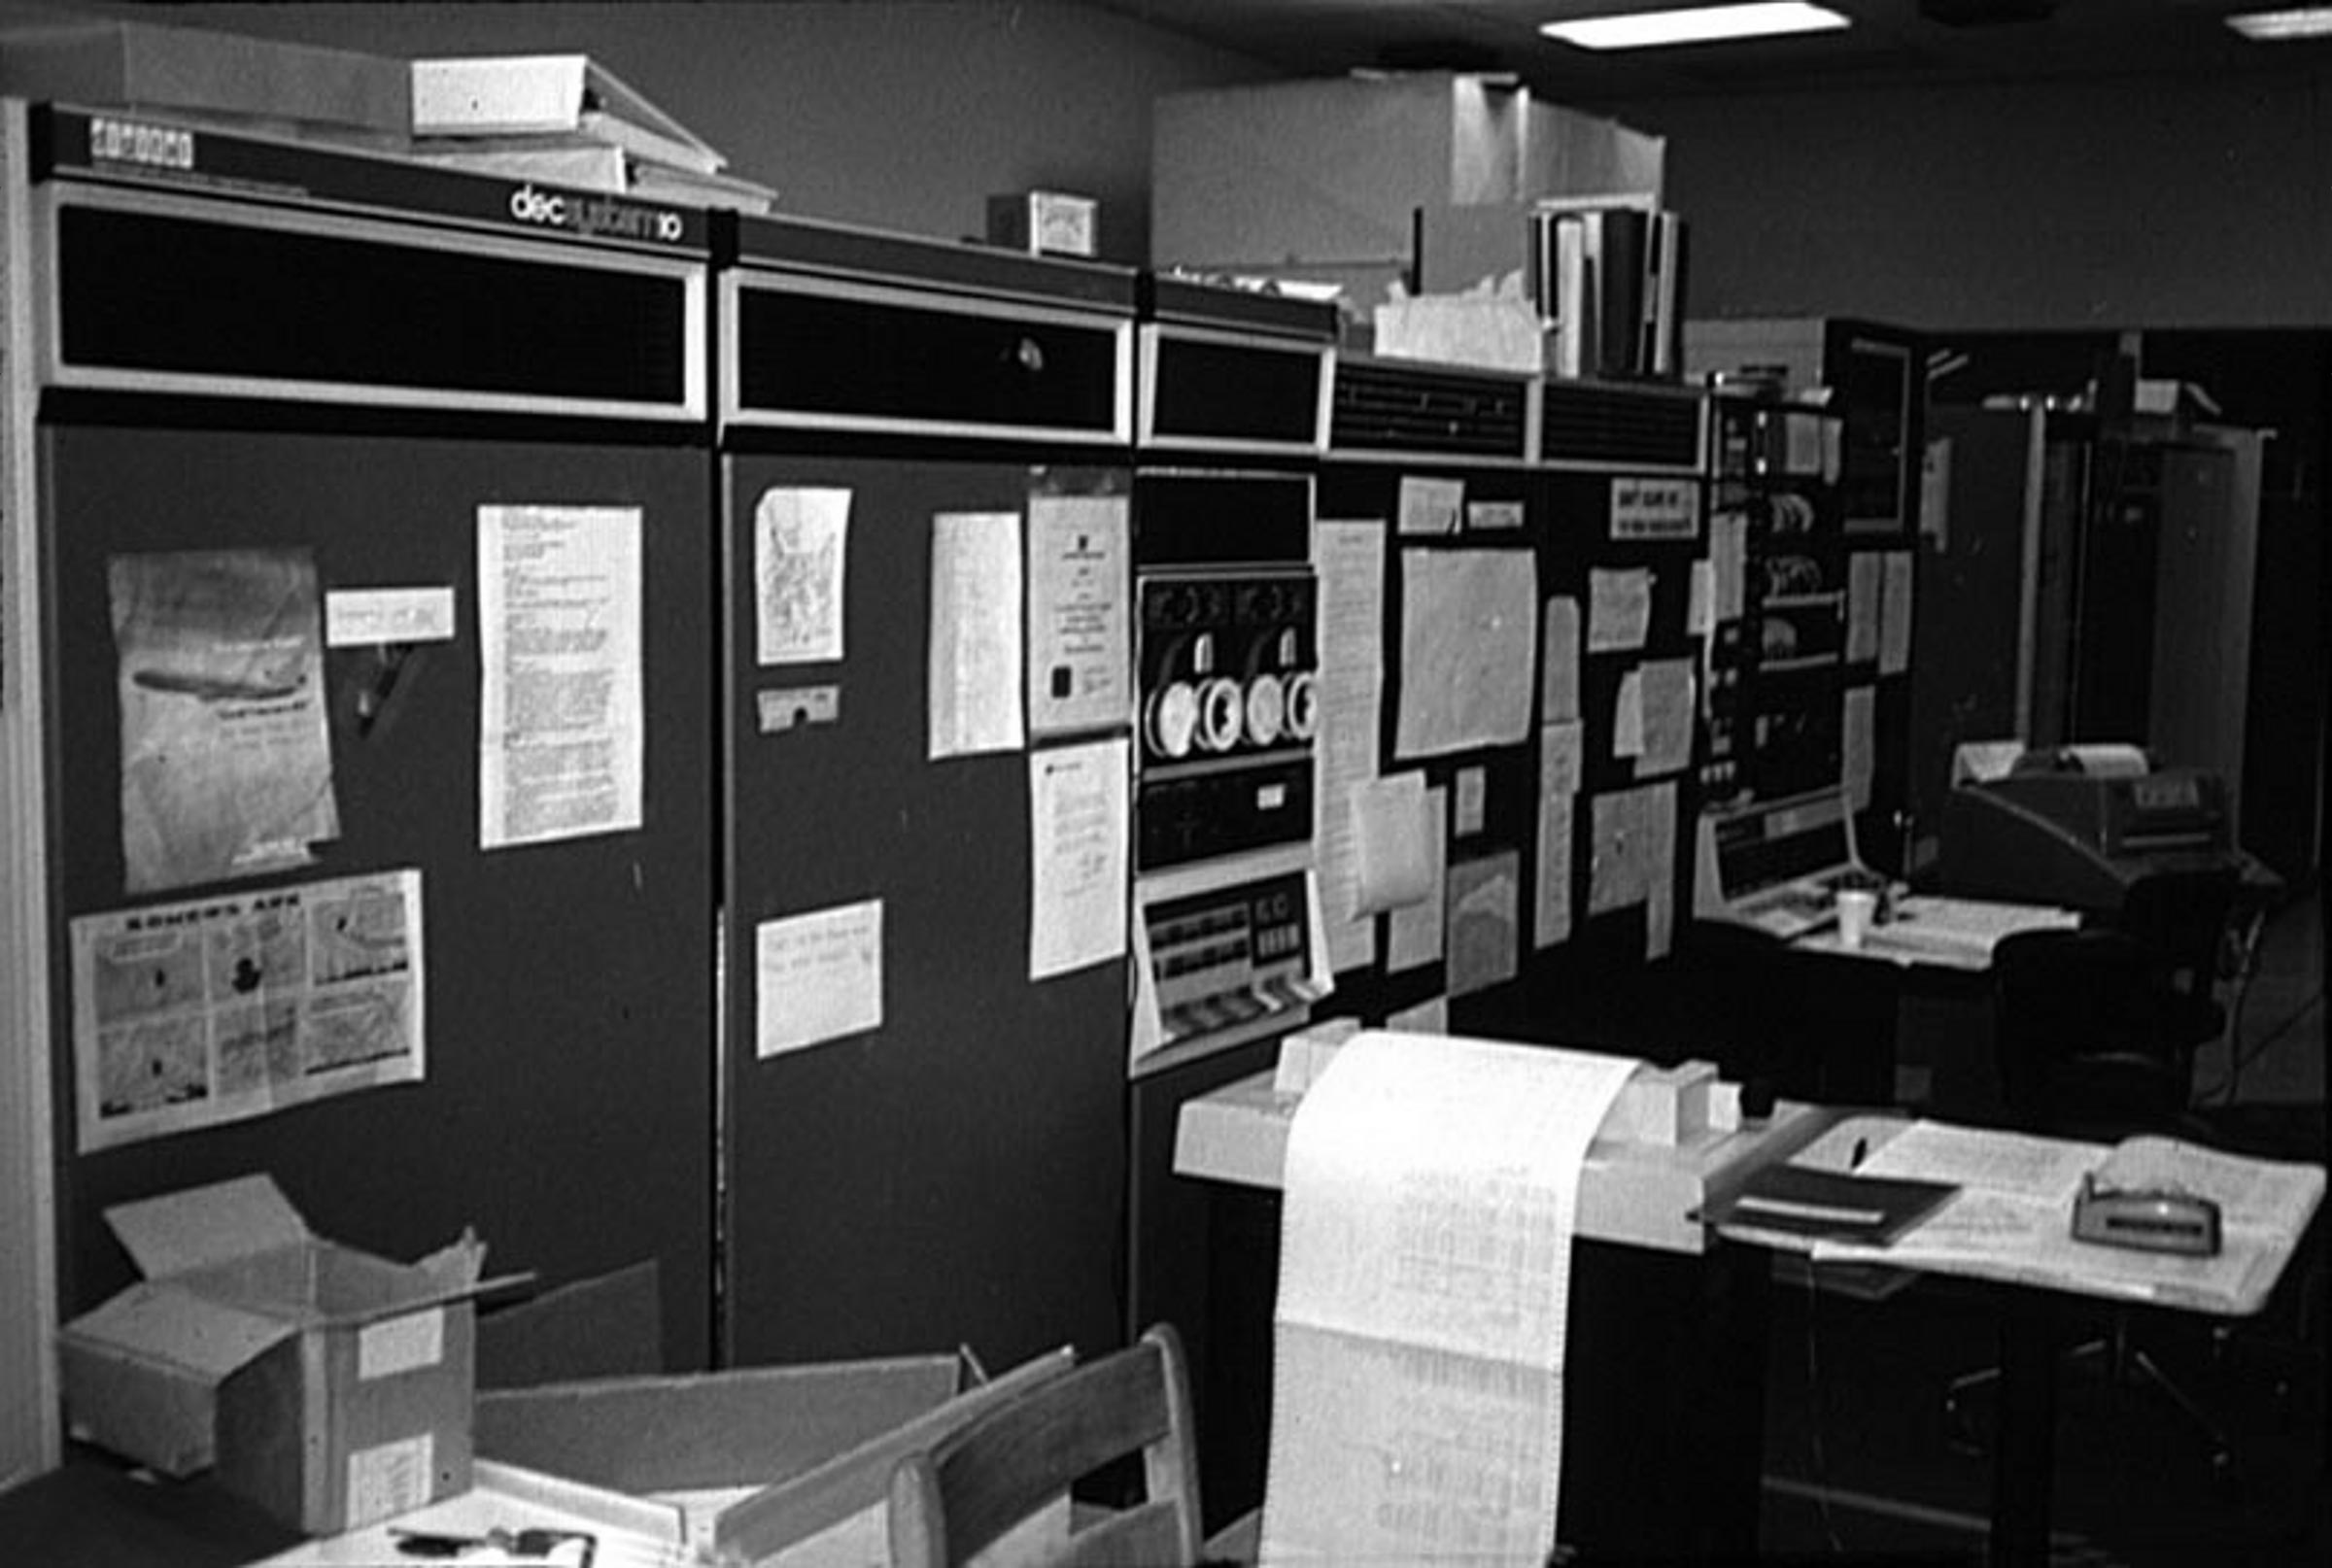
\includegraphics[width=0.8\textwidth]{KL10_1979}
  \caption{\small PDP-10-Rechenanlage mit Zentraleinheit KL-10 (ähnlich der im AI Lab), Stanford Artificial Intelligence Laboratory, 1979.}
\end{figure}

"`Ohne Hacker, die das System warten, haben die [Dozenten] gesagt, \glq Das gibt ein Desaster; wir brauchen kommerzielle Software.\grq\,"', erinnert sich Stallman einige Jahre später. "`Sie haben gesagt \glq Wir können von der Firma erwarten, dass sie es warten.\grq{} Das hat sich als völlig falsch erwiesen, aber sie haben es so gesagt.\comment{but that's what they did}"'\footcite{rmskth}

Zuerst haben die Hacker das Twenenx-System\index{Twenex|(} nur als weiteres Symbol des Autoritarismus angesehen, das danach schreit, umgestürzt zu werden. Der Systemname selbst war schon ein Protest. Das von DEC offiziell so genannte, und nach seinem Vorgänger TOPS-10 benannte, proprietäre Betriebssystem TOPS-20 wurde für die PDP-10 vertrieben. Aber TOPS-20 basierte nicht auf TOPS-10. Es war vom Tenex-System\index{Tenex} abgeleitet, das Bolt Beranek Newman für die PDP-10 entwickelt hatte.\footnote{Mehrere Quellen: Interview mit Richard Stallman, E-Mail von Gerald Sussman und \cite[][Glossary: "`TWENEX"']{jargonf}.} Stallman, der den Begriff "`Twenex"' geprägt hat, sagt, er ist darauf gekommen, weil er den Namen TOPS-20 vermeiden wollte. "`Das System war weit davon entfernt, top zu sein, und deshalb wollte ich es um keinen Preis so nennen"', erinnert sich Stallman. "`Also habe ich mich entschieden, ein \glq w\grq{} in den Namen Tenex einzufügen und es Twenex zu nennen."'

%Zitate aus zwei verschiedenen Szenen aus dem Film von 1939
%Buch: "Ich bin der große und schreckliche Oz."
%"Beachtet nicht weiter den Mann hinter dem Vorhang." -> nicht im Buch
Der Rechner, auf dem das Betriebssystem Twenex/TOPS-20 lief, hatte seinen eigenen spöttischen Spitznamen: Oz. Der Hackerlegende zufolge erhielt der Rechner seinen Namen, weil er eine kleinere PDP-11 benötigte, um das Terminal zu betreiben. Ein Hacker, der den KL-10/PDP-11-Aufbau zum ersten Mal sah, verglich ihn mit der bombastischen filmischen Vorstellung des Zauberers von Oz. "`Ich bin Oz, der große und mächtige"', tönte der Hacker. "`Beachtet nicht weiter die PDP-11 hinter der Konsole."'\footcite[Vgl.][]{fig1}

Auch wenn die Hacker zuerst gelacht haben, wenn sie die KL-10 das erste Mal gesehen haben, sollte ihr Gelächter schnell verstummen, wenn sie es mit Twenex zu tun bekamen. Nicht nur rühmte sich Twenex\index{Twenex|)} seiner integrierten Sicherheitsvorkehrungen, die Systemingenieure hatten die Werkzeuge und Anwendungen auch mit Sicherheitsaspekten im Hinterkopf entworfen. Was einst ein Katz-und-Maus-Spiel wegen Passwörtern auf dem Sicherheitssystem des Laboratory for Computer Science war, war zu einem absoluten Kampf um die Systemverwaltung geworden. Die Systemadministratoren argumentierten, dass das Oz-System ohne Sicherheitsvorkehrungen anfälliger für versehentliche Abstürze wäre. Die Hacker argumentierten, dass das besser durch Überarbeitung des Quellcodes vermieden werden könne. Unglücklicherweise war die Anzahl der Hacker mit der Zeit für und der Neigung zu dieser Art Überarbeitung soweit geschwunden, dass sich die Ansichten der Administratoren durchsetzten.

Anfangs war es Praxis, dass jedes Mitglied des AI Labs das "`Wheel"'-Privileg\index{Wheel}\footnote{Der Begriff taucht das erste mal in TENEX auf und ist die Kurzform für "`big wheel"'. \cite[Vgl.][Glossary: "`wheel"']{jargonf}.} hatte, um die Sicherheitsbeschränkungen zu umgehen. Aber jeder, der das "`Wheel"'-Privileg hatte, konnte es jedem anderen streichen, und dann hatte derjenige keine Möglichkeit mehr, es wiederherzustellen. Diese Situation führte dazu, dass eine kleine Gruppe Hacker versucht war, mit dem Entfernen der "`Wheel"'-Privilegien der anderen die völlige Kontrolle an sich zu reißen.

Durch das Schnorren von Passwörtern und Debuggen konnte Stallman die Vorhaben vereiteln. Nach dem zweiten gescheitertem \textit{Coup d'État} gab Stallman eine Warnung an das AI-Lab-Personal heraus.\footcite[Vgl.][]{rmskth}

"`Es hat wieder einen Versuch gegeben, die Macht zu ergreifen"', schrieb Stallman. "`Fürs Erste sind die aristokratischen Truppen geschlagen."' Um seine Identität zu verschleiern, unterschrieb Stallman die Nachricht mit "`Radio Free OZ"'.

Die Tarnung war bestenfalls dürftig. 1982 war Stallmans Abneigung gegen Passwörter und Geheimhaltung so bekannt geworden, dass Leute außerhalb des AI Laboratory sein Benutzerkonto von überall aus dem ARPAnet nutzten – dem mit Forschungsgeldern finanzierten Computernetzwerk, das dem Internet als Grundlage dienen sollte. Einer dieser "`Touristen"' während dem Anfang der 80er war Don Hopkins\index{Hopkins, Don|(}, ein kalifornischer Programmierer, der über Gerüchte erfahren hatte, dass man sich als Außenstehender einfach mit dem Benutzernamen RMS und demselben Passwort an MITs gepriesenem ITS-System anmelden konnte.

"`Ich bin dem MIT auf ewig dankbar, dass sie mich und viele andere ihre Computer umsonst haben nutzen lassen"', sagt Hopkins\index{Hopkins, Don|)}. "`Es hat einer Menge Leute viel bedeutet"'.

Der sogenannte "`Tourismus"', der von der MIT-Leitung in den ITS-Jahren toleriert wurde,\footcite{mittour} blieb auf der Strecke, als Oz die Hauptverbindung des AI Labs ins ARPAnet wurde. Zuerst hielt Stallman an der Tradition fest, seinen Benutzernamen als Passwort zu verwenden, damit Nutzer von außerhalb Zugang über sein Konto erlangen konnten. Mit der Zeit veranlasste die Instabilität von Oz die Administratoren jedoch dazu, Außenstehende zu blockieren, die versehentlich oder mit Absicht das System abschießen könnten. Als diese Administratoren schließlich von Stallman verlangten, sein Passwort nicht mehr zu veröffentlichen, berief sich Stallman auf seine persönliche Ethik und hörte ganz auf, das System zu benutzen.\footcite[Vgl.][]{rmskth}

"`Seitdem Passwörter im MIT AI~Lab aufgetaucht sind, habe ich [mich entschieden], meiner Überzeugung zu folgen, dass es keine Passwörter geben sollte"', sagt Stallman später. "`Weil ich nicht glaube, dass es wirklich erstrebenswert ist, Sicherheitsmaßnahmen auf einem Computer zu haben, sollte ich nicht gewillt sein, das Aufrechterhalten eines Sicherheitsregimes zu unterstützten."'\footcite{rmskth}

Stallmans Weigerung, sich dem großen und mächtigen Oz zu beugen, symbolisierte die wachsende Spannung zwischen den Hackern und der AI-Lab-Leitung Anfang der 80er. Die Spannung war kein Vergleich zu den Konflikten, die sich in der Hackergemeinschaft selbst abspielten. Als das Decsystem 20 ankam, war die Gemeinschaft in zwei Lager gespalten – LMI und Symbolics.

Symbolics mit seinem Fremdkapital heuerte verschiedene AI-Lab-Hacker an. Einige von ihnen setzte man außerhalb des AI~Labs zur Verbesserung von Betriebssystemteilen der Lisp-Maschine ein. Ende 1980 arbeiteten 14 Mitglieder des AI~Labs in Teilzeit als Berater an der Entwicklung einer eigenen Version der Lisp-Maschine für die Firma. Die wenigen übrigen, außer Stallman, arbeiteten für LMI.\footcite[Vgl.][S.\,423]{hackers} Stallman, der das ungezwungene Leben am AI~Lab bevorzugte und keine Partei ergreifen wollte, entschied sich, keinem der beiden Unternehmen beizutreten.

Zuerst verbrachten die anderen Hacker weiterhin Zeit am MIT und leisteten ihre Beiträge zum Betriebssystem der MIT-Lisp-Maschine. LMI und Symbolics hatten beide den Code vom MIT lizenziert. Die Lizenz erforderte es, dass sie ihre Änderungen an das MIT zurückgeben, aber sie mussten es dem MIT nicht erlauben, diese Änderungen weiterzuverbreiten. Jedoch hielten sie sich bis 1981 an ein Gentlemen's Agreement, dass es zuließ, und so konnten alle Systemverbesserungen in die MIT-Version eingehen und mit allen Nutzern von Lisp-Maschinen geteilt werden. Diese Situation erlaubte es den am MIT Verbliebenen, neutral zu bleiben.

Am 16. März 1982, erinnert sich Stallman, weil es an seinem Geburtstag war, kündigte Symbolics das Gentlemen's Agreement auf. Das Motiv war ein Angriff auf LMI. LMI hatte weniger Hacker und allgemein weniger Personal, also dachte der Symbolics-Vorstand, dass LMI den größten Vorteil aus dem Teilen der Verbesserungen zog. Mit der Aufkündigung des Systemcodeaustausches hofften sie, LMI auszulöschen. Sie entschieden sich, die Lizenz exakt durchzusetzen. Statt ihre Verbesserungen in die MIT-Version des Systems einzuarbeiten, welches LMI nutzen konnte, stellten sie dem MIT eine Kopie der Symbolics-Version des Systems zur Verfügung\comment{, die die Nutzer am MIT verwenden konnten}. Jeder, der das System benutzte, würde nur für Symbolics Testarbeit leisten, und wenn er Verbesserungen machte, wären sie höchstwahrscheinlich auch nur für Symbolics von Nutzen.

Als Verantwortlicher (in den ersten Monaten mit Hilfe Greenblatts\index{Greenblatt, Richard}) für die Wartung der Lisp-Maschinen im Labor war Stallman empört. Die Symbolics-Hacker hatten den Code des Systems mit hunderten halbfertigen Änderungen zurückgelassen, die Fehler verursachten. Er sah diese Ankündigung als "`Ultimatum"' an und revanchierte sich, indem er Symbolics' Richtfunkverbindung\comment{microwave communications link} zum AI~Lab kappte. Er schwor sich, nie wieder an einer Symbolics-Maschine zu arbeiten und das MIT-System weiterzuentwickeln, um LMI gegen Symbolics zu verteidigen. "`So wie ich es gesehen habe, war das AI~Lab neutrales Territorium wie Belgien im Zweiten Weltkrieg"', sagt Stallman. "`Wenn Deutschland in Belgien einfällt, dann erklärt Belgien Deutschland den Krieg und verbündet sich mit Britannien und Frankreich."'

Als der Symbolics-Vorstand merkte, dass ihre neuesten Funktionen immer noch auf den Lisp-Maschinen des MIT auftauchten und somit auch in den Lisp-Maschinen von LMI, waren sie nicht erfreut. Stallman wusste, was das Urheberrecht erfordert, und schrieb die Funktionen komplett neu. Er nutzte die Möglichkeit aus, sich den Quellcode anzuschauen, den Symbolics dem MIT zur Verfügung stellte, so dass er die Probleme und ihre Lösungen verstand, und achtete dann darauf, seine Änderungen auf eine ganz andere Weise zu schreiben. Der Symbolics-Vorstand wollte das nicht glauben. Sie installierten ein "`Spionage"'-Programm auf Stallmans Terminal, das nach Beweisen gegen ihn suchen sollte. Als sie ihr Anliegen dann der MIT-Leitung vorbrachten, etwa Anfang 1983, hatten sie wenig Beweise vorzuweisen: ein Dutzend Stellen im Quellcode, an denen beide Versionen geändert wurden und ähnlich aussahen.

Als die Leiter des AI~Labs Stallman die mutmaßlichen Beweise von Symbolics zeigten, entkräftete er sie, indem er bewies, dass die Ähnlichkeiten in Wirklichkeit Relikte aus der Zeit vor dem Fork waren. Und er drehte ihre Logik um: wenn Symbolics bei den tausenden Zeilen, die er geschrieben hatte, mit keinen besseren Beweisen aufwarten konnte, wies das nach, dass seine sorgfältigen Anstrengungen, Plagiate zu vermeiden, wirksam waren. Das AI~Lab hieß Stallmans Arbeit gut, und er führte sie bis Ende 1983 fort.\footnote{Im Buch \citefield{title}{brainm} behauptet der Autor \citeauthor{brainm} fälschlich, dass das AI~Lab ihn angewiesen hat, sich aus dem Lisp-Maschinen-Projekt herauszuhalten.}

Dennoch änderte Stallman seine Taktik. "`Nur um ultrasicher zu sein, habe ich deren Quellcode nicht mehr gelesen. Ich habe nur die Dokumentation [als Grundlage] verwendet und den Code damit geschrieben."'  Die größten neuen Funktionen entwarf er selbst, ohne auf die Veröffentlichung der Dokumentation von Symbolics zu warten. Wenn die Dokumentation dann erschien, machte er sie mit der Symbolics-Schnittstelle für die Funktion kompatibel. Danach las er Symbolics' Quellcodeänderungen, um auch kleinere Fehler zu finden, die sie behoben hatten, und behob sie selbst auf eine andere Art.

Die Erfahrung stärkte Stallmans Entschlossenheit. Stallman heuerte außerdem Mitglieder des AI~Labs an, die das MIT-System weiter nutzen sollten, damit der Fluss an Fehlerreports für seine Ersatzfunktionen nicht abbricht. Das MIT gewährte LMI weiterhin direkten Zugriff auf die Änderungen. "`Ich wollte Symbolics bestrafen, auch wenn es das letzte sein sollte, was ich tue"', sagt Stallman. Solche Äußerungen sind aufschlussreich. Sie bringen nicht nur Licht an Stallmans nichtpazifistische Natur, sie spiegeln auch die intensiven Gefühle wider, die der Konflikt bei ihm ausgelöst hat.

Das Ausmaß der Verzweiflung war stark dem geschuldet, was Stallman als "`Zerstörung"' seines "`Zuhauses"' betrachtete – dem Niedergang der eng verbundenen Hackersubkultur. In einer der letzten Interview-E-Mails sollte sich Stallman mit der historischen Figur Ishi vergleichen, dem letzten überlebenden Mitglied der Yahi, einem Indianerstamm im Pazifischen Nordwesten, der in den Indianerkriegen in den 1860ern und 1870ern ausgerottet wurde. Die Analogie stellt Stallmans Überleben in ein episches, fast mythisches Licht.\footnote{Steven Levy hatte in \citefield{shorttitle}{hackers} diese Zeit im Sinn, als er Stallman als den "`letzten echten Hacker"' bezeichnete, aber die beabsichtigte Bedeutung ist anders, als man vielleicht denken mag. Levy benutzte den Begriff "`echte Hacker"' zur Unterscheidung der MIT-Hackergemeinde von den zwei anderen Hackergemeinden im Buch, die später beschrieben werden und die er anders bezeichnet. Als sich seine Gemeinde aufgelöst hatte und nur Stallman übrig war, wurde er damit zum letzten "`echten Hacker"'. Levy meint nicht, dass niemand sonst ein wahrhaftiger Hacker ist, aber man scheint es meist so zu interpretieren\comment{, besonders die Leute, die sich nicht die Erläuterungen in Levys Buch durchlesen}. Stallman selbst hat sich nie mit diesen Worten beschrieben.} Die Hacker, die für Symbolics arbeiteten, sahen das anders. Statt Symbolics als zerstörerische Kraft anzusehen, sahen es viele Kollegen Stallmans als späten Versuch, sich Geltung zu verschaffen. Mit der Kommerzialisierung der Lisp-Maschine hatte die Firma die Hackerprinzipien des ingenieurgetriebenen Softwaredesigns aus dem Elfenbeinturm des AI~Labs in den Unternehmensmarkt gedrängt, auf dem die Designprinzipien der Manager vorherrschten. Statt Stallman als einen Verweigerer zu sehen, sahen viele in ihm einen Repräsentanten einer veralteten Praxis.

Auch persönliche Feindseligkeiten spielten eine Rolle. Selbst bevor Symbolics die meisten AI-Lab-Hacker abgeworben hatte, sagt Stallman, hätten ihn viele der Hacker, die später zu Symbolics gehen sollten, gemieden. "`Man hat mich nicht mehr nach Chinatown eingeladen"', entsinnt sich Stallman. "`Der von Greenblatt gestartete Brauch war, dass wenn man auswärts zu Abend isst, man herumgeht und die anderen im Lab fragt oder eine Nachricht schickt, ob sie auch mitkommen wollen. Irgendwann um 1980-1981 hat es aufgehört, dass ich gefragt wurde. Sie haben mich nicht nur nicht gefragt, aber jemand hat mir später gestanden, dass er unter Druck gesetzt worden ist, mich zu belügen und das Essengehen ohne mich geheimzuhalten."'

Obwohl sich Stallman von dieser engstirnigen Form der Ausschließung verletzt fühlte, konnte er nichts dagegen tun. Das Ultimatum von Symbolics änderte den Sachverhalt von einer persönlichen Ablehnung zu einer größeren Ungerechtigkeit. Als Symbolics seine Quellcodeänderungen von der Weiterverbreitung ausnahm, um seinen Rivalen zu schlagen, entschied sich Stallman, ihre Pläne zu durchkreuzen. Indem er mit seinen Aufgaben am MIT durchhält und ein Gegenstück zu jeder neuen Softwarefunktion und jedem Fix schreibt, wollte er den Nutzern des MIT-Systems, einschließlich den LMI-Kunden, dieselbe Funktionalität geben, die die Symbolics-Nutzer hatten.

Außerdem würde es Stallmans Status als Legende in der Hackergemeinde sichern sollen. Schon damals war er berühmt für seine Arbeit an Emacs, und seine Fähigkeit, mit der Arbeitsleistung eines ganzen Teams von Symbolics-Programmierern gleichzuziehen – einem Team, das selbst mehr als nur ein paar legendäre Hacker umfasste – steht heute immer noch als eine der größten Leistungen des Informationszeitalters, oder jedes Zeitalters. Steven Levy bezeichnete es als einen "`Meister-Hack"' und Stallman selbst als einen "`virtuellen John Henry des Computercodes"'.\footnote{John Henry ist ein US-amerikanischer Folkloreheld, der in einem Wettkampf bei Gleisverlegearbeiten gegen einen Dampfhammer gewonnen haben soll.} Er merkt an, dass selbst seine bei Symbolics angestellten Rivalen keine Wahl hatten, als ihrem idealistischen alten Kameraden widerwillig Respekt zu zollen. Levy zitiert Bill Gosper\index{Gosper, Ralph William \glq Bill\grq}, einen Hacker, der in ihrem Büro in Palo Alto für Symbolics arbeitete, wie er sein Erstaunen über Stallmans Programmierleistungen in dieser Phase ausdrückt:

\begin{quote}
Ich sah etwas, was Stallman geschrieben hat, und ich würde es vielleicht für schlecht befinden (eher nicht, aber man könnte mich überzeugen, dass es schlecht war), aber dann würde ich immer noch sagen, "`Ja, Moment mal – Stallman hat da drüben niemanden, mit dem er die ganze Nacht diskutieren kann. Er arbeitet allein! Es ist unglaublich, dass jemand das alles allein machen kann!"'\footcite[Vgl.][S.\,426]{hackers}
\end{quote}

%machine room - 
Für Stallman rufen die Monate, die er damit verbracht hat, mit Symbolics aufzuholen, eine Mischung aus Stolz und tiefer Traurigkeit hervor. Stallman, ausgemachter Linker, dessen Vater im Zweiten Weltkrieg gedient hatte, ist kein Pazifist. In vielerlei Hinsicht war der Symbolics-Krieg der Initiationsritus, auf den Stallman seit Beginn seiner Anstellung am AI~Lab ein Jahrzehnt zuvor hingeschlittert ist. Und gleichzeitig fiel er mit der traumatischen Zerstörung der Hackerkultur am AI~Lab zusammen, die Stallman seit seiner Jugend aufgezogen hatte. Eines Tages, als er eine Programmierpause machte, hatte Stallman ein traumatisches Erlebnis beim Durchgehen durch den Rechnerraum des Labs. Dort sah Stallman das klobige, ungenutzte Gehäuse einer PDP-10. Bestürzt über die erloschenen Lämpchen, die einst eifrig blinkten und den internen Zustand von Systemprogrammen anzeigten, war der emotionale Einfluss auf Stallman ähnlich dem, ein geliebtes Familienmitglied aufgebahrt zu sehen.

"`Ich habe direkt dort im Rechnerraum angefangen, zu weinen"', sagt er. "`Die Maschine dort zu sehen, tot, ohne jemanden, der sie reparieren kann, hat mir klargemacht, wie völlig zerstört meine Gemeinde gewesen ist."'

Stallman sollte wenig Zeit zum Trauern bleiben. Die Lisp-Maschine war, trotz all dem Aufruhr um sie und all der Arbeit, die in ihre Entwicklung geflossen ist, nur ein Nebenkriegsschauplatz in der größeren Schlacht auf dem technologischen Markt. Die unermüdliche Geschwindigkeit der Computerminiaturisierung brachte immer neue, leistungsfähigere Mikroprozessoren hervor\comment{, die die Hardware- und Softwarefähigkeiten der Maschine verschlingen würde wie eine moderne Metropole ein vorzeitliches Wüstendorf XXX would soon incorporate the machine's hardware and software capabilities like a modern metropolis swallowing up an ancient desert village}.

Mit dieser Welle kamen hunderte, ja tausende, proprietäre Softwareprogramme, jedes davon geschützt durch ein Geflecht an Endnutzer-Lizenzvereinbarungen und Geheimhaltungsverträgen, das es Hackern unmöglich machte, den Quellcode zu begutachten oder auszutauschen. Die Lizenzen waren krude und unpassend, aber bis 1983 waren sie gut genug geworden, dass sie in Gerichten anerkannt wurden und Eindringlinge fernhielten. Software, einst eine kostenlose Beilage von den meisten Hardwarefirmen, um ihre teuren Computersysteme den Kunden schmackhafter zu machen, wurde schnell zum Hauptgericht. Bei ihrem wachsenden Heißhunger nach neuen Spielen und Funktionen brachen die Nutzer mit der Tradition, nach jeder Mahlzeit nach dem Rezept zu verlangen.

Nirgendwo war dieser Umstand offenkundiger als im Reich der PC-Systeme. Firmen wie Apple Computer und Commodore brachten mit dem Verkauf von Rechnern mit vorinstalliertem Betriebssystem frischgebackene Millionäre hervor. Viele Nutzer waren nicht vertraut mit der Hackerkultur und ihrer Abneigung gegenüber rein in Maschinencode verbreiteter Software und viele sahen keinen Anlass, sich bei den Firmen wegen des Fehlens von beigelegtem Quellcode zu beschweren. Einige anarchische Anhänger der Hackerethik versuchten sie in diesen neuen Markt einzuführen, aber der Markt belohnte größtenteils nur die Programmierer, die schnell genug waren, neue Programme zu schreiben und gerissen genug, Endnutzerlizenzverträge zu schreiben, um sie gut abzusichern.

Einer der bekanntesten dieser Programmierer war Bill Gates, ein Harvard-Abbrecher und zwei Jahre jünger als Stallman. Obwohl Stallman ihn zu der Zeit nicht kannte, sieben Jahre, bevor er seine Nachricht an die Newsgroup thenet.unix-wizards schickte, hatte Gates, ein Jungunternehmer und Komplementär\comment{general partner} der in Albuquerque ansässigen Softwarefirma Micro-Soft, später "`Microsoft"' geschrieben, einen offen Brief an die Softwaregemeinde\comment{software-developer community} geschickt. Er war die Reaktion auf PC-Nutzer, die Micro-Softs Programme kopieren, und Gates greift in seinem \citefield{shorttitle}{gatesletter} die Vorstellung gemeinschaftlicher Softwareentwicklung heftig an.

"`Wer kann es sich leisten, professionelle Arbeit umsonst zu leisten?"', fragt Gates. "`Welcher [Hobbyprogrammierer] kann drei Arbeitsjahre in die Programmierung stecken, in das Auffinden aller Fehler, das Dokumentieren seines Produkts und es umsonst verbreiten?"'\footcite[Vgl.][]{gatesletter}

Obwohl nur wenige Hacker im AI~Lab das Kommuniqué gelesen hatten, repräsentierte Gates' Brief von 1976 die sich wandelnde Einstellung zu Software, gleichermaßen unter kommerziellen Softwarefirmen als auch Entwicklern kommerzieller Software. Warum sollte man Software als Gratisware ansehen, wenn der Markt eine andere Sprache spricht? Als die 70er den 80ern wichen, wurde der Verkauf von Software mehr als nur ein Weg, seine Kosten zu decken; er wurde zu einer politischen Aussage. Es war die Zeit, als sich das Kabinett Reagon daran gemacht hatte, viele der föderalen Vorschriften und staatlichen Förderprogramme zu demontierten, die in dem halben Jahrhundert nach der Weltwirtschaftskrise aufgebaut worden waren. Mehr als nur ein paar Programmierer sahen die Hackerethik als wettbewerbsfeindlich an und daher als unamerikanisch. Bestenfalls war sie eine Rückkehr zu den antiindustriellen Haltungen der späten 60er und frühen 70er. Wie ein Wall-Street-Banker, der ein altes Batikshirt zwischen seinen Manschettenhemden und Zweireihern findet, sahen die meisten Programmierer die Hackerethik als peinliches Erinnerungsstück an das idealistische Zeitalter\comment{Alter?}.

%????? throwback to the 50s
%stark moral - rein moralisch?
\comment{For a man who had spent the entire 1960s as a throwback to the 1950s,}Stallman störte es nicht, aus der Reihe zu tanzen. Als Programmierer, der es gewöhnt war, an den besten Rechnern mit der besten Software zu arbeiten, stand Stallman jedoch vor einer "`schwerwiegenden moralischen Entscheidung"': entweder seine ethischen Einwände gegen "`proprietäre"' Software hinunterzuschlucken – den Begriff nutzten er und seine Hackerkollegen als Bezeichnung aller Programme, die einen Copyrightvermerk oder eine andere Lizenz tragen, welche das Kopieren und Ändern einschränkt  – oder sein Leben der Schaffung eines alternativen, nicht proprietären Systems zu widmen. Nach seinem zweijährigen Krieg gegen Symbolics fühlte  Stallman sich zuversichtlich genug, letztere Option zu wählen. "`Ich halte es für möglich, dass ich ganz hätte aufhören können, im Computerbereich zu arbeiten"', sagt Stallman. "`Ich hatte keine besonderen Fähigkeiten, aber ich hätte sicherlich Kellner werden können. In einem feinen Restaurant wahrscheinlich nicht, aber irgendwo hätte ich Kellner sein können."'

Zu kellnern und das Programmieren ganz aufzugeben, wäre der Verlust einer Tätigkeit gewesen, die ihm so viel Freude bereitet hatte. Wenn Stallman zurückblickt auf sein Leben nach dem Umzug nach Cambridge, kann er leicht lange Phasen ausmachen, in denen das Programmieren seine einzige Freude gewesen ist. Statt auszusteigen, entscheidet sich Stallman, dranzubleiben.

Als Atheist lehnt Stallman Vorstellungen wie Schicksal, Karma und göttliche Berufung ab. Dennoch hält er die Entscheidung für naturgemäß, sich von proprietärer Software fernzuhalten und ein Betriebssystem zu schaffen, das auch anderen dabei hilft. Im Endeffekt war es Stallmans persönliche Kombination aus Dickköpfigkeit, Weitblick und programmiererischem Können, die ihn einen Weg erwägen haben lassen, den die meisten anderen nicht gesehen haben. In seinem Artikel \citefield{title}{rmsgnupr} drückt Stallman Übereinstimmung mit den Idealen aus, die in den Zeilen des Jüdischen Weisen Hillel stecken:

\begin{quote}
Wenn ich nicht für mich bin, wer ist für mich? und wenn ich für mich bin, was bin ich? und wenn nicht jetzt, wann denn?\footcite[Vgl.][S.\,108 Mischna XII.-XIV]{thalmud}\,\footnote{\cite[Vgl.][]{rmsgnupr}. Stallman fügt seine eigene Fußnote hinzu: "`Als Atheist folge ich keinen religiösen Führern, aber manchmal bewundere ich etwas, was sie gesagt haben."'}
\end{quote}

Beim Reden zum Publikum vermeidet Stallman den religiösen Weg und legt seine Entscheidung pragmatisch aus. "`Ich habe mich gefragt: was kann ich als Betriebssystementwickler tun, um die Lage zu verbessern? Erst als ich die Frage eine Weile untersucht hatte, habe ich gemerkt, dass ein Betriebssystementwickler genau das war, was man zur Lösung des Problems braucht."'

Als er das erkannt hatte, wurde Stallman alles andere ganz klar. 1983 kaufte das  MIT eine Lisp-Maschine der 2.\,Generation von Symbolics, auf der das MIT-Lisp-System nicht laufen konnte. Als die meisten MIT-Rechner ersetzt worden waren, konnte er das System nicht mehr effektiv warten, weil ihm die Fehlerreports der Nutzer fehlten. Er musste aufhören. Aber er wollte auch aufhören. Das System der MIT-Lisp-Maschine war keine freie Software: selbst obwohl die Nutzer den Quellcode bekommen konnten, durften sie ihn nicht frei weiterverbreiten. Inzwischen war das Ziel hinter der Weiterführung des MIT-Systems erreicht: LMI hatte überlebt und entwickelte selbst Software.

Stallman wollte nicht den Rest seines Lebens damit verbringen, diejenigen zu bestrafen, die seine alte Gemeinde zerstört hatten. Er wollte eine neue aufbauen. Er entschied sich, Software anzuprangern, die seine ethischen Vorstellungen verletzt, und sein Leben der Schaffung von Programmen zu widmen, die es ihm und anderen erleichtern, von ihr fernzubleiben. Mit dem Schwur, ein freies Betriebssystem zu entwickeln "`und wenn ich dabei sterbe – am hohen Alter, natürlich"', witzelt Stallman, kündigte er im Januar 1984 beim MIT, um GNU zu entwickeln.

Die Kündigung entzog Stallman der rechtlichen Schirmherrschaft des MIT. Trotzdem hatte Stallman immer noch genug Freunde und Verbündete am AI~Lab, dass er weiterhin die Einrichtung nutzen konnte und später ein eigenes Büro. Er hatte außerdem die Möglichkeit, sich externe Berateraufträge zu beschaffen, um das GNU Project in seiner Frühphase zu finanzieren. Mit der Kündigung am MIT hatte Stallman jedoch jede Debatte um den Interessenkonflikt und das Fallen der Verbreitungsrechte der Software ans MIT verhindert. Der Mann, dessen Furcht vor sozialer Isolation ihn immer weiter in die Arme des AI~Labs getrieben hatte, baute nun eine rechtliche Brandschutzmauer zwischen sich und diese Umgebung.

In den ersten Monaten arbeitete Stallman auch in Isolation von der Unix-Gemeinde. Obwohl seine Ankündigung auf der Newsgroup net.unix-wizards wohlwollende Reaktionen hervorgerufen hatte, hatten sich nur wenige Freiwillige gefunden, die sich in der Anfangsphase mit ihm auf den Kreuzzug machen wollten.

"`Die Reaktion der Gemeinde war ziemlich unisono"', erinnert sich Rich Morin\index{Morin, Richard \glq Rich\grq}, damals Leiter einer Unix User Group. "`Die Leute meinten, \glq Oh, das ist eine hervorragende Idee. Zeig uns deinen Code. Zeig uns, dass es möglich ist.\grq\,"'

Im Bewusstsein, dass seine Aufgabe enorm war, entschied sich Stallman, soviel bestehende freie Software wie möglich wiederzuverwenden. Und so begann er, nach \comment{existing free} Programmen und Werkzeugen zu suchen, um sie in GNU-Programme und -Werkzeuge umzuwandeln. Einer der ersten Kandidaten war ein C-Compiler namens VUCK\index{VUCK|(}\comment{,which converted programs written in the popular C programming language into machine-runnable code}. Der Name war dänisch für Free University Compiler Kit. Frohen Mutes fragte Stallman den Programmautor,\footnote{Andrew Tanenbaum, vgl. Seite \pageref{Tanenbaum}.}\index{Tanenbaum, Andrew} ob das Programm frei sei. Die Mitteilung des Autors, dass sich die Worte "`Free University"' auf die Vrije Universiteit in Amsterdam beziehen und dass das Programm nicht frei war, machte Stallman verdrossen.

%\url{http://oreilly.com/catalog/opensources/book/stallman.html}
"`Er hat spöttisch geantwortet, dass die Universität frei wäre, aber nicht der Compiler"', erinnert sich Stallman. Er hatte sich nicht nur geweigert zu helfen – er schlug Stallman auch noch vor, seinen Plan eines GNU-Systems aufzugeben und stattdessen Erweiterungen für VUCK zu schreiben, um den Verkauf anzukurbeln; dafür sollte er einen Anteil an den Profiten erhalten. "`Ich habe mich deshalb entschieden, dass mein erstes Programm für das GNU Project ein Compiler für mehrere Sprachen und Plattformen sein wird."'\footcitet[Vgl.][S.\,65: Richard Stallman: \textit{The GNU Operating System and the Free Software Movement}]{opensrc}

% Pastel-Beschreibung geändert lt. http://www.gnu.org/gnu/thegnuproject.html
% XXX Motorola 68010 oder 68000
Als Ersatz für VUCK\index{VUCK|)} fand Stallman den Compiler Pastel\index{Pastel} (ein "`blasses Pascal"'), geschrieben von Programmierern am Lawrence Livermore National Lab. Laut ihnen war der Compiler frei kopier- und modifizierbar, als sie ihm eine Kopie gaben. Leider erwies sich das Programm als ungeeignet, weil seine Speicheranforderungen enorm waren. Es parste die gesamte Eingabedatei in einen Syntaxbaum im Speicher, wandelte ihn in Instruktionen um und schrieb dann die Ausgabedatei; alles, ohne zwischendurch Speicher freizugeben. Auf einem Mainframe-System war das verzeihbar gewesen. Aber auf Unix-Systemen war es eine kaum überwindbare Barriere, weil selbst 32-Bit-Rechner mit Unix oft nicht in der Lage waren, einem Programm so viel Speicher zur Verfügung zu stellen. Stallman machte anfangs schnell erhebliche Fortschritte mit dem Aufbau eines C-Frontends zum Compiler und Tests auf einer größeren Vax, dessen System mit so großen Speicherbereichen zurechtkam. Als er es auf das Motorola-68000-System portieren wollte und den Abstürzen nachging, entdeckte er das Speicherproblem. Er schloss daraus, dass er den Compiler völlig neu schreiben würde müssen. Stallman hat das schließlich in die Tat umgesetzt und den GNU C~Compiler, GCC\index{GCC}, geschaffen. Aber 1984 blieb es ungeklärt, was mit dem Compiler geschehen sollte, und er entschied sich, seine Pläne etwas reifen zu lassen und sich erst anderen Teilen von GNU zu widmen.

Im September 1984 startete Stallman die Entwicklung der GNU-Version von Emacs, den Ersatz für das Programm, das schon ein Jahrzehnt lang unter seiner Ägide lag. In der Unix-Gemeinde waren die zwei nativen Editoren vi von einem Mitbegründer von Sun Microsystems, Bill Joy, und ed vom Bell-Labs-Forscher (und Unix-Urvater) Ken Thompson. Beide waren benutzbar und populär, aber keiner von beiden war so grenzenlos erweiterbar wie Emacs.

Im Nachhinein sagt Stallman, er traf die Entscheidung nicht aus strategischen Gründen. "`Ich wollte ein Emacs, und ich hatte eine gute Gelegenheit, eins zu entwickeln."'

%http://www.gnu.org/gnu/rms-lisp.html
Wieder hatte Stallman eine schon vorhandene Implementierung gefunden, mit dessen Code er sich Zeit zu sparen hoffte.\comment{In writing a Unix version of Emacs,} Stallman folgte in den Fußstapfen eines Postgraduierten an der Carnegie Mellon, James Gosling,\index{Gosling, James|(}\footnote{James Gosling gilt als Erfinder der Programmiersprache Java, arbeitete von 1984 bis zur Aquise 2010 durch Oracle bei Sun Microsystems und seit 2011 bei Google.} Autor einer C-basierten Version namens Gosling Emacs, kurz Gosmacs\index{Gosmacs|(}. Goslings Emacs-Version enthielt einen Interpreter für eine vereinfachten Ableger der Sprache Lisp, Mocklisp. Gosling hatte Gosmacs copyrechtlich geschützt und die Rechte an UniPress verkauft, eine private Softwarefirma. Aber Stallman hatte von einem Kollegen, der anfangs an der Entwicklung von Gosmacs mitarbeitete, eine Zusicherung erhalten. Laut dem Entwickler hatte Gosling, damals als Doktorand, ihm per E-Mail die Erlaubnis erteilt, seine eigene Gosmacs-Version zu verbreiten\comment{in exchange for his contribution to the code}.

Zuerst dachte Stallman, er müsste nur die Benutzerbefehle ändern, um volle Kompatibilität mit dem originalen PDP-1-Emacs zu erreichen. Doch dann merkte er, wie schwach Mocklisp im Vergleich zum echten Lisp war, und war dazu gezwungen, es durch ein echtes Lisp-System zu ersetzen. Dadurch war es naheliegend, den meisten Higher-level-Code von Gosmacs auf eine völlig andere Art neu zu schreiben, um den größeren Funktionsumfang und die flexiblen Datenstrukturen von Lisp auszunutzen. Mitte 1985, als GNU Emacs ins Internet gestellt wurde, hatten nur noch wenige Dateien verbleibenden Code von Gosmacs.

Dann bekam UniPress von Stallmans Projekt Wind und stritt ab, dass der andere Entwickler die Erlaubnis erhalten hatte, seine eigene Version von Gosmacs zu verbreiten. Er konnte die alte E-Mail nicht mehr finden, die seine Behauptung gestützt hätte. Und so entschied sich Stallman, die letzten verbleibenden Module von Gosmacs neu zu schreiben und so das Problem zu beseitigen.

Trotzdem wurmte Stallman die Vorstellung, dass Entwickler die Rechte an ihrer Software verkaufen – dass sie solche Verkaufsrechte überhaupt haben. In einer Rede am Swedish Royal Technical Institute im Jahr 1986 führt Stallman den Vorfall mit UniPress als ein weiteres Beispiel der Gefahren im Zusammenhang mit proprietärer Software an.

"`Manchmal denke ich, es wäre vielleicht das beste, was ich mit meinem Leben anstellen könnte, wenn ich einen gigantischen Haufen proprietärer Software finden würde, die dem Geschäftsgeheimnis unterliegt, und sie dann an der Straßenecke verteilen würde, damit sie kein Geschäftsgeheimnis mehr ist"', sagt Stallman. "`Vielleicht wäre das eine viel effizientere Methode für mich gewesen, den Leuten neue freie Software zu geben, als sie selber zu schreiben; aber alle sind sogar zu feige, sie zu nehmen."'\footcite[Vgl.][]{rmskth}

% reward - Lohn
Trotz des Stresses, den es wegen Goslings\index{Gosling, James|)} Codes gab, sollte der Streit Stallman und der Free-Software-Bewegung langfristig nützen. Er zwang Stallman dazu, die Schwächen der Emacs-Kommune anzugehen und des informellen Vertrauensnetzes, das es ermöglicht hatte, dass problematische Ableger entstehen. Es zwang ihn auch, an den politischen Zielen der Free-Software-Bewegung zu schleifen. Nach der Veröffentlichung von GNU Emacs 1985 gab Stallman das \citefield{title}{gnumani}\index{GNU Manifesto} heraus, eine Erweiterung der ersten Ankündigung vom September 1983. Stallman fügte einen langen Abschnitt mit den vielen Argumenten an, die von kommerziellen und akademischen Programmierern zur Rechtfertigung proprietärer Software genutzt werden. Ein Argument, "`Verdienen Programmierer nicht einen Lohn für ihre Kreativität?"', brachte sich eine Erwiderung ein, die Stallmans Wut über den jüngsten Gosmacs\index{Gosmacs|)}-Vorfall zusammenfasste:

"`Wenn etwas einen Lohn verdient, dann ist es gesellschaftlicher Beitrag"', schreibt Stallman. "`Kreativität kann ein gesellschaftlicher Beitrag sein, aber nur in so fern [\textit{sic}], wie die Gesellschaft frei ist, die Ergebnisse zu nutzen. Wenn Programmierer einen Lohn für das Schaffen innovativer Programme verdienen, dann verdienen sie im Gegenzug auch Bestrafung, wenn sie die Nutzung dieser Programme beschränken."'\footcite[Vgl.][]{gnumani}

Mit der Veröffentlichung von GNU Emacs hatte das GNU Project endlich vorzeigbaren Code. Es hatte außerdem dieselben Bürden wie jedes Softwareunternehmen. Als mit der Zeit immer mehr Unix-Entwickler anfingen, mit der Software zu spielen, begannen Geld, Geschenke und Kopieanfragen einzugehen. Um sich um den geschäftlichen Aspekt des GNU Projects zu kümmern, gründeten Stallman und einige seiner Kollegen daraufhin die Free Software Foundation (FSF)\index{Free Software Foundation}, eine gemeinnützige Organisation, die das Vorankommen des GNU Projects beschleunigen sollte. Mit Stallman als Präsident und verschiedenen Freunden und verbündeten Hackern gab die FSF dem GNU Project ein gemeinsames Gesicht.

Robert Chassell\index{Chassell, Robert|(}, damals Programmierer für Lisp Machines, Inc., wurde nach einem Gespräch mit Stallman über einem Abendessen eines der fünf Gründungsmitglieder\comment{charter board members XXX} der Free Software Foundation. Chassell nahm außerdem die Position des Schatzmeisters ein, eine anfangs geringe Verantwortung, die schnell anwuchs.

"`Ich glaube, '85 waren unsere gesamten Ausgaben und Einkünfte etwa in der Größenordnung von 23.000\$, mehr oder weniger"', erinnert sich Chassell. "`Richard hatte sein Büro, und wir haben uns [dort etwas] Platz geliehen. Ich habe das ganze Zeug, insbesondere die Bänder, unter meinen Schreibtisch gestellt. Erst etwas später hat uns LMI etwas Platz gegeben, wo wir unsere Bänder und solche Sachen lagern konnten."'

Zusätzlich zur Verleihung eines persönlichen Antlitzes war die Free Software Foundation ein Sammelbecken für andere desillusionierte Programmierer. Der Unix-Markt, der selbst zur Zeit Stallmans ursprünglicher GNU-Ankündigung so kollegial schien, wurde zunehmend vom Konkurrenzkampf geprägt. In dem Versuch, ihre Kunden fester an sich zu binden, fingen einige Firmen an, ihren Nutzern den Zugang zum Unix-Quellcode zu verweigern; eine Tendenz, die die Anfragen zu den GNU-Softwareprojekten nur noch verstärkte. Die Unix-Genies, die Stallman einst als nervenden Spinner angesehen hatten, begannen ihn nun als Softwarepropheten oder Software-Cassandra anzusehen, je nachdem, ob sie mit Zuversicht oder Verzweiflung auf die Probleme blickten, die er ansprach.

"`Viele Leute verstehen nicht, bis es ihnen selbst passiert, wie frustrierend es sein kann, einige Jahre an einer Software zu arbeiten, die einem dann weggenommen wird"', sagt Chassell über die Gefühle und Meinungen der Leute, die sich in den Anfangsjahren für die FSF eingeschrieben haben. "`Wenn das ein paarmal passiert ist, sagt man sich \glq Hey, Moment mal.\grq\,"'

Für Chassell kam die Entscheidung zur Beteiligung an der Free Software Foundation aus seinen persönlichen Verlustgefühlen. Vor LMI hatte sich Chassell als Auftragsarbeiter verdingt und ein Buch zur Einführung in Unix geschrieben, für Cadmus, Inc., eine Softwarefirma aus dem Raum Cambridge. Als Cadmus den Bach runterging, nahm es die Rechte an dem Buch mit und Chassell hatte mit seinen Rückkaufversuchen keinen Erfolg.

"`Soweit ich weiß, steht das Buch immer noch irgendwo in einem Regal, ungenutzt, unkopierbar, einfach aus dem Verkehr gezogen"', sagt Chassell. "`Es war eine ziemlich gute Einführung, wenn ich das so sagen darf. Es hätte heute vielleicht drei oder vier Monate gebraucht, um [das Buch] in eine absolut brauchbare Einführung in GNU/Linux umzuarbeiten. Die ganze Erfahrung, außer das, was ich noch in Erinnerung habe, ist weg."'

Gezwungen, seine Arbeit im Morast versinken zu sehen, während sein Arbeitgeber Konkurs geht, spürte Chassell eine Spur des Zorns, der Stallman zu Tobsuchtsanfällen getrieben hat. "`Die größte Klarheit für mich war das Verständnis, dass wenn man ein anständiges Leben haben will, man keine Teile davon abgespalten haben will"', sagt Chassell.\index{Chassell, Robert|)}  "`Diese Idee von Freiheit, dass man hingehen kann und etwas reparieren und modifizieren, egal was, das macht wirklich was aus. Es macht einen glücklich, zu wissen, dass nachdem man ein paar Jahre gelebt hat, dass was man gemacht hat, was wert war. Weil sonst wird es genommen und weggeworfen oder aufgegeben, oder zumindest hat man keine Beziehung mehr dazu. Das ist, als ob man ein Stück seines Lebens verloren hätte."'

	\chapter{St.\,Ignucius}

Das Maui High Performance Computing Center befindet sich in einem einstöckigen Gebäude in den sandigen Hügeln über der Stadt Kihei. Eingefasst in eine Multi-Millionen-Dollar-Umgebung und das Multi-Millionen-Dollar-Anwesen des Silversword Golf Course, scheint das Center die ultimative Verschwendung von Staatsgeldern im wissenschaftlichen Bereich zu sein. Ganz anders als im klotzigen, sterilen Rahmen des Tech Squares oder selbst die ausgedehnten Forschungsmetropolen Argonne in Illinois und Los Alamos in New Mexico wirkt das MHPCC wie ein Ort, an dem die Wissenschaftler mehr Zeit in ihre Bräune investieren als in ihre Forschungsprojekte als Postdoktoranden.

Das Bild entspricht nur zum Teil der Wahrheit. Obwohl die Forscher am MHPCC die örtlichen Freizeitgelegenheiten nutzen, nehmen sie auch ihre Arbeit ernst. Laut \href{http://Top500.org}{Top500.org} schafft der Supercomputer\comment{IBM SP Power3 im MHPCC 837 Milliarden} auf Basis von Dells PowerEdge-M610-Blades maximal 80,6\,Billionen Gleitkommaoperationen (TFlops) pro Sekunde, was ihm den 114.\,Platz\footnote{Stand: 03.08.2011} auf der Liste der 500 leistungsfähigsten Supercomputer einbringt.\comment{einem der 25 leistungsstärksten Rechner} Die Rechenzeit des in Besitz der University of Hawaii und der U.S. Air Force stehenden Computers wird zwischen den Berechnungen im Bereich von Militärlogistik und Hochtemperaturphysik geteilt.

Einfach gesagt ist das MHPCC ein einzigartiger Ort; ein Ort, an dem die kopflastige Kultur der Wissenschaft und Technik und die entspannte Kultur der Hawaiischen Inseln in völliger Harmonie koexistieren. Ein Slogan auf der Webseite von 2000 fasst es so zusammen: "`Computing in paradise"'.

Es ist nicht die Szenerie, in der man Richard Stallman erwarten würde, ein Mann, der, wenn er den wunderschönen Blick auf den nahe gelegenen Kanal hat, die Kritik äußert\comment{when taking in the beautiful view of the nearby Maui Channel through the picture windows of a staffer's office}: "`Zu viel Sonne."' Dennoch muss Stallman als Abgesandter eines anderen Computerparadieses eine Botschaft überbringen, selbst wenn es bedeutet, dass seine Hackeraugen dem grellen Sonnenlicht ausgesetzt werden.

Der Konferenzraum ist schon fast voll, als ich ankomme, um Stallmans Rede zu lauschen. Die Geschlechterverteilung ist etwas besser als bei der New Yorker Rede, 85\% männlich, 15\% weiblich\comment{, but not by much}. Fast die Hälfte der Zuhörerschaft trägt khakifarbene Hosen und Golfshirts mit Logos. Die andere Hälfte scheint einheimisch gekleidet. In den farbenfrohen blumenbedruckten Shirts, die in dem Teil der Welt so populär sind, treten ihre Gesichter in einem tiefen Ockerton hervor. Das einzige Anzeichen für den Geek-Status sind hier die Gadgets: Nokia-Mobiltelefone, Palm Pilots und VAIO-Laptops.

Unnötig zu erwähnen, dass Stallman vorne im Rednerbereich in seinem einfarbigen blauen T-Shirt, brauner Polyesterhose und weißen Socken auffällt wie ein bunter Hund. Das fluoreszierende Licht im Konferenzsaal hebt die ungesunde Farbe seiner sonnenhungrigen Haut hervor.\footnote{RMS: Die Vorstellung, dass Haut nach Sonne hungern könne, oder dass Blassheit "`ungesund"' sei, ist eine gefährliche Desinformation; sich von der Sonne fernzuhalten, kann nicht schaden, solange man genug Vitamin D hat. Was die Haut wirklich schädigen kann, oder einen sogar umbringen, ist das exzessive Aussetzen an Sonnenlicht.} Sein Bart und seine Haare reichen aus, um auch auf den kühlsten hawaiischen Hals Schweißperlen zu treiben. Nur wenn Stallman noch dazu "`Festlandbewohner"' auf die Stirn tätowiert hätte, sähe er noch fremdartiger aus. [RMS: Ist es irgendetwas Schlechtes, anders als die anderen auszusehen?]

Während Stallman vorn herumwerkelt, richten einige Mitglieder aus der Hörerschaft, die T-Shirts mit dem Logo der Maui FreeBSD Users Group (MFUG) tragen, die Video- und Audio-Ausstattung ein. FreeBSD, ein freier Ableger der Berkeley Software Distribution, der ehrwürdigen akademischen Unix-Version aus den 70ern, ist technisch gesehen ein Konkurrent zum Betriebssystem GNU/Linux. Trotzdem werden in der Hackerwelt die Reden Stallmans mit einer Leidenschaft aufgezeichnet, die an die Grateful Dead und ihre legendäre Armee von Amateur-Archivisten erinnert. Als örtliche Free-Software-Heads liegt es an den MFUG-Mitgliedern, dass die Programmiererkollegen in  Hamburg, Mumbai und Nowosibirsk nicht die neuesten Perlen RMSs Weisheit versäumen.

Der Grateful-Dead-Vergleich ist angemessen. Wenn Stallman die dem Free-Software-Modell inhärenten wirtschaftlichen Möglichkeiten beschreibt, stützt er sich oft auf die Grateful Dead als Beispiel. Mit der Unterstützung ihrer Fans beim Aufnehmen von Live-Konzerten sind die Grateful Dead zu mehr als nur einer Rockgruppe geworden. Sie wurden das Zentrum einer Stammesgruppe, die sich der Musik der Grateful Dead verschreibt. Mit der Zeit wurde diese Anhängerschaft so groß und treu, dass die Band Plattenverträge gemieden und sich nur durch Tourneen und Liveauftritte über Wasser gehalten hat. 1994, im letzten Jahr als Tourgruppe, nahmen die Grateful Dead allein 52 Millionen Dollar mit Ticketverkäufen ein.\footcite[Vgl.][]{gfdgrosses}

Obwohl nur einige Softwareunternehmen einen ähnlichen Erfolg haben erreichen können, ist der Stammesaspekt der Free-Software-Gemeinde in der zweiten Hälfte der 90er einer der Gründe gewesen, die Vorstellung zu akzeptieren, dass die Veröffentlichung des Quellcodes vielleicht etwas Gutes ist. In der Hoffnung, ihre eigenen treuen Gefolgschaften aufzubauen, sind Firmen wie IBM, Sun Microsystems und Hewlett Packard dazu gekommen, den Text der Stallmanschen Free-Software-Botschaft zu akzeptieren, vielleicht sogar ihren Geist. ZDNets Software-Kolumnist Evan Leibovitch beschreibt die GPL als die \textit{Magna Carta} der Computerindustrie und sieht in der wachsenden Neigung zu GNU mehr als nur einen Trend. "`Diese gesellschaftliche Verschiebung lässt die Nutzer wieder die Kontrolle über ihre Zukunft übernehmen"', schreibt Leibovitch. "`Genau wie die \textit{Magna Carta} den britischen Untertanen Rechte gab, forciert die GPL Verbraucherrechte und Freiheiten der Nutzer von Software."'\footcite[Vgl.][]{whosafraid}

Der Stammesaspekt der Free-Software-Gemeinde erklärt auch, warum sich über 40jährige Programmierer, die sonst an Physikprojekten arbeiten würden oder sich im Internet  Bojenmessungen anschauen würden, in einem Konferenzraum\comment{Hörsaal??} versammelt haben, um Stallmans Rede zu hören.

Anders als bei seiner Rede in New York bekommt Stallman keine Ankündigung. Er stellt sich auch nicht selbst vor. Als die FreeBSD-Leute schließlich ihre Aufzeichnungsgeräte am Laufen haben, tritt Stallman einen Schritt nach vorn, fängt einfach an zu reden und übertönt alle anderen Stimmen im Raum.

"`Meistens, wenn Leute die Frage betrachten, welche Regeln die Gesellschaft bei der Benutzung von Software haben sollte, wird diese Frage von Leuten aus Softwarefirmen [aufgeworfen] und sie betrachten die Frage aus einer eigennützigen Perspektive"', eröffnet Stallman seine Rede. "`Welche Regeln können wir allen anderen oktroyieren, damit sie uns einen Haufen Geld bezahlen? Ich hatte das Glück, in den 70ern Teil einer Gemeinschaft von Hackern zu sein, die Software untereinander teilt. Und deswegen sehe ich mir diese Probleme immer gern aus einer anderen Warte an und frage: welche Art von Regeln ermöglichen eine gute Gesellschaft, die für die Leute gut ist, die Teil von ihr sind? Und deshalb komme ich auf völlig verschiedene Antworten."'

Wieder geht Stallman nahtlos zur Parabel über den Xerox-Drucker über, mit derselben Fingerzeiggeste. Auch widmet er dem Namen GNU/Linux ein, zwei Minuten.

%Du/Sie?
"`Einige Leute sagen mir, \glq Warum machst du so viel Aufhebens um deine Anerkennung für das System? Im Endeffekt zählt doch nur, dass das Ziel erreicht ist, und nicht dass du dafür Anerkennung bekommst.\grq{} Na ja, das wäre ein guter Rat, wenn er denn wahr wäre. Es war [aber] nicht das Ziel, ein Betriebssystem zu schaffen; das Ziel ist es, Freiheit unter den Computernutzern zu verbreiten. Und um das zu tun, müssen wir es ermöglichen, alles mit Computern in Freiheit machen zu können."'\footnote{\comment{BLABLA For narrative purposes, I have hesitated to go in-depth when describing Stallman's full definition of software "`freedom."'}Die Webseite des GNU Projects listet folgende vier fundamentale Komponenten:

\index{Freiheiten, Die vier}
\begin{itemize}
  \item Die Freiheit, das Programm ganz nach Wunsch auszuführen, zu jedem Zweck (Freiheit 0).
  \item Die Freiheit, den Quellcode des Programms zu studieren und ihn zu verändern, damit das Programm tut, was man will (Freiheit 1).
  \item Die Freiheit, Kopien des Programms weiterzuverbreiten, um seinem Nächsten zu helfen (Freiheit 2).
  \item Die Freiheit, Kopien seiner modifizierten Version zu verbreiten, damit die ganze Gemeinschaft davon profitieren kann (Freiheit 3).
\end{itemize}

Weitere Informationen findet man in der \cite[][]{freeswdef}.}

Und Stallman ergänzt: "`Es ist noch viel Arbeit zu tun."'

Für einige im Publikum ist das altes Material. Für andere ist es etwas mysteriös. Als ein Mitglied der Golfshirt-Fraktion im Einschlafen begriffen ist, unterbricht Stallman seine Rede und bittet, dass ihn jemanden aufweckt.

"`Jemand hat mal gesagt, meine Stimme wäre beruhigend, und hat gefragt, ob ich eine Art Heiler bin"', sagt Stallman und erntet kurzes Lachen aus der Menge. "`Ich vermute, das heißt, dass ich euch helfen kann, sanft in einen seligen, entspannenden Schlaf zu gleiten. Und einige brauchen [diesen Schlaf]. Ich glaube, ich kann dagegen nichts einwenden. Wenn ihr schlafen müsst, dann lasst euch nicht abhalten."'

Die Rede endet mit einer kurzen Diskussion über Softwarepatente, einer wachsenden Bedrohung in der Softwareindustrie und in der Free-Software-Gemeinde. Wie Napster reflektieren Softwarepatente die heikle Natur der Anwendung von Gesetzen und Konzepten, die für die physische Welt geschaffen sind, auf das reibungslose Universum der Informationstechnologie.

Das Urheberrecht und das Patentrecht funktionieren verschieden und haben völlig verschiedene Auswirkungen auf das Softwareumfeld. Das Urheberrecht auf ein Programm reguliert das Kopieren und die Anpassung des Programmcodes und es steht dem Entwickler des Programms zu. Aber das Urheberrecht deckt keine Ideen ab. Anders gesagt kann ein Entwickler mit dem Urheberrecht vereinbar seine eigenen Funktionen und Befehle implementieren, die er in einem fremden Programm gesehen hat. Diese Aspekte sind Ideen, und keine Äußerungen, und fallen deshalb nicht unter das Urheberrecht.

Es ist ebenso legal – aber sehr schwierig – zu entschlüsseln, wie ein in Binärform vorliegendes Programm funktioniert, und dieselben Ideen und Algorithmen dann selbst zu programmieren. Diesen Vorgang nennt man "`Reverse engineering"'.

Software-Patente funktionieren anders. Laut dem U.\,S. Patent Office können Firmen und Einzelpersonen Patente auf innovative (oder jedenfalls dem Amt unbekannte) Konzepte anmelden. Theoretisch erlaubt das dem Patentinhaber, für die Geheimhaltung der Technik im Gegenzug ein spezielles Monopol mit mindestens 20 Jahren Dauer nach der Anmeldung zu erhalten. In der Praxis ist die Geheimhaltung vor der Allgemeinheit kaum etwas wert, weil die Funktionsweise des Programms oft selbsterklärend ist und auf jeden Fall durch Reverse engineering herausgefunden werden kann. Anders als das Urheberrecht gibt ein Patent seinem Inhaber die Macht, unabhängige Entwicklungen von Software zu unterbinden, die das patentierte Konzept verwenden.

%Patente abgelaufen
In der Softwareindustrie, wo 20 Jahre ein ganzer Lebenszyklus für einen Markt sein können, nehmen Patente eine strategische Rolle ein. Wenn sich früher Unternehmen wie Microsoft und Apple über Urheberrechte und das "`Look and Feel"' verschiedener Technologien bekämpft haben, nutzen heutige Internetunternehmen Patente, um sich einzelne Anwendungen und Geschäftsmodelle abzustecken\comment{stake out}. Das bekannteste Beispiel ist Amazon.coms Versuch im Jahr 2000, den Online-Bestellvorgang  "`One-click"' patentieren zu lassen. Für die meisten Unternehmen sind Softwarepatente jedoch Mittel zur Verteidigung geworden; mit Kreuzlizenzierungsabkommen balancieren sie ihre Patentsammlung gegeneinander aus\comment{in a tense form of corporate detente}. Trotzdem gibt es einige berüchtigte Fälle, in denen Softwareunternehmen bei Verschlüsselungs- und graphischen Algorithmen erfolgreich die Entwicklungen ihrer Konkurrenten erstickt haben. Zum Beispiel fehlten lange Zeit einige Renderingfunktionen für Schriften in freier Software wegen Patenten von Apple.\footcite[Vgl.][]{freetypepat}

Für Stallman verdeutlicht das Thema der Softwarepatente die ständige Notwendigkeit für Hacker, wachsam zu sein. Es unterstreicht auch die Wichtigkeit der politischen Vorteile von freier Software über die Vorteile gegenüber den Rivalen\comment{competitive benefits}. Stallman meint, Wettbewerbsfähigkeit und Preis, zwei Bereiche, in denen freie Betriebssysteme wie GNU/Linux und FreeBSD schon einen deutlichen Vorsprung gegenüber ihren proprietären Gegenstücken haben, sind nebensächlich im Vergleich zu dem wichtigeren Thema der Nutzer- und Entwicklerfreiheit.

Diese Position ist in der Gemeinde umstritten: die Open-Source-Befürworter betonen die funktionellen Vorzüge freier Software mehr als die politischen. Statt die politische Bedeutung freier Programme zu betonen, betonen Open-Source-Befürworter die technische Integrität des Hacker-Entwicklungsmodells. Die Open-Source-Seite argumentiert mit der Stärke der Peer reviews und beschreibt Systeme wie GNU/Linux oder FreeBSD als besser konstruiert, besser geprüft und infolgedessen als vertrauenswürdiger für den Durchschnittsnutzer.

Das soll nicht heißen, der Begriff "`Open Source"' hätte nicht auch seine politischen Implikationen. Für Open-Source-Befürworter erfüllt der Begriff zwei Zwecke. Zum ersten beseitigt er die Verwirrung um das Wort "`free"', das viele Unternehmen als "`umsonst"' deuten. Zum zweiten erlaubt er es den Firmen, das Free-Software-Phänomen auf einer technischen Ebene statt einer ethischen zu beleuchten. Eric Raymond\index{Raymond, Eric|(}, Mitbegründer der Open Source Initiative (OSI) und einer der führenden Hacker, der für den Begriff wirbt, erklärt seine Ablehnung, Stallmans politischem Pfad zu folgen, in einem Essay von 1999 namens \citefield{title}{esrshutup}:

\begin{quote}
RMSs Rhetorik ist sehr verführerisch für Leute wie uns. Wir Hacker sind Denker und Idealisten, die auf Appelle an "`Prinzip[ien]"', "`Freiheit"' und "`Rechte"' Resonanz zeigen. Selbst wenn wir mit kleinen Teilen seines Programms nicht übereinstimmen, wollen wir, dass RMSs rhetorischer Stil wirkt; wir denken, er müsste doch wirken; wir sind meist verblüfft und ungläubig, wenn er bei 95\% der Leute nicht anschlägt, die nicht so ticken wie wir.\footcite[Vgl.][]{esrshutup}
\end{quote}

%Original stellt falsche Behauptung auf -> nicht in Quelle
\comment{Unter diesen 95\%, schreibt Raymond, sind die meisten Manager, Investoren und Nichthacker, die through sheer weight of numbers, tend to decide the overall direction of the commercial software marketplace. }Ohne eine Möglichkeit, diese Leute für sich zu gewinnen, argumentiert Raymond, sind die Programmierer dazu verdammt, ihre Ideologie am Rande der Gesellschaft zu verfolgen:

\begin{quote}
Wenn RMS darauf besteht, dass wir über "`die Rechte von Computernutzern"' sprechen, gibt er uns die verführerische Einladung, alte Misserfolge zu wiederholen. Wir sollten sie ablehnen – nicht, weil seine Prinzipien falsch sind, sondern weil diese Art Sprache im Bezug auf Software einfach niemanden überzeugt außer uns. In Wirklichkeit verwirrt sie und stößt die meisten Leute außerhalb unserer Kultur ab.\footcite[][]{esrshutup}
\end{quote}

Stallman jedoch lehnt Raymonds Prämisse ab:

\begin{quote}
Raymonds Versuch, unser Scheitern zu erklären, ist irreführend, weil wir nicht gescheitert sind. Wir haben große Ziele, und wir haben einen weiten Weg vor uns, aber wir sind auch schon weit gekommen.

Raymonds\index{Raymond, Eric|)} pessimistische Behauptung über die Wertvorstellungen der Nichthacker sind eine Übertreibung. Viele Nichthacker beschäftigen sich mehr mit den politischen Problemen, auf die wir uns konzentrieren, als auf die technischen Vorteile, die Open Source betont. Das schließt auch politische Führungspersönlichkeiten ein, aber nicht in allen Ländern.

Es waren die ethischen Ideale der freien Software, nicht die "`bessere Software"', die die Präsidenten von Equador und Brasilien überzeugt haben, ihre Behörden auf freie Software umzustellen. Sie sind keine Geeks, aber sie verstehen Freiheit.
\end{quote}

Aber die größte Schwäche in den Open-Source-Argumentation ist, laut Stallman, dass sie zu schwächeren Schlüssen kommt. Sie überzeugt viele Leute, einige Programme zu benutzen, die frei sind, aber bietet ihnen keinen Grund, komplett auf freie Software umzustellen. Das gibt ihnen teilweise Freiheit, aber lehrt sie nicht, sie zu erkennen und als solche zu schätzen, und so bleibt es wahrscheinlich, dass sie sie fallenlassen und verlieren. Was passiert zum Beispiel, wenn die Weiterentwicklung freier Software durch Patente blockiert ist?

Die meisten der Open-Source-Befürworter sind genauso lautstark wie Stallman, wenn nicht mehr, wenn es um Softwarepatente geht. Und auch die meisten Entwickler proprietärer Software, weil Patente auch ihre Projekte bedrohen. Jedoch stellt Stallman für den Fall, dass Softwarepatente die Implementierung bestimmter Funktionalität verhindern, das Free-Software-Konzept dem Open-Source-Konzept gegenüber und zeigt auf, worauf beide hinauslaufen.

"`Es liegt nicht daran, dass uns das Talent fehlt, bessere Software zu machen"', sagt Stallman. "`Es liegt daran, dass wir nicht das Recht haben. Jemand hat uns verboten, der Allgemeinheit zu dienen. Was wird dann passieren, wenn die Nutzer diese Lücken in der freien Software bemerken? Wenn sie von der Open-Source-Bewegung überzeugt worden sind, dass diese Freiheiten gut sind, weil sie zu leistungsfähigerer und zuverlässigerer Software führt, dann sagen sie wahrscheinlich: \glq Ihr habt nicht das geliefert, was ihr versprochen habt. Diese Software ist nicht leistungsfähiger. Es fehlt eine Funktion. Ihr habt mich belogen.\grq{} Aber wenn sie sich von der Free-Software-Bewegung haben überzeugen lassen, dass Freiheit selbst wichtig ist, dann werden sie sagen: \glq Was fällt denen ein, mir diese Funktion und außerdem meine Freiheit zu verwehren.\grq{} Und mit dieser Art Reaktion könnten wir die Schläge überleben, die wir einstecken müssen, wenn diese Patente explodieren."'

Wenn man Stallman persönlich seine politische Botschaft übermitteln sieht, kann man kaum etwas Unklares oder Abstoßendes erkennen. Stallmans Äußeres mag unangenehm erscheinen, aber seine Botschaft ist logisch. Als ein Zuhörer fragt, ob die Free-Software-Befürworter mit der Meidung proprietärer Software die Möglichkeit verlieren, mit den neuesten technologischen Fortschritten mitzuhalten, beantwortet Stallman die Frage mit seinen eigenen persönlichen Überzeugungen. "`Ich glaube, dass Freiheit wichtiger ist als bloßer technischer Fortschritt"', sagt er. "`Ich würde immer ein weniger fortschrittliches freies Programm einem fortschrittlicherem unfreien Programm vorziehen, weil ich meine Freiheit nicht für so etwas aufgeben will. Meine Regel ist: Wenn ich es nicht mit dir teilen\comment{austauschen} kann, nehme ich es nicht."'

In den Köpfen derer, die annehmen, Ethik bedeute Religion, untermauern solche Antworten die quasi-religiöse Natur von Stallmans Botschaft. Jedoch gehorcht Stallman keinem Gebot, anders als ein Jude, der koscher lebt oder ein Mormone, der sich weigert, Alkohol zu trinken; er weigert sich einfach, seine Freiheit aufzugeben. In seiner Rede erläutert er die praktischen Voraussetzungen: ein proprietäres Programm nimmt einem die Freiheit, und wenn man Freiheit will, muss man das Programm ablehnen.

Zu seiner persönlichen Entscheidung, freie statt proprietäre Software zu benutzen, hofft Stallman, werden auch andere kommen. Wie es bei Software-Evangelisten üblich ist, vermeidet Stallman es, den Zuhörern diese Überzeugungen aufzudrängen. Trotzdem weiß kaum jemand nach einer Stallman-Rede nicht, wo der wahre Pfad zur Software-Rechtschaffenheit liegt.

Als ob er diese Botschaft klarmachen wollte, akzentuiert Stallman seine Rede mit einem ungewöhnlichen Ritual. Er zieht eine schwarze Robe aus einer Plastiktüte und zieht sie an. Dann zieht er eine blanke braune Festplattenscheibe hervor und setzt sie sich auf. Die Menge lacht verwundert.

%XXX oder Kirche Emacs' / Emacs-Kirche?
"`Ich bin Sankt IGNUcius von der Kirche von Emacs\,"',\index{St.\,IGNUcius|(}\index{Emacs, Church of|(} sagt Stallman und hebt seine rechte Hand für eine Segnungsgeste. "`Gesegnet sei dein Computer, mein Kind."'

\begin{figure}[ht] \centering
  
\includegraphics[width=0.7\textwidth]{stignucius}
  \caption{\small Stallman als St.\,IGNUcius verkleidet. Photo: Stian Eikeland, Bergen, 19. Februar 2009.}
\end{figure}

Das Gelächter schlägt nach einigen Sekunden in tosenden Beifall um. Unter dem Beifall bewegt Stallman seinen Kopf in das Licht einer Deckenlampe und sein Heiligenschein fängt an zu leuchten. Für einen kurzen Moment ähnelt Stallman einer russischen Ikone.

"`Emacs war ursprünglich ein Texteditor"', sagt Stallman\comment{, explaining the getup}. "`Schließlich wurde es eine Lebensweise für viele und für einige eine Religion. Wir nennen diese Religion die Kirche von Emacs."'

Der Sketch ist ein unbeschwerter Moment der Selbstparodierung, ein humorvoller Konter gegen die vielen Leute, die Stallmans Form der Softwareaskese als verhüllten religiösen Fanatismus ansehen. Außerdem ist er der Klang des Unausweichlichen\comment{ XXX It is also the sound of the other shoe dropping – loudly}. Als ob Stallman mit dem Anlegen der Robe und dem Aufsetzen des Heiligenscheins seine Hörer endlich vom Haken lässt, wenn er sagt "`Ihr könnt ruhig lachen. Ich weiß, dass ich seltsam bin."'  [RMS: Es ist ungehobelt, über jemanden zu lachen, weil er eigenartig ist, und es ist nicht meine Absicht, das zu entschuldigen. Aber ich hoffe, dass Leute über meine IGNUcius-Comedy-Nummer lachen.]

%erneutes Zitierversagen im Original
Als wir später die Figur des St.\,IGNUcius diskutieren, sagt Stallman, sie sei ihm 1996 eingefallen, lange nach der Schöpfung von Emacs, aber schon lange vor dem Aufkommen von "`Open Source"' und dem folgenden Kampf um die Vorherrschaft in der Hackergemeinde. Zu der Zeit, sagt Stallman, wollte er sich "`über [sich] selbst lustig machen"', um seine Zuhörer zu erinnern, dass er trotz seiner Sturheit nicht der Fanatiker ist, den einige aus ihm machen. Erst später, ergänzt Stallman, hätten andere die Figur als einfache Möglichkeit aufgegriffen, um seinen Ruf als Software-Ideologen hochzuspielen, wie Eric Raymond\index{Raymond, Eric|(} in einem Interview auf Linux.com im Jahr 1999:

\begin{quote}
Wenn ich sage, RMS kalibriert das, was er tut, will ich ihn nicht herabsetzen oder ihn anschuldigen, unaufrichtig zu sein. Ich meine damit, dass er wie alle guten Sprecher eine schauspielerische Ader hat. Manchmal auch bewusst – haben Sie ihn schon mal in seinem St.-IGNUcius-Aufzug gesehen, wie er mit einer Festplattenscheibe auf dem Kopf Software segnet? Meistens ist es unbewusst; er hat einfach gelernt, welches Ausmaß an reizendem Stimulus funktioniert, um das Interesse aufrecht zu halten, (meistens) ohne dass die Leute durchdrehen.\comment{freak out XXX}\footcite[Vgl.][]{esrint}
\end{quote}

Stallman stimmt Raymonds\index{Raymond, Eric|)} Analyse nicht zu. "`Es ist einfach nur meine Art, mich selbst durch den Kakao zu ziehen."', sagt er. "`Der Umstand, dass andere es als irgendetwas mehr ansehen, ist ein Zeichen ihrer Agenda, nicht meiner."'

%hack Schmierenkomödiant
Trotzdem gibt Stallman zu, ein Amateurschauspieler zu sein. "`Machen Sie Scherze?"' sagt er an einer Stelle. "`Ich liebe es, im Mittelpunkt zu stehen."' Um das auszuleben, sagt Stallman, sei er einmal den Toastmasters\index{Toastmasters} beigetreten, einer Organisation, die ihren Mitgliedern hilft, ihre Fähigkeiten im öffentlichen Reden zu verbessern, und Stallman empfiehlt sie wärmstens weiter. Er besitzt eine Bühenpräsenz, die die meisten Theaterdarsteller neidisch machen würde und fühlt eine Verbindung zum Varieté\comment{vaudevillians} aus vergangenen Zeiten. Einige Tage nach der Rede am Maui High Performance Computing Center spiele ich auf die "`Aufführung"' zur LinuxWorld 1999 an und frage Stallman, ob er einen Groucho-Marx-Komplex\index{Marx, Groucho} hat – d.\,h. keinem Club zugehören zu wollen, der ihn als Mitglied hat.\footnote{RMS: Williams missinterpretiert Grouchos berühmte Bemerkung in eine psychologische Richtung. Sie war als Hieb gegen den offenen Antisemitismus vieler Clubs gedacht, welcher der Grund war, warum sie ihn nicht als Mitglied haben wollten. Ich habe es auch nicht verstanden, bis meine Mutter es mir erklärt hat. Williams und ich sind zu einer Zeit aufgewachsen, in der der Fanatismus sich ins Verborgene verschoben hat, und es gab keinen Grund, Kritik daran in Humor zu verhüllen wie Groucho.} Stallman hat sofort eine Antwort: "`Nein, aber ich bewundere Groucho Marx in vieler Hinsicht und ich bin auch inspiriert von ihm in einigen Dingen, die ich sage. Aber ich bin auch in gewisser Hinsicht von Harpo inspiriert."'

% TODO Satz 2, 3 streichen / umformulieren
Der Einfluss von Groucho Marx ist deutlich in seiner lebenslangen Vorliebe für Wortwitze erkennbar. Andererseits sind Wortwitze und -spiele auch eine Eigenart vieler Hacker. Der vielleicht grouchoeskeste Zug an Stallmans Persönlichkeit aber ist seine trockene Art, auf die er seine Witze abliefert. Die meisten kommen so klandestin – ohne einen Hauch einer hochgezogenen Augenbraue oder Lächeln – man fragt sich fast, ob Stallman mehr über seine Hörerschaft lacht als sie über ihn.

Wenn man die Mitglieder des Maui High Performance Computer Centers über die St.-IGNUcius-Persiflage lachen sieht, verschwinden solche Gedanken. Obwohl es nicht gerade eine Standup-Nummer ist, hat Stallman doch das Zeug, einen Raumvoll Ingenieure zum Lachen zu bringen. "`Um ein Heiliger in der Kirche von Emacs zu sein, muss man nicht zölibatär leben, aber man muss sich einem Leben in moralischer Reinheit verpflichten"', erzählt er dem Auditorium in Maui. "`Man muss die bösen proprietären Betriebssysteme von all seinen Computern austreiben und dann ein vollkommen freies Betriebssystem installieren. Und dann nur freie Software darauf installieren. Wenn man diese Verpflichtung eingeht und danach lebt, dann wird man auch ein Heiliger in der Kirche von Emacs und man bekommt seinen Heiligenschein."'

%Schahāda
%Marienkult-Übersetzung funktioniert nicht
Der St.-IGNUcius-Sketch endet mit einem Insiderwitz. Auf den meisten Unix-Systemen und den unixoiden Ablegern ist der Hauptgegner von Emacs vi (sprich: V-I), ein Texteditor vom ehemaligen UC-Berkeley-Studenten und Mitbegründer sowie bis 2003 wissenschaftlicher Leiter bei Sun Microsystems, Bill Joy. Bevor er seinen "`Heiligenschein"' lüpft, frotzelt Stallman über das Konkurrenzprogramm. "`Manchmal fragen mich Leute, ob es in der Kirche von Emacs eine Sünde ist, vi zu benutzen"', sagt er. "`Eine freie Version von vi zu nutzen ist keine Sünde; sondern Buße. Frohes Hacken."'\footnote{Der Gottesdienst hat sich seit 2001 weiterentwickelt. Nutzer können der Kirche beitreten, wenn sie das Glaubensbekenntnis aufsagen: "`Es gibt kein System außer GNU und Linux ist einer seiner Kernel."' Stallman erwähnt manchmal eine religiöse Zeremonie namens Foobar Mitzwa, das Große Schisma zwischen den konkurrierenden Emacs-Versionen, und den Kult um die Jungfrau von Emacs (was sich auf jede Person bezieht, die noch nicht Emacs beherrscht).\footnotemark{} Außerdem kennzeichnet "`vi vi vi"' den Editor des Teufels\comment{Tieres}. Seine neueste Schöpfung ist die "`Emacs-Pilgerfahrt"', bei der alle Befehle von Emacs in alphabetischer Reihenfolge ausgeführt werden.}
\footnotetext{Nach Protesten wegen seiner Keynote auf dem Gran Canaria Desktop Summit 2009 hat Stallman die Definition auf beide Geschlechter erweitert.\comment{"`Um solche Missverständnisse in Zukunft zu vermeiden, habe ich seit August den Witz so geändert, dass eine Emacs-Jungfrau beiderlei Geschlechts sein kann."'} \cite[Vgl.][]{rmssexism}.}

Nach der Beantwortung der Fragen sammeln sich einige Zuhörer um Stallman. Einige bitten um Autogramme. "`Ich signiere das"', sagt Stallman, und hält den Ausdruck der GPL einer Frau hoch, "`aber nur wenn Sie mir versprechen, den Begriff GNU/Linux statt Linux zu verwenden"' (wenn man sich auf das System bezieht) "`und all Ihren Freunden sagen, dass sie das auch tun sollen."'

Die Bemerkung bestätigt eine persönliche Beobachtung. Anders als Bühnenschauspieler und politische Figuren hat Stallman keinen "`Ausschalter"'. Abgesehen von der Figur des Heiligen IGNUcius\index{St.\,IGNUcius|)}\index{Emacs, Church of|)} ist der Ideologe hinter der Bühne so wie auf der Bühne. Später an diesem Abend, als während eines Tischgesprächs ein Programmierer seine Neigung zu "`Open-Source"'-Programmen erwähnt, tadelt Stallman im Kauen seinen Tischgenossen: "`Sie meinen freie Software. Das ist die korrekte Bezeichnung."'

Während der Beantwortung der Publikumsfragen gibt Stallman zu, manchmal den Pädagogen zu spielen. "`Es gibt viele Leute, die sagen \glq Lasst uns erst die Leute bitten, der Gemeinde beizutreten, und sie dann über die Freiheit belehren.\grq{} Und das könnte eine vernünftige Strategie sein, aber de facto wirbt fast jeder Leute für die Gemeinde an, aber kaum jemand erklärt ihnen dann [ihre] Freiheit, wenn sie beigetreten sind."'

Im Ergebnis, sagt Stallman, hätte man dann so etwas wie eine Stadt in der Dritten Welt. "`Man hat Millionen Leute, die dahin ziehen und Barackensiedlungen bauen, aber niemand arbeitet an Schritt zwei: sie aus diesen Barackensiedlungen herauszuholen. Wenn Sie es für eine gute Strategie halten, über Softwarefreiheit zu sprechen, dann beteiligen Sie sich bitte bei Schritt zwei. Es arbeiten schon viele an Schritt eins. Wir brauchen mehr Leute, die an Schritt zwei arbeiten."'

An "`Schritt zwei"' zu arbeiten, bedeutet, dass man klarmacht, dass Freiheit das Kernthema der Free-Software-Bewegung ist, nicht die Akzeptanz [der Software selbst]. Diejenigen, die die proprietäre Softwareindustrie von innen reformieren wollen, sind auf dem Holzweg. "`Änderungen von innen sind riskant"', sagt Stallman. "`Wenn man nicht gerade auf der Ebene Gorbatschows arbeitet, wird man neutralisiert."'

Hände gehen hoch. Stallman weist auf ein Mitglied der Fraktion der Golfshirtträger. "`Wie, schlagen Sie vor, soll man ohne Patente auf Wirtschaftsspionage reagieren?"' – "`Also, diese zwei Fragen haben wirklich nichts miteinander zu tun"' – "`Aber ich meine, wenn jemand die Software einer anderen Firma stehlen will."'

Stallman weicht zurück wie von Giftgas getroffen. "`Moment mal"', sagt Stallman. "`Stehlen? Es tut mir leid, da sind so viele Vorurteile in dieser Aussage, dass ich nur sagen kann, dass ich diese Vorurteile ablehne."' Dann geht er auf die Essenz der Frage ein. "`Firmen, die unfreie Software und andere Dinge entwickeln, haben ganz, ganz viele Geschäftsgeheimnisse und das wird sich wahrscheinlich nicht ändern. Früher – selbst in den 80ern – war dem Großteil der Programmierer nicht bewusst, dass es Softwarepatente überhaupt gibt und haben sich nicht darum gekümmert. Es war so, dass die Leute die interessanten Ideen veröffentlicht haben, und wenn sie nicht zu der Free-Software-Bewegung gehörten, haben sie die kleinen Details geheimgehalten. Und jetzt patentieren sie diese groben Konzepte und halten die kleinen Details geheim. Also haben bei dem, was Sie beschreiben, Patente wirklich keine Auswirkungen, so oder so."'

"`Aber es wirkt sich nicht auf ihre Veröffentlichung aus [der der Ideen]"', springt ein weiterer Zuhörer ein, seine Stimme schwindet schon fast am Anfang des Satzes.

"`Doch, das tut es"', sagt Stallman. "`Ihre Veröffentlichung schreibt einem vor, dass das eine Idee ist, die für den Rest der Gemeinschaft für 20 Jahre tabu ist. Und was zur Hölle soll das bringen? Außerdem haben sie sie so schwer verständlich geschrieben, um die Idee zu verschleiern und das Patent so umfassend wie möglich zu machen, dass es im Grunde nutzlos ist, sich die veröffentlichten Informationen anzusehen, um [daraus] etwas zu lernen. Der einzige Grund, sich Patente anzuschauen, ist, um die schlechte Nachricht zu sehen, was man nicht mehr machen kann."'

Es wird still unter der Zuhörerschaft. Die Rede, die um 3:15 angefangen hat, nähert sich dem Abpfiff um 5:00 und die meisten Zuhörer rutschen schon ungeduldig auf ihren Stühlen herum, hoffen, früh ins Wochenende starten zu können. Stallman nimmt die Müdigkeit wahr, schaut schnell im Raum umher und bringt den Vortrag zu Ende. "`Es sieht so aus, als ob wir fertig sind"', sagt er, gefolgt von einem "`zum ersten, zum zweiten, zum dritten"' wie ein Auktionator\comment{, to flush out any last-minute questioners}. Nachdem sich niemand zu Wort meldet, verabschiedet Stallman sich mit einem klassischen Schlusssatz.

"`Frohes Hacken."'
	\chapter{Die GNU General Public License}
\label{kap09}

Im Frühling 1985 hatte Richard Stallman sein erstes nützliches Resultat für das GNU Project zustande gebracht – eine Lisp-basierte Version von Emacs für unixoide Betriebssysteme. Um sie anderen als freie Software zugänglich zu machen, musste er einen Weg finden, sie zu verbreiten – einen Nachfolger der Emacs-Kommune.

Die Spannungen zwischen der Freiheit zur Modifikation und dem Vorrecht des Autors haben sich schon vor Gosmacs\index{Gosmacs|(} angefangen aufzubauen. Der Copyright Act von 1976 hatte das geltende US-Copyright reformiert und die geschützten Werke auf Software ausgeweitet. Nach Section 102(b) konnten natürliche und juristische Personen sich ein  Computerprogramm als Form der "`Äußerung"'\comment{"`expression"'} schützen lassen, aber nicht die "`eigentlichen Vorgänge oder Methoden, die im Programm eingeschlossen sind."'\footcite[Vgl.][]{swcprl}

Das heißt, dass ein Programm so ähnlich wie ein Mathe-Lehrbuch behandelt wird: sein Autor kann das Urheberrecht auf den Text beanspruchen, aber nicht auf die mathematischen Ideen oder die didaktische Technik, die zum Erklären angewandt wird. Folglich waren andere Programmierer berechtigt, ihre eigenen Implementierungen der Ideen und Befehle von Emacs zu schreiben, egal was Stallman über den Code des Original-Emacs sagte, und das taten sie auch. Gosmacs war eine von einem paar und dreißig Imitationen des Original-Emacs für verschiedene Computersysteme.

Die Emacs-Kommune bestand nur aus den Leuten, die Code von Stallmans Original-Emacs verwandten. Separat entwickelte Imitationen wie Gosmacs waren rechtlich an nichts gebunden. Aber Gosmacs unfrei zu machen, war in den Augen der Free-Software-Bewegung unethisch, weil es (als proprietäre Software) nicht die Freiheit der Nutzer achtet\comment{, aber das Thema hatte nichts damit zu tun, von wo die Ideen von Gosmacs hergekommen sind}.

Nach dem Copyright mussten Programmierer, die Code aus einem bestehenden Programm kopieren wollten (auch mit Änderungen), erst die Genehmigung des ursprünglichen Entwicklers einholen. Das neue Gesetz schützte selbst Werke ohne Copyright-Vermerk\footnote{Bis zum Eintritt der USA zum Berner Übereinkommen 1989 waren Werke ohne Copyright-Vermerk nicht automatisch urheberrechtlich geschützt.} – obwohl die Hacker das im Allgemeinen nicht wussten – und Copyright-Vermerke fingen an, aufzutauchen.

Stallman sah diese Vermerke als Flaggen einer einmarschierenden Besatzungsarmee. Nur selten gab es ein Programm, das sich keinen Sourcecode von alten Programmen entlieh, und trotzdem\comment{with a single stroke of the president's pen,} hatte die US-Regierung den Programmierern und Firmen das Recht gegeben, solche Wiederverwertungen zu verbieten. Das Copyright injizierte außerdem eine Dosis Formalität in das sonst informelle System. Streitigkeiten, die früher von Hackern Angesicht zu Angesicht beigelegt wurden, gingen nun über Anwälte. In so einem System waren die Unternehmen und nicht die Hacker automatisch im Vorteil. Manche betrachteten das Setzen seines Namens im Copyright-Vermerk als Übernahme von Verantwortung für die Codequalität, aber solche Vermerke trugen meist die Namen der Unternehmen, und es gibt andere Möglichkeiten für den Einzelnen, wie man ausdrücken kann, welchen Code man geschrieben hat.

Jedoch hatte Stallman in den Jahren vor dem GNU Project auch bemerkt, dass das Copyright es einem Autor ermöglicht, gewisse copyrightrelevante Aktivitäten zu erlauben und auch Bedingungen an sie zu knüpfen. "`Ich hatte E-Mails mit Copyright-Vermerken gesehen und dazu ein einfaches \glq wortwörtliches Kopieren erlaubt\grq\,"', erinnert er sich. "`Die waren definitiv [eine] Inspiration."' Die Lizenzen enthielten eine Bedingung, dass man die Lizenz nicht entfernen darf. Stallman wollte die Idee noch weitertreiben. Zum Beispiel könnte eine Klausel es den Nutzern erlauben, auch modifizierte Versionen weiterzuverbreiten, unter der Voraussetzung, dass die Versionen dieselbe Klausel tragen.

Und Stallman schloss daraus, dass das Gebrauchmachen von den Copyrechten nicht notwendigerweise unethisch ist. Was schlecht am Copyright auf Software war, war die Art, auf die es typischerweise eingesetzt wurde, für die es auch geschaffen wurde: den Nutzern ihre grundlegenden Freiheiten zu versagen. Die meisten Autoren kam es gar nicht in den Sinn, es anders einzusetzen. Aber das Copyright konnte anders eingesetzt werden: um ein Programm frei zu machen und seine fortwährende Freiheit zu sichern.

Zur Fertigstellung von GNU Emacs 16 Anfang 1985 hatte Stallman eine Lizenz verfasst, die den Nutzern das Recht gibt, Kopien zu machen und zu verbreiten. Sie gab den Nutzern auch das Recht, modifizierte Versionen zu machen und zu verbreiten, aber nur unter derselben Lizenz. Sie hatten keine uneingeschränkten Rechte über die modifizierten Versionen und so konnten sie ihre Versionen nicht nachträglich proprietär machen wie Gosmacs\index{Gosmacs|)}. Und sie mussten den Quellcode zur Verfügung stellen. Diese Beschränkungen schlossen die rechtliche Lücke, die es ansonsten ermöglicht hätte, dass unfreie Versionen von GNU Emacs auftauchen.

Obwohl hilfreich, den Sozialvertrag der Emacs-Kommune zu kodifizieren, sei die anfängliche GNU-Emacs-Lizenz zu "`informell"' für ihren Zweck gewesen, sagt Stallman. Kurz nach der Gründung der Free Software Foundation begann er die Arbeit an einer stichfesteren Version und beriet sich mit den anderen Vorstandsmitgliedern und mit den Anwälten, die bei ihrer Erstellung geholfen hatten.

Mark Fischer\index{Fischer, Mark}, ein bostoner Urheberrechtsanwalt, der Stallman anfangs Rechtsbeistand leistete, erinnert sich, die Lizenz mit Stallman in dieser Zeit erörtert zu haben. "`Richard hatte eine sehr feste Meinung darüber, wie sie funktionieren soll"', sagt Fischer, "`Er hatte zwei Prinzipien. Das erste war, die Software so offen wie möglich zu machen."' (Zu der Zeit, als er das gesagt hat, scheint Fischer schon von Open-Source-Befürwortern beeinflusst gewesen zu sein; Stallman hat niemals versucht, Software "`offen"' zu machen.) "`Das zweite war, andere zu ermutigen, dieselbe Lizenzpraktik zu verwenden."' \comment{Die Bedingungen in der Lizenz waren für das zweite Ziel vorgesehen.}

Die revolutionäre Natur der Lizenzbedingungen brauchte eine Weile, bis sie einem bewusst wurde. Zu der Zeit, sagt Fischer, habe er die GNU-Emacs-Lizenz einfach als simplen Tauschhandel angesehen. Sie hängte ein Preisschild an die Benutzung von GNU Emacs. Statt Geld verlangte Stallman von den Nutzern den Zugang zu ihren eigenen zukünftigen Änderungen.\comment{That said, Fischer does remember the license terms as unique.}

"`Ich denke, von Leuten diesen Preis zu verlangen, war, wenn nicht einzigartig, [doch zumindest] hochgradig unüblich zu dieser Zeit"', sagt er.

Bei der Ausarbeitung der GNU-Emacs-Lizenz hat Stallman nur eine große Änderung gegenüber den Lehren der alten Emacs-Kommune vorgenommen. Statt wie einst zu verlangen, dass die Kummunenmitglieder ihm alle Änderungen schicken, die sie geschrieben haben, verlangte Stallman jetzt nur, dass sie Quellcode und Freiheit weitergeben, wenn sie das Programm weiterverbreiten. Anders gesagt mussten Programmierer, die Emacs nur für den Privatgebrauch veränderten, ihre Quellcodeänderungen nicht mehr an Stallman zurückschicken. Mit dieser seltenen Abänderung der Free-Software-Doktrin kürzte Stallman den Preis für freie Software drastisch. Die Nutzer konnten innovieren, ohne dass Stallman ihnen dabei über die Schulter schaut, und ihre Versionen nur veröffentlichen, wenn sie es wollten, solange alle Kopien mit derselben Erlaubnis für ihre Empfänger zur Weiterentwicklung und Weitergabe ausgestattet sind.

Stallman sagt, diese Änderung rührte von seiner Unzufriedenheit mit dem Großen-Bruder-Aspekt vom ursprünglichen Sozialvertrag der Emacs-Kommune her.\comment{So sehr er es auch nützlich fand, dass ihm jeder seine Änderungen geschickt hat, he came to feel that requiring this was unjust.}

"`Es war ungerecht, von den Leuten zu verlangen, alle Änderungen zu veröffentlichen"', sagt Stallman. "`Es war ungerecht, zu verlangen, sie an einen zentralen privilegierten Entwickler zu schicken. Diese Art von Zentralisation und Privilegiertheit für einen einzelnen passte nicht zu der Gesellschaft, in der alle gleiche Rechte haben."'

Die GNU Emacs General Public License machte ihr Debüt in einer Version von GNU Emacs im Jahr 1985. Nach der Veröffentlichung bat Stallman die Hackergemeinde um Hinweise zur Verbesserung der Lizenz. Ein Hacker, der die Gelegenheit wahrnahm, war der zukünftige Softwareaktivist John Gilmore\index{Gilmore, John|(}, damals Berater für Sun Microsystems. Im Zuge seiner Beratertätigkeit hatte Gilmore Emacs auf SunOS portiert, die hausinterne Unix-Version der Firma. Dabei hatte Gilmore die veränderte Version unter die GNU-Emacs-Lizenz gestellt. Statt die Lizenz als Verpflichtung anzusehen, sah Gilmore sie als klaren und deutlichen Ausdruck des Hackerethos. "`Bis dahin waren die meisten Lizenzen sehr informell"', erinnert sich Gilmore.

Als Beispiel dieses Informellen führt Gilmore die Lizenz von trn aus der Mitte der 80er an. trn war ein Newsreader von Larry Wall\index{Wall, Larry}, der später als Autor des Unix-Programms patch und der Programmiersprache Perl zu Berühmtheit kommen sollte. Wall verfasste sein Copyright-Vermerk in der Hoffnung, die allgemeine Hacker-Höflichkeit und das Autorenrecht, die Möglichkeiten zur kommerziellen Veröffentlichung diktieren zu können, in Waage zu halten:

\begin{quote}
Copyright (c) 1985, Larry Wall\\
Sie dürfen das trn kit vollständig oder teilweise kopieren, solange Sie nicht versuchen, damit Geld zu verdienen, oder vorgeben, es selbst geschrieben zu haben.\footcite[Vgl.][(neuere Version)]{trnread}
\end{quote}

Solche Aussagen reflektieren zwar die Hackerethik, aber auch die Schwierigkeiten, die lose, informelle Natur dieser Ethik in die starre Rechtssprache zu übersetzen. Mit dem Schreiben der GNU-Emacs-Lizenz hatte Stallman mehr getan, als nur das Schlupfloch zu schließen, das proprietäre Ableger ermöglicht. Er hatte die Hackerethik in einer Art und Weise ausgedrückt, die Rechtsanwälte wie Hacker gleichermaßen verstehen können.

Nicht viel später, sagt Gilmore, hätten Hacker angefangen, die Möglichkeiten zu diskutieren, wie man die GNU-Emacs-Lizenz auf ihre eigenen Programme "`portiert"'. Ausgehend von einem Gespräch im Usenet schickte Gilmore im November 1986 eine E-Mail an Stallman, in der er eine Änderung vorschlug:

\begin{quote}
Sie sollten vielleicht das "`EMACS"' von der Lizenz entfernen und es mit "`SOFTWARE"' oder so ersetzen. Bald, hoffen wir, wird Emacs nicht mehr der größte Teil des GNU-Systems sein und die Lizenz wird auf alles davon angewandt.\footnote{Aus einer E-Mail von John Gilmore an den Autor.}
\end{quote}

Gilmore war nicht der einzige, der einen umfassenderen Ansatz vorschlug. Zum Ende 1986 arbeitete Stallman selbst an dem nächsten Meilenstein des GNU Projects, dem Debugger GDB. Für seine Veröffentlichung musste er die GNU-Emacs-Lizenz so anpassen, dass sie auf GDB\index{GDB} anwendbar ist\comment{instead of GNU Emacs}. Es war keine schwierige Aufgabe, aber es war eine Quelle möglicher Fehler. 1989 fand Stallman heraus, wie man den spezifischen Bezug auf Emacs entfernen und die Verbindung zwischen dem Programmcode und der Lizenz nur über die Quellcodedateien eines Programms ausdrücken konnte. Auf diese Art konnte jeder Entwickler die Lizenz auf sein Programm anwenden, ohne die Lizenz selbst zu ändern. Die GNU General Public License, kurz GNU GPL, war geboren. Das GNU Project benutzte sie bald darauf als ihre offizielle Lizenz für alle bestehenden GNU-Programme.

Bei der Veröffentlichung der GPL folgte Stallman der Konvention aus der Softwarewelt, in der Version mit einer Ganzzahl die Hauptversion anzugeben und mit dem Dezimalanteil die Unterversion. Die erste Version von 1989 mit der Nummer 1.0 legte in der Präambel ihre politischen Absichten dar:

\begin{quote}
Die General Public License ist so entworfen, dass sichergestellt ist, dass man die Freiheit hat, Kopien von freier Software zu verschenken oder zu verkaufen, dass man den Quellcode empfängt oder ihn bekommen kann, wenn man will, dass man die Software ändern kann oder Teile davon in einem neuen Programm verwenden; und dass man weiß, dass man diese Dinge tun kann.

Um diese Rechte zu schützen, müssen wir Einschränkungen machen, die es jedem verbieten, einem diese Rechte zu nehmen oder zu verlangen, auf die Rechte zu verzichten. Diese Einschränkungen drücken sich in gewissen Verantwortungen für denjenigen aus, der Kopien der Software verbreitet oder die Software modifiziert.\footcite[Vgl.][]{gplv1}
\end{quote}

Die GPL gilt als einer von Stallmans besten Hacks. Sie hat ein System des Gemeineigentums in den normalerweise proprietären Grenzen des Copyrights geschaffen. Und, was noch wichtiger ist, sie demonstrierte die Ähnlichkeit zwischen Gesetzestext und Software. In der Präambel der GPL steckt eine profunde Botschaft: statt das Copyright mit Misstrauen zu sehen, sollte man als Hacker es als gefährliches System betrachten, das gehackt werden kann.

"`Die GPL hat sich sehr stark wie jede andere freie Software entwickelt, hinter der eine große Gemeinschaft steht, die ihre Struktur diskutiert, ihre Achtung oder das Gegenteil ihrer Meinung nach [ausdrückt], den Bedarf nach Anpassung und sogar kleine Kompromisse einzugehen für eine bessere Aufnahme [der Lizenz]"', sagt Jerry Cohen, ein anderer Anwalt, der Stallman nach dem Abgang Fischers beraten hat. "`Der Vorgang hat sehr gut funktioniert und die GPL hat es in ihren verschiedenen Versionen von allgemein skeptischen und teilweise feindlichen Reaktionen zu allgemeiner Anerkennung gebracht."'

In einem Interview von 1986 mit dem Magazin \textit{BYTE} fasst Stallman die GPL schillernd zusammen. Zusätzlich zur Proklamierung der Hackerwerte, sagt Stallman, sollten die Leser sie als "`Form des intellektuellen Jui-Jitsus ansehen, die das Rechtssystem ausnutzt, das die Software-Horter gegen sie aufgebaut haben."'\footnote{\cite[Vgl.][]{byte}

Das Interview bietet einen interessanten, außerdem freizügigen Blick auf Stallmans politische Ansichten in den Anfangstagen des GNU Projects. Es ist auch hilfreich bei der Analyse der Entwicklung von Stallmans Rhetorik.

Bei der Beschreibung des Zwecks der GPL sagt Stallman "`Ich versuche, die Weise zu ändern, in der Leute an Wissen und Informationen im Allgemeinen herangehen. Ich glaube, dass der Versuch, Wissen zu besitzen oder zu kontrollieren, ob Leute es benutzen dürfen, oder Leute davon abzuhalten, es weiterzugeben, Sabotage ist."'

Im Gegensatz dazu eine Aussage des Autors vom August 2000: "`Ich bitte Sie, nicht den Begriff \glq geistiges Eigentum\grq{} in Ihren Überlegungen zu benutzen. Er verleitet dazu, Dinge misszuverstehen, weil der Begriff Urheberrecht, Patente und Markenrecht zusammenwirft. Und diese Dinge sind so verschieden in ihren Auswirkungen, dass es völlig albern ist, über alles auf einmal zu reden zu versuchen. Wenn Sie jemanden etwas über "`geistige Eigentum"' reden hören, ohne [es in] Anführungszeichen [zu setzen], dann denkt derjenige nicht sehr klar und und Sie sollten nicht mitreden."'

[RMS: Den Gegensatz, den es zeigt, ist, dass ich gelernt habe, vorsichtiger bei Verallgemeinerungen zu sein. Ich würde heute wahrscheinlich nicht über das "`Besitzen von Wissen"' reden, weil das ein sehr breites Konzept ist. Aber "`Besitz von Wissen"' ist nicht dieselbe Generalisierung wie "`geistiges Eigentum"' und der Unterschied zwischen den drei Gesetzen ist essenziell, wenn man egal welches rechtliches Thema zum Besitz von Wissen verstehen will. Patente sind direkte Monopole auf die Anwendung eines besonderen Wissens; das ist wirklich eine Form von "`Wissensbesitz"'. Copyrechte sind eine Methode zur Vereitelung der Verbreitung von Werken, die Wissen enthalten oder erklären, was etwas völlig anderes ist. Und Marken hingegen haben nur sehr wenig mit dem Thema Wissen zu tun.]} Jahre später würde Stallman die Entstehung der GPL in weniger feindseligen Worten beschreiben. "`Ich dachte an Probleme, die in gewisser Weise ethisch waren und in gewisser Weise politisch und in gewisser Weise juristisch"', sagt er. "`Ich musste versuchen, mit dem auszukommen, was das Rechtssystem zulässt, in dem wir uns befinden. Gedanklich war es die Aufgabe, die Grundlage für eine neue Gesellschaft gesetzlich zu regeln, aber weil ich keine Regierung bin, konnte ich ja keine Gesetze ändern. Ich musste versuchen, auf dem existierenden Rechtssystem aufzubauen, was nicht für so etwas ausgelegt war."'

Zu der Zeit, als Stallman über die ethischen, politischen und rechtlichen Fragen im Zusammenhang mit freier Software nachdachte, schickte ihm ein kalifornischer Hacker namens Don Hopkins\index{Hopkins, Don} ein Handbuch für den 68000er Mikroprozessor. Hopkins, Unix-Hacker und ebenfalls Sci-Fi-Fan, hatte sich das Handbuch eine Weile zuvor von Stallman geborgt. Als Zeichen seiner Dankbarkeit verzierte Hopkins den Rückumschlag mit einigen Aufklebern, die er auf einer lokalen Sci-Fi-Veranstaltung erhalten hatte. Ein Aufkleber fiel Stallman besonders ins Auge. Darauf stand "`Copyleft (L), All Rights Reversed"'.\footnote{"`alle Rechte umgedreht"', statt "`alle Rechte vorbehalten"'} Von diesem Aufkleber inspiriert, gab Stallman der rechtlichen Technik in der GNU-Emacs-Lizenz (und später der GNU GPL) den Beinamen "`Copyleft"' mit dem scherzhaften Symbol aus einem gespiegelten "`C"' in einem Kreis. Mit der Zeit wurde der Spottname allgemeine Terminologie der Free Software Foundation als Bezeichnung für jede Urheberrechtslizenz, die "`ein Programm zu freier Software macht und [rechtlich] erfordert, dass alle veränderten und erweiterten Versionen des Programms ebenfalls freie Software werden."'

Der deutsche Soziologe Max Weber hat einmal die These aufgestellt, dass alle großen Religionen aus der "`Routinisierung"' und "`Institutionalisierung"' von Charisma entstanden sind. Jede erfolgreiche Religion, argumentiert Weber, wandelt das Charisma oder die Botschaft des ursprünglichen religiösen Führers in einen sozialen, politischen und ethischen Apparat, der sich einfacher übertragen lässt auf Kulturen und über die Zeit.

Obwohl sie nicht per se religiös ist, qualifiziert sich die GNU GPL doch zweifellos als interessantes Beispiel des "`Routinisierungs"'-Vorgangs in der modernen dezentralisierten Welt der Softwareentwicklung. Seit ihrer Vorstellung vor der Öffentlichkeit haben Programmierer und Firmen, die sonst wenig Loyalität zu Stallman ausgedrückt hatten, den GPL-Handel bereitwillig akzeptiert\comment{have willingly accepted the GPL bargain at face value}. Tausende haben die GPL auch als präemptiven Schutzmechanismus für ihre eigene Software akzeptiert. Selbst jene, die die Bedingungen der GPL als zu restriktiv ablehnen, erkennen sie dennoch als einflussreich an.

Ein Hacker, auf den letzteres zutrifft, ist Keith Bostic\index{Bostic, Keith|(}, zur Zeit der Veröffentlichung der GPL 1.0 Angestellter an der University of California. Bostics Forschungsgruppe, die Computer Systems Research Group (CSRG), hatte seit Ende der 70er mit Unix-Entwicklung zu tun und war verantwortlich für viele Hauptbestandteile von Unix, einschließlich der TCP/IP-Netzwerkunterstützung, dem Grundpfeiler der Kommunikation im modernen Internet. In den späten 80ern begann AT\&T, der Rechtsinhaber an der Unix-Software, mit der Kommerzialisierung von Unix und sah die Berkeley Software Distribution, BSD, die akademische Unix-Version von Bostic und seinen Berkeley-Kollegen, als Schlüsselquelle für kommerziell verwertbare Technologie.

Der Code von Bostic und seinen Freunden war für fast alle unzugänglich, weil er mit proprietärem Code von AT\&T vermischt war. Die Berkeley-Distributionen waren deswegen nur für Institutionen erhältlich, die schon eine Lizenz von AT\&T für die Unix-Quellen hatten. Als AT\&T die Lizenzgebühren anhob, wurde, was erst harmlos erschien (für die, die nur an die akademische Welt dachten), selbst dort immer belastender. Um Berkeleys Code in GNU verwenden zu können, musste Stallman Berkeley überzeugen, seinen Code von dem von AT\&T zu trennen und ihn als freie Software zu veröffentlichen. 1984 und 1985 traf er sich mit den Leitern des BSD-Projekts und machte darauf aufmerksam, dass AT\&T keine Wohltätigkeitsorganisation ist und dass es einer Universität nicht ansteht, ihre Arbeit (letzten Endes) an AT\&T zu verschenken. \comment{Er bat sie, ihren Code zu isolieren und ihn als freie Software zu veröffentlichen.}

\comment{argue - streiten/diskutieren?}
Der 1986 eingestellte Bostic hatte das Projekt persönlich auf sich genommen, die neueste BSD-Version auf die PDP-11 zu portieren. Während dieser Zeit, so Bostic, sei er mit Stallman in engen Kontakt gekommen, als er einen seiner gelegentlichen Überfalle auf die Westküste machte. "`Ich erinnere mich lebhaft daran, mit Stallan über Copyright diskutiert zu haben, während er an geliehenen Workstations der CSRG saß"', sagt Bostic. "`Wir gingen danach Abendessen und diskutierten weiter über das Copyright beim Abendessen."'

Die Argumente sollten schließlich den Ausschlag geben, obwohl nicht auf die Art, wie Stallman gehofft hatte. Im Juni 1989 hatte Berkeley seinen Netzwerk-Code von dem Rest des von AT\&T besessenen Betriebssystems getrennt und fing an, ihn unter einer freien Lizenz zu verbreiten. Die Lizenzbedingungen waren freizügig. Alles, was der Lizenznehmer tun musste, war, die Universität zu nennen, wenn er Werbung für ein abgeleitetes Programm macht.\footnote{Die "`unsägliche Werbeklausel"' der University of California sollte sich später als Problem herausstellen. Bei der Suche nach einer laxeren Alternative zur GPL stießen einige Hacker auf die frühe BSD-Lizenz und ersetzten "`University of California"' mit ihren eigenen Namen oder den Namen ihrer Organisationen. Das Resultat war, dass freie Softwaresysteme, die viele dieser Programme nutzten, dutzende Namen in ihrer Werbung nennen mussten. 1999, nach einigen Jahren Zureden von Stallmans Seite, stimmte die University of California zu, die Klausel zu streichen. \cite[Vgl.][]{bsdprob}.} Im Gegensatz zur GPL erlaubte diese Lizenz proprietäre Ableger. Ein Problem des BSD Networkings war, dass es kein komplettes Betriebssystem war, sondern nur die netzwerkbezogenen Teile eines Betriebssystems. Obwohl der Code ein großer Beitrag für jedes freie Betriebssystem sein würde, konnte er zu der Zeit nur in Verbindung mit anderem, proprietärem Code zum Laufen gebracht werden.

In den nächsten paar Jahren arbeiteten Bostic und andere Angestellte der University of California an den fehlenden Komponenten und der Entwicklung von BSD zu einem vollständigen, frei weiterverbreitbaren Betriebssystem. Obwohl die Anstrengungen durch juristische Angriffe von den Unix Systems Laboratories – der AT\&T-Ausgründung, die die Rechte am Unix-Code erbte – verzögert wurden, sollten sie Anfang der 90er ihre Früchte tragen. Selbst davor sollten viele der BSD-Netzwerkprogramme ihren Weg in Stallmans GNU-System gefunden haben.

"`Ich glaube, es ist sehr unwahrscheinlich, dass wir jemals so stark geworden wären ohne den GNU-Einfluss"', sagt Bostic dazu. "`Es war eindeutig eine Sache, bei der sie Druck gemacht haben und wir die Idee gut fanden."'

Zum Ende der 80er begann die GPL eine Anziehungskraft auf die Free-Software-Gemeinde auszuüben. Ein Programm musste nicht unter der GPL stehen, um als freie Software zu gelten – man bedenke die BSD-Netzwerktools – aber ein Programm unter die GPL zu stellen, vermittelte eine klare Botschaft. "`Ich glaube, die bloße Existenz der GPL hat Leute inspiriert, darüber nachzudenken, ob sie freie Software machen und wie sie sie lizenzieren wollen"', sagt Bruce Perens\index{Perens, Bruce}, Programmierer von Electric Fence, einem beliebten Unix-Werkzeug, und späterer Leiter des Entwicklungsteams von Debian GNU/Linux. Einige Jahre nach der Veröffentlichung der GPL hat sich Perens entschieden, die selbstgestrickte Lizenz von Electric Fence zu verwerfen und Stallmans rechtlich überprüfte Lizenz zu verwenden. "`Es war wirklich ziemlich einfach zu machen"', erinnert sich Perens.

Rich Morin\index{Morin, Richard \glq Rich\grq|(}, ein Programmierer, der Stallmans GNU-Ankündigung mit Skepsis gesehen hatte, erinnert sich, von der Software beeindruckt gewesen zu sein, die sich unter dem Dach der GPL zu entwickeln begann. Als Leiter einer Sun\-OS User Group in den 80ern war es eine der Hauptaufgaben für Morin, als Verteiler Bänder mit den besten Freeware- oder Free-Software-Programmen zu verschicken. Dazu musste er oft die Autoren der Programme anrufen, um zu prüfen, ob die Programme urheberrechtlich geschützt waren oder in der Public Domain lagen. Um 1989, sagt Morin, bemerkte er, dass die besten Programme typischerweise unter die GPL fielen. "`Als Softwareverteiler wusste ich, sobald ich das Wort \glq GPL\grq{} gesehen habe, dass ich aus dem Schneider bin"', erinnert sich Morin.

Um den Aufwand zu kompensieren, den er beim Zusammenstellen der Bänder für die Verteilung an die Sun User Group hatte, stellte Morin den Empfängern eine angemessene Gebühr\comment{convenience fee} in Rechnung. Nun, da Programmierer\comment{O-Ton: Programme} zur GPL wechselten, konnte Morin plötzlich seine Bänder in der halben Zeit zusammenstellen, und machte einen ordentlichen Profit damit. Morin\index{Morin, Richard \glq Rich\grq|)} sah eine gute Geschäftsmöglichkeit und modelte sein Hobby zum Geschäft um: Prime Time Freeware.

Eine solche kommerzielle Nutzung lag komplett im Rahmen der Free-Software-Agenda. "`Wenn wir von freier Software sprechen, beziehen wir uns auf Freiheit, nicht auf den Preis"', informiert Stallman in der Präambel der GPL. Bis zum Ende der 1980er hatte Stallman das zu einem einfacheren Merkspruch aufbereitet: "`Man sollte nicht an \glq frei\grq{} wie in \glq Freibier\grq{} denken; sondern an \glq frei\grq{} wie in \glq freie Rede\grq.\,"'
%Doppeldeutigkeit

Größtenteils wurden Stallmans Appelle von den Unternehmen ignoriert. Denn für die meisten Unternehmer war die Freiheit, die mit freier Software in Verbindung gebracht wird, dieselbe Freiheit wie auf den freien Märkten. Wenn man das Softwareeigentum aus der kaufmännischen Gleichung nimmt, dann hat man eine Situation, in der selbst das kleinste Softwarehaus mit den IBMs und DECs der Welt konkurrieren konnte.

Einer der ersten Unternehmer, der das Konzept verstand, war Michael Tiemann\index{Tiemann, Michael|(}, Programmierer und Postgraduierter an der Stanford University. In den 80ern verfolgte Tiemann das GNU Projekt wie ein aufstrebender Jazzmusiker seinen Lieblingsinterpreten. Jedoch wurde ihm erst mit der Freigabe des GNU C~Compilers, GCC\index{GCC|(}, im Jahr 1987 klar, wie groß das Potential von freier Software ist. Er nennt GCC einen "`Bombenschlag"' und sieht die Existenz des Compilers selbst als Ausdruck von Stallmans Entschlossenheit als Programmierer.

"`Genauso, wie jeder Autor davon träumt, eine Great American Novel zu schreiben, redete jeder Programmierer in den 80ern davon, einen Great American Compiler zu schreiben"', erinnert sich Tiemman. "`Plötzlich hatte Stallman das gemacht. Das war ziemlich beschämend."'

"`Wenn man über den einzigen Knackpunkt sprechen will, dann war es GCC"', stimmt Bostic\index{Bostic, Keith|)} zu. "`Niemand hatte damals einen Compiler, bis es den GCC gab."'

Statt mit Stallman zu konkurrieren, entschloss er sich, auf seiner Arbeit aufzubauen. Die Originalversion von GCC kam auf 110.000 Zeilen Code, aber Tiemann erinnert sich, dass sie überraschend leicht zu verstehen war. Sogar so einfach, dass Tiemann sagt, er hätte nur weniger als fünf Tage gebraucht, um ihn zu beherrschen und noch eine Woche, um die Software auf eine neue Hardwareplattform zu portieren, nämlich auf National Semiconductors 32032. Im nächsten Jahr fing Tiemann an, mit dem Quellcode herumzuprobieren, und schrieb den ersten "`nativen"' oder direkten Compiler für die Programmiersprache C++ durch Erweiterung des GCCs. (Die bestehenden proprietären Implementierungen arbeiteten so, dass sie den C++-Code nach C konvertieren und die Ausgabe dann in einen C-Compiler schicken.) Eines Tags, als er eine Vorlesung über das Programm an den Bell Labs hielt, stieß Tiemann auf einige AT\&T-Entwickler, die vor derselben Aufgabe standen und sich mit dem Problem weniger erfolgreich abmühten.

"`Es waren etwa 40 oder 50 Leute im Raum, und ich habe gefragt, wieviele von ihnen an einem nativen Compiler arbeiten"', erinnert sich Tiemann. "`Der Veranstalter hat gesagt, die Information wäre geheim, aber wenn ich mich mal im Raum umsehe, würde ich eine ganz guten Vorstellung davon bekommen."'

Nicht lange danach, sagt Tiemann, sei ihm ein Licht aufgegangen. "`Ich hatte sechs Monate an dem Projekt gearbeitet"', sagt Tiemann. Ich habe mir gedacht, ob es nun an mir liegt oder dem Code; dieser Effizienzgrad ist etwas, was der freie Markt bereitwillig belohnen müsste."'

Tiemann fand weitere Inspiration im \textit{GNU Manifesto}: obwohl es die Gier der proprietären Softwareunternehmen scharf anprangerte, ermutigte es auch Firmen, freie Software zu benutzen und weiterzuverbreiten, solange sie die Freiheit der Nutzer bei ihren kommerziellen Tätigkeiten respektieren. Mit der Entfernung der Monopolmacht\comment{aus der kommerziellen Softwaregleichung} ermöglicht es die GPL selbst kleinen Unternehmen, auf Dienstleistungsbasis zu konkurrieren, von der einfachen Supporttätigkeit hin bis zur Erweiterung freier Programme nach Kundenwunsch.

In einem Essay von 1999 erzählt Tiemann von dem Einfluss von Stallmans \textit{Manifesto}. "`Es liest sich wie eine sozialistische Polemik, aber ich habe etwas anderes darin gesehen. Ich sah ein verstecktes Geschäftskonzept."'\footcitet[Vgl.][S.\,139:  Michael Tiemann, \textit{Future of Cygnus Solutions: An Entrepreneur's Account}]{opensrc}

%TODO: ausbaufähig
Das Geschäftskonzept war nicht neu; Stallman hatte sich im kleinen Rahmen Ende der 80er selbst damit über Wasser gehalten. Aber Tiemann\index{Tiemann, Michael|)} wollte noch einen Schritt weiter gehen.
Er schloss sich mit John Gilmore\index{Gilmore, John|)} und David Vinayak Wallace zusammen und gründete eine Beratungsfirma für die Anpassung von GNU-Programmen. Die Cygnus Support genannte Firma (inoffiziell war "`Cygnus"' ein rekursives Akronym für "`Cygnus, Your GNU Support"') schloss ihren ersten Entwicklungsvertrag im Februar 1990 ab. Bis zum Ende des Jahres hatte die Firma Support- und Entwicklungsverträge im Wert von 725.000\$. 
%1999 wurde Cygnus von Red Hat, Inc., aufgekauft.

Das komplette GNU-System, dass sich Stallman vorgestellt hat, brauchte mehr als nur Softwareentwicklungswerkzeuge. In den 90ern entwickelte GNU einen Befehlszeileninterpreter, eine "`Shell"', die ein erweiterter Ersatz für die Bourne Shell war (geschrieben vom FSF-Angestellten Brian Fox\index{Fox, Brian} und auf den Namen "`bash"' getauft, Bourne Again Shell), des weiteren den PostScript-Interpreter Ghostscript, das Dokumentationsanzeigesystem Texinfo, die C-Bibliothek, die C-Programme benötigen, um zu laufen und mit dem Systemkernel zu kommunizieren, die Tabellenkalkulation Oleo ("`besser für dich als die teurere Tabellenkalkulation"') und sogar ein ziemlich gutes Schachspiel. Die Programmierer jedoch waren meistens hauptsächlich an den GNU-Programmierwerkzeugen interessiert.

GNU Emacs, GDB und GCC waren die "`großen drei"' entwicklerorientierten Werkzeuge, aber nicht die einzigen vom GNU Project in den 80ern entwickelten. Bis 1990 hatte das GNU Project auch noch GNU-Versionen der Buildsteuerung Make, des Parser-Generators YACC (auf den Namen Bison umgetauft) und awk (alias gawk); und viele andere mehr. Wie GCC waren GNU-Programme meist auf mehreren Plattformen lauffähig\comment{not just a single vendor's platform}. Mit der Erhöhung der Flexibilität der Programme durch Stallman und seine Mitarbeiter ging oft auch eine Erhöhung der Nützlichkeit einher.

Morin\index{Morin, Richard \glq Rich\grq} von Prime Time Freeware erinnert sich an die universalistische Herangehensweise bei GNU und weist auf ein nutzloses, aber unerlässliches Softwarepaket hin, GNU Hello, das als Beispiel für Programmierer dient, wie man ein Programm korrekt für GNU verpackt. "`Es ist das Hallo-Welt-Programm, fünf Zeilen C, so verpackt, als wäre es ein GNU-[Paket]"', sagt Morin. "`Und deswegen hat es das Texinfo-Zeug und das configure-Zeug. Es hat den ganzen restlichen Softwareentwicklungsleim, den sich das GNU Project hat einfallen lassen, damit man die Pakete reibungslos auf die anderen Umgebungen portieren kann. Das ist eine unheimlich wichtige Arbeit und betrifft nicht nur die ganze Software von [Stallman], sondern auch die ganze andere GNU-Project-Software."'

Laut Stallman war die technische Verbesserung der Unix-Komponenten dem Ersatz durch freie Software untergeordnet. "`Bei jedem Teil könnte ich eine Möglichkeit finden, ihn zu verbessern, oder auch nicht"', sagt Stallman in der \textit{BYTE}. "`Zu einem gewissen Maß habe ich den Vorteil der Neuimplementierung, was viele Systeme sehr verbessert. Zu einem gewissen Maß liegt es daran, dass ich schon lange Zeit auf dem Gebiet tätig bin und auf vielen anderen Systemen gearbeitet habe. Ich habe deswegen viele Ideen [die ich von ihnen gelernt habe], die ich zur Anwendung bringen kann."'\footcite[Vgl.][]{byte}

Als sich die GNU-Werkzeuge in den späten 80ern einen Namen machten, wurde Stallmans AI-Lab-geschliffener Ruf für Design-Akkuratesse schnell in der gesamten Welt der Softwareentwickler legendär.
Jeremy Allison\index{Allison, Jeremy}, in den späten 80ern Sun-User und Programmierer, der in den 90ern sein eigenes freies Softwareprojekt – Samba – starten sollte, erinnert sich mit einem Lachen an diesen Ruf. Ende der 80 fing Allison an, Emacs zu benutzen. Von dem gemeinschaftlichen Entwicklungsmodell inspiriert, schickte er ein Stück Code ein – und Stallman lehnte es prompt ab.
"`Es war wie die eine \textit{Onion}-Schlagzeile"', sagt Allison. "`\,\glq Gott erhört Gebete eines Kinds, Antwort: Nein.\grq\,"'

Wie das GNU Project bei der Schaffung von Programmen und Bibliotheken auf der Endbenutzerebene von Erfolg nach Erfolg eilte, schob es die Entwicklung eines Kernels immer weiter hinaus, dem zentralen "`Verkehrspolizisten"'-Programm, das den Zugriff auf den Prozessor und andere Rechnerressourcen für andere Programme steuert.

Wie bei verschiedenen anderen wichtigen Systemkomponenten versuchte sich Stallman einen Vorsprung bei der Kernelentwicklung zu holen, indem er sich nach einem bestehenden Programm umsah, das er anpassen konnte. Die Durchsicht der "`GNUsletters"' aus den späten 80ern lässt erkennen, dass der Ansatz wie bei dem Versuch, GCC auf Pastel aufzubauen, so seine Probleme hatte. In einem GNUsletter vom Januar 1987 wird die Absicht des GNU Projects bekanntgegeben, TRIX zu überarbeiten, einen am MIT entwickelten Kernel. Jedoch hat Stallman das nie wirklich versucht, weil er zu der Zeit am GCC gearbeitet hat; später kam er zum Schluss, dass TRIX zu viele Änderungen braucht, als dass man ihn als guten Ausgangspunkt verwenden könnte. Bis Februar  1988 hatte das GNU Project laut seinem Newsletter aus dem Monat seine Kernel-Pläne auf Mach geändert, einen schlanken "`Micro-Kernel"', der an der Carnegie Mellon entwickelt wurde. Mach war keine freie Software, aber seine Entwickler sagten unter vier Augen, dass sie ihn "`befreien"' würden; als das 1990 passierte, konnte die Kernelentwicklung im GNU Project wirklich beginnen.\footcite[Vgl.][]{hurdhist}

% + Mosaic
Die Verzögerungen in der Kernelentwicklung waren nur eines von vielen Problemen, die auf Stallman zu der Zeit lasteten. 1989 hatte die Lotus Development Corporation Klagen gegen ihre Konkurrenten im Softwarebereich eingereicht, Paperback Software International, Mosaic Software und Borland, weil sie Menübefehle von Lotus' bekannter Tabellenkalkulation 1-2-3 kopiert hatten. Lotus' Klage in Kombination mit dem Kampf Apple vs. Microsoft über das "`Look and Feel"' gefährdeten die Zukunft des GNU-Systems. Obwohl keine Klage direkt das GNU Project angriff, gefährdeten beide das Recht der Entwicklung von zu bestehenden Programmen kompatibler Software, was viele GNU-Programme betraf. Die Gerichtsverfahren konnten einen lähmenden Einfluss auf die gesamte Softwareentwicklungskultur haben. Entschlossen, etwas zu unternehmen, setzten Stallman und ein paar Professoren eine Anzeige in \textit{The Tech} (die MIT-Studentenzeitung), in der sie die Klagen heftig attackierten und zu einem Boykott von Lotus und Apple aufriefen. Nach der Anzeige half er bei der Bildung einer Protestgruppe gegen die Unternehmen. Sie nannte sich \textit{League for Programming Freedom} und hielt ihre Proteste vor dem Bürogebäude von Lotus ab.

\comment{
	Die Proteste waren bemerkenswert.\footnote{Laut einer Pressemitteilung der League for Programming Freedom unter  \url{http://progfree.org/Links/prep.ai.mit.edu/demo.final.release} waren die Proteste wegen der hexadezimalen Protestgesänge bemerkenswert:
	
	\begin{verse}
	1-2-3-4, toss the lawyers out the door\\
	5-6-7-8, innovate don't litigate\\
	9-A-B-C, 1-2-3 is not for me\\
	D-E-F-O, look and feel have got to go\\
	\comment{
	\begin{verse}
	1-2-3-4, werft die Richter aus der Tür\\
	5-6-7-8, Neuerung statt Rechteschlacht\\
	9-A-B-C, 1-2-3 – mir einerlei\\
	D-E-F-0, Look and Feel schießt übers Ziel\\
	}
	\end{verse}
	}
}
Die Proteste waren ein Zeichen der evolutionären Natur der Softwareindustrie. Die Anwendungen hatten die Betriebssysteme still vom Hauptschlachtfeld der Unternehmen verdrängt. Mit seinem unvollendeten Kreuzzug für ein freies Betriebssystem schien das GNU Project hoffnungslos in der Zeit zurück zu sein im Vergleich zu denen, deren Grundwerte Modernität und Erfolg waren. Der alleinige Umstand, dass Stallman es für nötig hielt, eine ganz neue Gruppe zu bilden, die die "`Look-and-Feel"'-Klagen bekämpft, führte einige Beobachter zu dem Schluss, dass die FSF antiquiert ist.

Jedoch hatte Stallman strategische Gründe für die Gründung einer eigenständigen Organisation, die Durchsetzung neuer Monopole in der Softwareindustrie zu bekämpfen: damit auch proprietäre Softwareentwickler beitreten konnten. Die Ausweitung des Copyrights auf Interfaces würde viele Entwickler proprietärer als auch freier Software betreffen.  Die proprietären Entwickler würden wohl kaum die Free Software Foundation unterstützen, aber es gab nichts an der League for Programming Freedom, was sie vertreiben könnte.  Aus diesem Grunde gab Stallman die Führung der LFP an andere ab, sobald es praktikabel war.

% TODO
% Klage SAPC (Visicalc) vs. Lotus abgewiesen, Apple vs. Microsoft gescheitert, Xerox vs. Apple gescheitert
Paperback, Mosaic und Borland wurden schließlich in erster Instanz schuldig gesprochen. Allerdings zog Borland vor ein Berufungsgericht, welches Lotus' 1-2-3-Menüs als nicht copyrechtlich schützbar erklärte. Die Abstimmung des Supreme Courts über das Urteil endete unentschieden, und das Urteil des Berufungsgerichts blieb intakt.

% genius grant
1990 vergab die John D. and Catherine T. MacArthur Foundation\index{MacArthur Foundation} eine MacArthur-Fellowship an Stallman, umgangssprachlich "`Genie-Stipendium"', das auf 240.000\$ über 5 Jahre dotiert war. Obwohl die Stiftung keine Gründe für die Gewährung der Zuschüsse nennt, sah man es als Auszeichnung für die Gründung des GNU Projects an und dafür, der Free-Software-Philosophie eine Stimme gegeben zu haben. Der Zuschuss linderte viele von Stallmans kurzfristigen Sorgen. Zum Beispiel ermöglichte er ihm, seine Beratertätigkeit einzustellen, durch die er sich in den 80ern sein Einkommen gesichert hatte, und konnte mehr Zeit für den Free-Software-Zweck aufbringen.

Der Preis ermöglichte es Stallman außerdem, sich als normaler Wähler zu registrieren. Durch ein Feuer in dem Gebäude, in dem er wohnte, hatte er seit 1985 keinen offiziellen Wohnsitz. Es hatte noch dazu die meisten seiner Bücher mit Asche verdreckt und ihre Reinigung brachte keine zufriedenstellenden Resultate. Seitdem lebte er als "`Hausbesetzer"' am 545 Technology Square und musste als "`obdachlose Person"' wählen.\footcite[Vgl.][]{macarth} "`[Der Wahlausschuss von Cambridge] wollte das nicht als meine Anschrift akzeptieren"', erinnert sich Stallman später. "`In einem Zeitungsartikel über den MacArthur-Preis stand [diese Adresse] und dann konnte ich mich [damit] registrieren."'\footcite[Vgl.][]{rmshsm}

Und, was am wichtigsten war, erweckte Stallman durch die MacArthur-Fellowship Aufmerksamkeit durch die Presse und bekam so Einladungen, Reden zu halten, was er dazu nutzte, die Kunde über GNU, freie Software und die Gefahren wie die "`Look-and-Feel"'-Prozesse und Softwarepatente zu verbreiten.

% TODO Welche polytechnische Hochschule?
Interessanterweise sollte die Vervollständigung des GNU-Systems auf einen dieser Trips zurückgehen. Im April 1991 hielt Stallman einen Gastvortrag an einer polytechnischen Hochschule in Helsinki, Finnland. Unter den Zuhörern war der 21jährige Linus Torvalds\index{Torvalds, Linus|(}, der gerade mit der Entwicklung des Linux-Kernels begonnen hatte – dem freien Kernel, der dazu bestimmt war, das größte Loch im GNU-System zu stopfen.

%Stallmanscher Nachsatz
Torvalds, damals Student an der nahe gelegenen Universität Helsinki, betrachtete Stallman mit Verwunderung\comment{with bemusement}. "`Ich habe zum ersten Mal in meinem Leben einen stereotypen langhaarigen, bärtigen Hacker-Typus gesehen"', schreibt Torvalds in seiner Autobiographie aus dem Jahre 2001, \textit{Just for Fun}. "`Von denen haben wir nicht viele in Helsinki."'\footnote{\cite[Vgl.][S.\,58--59]{tojff}.\footnotemark}
\footnotetext{Obwohl es wahrscheinlich, was Torvalds' Leben anbelangt, korrekt ist, sind im Buch einige Dinge über Stallman falsch. Zum Beispiel steht dort, dass Stallman "`alles zu Open Source machen will"', und dass er "`sich über Leute beschwert, die die GPL nicht einsetzen"'. In Wahrheit ist Stallman Befürworter von freier Software, nicht Open Source. Er bittet Autoren mit Nachdruck, in den meisten Fällen die GNU GPL zu verwenden, aber er sagt, dass alle freie Lizenzen ethisch vertretbar sind.}

Obwohl er nicht unbedingt mit der "`soziopolitischen"' Seite von Stallmans Agenda in Einklang steht, schätzt Torvalds nichtsdestotrotz einen Aspekt ihrer zugrundeliegenden Logik: kein Programmierer schreibt fehlerfreien Code. Selbst wenn die Nutzer nicht den Wunsch haben, ein Programm nach ihren spezifischen Vorstellungen anzupassen, hat doch jedes Programm Raum für Verbesserung. Durch die Weitergabe des Quellcodes stellt der Hacker die Verbesserung des Programms über seine individuellen Beweggründe wie Gier oder Selbstwertschutz.

Wie viele Programmierer seiner Generation hatte Torvalds seine ersten Erfahrungen nicht auf Mainframe-Computern wie der IBM 7094 gesammelt, sondern auf einer bunten Mischung selbstgebauter Computersysteme. Als Universitätsstudent hatte Torvalds den Schritt von der PC-Programmierung zu Unix gemacht, auf der MicroVAX der Universität. Dieser leiterartige Fortschritt hatte Torvalds eine andere Sichtweise auf die Barrieren zum Zugang zu Rechnern gegeben. Für Stallman waren die größten Barrieren Bürokratie und Privilegientum. Torvalds größte Barrieren waren die Entfernung und die harschen Winter in Helsinki. Er war gezwungen, über den Campus zu wandern, nur um sich in seinen Unix-Account einzuloggen, und suchte bald nach einem Weg, sich von seiner warmen Wohnung außerhalb des Campus aus anzumelden.

Torvalds benutzte Minix, ein schlankes unfreies System, das als Lehrbeispiel vom niederländischen Universitätsprofessor Andrew Tanenbaum\index{Tanenbaum, Andrew}\phantomsection\label{Tanenbaum} entwickelt wurde.\footnote{Es war 1991 unfrei. Heute ist Minix freie Software.} Es enthielt das unfreie Free University Compiler Kit, dazu einige Werkzeuge von der Art, die Tanenbaum 1983 verächtlich Stallman vorgeschlagen hatte, zu schreiben.\footnote{Im Buch \citefield[]{title}{tanos} beschreibt Tanenbaum Minix als "`Betriebssystem"', meint damit aber nur den Teil des Systems, der mit dem Unix-Kernel korrespondiert. Es gibt zwei geläufige Definitionen des Begriffs "`Betriebssystem"'; eine davon entspricht dem, was man in der Unix-Terminologie "`Kernel"' nennt. Aber das ist noch nicht alles. Dieser Teil von Minix besteht aus einem Microkernel plus den Servern, die darauf laufen; ein Design wie bei GNU Hurd plus Mach. Microkernel plus Server sind vergleichbar zu dem Kernel von Unix. Wenn im Buch vom "`Kernel"' die Rede ist, ist nur der Microkernel gemeint. \cite[Vgl.][]{tanos}}

Minix passte in den spärlichen Speicher von Torvalds' 386er, aber es war eher zum Studieren als zum Nutzen gedacht. Das Minix-System hatte außerdem keine Terminal-Emulation, welche ein typisches Bildschirmterminal nachbildet, wodurch Torvalds sich nicht von zu Hause auf der MicroVAX anmelden konnte.

Anfang 1991 begann Torvalds einen Terminal-Emulator zu schreiben. Er nutzte Minix bei der Entwicklung des Emulators, aber der Emulator lief nicht unter Minix; er war ein betriebssystemunabhängiges Programm. Dann implementierte er Funktionen für den Zugriff auf das Dateisystem von Minix. Ungefähr zu der Zeit bezeichnete Torvalds sein im Entstehen begriffenes Werk als das "`GNU/Emacs unter den Terminal-Emulatoren"'.\footcite[][S.\,78]{tojff}

Weil Minix viele wichtige Funktionen fehlten, fing Torvalds an, seinen Terminalemulator zu einem Minix-ähnlichen Kernel zu erweitern, nur war seiner monolithisch. In seinem Ehrgeiz bat er in einer Minix-Newsgroup um ein Exemplar des POSIX-Standards, die Spezifikation für einen Unix-kompatiblen Kernel.\footnote{POSIX wurde später um viele Spezifikationen zu Befehlszeilenfunktionen erweitert, aber die gab es 1991 noch nicht.} Einige Wochen später, als er seinen Kernel mit einigen GNU-Programmen zum Laufen gebracht hatte, postete Torvalds eine Nachricht, die an Stallmans Usenet-Posting von 1983 erinnerte:

\begin{quote}
Hallo an alle da draußen, die minix benutzen --

Ich mache ein (freies) betriebssystem (nur als hobby, nichts großes und professionelles wie gnu) für 386- (486-) AT-clones. Das läuft schon seit april, und wird bald fertig sein. Ich hätte gern feedback, was leute an minix mögen/nicht mögen, weil mein OS ziemlich ähnlich ist (unter anderem gleiches physisches dateisystemlayout (aus praktischen gründen)). Bis jetzt habe ich schon bash (1.08) und gcc\index{GCC|)} (1.40) portiert\ldots\footcite[][S.\,85]{tojff}
\end{quote}

Das Posting erhielt nur wenige Antworten und einen Monat später hatte Torvalds die Version 0.01 auf einem FTP-Server bereitgestellt.\comment{ – i.e., the earliest possible version fit for outside review – } Dazu musste sich Torvalds einen Namen für den neuen Kernel ausdenken. Auf seiner Festplatte auf dem PC hatte Torvalds das Programm als "`Linux"' abgespeichert, in der Manier, jede Unix-Variante mit einem Namen zu versehen, der auf "`x"' endet. Er hielt den Namen für zu "`egotistisch"' und änderte ihn in "`Freax"'\index{Freax}, doch einer der Administratoren des FTP-Servers entschied sich, den Namen zurückzuändern.

Torvalds sagte, er schreibe ein freies Betriebssystem, und der Vergleich mit GNU zeigt, dass er ein komplettes System meinte. Jedoch hat er ganz einfach nur einen Kernel geschrieben. Torvalds musste nicht mehr als einen Kernel schreiben, weil, wie er wusste, die anderen Komponenten schon verfügbar waren, dank der GNU-Entwickler und anderer freier Softwareprojekte. Weil das GNU Project sie alle im GNU-System einsetzen wollte, mussten sie sie notgedrungenerweise so gestalten, dass sie zusammenarbeiten. Und Torvals (und seine späteren Helfer) brachten die Programme bei seiner Weiterentwicklung auch dazu, mit dem Kernel zusammenzuarbeiten.

Anfangs war Linux keine freie Software: die Lizenz, unter der es stand, konnte nicht als frei gezählt werden, weil sie keine kommerzielle Verbreitung erlaubte. Torvalds hatte sich Sorgen gemacht, dass eine Firma zupacken und ihm Linux wegnehmen könnte. Doch als die GNU/Linux-Kombination an Popularität gewann, sah Torvalds ein, dass es für die Gemeinschaft nützlich ist, wenn Kopien verkauft werden dürfen, und war weniger besorgt wegen einer möglichen Übernahme.\footcite[][S.\,94f]{tojff} Das führte ihn dazu, sich die Lizenzierung von Linux noch einmal zu überlegen.

Weder das Compilieren mit GCC noch das Einsetzen von GCC unter Linux zwangen ihn dazu, Linux unter der GNU GPL zu veröffentlichen, aber mit Torvalds' Verwendung von GCC ging auch die unterschwellige Verpflichtung einher, andere wiederum Code von sich borgen zu lassen. Oder wie Torvalds es später ausgedrückt hat: "`Ich hatte mich auf die Schultern von Riesen gehievt."'\footcite[][S.\,95-97]{tojff} Wenig überraschend begann er darüber nachzudenken, was passieren würde, wenn andere Leute ihn um ähnliche Unterstützung ersuchen würden. Ein Jahrzehnt nach der Entscheidung wiederholt Torvalds die Worte von Robert Chassell von der FSF, wenn er seine Gedanken zu dieser Zeit rekapituliert:

\begin{quote}
Da steckt man sechs Monate seines Lebens in diese Sache und man will es verfügbar machen und man will etwas rausbekommen, aber man will nicht, dass es Leute ausnutzen. Ich wollte, dass die Leute [Linux] sehen können, und dass sie nach Herzenslust Änderungen und Verbesserungen machen. Aber ich wollte auch sichergehen, dass ich [aus der Sache] rausbekomme, dass ich sehe, was sie da gemacht haben. Ich wollte immer Zugang zu den Quellen haben, damit, wenn sie eine Verbesserung gemacht haben, ich auch diese Verbesserung machen kann.\footcite[][S.\,94f]{tojff}
\end{quote}

Als die Zeit der Veröffentlichung der Linux-Version 0.12 herankam, der ersten Version, die komplett mit GCC arbeitete, entschied sich Torvalds, sich der Free-Software-Bewegung anzuschließen. Er gab die alte Linux-Lizenz auf und ersetzte sie mit der GPL. Innerhalb von drei Jahren brachten die Linux-Entwickler Version 1.0 heraus; der Kernel funktionierte reibungslos mit dem fast vollständigen GNU-System, das aus Programmen des GNU Projects und weiteren bestand. Im Grunde haben sie das GNU-Betriebssystem vervollständigt, als sie Linux hinzugefügt haben. Das daraus resultierende System war im Grunde GNU plus Linux. Torvalds und seine Freunde bezeichneten es jedoch verwirrenderweise als "`Linux"'.

Bis 1994 hatte sich das amalgamierte System in der Hackerwelt genug Respekt verdient, dass einige Beobachter zur Frage kamen, ob Torvalds nicht Haus und Hof verspielt hätte, als er das Projekt in seinen Anfangsmonaten auf die GPL umstellte. In der ersten Ausgabe des \textit{Linux Journal} führt der Herausgeber Robert Young ein Interview mit Torvalds. Als Young den finnischen Programmierer fragte, ob er es bereue, den "`Privatbesitz"' am Linux-Quellcode aufgegeben zu haben, verneint Torvalds. "`Selbst hinterher, wenn man immer klüger ist"', betrachte er die GPL als "`eine der allerbesten Designentscheidungen"' in der Anfangsphase des Linux-Projekts.\footcite[][]{yiwto}

Dass diese Entscheidung nicht auf Bitten oder aus Achtung vor Stallman oder der Free Software Foundation getroffen wurde, spricht für die wachsende Portabilität der GPL. Obwohl es ein paar Jahre dauern sollte, bis er sie bemerkte, hatte die Explosivität der Linux-Entwicklung Ähnlichkeiten mit der von Emacs.\comment{ This time around, however, the innovation triggering the explosion wasn't a software hack like Control-R but the novelty of running a Unix-like system on the PC architecture.} Die Motivation mag zwar eine andere gewesen sein, aber das Endresultat passte auf die ethische Vorgabe, ein voll funktionales Betriebssystem zu erschaffen, das komplett aus freier Software zusammengesetzt ist.

Wie seine anfängliche Mail an die Newsgroup comp.os.minix zeigt, sollte es einige Monate dauern, bevor Torvalds Linux als mehr als nur ein Provisorium ansah für die Zeit, bis die GNU-Entwickler ihren Hurd-Kernel fertigstellen.\comment{Was Torvals betrifft, dachte er einfach, dass er der jüngste aus einer Reihe Jugendlicher war, die Dinge zum Spaß auseinandernehmen und wieder zusammensetzen.} Wenn er jedoch den großen Erfolg des Projekts zusammenfasst, das sein Dasein genauso gut auch auf einer ausgemusterten Festplatte hätte fristen können, schreibt Torvalds seinem jüngeren Selbst zugute, dass es die Weisheit hatte, die Kontrolle aufzugeben\comment{ und das GPL-Abkommen zu akzeptieren}.

"`Ich habe vielleicht nicht das Licht gesehen"', schreibt Torvalds\index{Torvalds, Linus|)} über die Rede Stallmans 1991 an der Polytechnichnischen Hochschule und seine Entscheidung, zur GPL zu wechseln. "`Aber ich glaube, etwas von seiner Rede ist hängengeblieben."'\footcite[][S.\,59]{tojff}

	\chapter{GNU/Linux}

1993 stand die Free-Software-Bewegung an einem Scheideweg. Für die Optimisten sah alles nach Erfolg für die Hackerkultur aus. \textit{Wired}, ein hippes neues Magazin mit Artikeln über Datenverschlüsselung, das Usenet und Softwarefreiheit, wurde den Zeitungsverkäufern geradezu aus den Händen gerissen. "`Internet"', früher ein Fachterminus unter Hackern und Forschern, hatte seinen Weg in den Wortschatz der breiten Masse gefunden. Selbst Präsident Clinton nutzte es. Der PC, einst ein Spielzeug für Liebhaber, hatte allgemein an Ansehen gewonnen und gab einer ganzen neuen Generation von Computernutzern Zugang zu von Hackern geschaffener Software. Während das GNU Project sein Ziel eines vollständigen, freien GNU-Betriebssystems noch nicht erreicht hatte, konnten Nutzer schon die GNU/Linux-Variante nutzen.

Wie man es dreht und wendet, es waren gute Neuigkeiten, oder es sah zumindest so aus. Nach einem Jahrzehnt des Kampfes wurden Hacker und ihre Werte schließlich von der breiten Masse akzeptiert. Man verstand sie. Oder doch nicht? Für die Pessimisten gab es für jedes Zeichen der Akzeptanz zwei problematische Gegenanzeichen. Sicherlich war es jetzt plötzlich cool, Hacker zu sein, aber zu was sollte das gut sein, in einer Gemeinschaft, die in Abgeschiedenheit gedeiht? Gewiss sagte man im Weißen Haus nette Dinge über das Internet, und meldete sogar einen eigenen Domainnamen an, \href{http://whitehouse.gov}{white-house.gov}, aber man traf sich dort auch mit Unternehmen, Fürsprechern von Zensur und Funktionären der Strafverfolgungsbehörden, die die Wildwest-Kultur des Internets bändigen wollten. Gewiss waren PCs leistungsfähiger geworden, aber Intel als Chiplieferant hatte eine Situation geschaffen, in der die proprietären Softwarehersteller nun an der Macht waren. Für jeden neuen Nutzer, den man mit GNU/Linux für freie Software gewonnen hatte, booteten Hunderte, wenn nicht Tausende zum ersten Mal Microsoft Windows. GNU/Linux hatte nur rudimentäre graphische Interfaces und war so kaum benutzerfreundlich. 1993 konnte es nur ein Experte nutzen. Der erste Versuch des GNU Projects, einen graphischen Desktop zu entwerfen, war gescheitert.

Dann war da noch die politische Situation. Der urheberrechtliche Schutz von graphischen Benutzeroberflächen stellte immer noch eine reale Bedrohung dar – die Gerichte hatten sich damals von der Vorstellung noch nicht entfernt. Inzwischen waren Patente auf Softwarealgorithmen und -funktionen eine wachsende Gefahr, die sich auf andere Länder auszubreiten drohte.
Außerdem war da noch die seltsame Natur von GNU/Linux selbst. Ungehindert von Rechtsstreitigkeiten (wie bei BSD) war GNU/Linux' schnelle Evolution so ungeplant, sein Erfolg so unbeabsichtigt, dass selbst die Kernprogrammierer nicht wussten, was sie davon halten sollten. Es war eher ein Compilation-Album als ein einheitliches Projekt und bestand aus einem Hacker-Potpourri der größten Hits: alles von GCC, GDB und glibc (der neu entwickelten C-Bibliothek des GNU Projects) über X (einem Unix-basierten graphischen Userinterface, entwickelt im Laboratory for Computer Science des MIT) bis zu den BSD-Tools wie BIND (der Berkeley Internet Naming Daemon, der für Nutzer die einfach zu merkenden Domainnamen in numerische IP-Adressen umsetzt) und TCP/IP. Zusätzlich enthielt es den als Ersatz für Minix entwickelten Linux-Kernel. Anstatt ein neues Betriebssystem zu entwickeln, hatten Torvalds und sein rasch wachsendes Linux-Entwicklerteam ihre Arbeit in das Rahmenwerk eingepasst. Oder wie Torvalds es später selbst ausdrücken würde, wenn er das Geheimnis seines Erfolgs beschreibt: "`Im Grunde bin ich ein sehr fauler Mensch, der die Lorbeeren für Dinge einheimst, die in Wirklichkeit andere Leute tun."'\footnote{Torvalds hat diesen Satz oft zu verschiedenen Anlässen fallenlassen. Bis heute ist jedoch das bedeutendste Vorkommen des Zitats bei \cite[][]{catb}.}

Solche Faulheit war, obwohl aus Sicht der Effizienz bewundernswert, aus der politischen Sicht problematisch. Zum einen unterstrich sie den Mangel an ideologischen Plänen seitens Torvalds. Anders als die GNU-Entwickler hatte Torvalds seinen Kernel nicht aus dem Wunsch heraus entwickelt, seinen Hackerkollegen Freiheit zu bringen; er hatte ihn entwickelt, um etwas für sich zum Spielen zu haben. Was genau war also dieses zusammengefügte System und welche Philosophie würden die Menschen mit ihm in Verbindung bringen? Die Manifestation der Free-Software-Philosophie, wie in Stallmans GNU Manifesto beschrieben? Oder war es einfach eine Amalgamierung ausgeklügelter Software, die jeder Nutzer mit ähnlicher Motivation auf seinem Heimsystem zusammenbauen konnte?

Gegen Ende 1993 tendierte eine wachsende Anzahl an GNU/Linux-Nutzern zu letzterer Definition und begann, sich ihre persönlichen Variationen zusammenzuschustern. Sie fingen an, ihre eigenen verschiedenen "`Distributionen"' von GNU/Linux zu entwickeln und zu verteilen, manche gratis und manche gegen Geld. Die Ergebnisse waren bestenfalls dürftig.

"`Das war noch vor Red Hat und den anderen kommerziellen Distributionen"', erinnert sich Ian Murdock, damals Informatikstudent an der Purdue University. "`Man blätterte duch Unix-Magazine und fand all diese visitenkartengroßen Anzeigen, die mit \glq Linux \grq geworben haben. Die meisten dieser Firmen waren zweifelhafte Unternehmungen, die nichts schlimm daran fanden, etwas eigenen [proprietären] Sourcecode beizumengen."'

Murdock, ein Unix-Programmierer, erinnert sich daran, ganz mitgerissen gewesen zu sein von GNU/Linux, als er es das erste Mal heruntergeladen und auf seinem Heim-PC installiert hatte. "`Es hat einfach sehr viel Spaß gemacht"', sagt er. "`Ich wollte da mitmachen."' Aber die Schwemme an schlecht gemachten Distributionen fing an, seine Begeisterung zu dämpfen. Er entschied, dass es das Beste wäre, sich einzubringen, indem er eine Version frei von den Beigaben Dritter entwickelt, und machte sich daran, eine Liste der besten freien Softwarewerkzeuge zusammenzustellen, um sie in seiner eigenen Distribution zusammenzufassen. "`Ich wollte etwas, das dem Namen Linux gerecht wird"', sagt Murdock. 

Um "`etwas Interesse zu erregen"', postete Murdock seine Absicht im Internet, einschließlich der Usenet-Newsgroup comp.os.linux. Eine der ersten Antworten war von \href{mailto:rms@ai.mit.edu}{rms@ai.mit.edu}. Als Hacker erkannte Murdock sofort die Adresse. Sie war von Richard M. Stallman, Gründer des GNU Projects und einem Mann, den Murdock selbst damals als den "`Hacker der Hacker"' kannte. Die Adresse in seiner Mail-Queue zu sehen, wunderte Murdock. Warum um alles in der Welt sollte Stallman, jemand, der sein eigenes Betriebssystemprojekt leitet, sich um seine Krittelei an den Linux-"`Distributionen"' scheren?
Murdock öffnete die Nachricht. "`Er sagte, die Free Software Foundation wollte sich Linux genauer ansehen und dass die FSF vielleicht an einem eigenen Linux-System [\textit{sic}] interessiert wäre. Im Grunde sah es für Stallman so aus, als wären unsere Ziele im Einklang mit ihrer Philosophie."'

\comment{TODO: Prüfen: Nur ein Hurd-Entwickler?!}
Ohne es überzudramatisieren, stellte die Nachricht einen Strategiewechsel seitens Stallmans dar. Bis 1993 war Stallman zufrieden damit, sich aus den Linux-Angelegenheiten herauszuhalten. Nachdem er zuerst von dem neuen Kernel gehört hatte, bat Stallman einen Freund, seine Eignung zu testen. Stallman erinnert sich: "`Er hat mir berichtet, dass die Software ein System-V-Nachbau war, was die schlechtere Unix-Version war. Er hat mir auch gesagt, dass er nicht portabel ist."'
Der Bericht des Freunds war korrekt. Da Linux für 386-basierte Rechner geschrieben wurde, war es stark in der Billig-Hardwareplattform verwurzelt.
Was der Freund ihm nicht berichtete, war der beträchtliche Vorteil, den Linux als einziger freier Kernel auf dem Markt genoss. Anders gesagt: während Stallman in den nächsten anderthalb Jahren die Statusberichte seines Hurd-Entwicklers bekam, die einen eher langsamen Fortschritt vermeldeten, gewann Torvalds Programmierer für sich\comment{, die später Linux und GNU auswurzeln und auf andere Plattformen umpflanzen sollten XXX}.

Im Jahre 1993 war das Unvermögen, einen lauffähigen Kernel zu bieten, das Hauptproblem innerhalb des GNU Projects und in der Free-Software-Bewegung als Ganzes. In einem Artikel von Simson Garfinkel in der Zeitschrift \textit{Wired} vom März 1993 beschreibt er das GNU Project als "`festgefahren"', trotz der Erfolge vieler Werkzeuge des Projekts.\footcite[Vgl.][]{stalled} Die Leute im Project und seinem gemeinnützigen Auswuchs, der Free Software Foundation, erinnern sich an eine noch schlechtere Stimmung als in Garfinkels Artikel beschrieben. "`Es war ganz klar, zumindest mir damals, dass es eine begrenzte Zeit gibt, um ein neues Betriebssystem einzuführen"', sagt Chassell\index{Chassell, Robert|(}. "`Wenn die Zeit dann herum wäre, würden die Leute das Interesse verlieren. Und das ist auch exakt so passiert."'\footnotemark

\footnotetext{Mit seinen Bedenken über ein "`Zeitfenster"' von 36 Monaten für ein neues Betriebssystem ist Chassell\index{Chassell, Robert|)} nicht der einzige im GNU Project. Anfang der 90er wurden die Free-Software-Versionen der Berkeley Software Distribution durch eine Klage der Unix System Laboratories aufgehalten, die die Veröffentlichung von von BSD abstammender Software einschränkte. Obwohl viele Nutzer die BSD-Ableger wie FreeBSD und OpenBSD nachweislich als GNU/Linux überlegen in Sachen Leistung und Sicherheit ansehen, bleibt die Anzahl der FreeBSD- und OpenBSD-Nutzer nur ein Bruchteil der der GNU/Linux-Nutzer. Für eine exemplarische Analyse des relativen Erfolgs von GNU/Linux in Bezug zu anderen freien Betriebssystemen, \cite[vgl.][]{linsucc}.}

Viel Lärm wurde um die Mühen des GNU Projects in der Zeit von 1990-1993 gemacht. Während einige Stallman die Schuld daran geben, sagt Eric Raymond, ein alter Freund Stallmans, der das GNU Project halbherzig unterstützt hat, dass das Problem größtenteils institutionell bedingt war. "`Die FSF ist arrogant geworden"', sagt Raymond. "`Sie haben sich von dem Ziel entfernt, ein Betriebssystem für den Produktiveinsatz zu entwickeln und sind auf Betriebssystemforschung umgeschwenkt."' Und noch schlimmer: "`Sie dachten, nichts von außerhalb könnte ihnen etwas anhaben."'

Murdock vertritt eine gemäßigtere Ansicht. "`Ich denke, es war Teil des Problems, dass sie etwas zu ehrgeizig waren und gutes Geld schlechtem hinterhergeworfen haben"', sagt er. "`Microkernel waren in den späten 80ern und frühen 90s ein heißes Thema. Leider war das etwa zu der Zeit, als das GNU Project mit seinem Kerneldesign anfing. Sie hatten schließlich einen Haufen Ballast, den sie nur durch Zurückrudern losgeworden wären."' 

Stallman antwortet: "`Obwohl die Emotionen, die Raymond hier anführt, seiner Einbildung entspringen, hat er recht mit einem Grund der Hurd-Verzögerung: die Hurd-Entwickler haben die Codebasis mehrmals umgestaltet und in großen Teilen umgeschrieben, nach den Erfahrungen, die sie gemacht haben, anstatt zu versuchen, die Hurd so schnell wie möglich zum Laufen zu bekommen. Das war eine gute Entwurfspraktik, aber nicht die richtige Praktik, um unser Ziel zu erreichen, so schnell wie möglich etwas funktionierendes zu bekommen."'

Stallman nennt andere Gründe, die außerdem zur Verzögerung beigetragen haben. Die Gerichtsverfahren mit Lotus und Apple haben seiner vollen Aufmerksamkeit bedurft; das, und die Probleme mit seiner Hand, die Stallman drei Jahre lang vom Tippen abgehalten haben, schlossen Stallman größtenteils vom Programmieren aus. Stallman führt auch die schlechte Kommunikation zwischen den verschiedenen Teilen des GNU Projects an. "`Wir hatten viel Mühe, die Debugging-Umgebung lauffähig zu bekommen"', erinnert er sich.

% Fußnote hinzugefügt
"`Und die GDB-Maintainer waren zu der Zeit auch nicht so aktiv."' Ihre Priorität war die Unterstützung der bestehenden Plattformen der damaligen GDB-Nutzer, und nicht das Fernziel eines kompletten GNU-Systems. Aber fundamental war, so Stallman, dass er und die Hurd-Entwickler die Schwierigkeiten unterschätzt haben, die eine Entwicklung von Unix-Kernel-Funktionen auf einem Mach-Microkernel machen. "`Ich habe mir gedacht, O.\,k., der [Mach]-Teil, der mit dem Rechner kommuniziert, ist schon debuggt"', sagt Stallman, wenn er sich an die Schwierigkeiten des Hurd-Teams in einer Rede im Jahr 2000 erinnert. "`Mit diesem Vorsprung sollten wir in der Lage sein, schneller fertig zu werden. Aber es stellte sich heraus, dass das Debuggen dieser asynchronen Multithread-Programme sehr schwierig ist. Es gab Timing-Fehler,\footnote{Gemeint sind wahrscheinlich Race Conditions.} die Dateien überschreiben, und das war kein Vergnügen. Im Endeffekt hat es viele lange Jahre gedauert, bis wir eine Testversion fertigstellen konnten."'%\footnote{Vgl. Rede am Maui High Performance Computing Center. In folgenden E-Mails fragte ich Stallman, was genau er mit dem Begriff "`Timing-Bugs"' meint. Stallman sagte, "`Timing-Fehler"' fasse das Problem besser zusammen und er gab aufklärende technische Informationen, wie ein Timing-Fehler die Funktion eines Systems beeintächtigen kann: \quote{"`Timing-Fehler"' treten in asynchronen Systemen auf, wo parallele Jobs theoretisch in jeder Reihenfolge auftreten können, aber eine bestimmte Reihenfolge Probleme verursacht. Man hat Programm A, das X ausführt, und Programm B, das Y ausführt. X und Y sind kurze Routinen, die dieselbe Datenstruktur lesen und verändern. Fast immer führt der Computer X vor Y aus, oder Y vor X, und dann gibt es keine Probleme. Aber in seltenen Fällen lässt der Scheduler zufällig Programm A laufen, bis es X zur Hälfte abgearbeitet hat, und lässt dann Programm B laufen, was Y ausführt. Dann ist Y fertig und X halbfertig. Da sie auf dieselbe Datenstruktur schreiben, kommen sie sich in die Quere. Zum Beispiel hat vielleicht X gerade die Daten gelesen, und es erkennt dann nicht, dass es eine Änderung gab. Es kommt dann zu nicht reproduzierbaren Fehlern, weil sie nur durch den Zufall bedingt sind (wenn der Scheduler entscheidet, welches Programm wie lange laufen soll). Man vermeidet solche Fehler, indem man Locking verwendet, damit X und Y nicht zur gleichen Zeit laufen. Programmierer, die asynchrone Systeme schreiben, wissen generell, dass man Locks benötigt, aber manchmal übersehen sie den Bedarf eines Lockings an einer bestimmten Stelle oder einer bestimmten Datenstruktur. Dann kommt es zu einem Timing-Fehler im Programm.}}

Mit der Zeit und dem wachsenden Erfolg von GNU in Verbindung mit Linux wurde es klar, dass das GNU Project auf den fahrenden Zug aufspringen und nicht auf die Hurd warten sollte. Abgesehen davon gab es Schwachstellen in der Gemeinde um GNU/Linux. Natürlich stand Linux unter der GPL, aber wie Murdock selbst feststellte, war der Wunsch, GNU/Linux als rein freies Betriebssystem zu behandeln, absolut nicht einstimmig. Bis Ende 1993 war die Gemeinde der GNU/Linux-Nutzer von etwa einem Dutzend Enthusiasten auf 20.000 bis 100.000 gewachsen.\footnote{Die GNU/Linux-Nutzerzahlen sind bestenfalls vage, deswegen habe ich eine so große Spanne angegeben. Die Zahl 100.000 stammt von Red Hats "`Milestones"'-Seite, \url{http://www.redhat.com/about/corporate/milestones.html}.}

Was einst ein Hobby gewesen ist, war nun ein Markt, aus dem man Kapital schlagen konnte, und einige Entwickler hatten keine Bedenken, ihn mit unfreier Software zu erschließen. Wie Winston Churchill, der die sowjetischen Truppen in Berlin einmarschieren sah, hatte Stallman verständlicherweise ambivalente Gefühle, wenn es darum ging, den "`Erfolg"' von GNU/Linux zu feiern.\footnote{Ich habe diesen Churchill-Vergleich geschrieben, bevor Stallman selbst mir unaufgefordert einen Kommentar zu Churchill schickte:
\quote{
Der Zweite Weltkrieg und die Entschlossenheit, die notwendig war, um ihn zu gewinnen, war eine lebhafte Erinnerung als ich aufgewachsen bin. Äußerungen wie Churchills
"`We will fight them in the landing zones, we will fight them on the beaches\ldots we will never surrender"' sind mir für immer im Gedächtnis geblieben.}
}

Obwohl Stallman etwas spät dran war, hatte er immer noch Schlagkraft. Als die FSF angekündigt hatte, Murdocks freies Softwareprojekt monetär und moralisch zu unterstützen, kamen auch weitere Unterstützungsangebote. Murdock nannte das neue Projekt Debian\index{Debian|(} – eine Kombination aus seinem und dem Namen seiner Frau Deborah – und innerhalb einiger Wochen brachte er die erste Version heraus. "`[Richards Unterstützung] katapultierte Debian fast über Nacht von einem interessanten kleinen Projekt in die Position, in der die Leute in der Gemeinde es einfach beachten mussten"', sagt Murdock.

Im Januar 1994 veröffentlichte Murdock sein \textit{Debian Manifesto}\index{Debian Manifesto}. Es erklärte im Geiste des ein Jahrzehnt älteren \textit{GNU Manifestos} von Stallman die Wichtigkeit einer engen Zusammenarbeit mit der Free Software Foundation. Murdock schrieb:
\begin{quote}
Die Free Software Foundation spielt eine extrem wichtige Rolle für Debians Zukunft. Einfach durch den Umstand, dass sie es verbreiten werden, schickt es die Botschaft an die Welt, dass Linux [\textit{sic}] kein kommerzielles Produkt ist und niemals sein soll, aber das heißt nicht, dass Linux niemals kommerziell konkurrenzfähig sein wird. Denen, die anderer Meinung sind, sage ich, sie sollen sich den Erfolg von GNU Emacs und GCC klarmachen, beides nichtkommerzielle Softwareprodukte, die trotzdem einen starken Einfluss auf den kommerziellen Markt hatten. Es ist an der Zeit, sich auf die Zukunft von Linux [\textit{sic}] zu konzentrieren, statt sich dem destruktiven Ziel zu widmen, sich auf Kosten der gesamten Linux-Gemeinde und ihrer Zukunft zu bereichern. Die Entwicklung und Verbreitung von Debian mag nicht die Lösung für die Probleme sein, die ich im Manifesto dargelegt habe, aber ich hoffe, sie wird hoffentlich zumindest genug Aufmerksamkeit auf diese Probleme ziehen, dass man sie lösen kann.\footcite[Vgl.][\textit{Appendix A - The Debian Manifesto}]{debhist}
\end{quote}

Kurz nach der Veröffentlichung des \textit{Manifestos} stellte die Free Software Foundation ihre erste große Forderung. Stallman wollte, das Murdock seine Distribution "`GNU/Linux"' nennt. Zuerst hatte Stallman den Begriff "`Lignux"' vorgeschlagen,\comment{– eine Kombination der Namen Linux und GNU –} aber die Reaktionen darauf waren sehr negativ und das überzeugte Stallman vom längeren, aber weniger kritisierten GNU/Linux.
Einige Leute taten Stallmans Bemühungen um den "`GNU"'-Präfix als spätes Heischen nach Anerkennung ab, egal ob verdient oder nicht. Aber Murdock sah die Dinge etwas anders, rückblickend sieht er es als Versuch, der wachsenden Spannung zwischen den Entwicklern des GNU Projects und denen, die GNU-Programme für den Linux-Kernel angepasst haben, entgegenzuwirken. "`Es war eine Spaltung im Gange"', erinnert sich Murdock, "`Richard war besorgt."'

Bis zum Jahr 1990 hatte jedes GNU-Programm einen designierten Maintainer.
Einige GNU-Programme liefen auf vielen verschiedenen Systemen und die Nutzer lieferten oft Änderungen, damit sie auf weiteren Systemen laufen. Oftmals kannten diese Nutzer nur das System, auf dem sie arbeiteten, und dachten nicht daran, wie man den Code auch für andere Systeme sauberhält. Man musste viele der Änderungen größtenteils umschreiben, um das neue System dann zu unterstützen und den Code verständlich zu halten, so dass er für alle Systeme zuverlässig gewartet werden kann. Dem Maintainer oblag die Verantwortung, die Änderungen zu kritisieren und den Schreibern zu sagen, dass sie Teile ihres Ports neu schreiben sollten. Im Allgemeinen waren sie absolut bereit dazu, damit ihre Änderungen in die Standardversion einfließen. Der Maintainer würde dann die umgeschriebenen Änderungen bearbeiten und sie in Zukunft warten. Bei einigen GNU-Programmen war das dutzende Male für dutzende Systeme passiert.
Die Programmierer, die die verschiedenen GNU-Programme für den Linux-Kernel anpassten, gingen meist den einfachen Weg und betrachteten nur ihre eigene Plattform. Als die Projektleiter sie dann gebeten haben, ihre Änderungen zu bereinigen\comment{for future maintenance}, zeigten einige von ihnen kein Interesse daran. Sie haben sich nicht darum gekümmert, das Richtige zu tun oder die zukünftige Wartung der GNU-Pakete zu erleichtern, sondern nur um ihre eigenen Versionen und wollten sie als Forks weiterführen.

In der Hackerwelt sind Forks ein interessantes Phänomen. Obwohl die Hackerethik es dem Programmierer erlaubt, mit dem Quellcode eines Programms zu machen, was er will, wird es als guter Ton angesehen, dem ursprünglichen Entwickler seine Unterstützung anzubieten, damit eine gemeinsame Version erhalten bleibt. Hacker finden es im Allgemeinen nützlich und zweckmäßig, wenn ihre Verbesserungen in die Hauptversion einfließen. Eine freie Softwarelizenz gibt jedem Hacker das Recht, ein Programm zu forken, und manchmal ist das auch nötig, aber ohne Notwendigkeit oder Grund wird der Akt etwas unhöflich.

Als Leiter des GNU Projects hatte Stallman die negativen Auswirkungen eines Forks schon 1991 spüren müssen. Stallman sagt, "`Lucid hatte einige Leute eingestellt, die Verbesserungen schreiben sollten, welche als Beiträge zu GNU Emacs geplant waren; aber die Entwickler haben mich nicht über das Projekt informiert. Stattdessen haben sie selbst mehrere neue Funktionen entworfen. Wie man sich denken kann, war ich mit einigen Entscheidungen einverstanden und mit anderen wiederum nicht. Sie hatten mich gebeten, ihren gesamten Code einzupflegen, aber als ich sagte, ich wolle nur etwa die Hälfte verwenden, haben sie sich geweigert, mir mit den Anpassungen zu dieser Hälfte allein zu helfen. Ich musste alles selbst machen."' Der Fork war der Beginn für die Paralellversion Lucid Emacs und für allerhand Feindseligkeiten.\footnote{Jamie Zawinski, ehemaliger Lucid-Programmer, der später das Mozilla-Entwicklerteam anführen sollte, hat dem Lucid/GNU-Emacs-Fork eine Webseite gewidmet, "`The Lemacs/FSFmacs Schism"',  \url{http://www.jwz.org/doc/lemacs.html}. Stallmans Antwort auf diese Anschuldigungen findet man unter \url{http://stallman.org/articles/
xemacs.origin}.}

Jetzt waren verschiedene der GNU-Hauptpakete geforkt. Zuerst sah Stallman die Forks nur als Ausdruck der Ungeduldigkeit an. Im Gegensatz zur schnellen und zwanglosen Dynamik im Linux-Team tendierten die GNU-Programmmaintainer dazu, langsamer zu sein und vorsichtiger bei Änderungen, die die langfristige Existenzfähigkeit eine Programms beeinträchtigen könnten. Sie hatten auch keine Scheu, anderer Leute Code harsch zu kritisieren. Im Laufe der Zeit fing Stallman beim Lesen ihrer E-Mails an, zu merken, dass es vielen Linux-Entwicklern an Kenntnis über das GNU Project und seiner Ziele fehlte.

"`Wir fanden heraus, dass den Leute, die sich als \glq Linux-Nutzer\grq{} betrachteten, das GNU Project egal war"', sagt Stallman. "`Sie meinten \glq Warum soll ich mich mit diesen Dingen befassen? Mich interessiert das GNU Projekt nicht. Bei mir läuft es doch. Es läuft bei den Linux-Nutzern und alles andere ist uns egal.\grq{} Und das war ziemlich überraschend, weil die Leute im Grunde eine Variante des GNU-Systems benutzt haben und sie das wenig interessiert hat. Sie haben sich weniger darum gekümmert als irgendwer sonst um GNU."' Wegen ihrer eigene Angewohnheit, die Kombination "`Linux"' zu nennen, haben sie nicht erkannt, dass das System mehr GNU war als Linux.

Um der Einigkeit willen bat Stallman die Projektleiter, die Arbeit zu übernehmen, die normalerweise die Autoren der Veränderungen gemacht haben. In den meisten Fällen war das machbar, aber nicht bei glibc. glibc, kurz für GNU C Library, ist das Paket, dass alle Programme nutzen, um "`Systemaufrufe"' an den Kernel zu machen, in diesem Fall Linux. Programme im Benutzer-Modus kommunizieren in unixähnlichen Systemen nur durch die C-Bibliothek mit dem Kernel.

Die Änderungen, die nötig waren, um glibc zum Kommunikationskanal zwischen Linux und den anderen Systemprogrammen zu machen, waren fundamental und sehr speziell, und wurden ohne Rücksicht auf die Effekte auf andere Plattformen geschrieben.
Für den glibc-Maintainer war die Vorstellung entmutigend, die Änderungen bereinigen zu müssen. Die Free Software Foundation bezahlte ihn stattdessen dafür, dass er fast ein Jahr diese Änderungen völlig neu implementiert, so dass Version 6 auf GNU/Linux ohne Probleme läuft.

Murdock sagt, das war der Auslöser für Stallmans Beharren auf den GNU-Präfix zu der Zeit, als er Debian gestartet hat. "`Der Fork ist seitdem wieder ins Hauptprojekt konvergiert. Aber zu der Zeit gab es die Sorge, dass wenn sich die Linux-Gemeinde als etwas anderes als die GNU-Gemeinde ansieht, das vielleicht eine spalterische Kraft ist."'

Obwohl es einige als politisch anmaßend ansahen, die Kombination aus GNU und Linux als GNU-"`Variante"' zu bezeichnen, betrachtete Murdock, der schon mit dem Free-Software-Gedanken sympathisierte, Stallmans Bitte, die Debian-Version "`GNU/Linux"' zu nennen, als angemessen. "`Es ging eher um die Einheit als um Anerkennung"', sagt er.
Bitten eher technischerer Natur sollten schnell folgen. Obwohl Murdoch bei den politischen Themen entgegenkommend war, nahm er eine festere Position ein, wenn es ums Design- und Entwicklungsmodell der eigentlichen Software ging. Was als Demonstration der Solidarität angefangen hatte, war bald zu einer laufenden Uneinigkeit geworden.
"`Man kann schon sagen, dass ich reichlich Auseinandersetzungen mit ihm hatte"', sagt Murdock und lacht. "`Ganz ehrlich, Richard kann ein ziemlich schwieriger Mensch sein, wenn man mit ihm arbeitet."' Die Hauptdiskrepanz bestand beim Debuggen. Stallman wollte Debugging-Informationen in allen ausführbaren Programmen, damit die Nutzer sofort alle auftretenden Fehler untersuchen können. Murdock dachte, das würde die Systemdateien zu groß machen und die Verbreitung behindern. Keiner von beiden wollte seine Meinung ändern.

1996 entschied sich Murdock nach seinem Abschluss and der Purdue University, die Zügel des wachsenden Debian-Projekts abzugeben. Er hatte schon vorher Verwaltungsaufgaben an Bruce Perens\index{Perens, Bruce|(} übergeben, seinerseits Hacker, am besten bekannt als Schöpfer von Busybox.\comment{"`Electric Fence"', einem unter der GPL erschienenen Unix-Werkzeug.} Perens war wie Murdock Unix-Programmierer, der sofort von GNU/Linux begeistert war, als sich die unix\-artigen Züge des Betriebssystems zu manifestieren begannen. Wie Murdock sympathisierte Perens mit der politischen Agenda Stallmans und der Free Software Foundation, obwohl nur aus der Ferne.

"`Ich erinnere mich, nachdem Stallman das GNU Manifesto, GNU Emacs und GCC herausgebracht hatte, einen Artikel gelesen zu haben, in dem stand, dass er Berater für Intel war"', sagt Perens zu seiner ersten Berührung mit Stallman in den späten 80ern. "`Ich habe ihm geschrieben und ihn gefragt, wie er einersetis als Befürworter freier Software andererseits für Intel arbeiten könne. Er schrieb zurück \glq Ich arbeite als Berater für die Entwicklung freier Software.\grq{} Er war absolut höflich bei dem Thema, und ich hielt seine Antwort für völlig einleuchtend."'

Als einer der führenden Debian-Entwickler sah Perens Murdocks Design-Streitigkeiten mit Stallman jedoch mit Sorge. Als er die Führungsposition über das Entwicklerteam von Debian übernahm, sagt Perens, habe er sich entschlossen, sich von der Free Software Foundation zu distancieren. "`Ich hatte mich entschieden, dass wir den Micromanaging-Stil von Richard nicht wollen"', sagt er.
Laut Perens\index{Perens, Bruce|)} war Stallman überrascht von der Entscheidung, war aber so weise, sich damit abzufinden. "`Er gab mir etwas Zeit, mich abzuregen und schickte mir eine Nachricht, dass wir unbedingt in Kontakt bleiben sollen. Er bat darum, dass wir es GNU/Linux nennen, und beließ es dabei. Ich habe mich entschieden, dass das ok ist. Ich habe die Entscheidung allein getroffen. Alle haben erleichtert aufgeatmet."'
Mit der Zeit entwickelte sich für Debian der Ruf als die Hacker-Version von GNU/Linux, gemeinsam mit Slackware\index{Slackware}, einer anderen populären Distribution, die in derselben Zeit um 1993-1994 entstand. Jedoch enthielt Slackware einige unfreie Programme und Debian begann nach seiner Trennung von GNU auch mit der Verbreitung unfreier Programme.\footnote{Debian Buzz enthielt ab Juni 1996 das unfreie Netscape 3.01 in seinem Contrib-Zweig.} Trotz der Markierung als "`non-free"' und der Beteuerung, dass sie "`kein offizieller Bestandteil von Debian"' seien, stellte die Aufnahme dieser Programme für den Nutzer eine Art Billigung dar. Als das GNU Project von dieser Praxis Wind bekam, wurde ihnen klar, dass sie der Allgemeinheit weder Slackware noch Debian als GNU/Linux-Distro empfehlen konnten.

Außerhalb der Hackerwelt gewann GNU/Linux an Schwung auf dem kommerziellen Unix-Markt. In North Carolina krempelte ein Unix-Unternehmen namens Red Hat sein Geschäft um, um sich auf GNU/Linux zu konzentrieren. Sein Hauptgeschäftsführer war Robert Young\index{Young, Robert|(}, der frühere \textit{Linux-Journal-}Redakteur, der 1994 Linus Torvalds fragte, ob er es bereue, den Kernel unter die GPL gestellt zu haben. Für Young hatte Torvalds' Antwort eine "`profunde"' Auswirkung auf seine eigene Sicht auf GNU/Linux.

Statt mit traditionellen Softwaretaktiken zu versuchen, den GNU/Linux-Markt zu beherrschen, machte Young sich Gedanken darüber, was passieren würde, wenn man denselben Ansatz wie Debian\index{Debian|)} wählt – d.\,h. ein Betriebssystem komplett aus freier Software zu bauen. Cygnus Solutions\index{Cygnus Solutions}, die 1990 von Michael Tiemann\index{Tiemann, Michael} und John Gilmore\index{Gilmore, John} gegründete Firma, hatte schon bewiesen, dass man qualitativ hochwertige und anpassbare freie Software verkaufen konnte. Was wäre, wenn Red Hat dieselbe Herangehensweise für GNU/Linux übernehmen würde?

"`Nach der westlichen Wissenschaftstradition stehen wir auf den Schultern von Riesen"', sagt Young und zitiert Torvalds und Sir Isaac Newton. "`In der Geschäftswelt bedeutet das, dass wir auf unserem Weg nicht das Rad neu erfinden müssen. Die Schönheit [des GPL]-Modells liegt darin, dass man den Code in die Public domain gibt.\footnote{Young nutzt den Begriff "`Public domain"' hier sehr frei. Genauer gesagt bedeutet es "`nicht urheberrechtlich geschützt"'. Code, der unter der GNU GPL veröffentlicht wird, kann nicht gemeinfrei sein, weil er geschützt sein muss, damit die GNU GPL greifen kann.} Wenn man ein unabhängiges Softwareunternehmen ist und man eine Applikation erstellen will, und dazu eine Modemeinwahlsoftware braucht, warum sollte man dann die Einwahlsofware neu erfinden? Man kann einfach PPP von Red Hat [GNU/]Linux entwenden und es als Basis für sein eigenes Einwahltool verwenden. Wenn man ein graphisches Toolkit braucht, muss man nicht seine eigene Bibliothek schreiben, nur GTK herunterladen. So hat man schnell die Möglichkeit, das Beste von dem zu benutzen, was es schon gibt. Und dann kann man sich als Softwarehändler plötzlich weniger auf Softwaremanagement konzentrieren und mehr auf das Schreiben von Anwendungen speziell den Kundenwünschen entsprechend."' Jedoch war Young kein Aktivist für freie Software und hat unbesehen unfreie Programme in Red Hats Distribution aufgenommen.

%XXX Schwall/Welle?
Young\index{Young, Robert|)} war nicht der einzige Geschäftsmann in einem Softwareunternehmen, der die Wirtschaftlichkeit von freier Software gesehen hat. Ende 1996 waren die meisten Unix-Firmen aufgewacht und rochen den Sourcecode-Braten. Der GNU/Linux-Sektor war noch gut ein, zwei Jahre vom kommerziellen Durchbruch entfernt, aber diejenigen, die der Hackergemeinde nahe standen, konnten es merken: etwas Großes war im Gange. Intels 386-Prozessor, das Internet und das World Wide Web waren wie riesige Wellen auf den Markt eingeschlagen; freie Software schien die bis dahin größte Welle.

Für Ian Murdock schien die Welle gleichzeitig eine passende Anerkennungsbezeugung und eine passende Bestrafung für den Mann zu sein, der soviel Zeit darauf verwendet hatte, der Free-Software-Bewegung ein Gesicht zu geben. Wie viele Linux-Anhänger hatte Murdock die anfänglichen Postings gelesen. Er hatte einst Torvalds' Warnung gesehen, dass Linux "`nur ein Hobby"' sei. Er hatte auch Torvalds' Eingeständnis gegenüber dem Schöpfer von Minix, Andrew Tanenbaum, gesehen: "`Wenn der GNU-Kernel schon im letzten Frühling fertig gewesen wäre, hätte ich mir nicht die Mühe gemacht, das Projekt überhaupt zu starten."'\footnotemark{} Wie viele andere wusste auch Murdock, dass einige Möglichkeiten verschenkt worden waren. Er kannte auch die Aufregung, neue Möglichkeiten im Internet auftauchen zu sehen.
"`In den Anfangstagen an Linux beteiligt gewesen zu sein, hat Spaß gemacht"', erinnert sich Murdock. "`Und gleichzeitig hatte man etwas zu tun, etwas, um die Zeit rumzukriegen. Wenn man sich noch mal die alten Diskussionen auf [comp.os.minix] durchliest, sieht man die [vorherrschende] Meinung: das ist was, an dem wir rumbasteln können, bis Hurd fertig ist. Die Leute waren ungeduldig. Es ist witzig, aber ich vermute, in vielerlei Hinsicht, dass Linux nie passiert wäre, wenn die Hurd schneller vorangekommen wäre."'

%oder \url{http://oreilly.com/catalog/opensources/book/appa.html}
\footnotetext{Das Zitat stammt aus dem sehr bekannten Torvalds/Tanenbaum-"`Flame-war"' nach der Erstveröffentlichung von Linux. Während der Verteidigung seiner Wahl eines nichtportablen monolithischen Kerneldesigns sagt Torvalds, er habe nur mit Linux angefangen, um mehr über seinen neuen 386er zu lernen. 
\citet[Vgl.][S.\,224, \textit{Appendix A: The Tanenbaum-Torvalds Debate}]{opensrc}.}

% Ende: Stallman
Bis zum Ende 1996 waren solche Was-wäre-wenn-Fragen jedoch schon irrelevant, weil Torvalds' Kernel eine kritische Masse an Nutzern gewonnen hatte. Das 36-Monats-Fenster hatte sich geschlossen, was bedeutete, dass selbst wenn das GNU Project den Hurd-Kernel herausgebracht hätte, die Chancen gering gewesen wären, dass irgendjemand außerhalb der Hardcore-Hackergemeinde es mitbekommen hätte. Mit Linux als Lückenfüller für das GNU-System war das Ziel des GNU Projects erreicht, ein unixoides, freies Betriebssystem zu entwickeln. Jedoch erkannten die meisten Nutzer nicht, was hier passiert war: sie dachten, das ganze System wäre Linux, und dass Torvalds es komplett selbst entwickelt hätte. Die meisten von ihnen installierten Distributionen, die unfreie Software ausliefern; mit Torvalds als moralische Leitfigur sahen sie keinen fundamentalen Grund, diese Software abzulehnen. Trotzdem war eine prekäre Freiheit für diejenigen zu haben, die sie zu schätzen wussten.

	\chapter{Open Source}
\label{open_source}

[RMS: Dies ist das einzige Kapitel, in dem ich einige Zitate entfernt habe. Im gelöschten Material ging es um Open Source, es hatte aber keinen Bezug auf meine Person oder mein Schaffen.]

Im November 1995 rief Peter Salus\index{Salus, Peter|(}, Mitglied der Free Software Foundation und Autor des 1994 erschienenen Buches \citefield{title}{quartcent}, die Abonnenten der Mailingliste "`system-discuss"' des GNU Projects auf, Papers einzureichen. Salus, der planmäßige Konferenzvorsitzende, wollte die Hackerkollegen über die kommende \textit{Conference on Freely Redistributable Software} in Cambridge, Massachusetts, informieren. Angesetzt für Februar 1996 und gesponsert von der Free Software Foundation, sollte sie die erste Technikkonferenz werden, die sich rein der freien Software widmet. Als Zeichen der Verbundenheit mit anderen Free-Software-Programmierern waren Papers zu "`allen Aspekten von GNU, Linux, NetBSD, 386BSD, FreeBSD, Perl, Tcl/tk und anderen Werkzeugen, bei denen der Code zugänglich und weiterverbreitbar ist"', willkommen. Salus schrieb: 
\begin{quote}
Im Laufe der letzten 15 Jahre ist freie und kostengünstige Software allgegenwärtig geworden. Diese Konferenz soll die Implementierer verschiedener Arten frei verbreitbarer Software und die Verteiler solcher Software (auf verschiedensten Medien) zusammenbringen. Es wird Tutorials und refereed papers geben, außerdem Keynotes von Linus Torvalds und Richard Stallman.\footcite[][]{callfpap}
\end{quote}
% TODO: refereed papers?

Unter den Empfängern Salus' E-Mail war das Konferenzkomiteemitglied Eric S. Raymond\index{Raymond, Eric|(}. Obwohl er kein Projektleiter oder Firmenchef war, wie die anderen Mitglieder auf der Liste, hatte sich Raymond mit einigen Softwareprojekten und als Herausgeber des \textit{New Hacker's Dictionary}, einer stark erweiterten Ausgabe des \textit{Hacker's Dictionary} von Guy Steele aus dem davorigen Jahrzehnt, einen sauberen Ruf in der Hackergemeinde aufgebaut. Für Raymond war die Konferenz 1996 eine willkommene Veranstaltung. Obwohl er die Ansichten der Free-Software-Bewegung nicht vollständig teilte, hatte er zu einigen GNU-Programmen beigetragen, besonders GNU Emacs. Diese Beiträge hörten 1992 auf, als Raymond die Befugnis verlangte, direkt Änderungen an der offiziellen GNU-Version von GNU Emacs machen zu dürfen, ohne sie erst mit Stallman zu besprechen, welcher direkt für die Emacs-Entwicklung verantwortlich war. Stallman lehnte Raymonds Forderung ab und Raymond warf Stallman "`Micromanagement"' vor. "`Richard machte ein Theater, von wegen unbefugter Änderungen, obwohl ich doch bloß die Emacs-LISP-Bibliotheken aufgeräumt habe"', erinnert sich Raymond. "`Das hat mich so sehr frustriert, dass ich nicht mehr mit ihm arbeiten wollte."'

Trotz der Meinungsverschiedenheit blieb Raymond in der Free-Software-Gemeinschaft aktiv. Und als Salus das Team Stallman-Torvalds als Keynotespeaker vorschlug, unterstützte Raymond diese Idee. Mit Stallman als Repräsentant der älteren, weisen Gruppe der ITS/Unix-Hacker und Torvalds als Repräsentant der jüngeren, energetischen Menge der Linux-Hacker stellte das Paar eine symbolische Einheit dar, die nur von Vorteil sein könnte, besonders für ambitionierte jüngere (d.\,h. unter 40jährige) Hacker wie Raymond. "`Ich hatte irgendwie einen Fuß in beiden Lagern"', sagt Raymond.

Zum Ende der Konferenz wurden die Spannungen zwischen den beiden Lagern offensichtlich. Beide Gruppen hatten dennoch eines gemein, und zwar war die Konferenz ihre erste Möglichkeit, das finnische Wunderkind in Fleisch und Blut zu erleben. Überraschenderweise stellte Torvalds sich als charmanter, umgänglicher Redner heraus. Torvalds erstaunte mit seinem kaum merklichen schwedischen Akzent und seinem schnellen, bescheidenen Witz die Hörerschaft.\footnotemark{}
Noch verblüffender war laut Raymond Torvalds' Bereitschaft, Seitenhiebe an andere prominente Hacker auszuteilen, einschließlich dem prominentesten von allen, Richard Stallman. Zum Ende der Konferenz hatte Torvalds mit seiner halb hackerhaften, halb saloppen Art die älteren und jüngeren Konferenzteilnehmer für sich gewonnen.

\footnotetext{Obwohl Linus finnisch ist, ist seine Muttersprache Schwedisch. Die \citefield{title}{linusfaq} liefert eine kurze Erklärung:
\begin{quote}
Finnland hat eine beträchtliche schwedischsprachige Minderheit. Sie nennen sich \glq finlandssvensk\grq{} oder \glq finlandssvenskar\grq{} und sehen sich selbst als Finnen; viele dieser Familien leben seit Jahrhunderten in Finnland. Schwedisch ist eine der zwei Amtssprachen Finnlands.
\end{quote}
}

"`Es war ein Wendepunkt"', erinnert sich Raymond. "`Vor 1996 war Richard der einzige glaubhafte Anwärter auf die Position als ideologischer Anführer der gesamten Kultur. Leute mit anderer Meinung äußerten sie nicht öffentlich. Derjenige, der das Tabu gebrochen hat, war Torvalds."'

Der ultimative Tabubruch kam zum Ende der Show. Während einer Diskussion über die wachsende Marktdominanz von Microsoft Windows oder einem ähnlichen Thema gab Torvalds zu, ein Fan von Microsofts Präsentationssoftware PowerPoint zu sein. Aus der Sicht der konservativen Softwarepuristen war das gerade so, als ob man auf einer Sklavenbefreiungskonferenz mit seinen Sklaven prahlt. Aus der Sicht Torvalds und seiner wachsenden Gefolgschaft war das nur gesunder Menschenverstand. Warum sollte man zweckdienliche proprietäre Software meiden, nur aus Prinzip? Sie waren schon mit dem Prinzip nicht einverstanden. Wenn die Freiheit ein Opfer verlangt, sehen diejenigen, denen die Freiheit egal ist, das Opfer als Selbstkasteiung an, und nicht als Methode, etwas Wichtiges zu erreichen. Einem Hacker ging es nicht um Selbstkasteiung, es ging darum, seine Sache zu erledigen, und "`die Sache"' für sie war praktisch definiert.

"`Das war schon eine ziemliche schockierende Sache"', erinnert sich Raymond. "`Aber er konnte das machen, weil er bis 95/96 rasch an Einfluss gewonnen hatte."'
Stallman seinerseits erinnert sich an keine Spannungen auf der Konferenz 1996; er war, während Torvalds diese Aussage machte, wohl nicht anwesend. Aber er erinnert sich, später den Stachel von Torvalds' gefeierter "`Vorwitzigkeit"' gespürt zu haben. "`Es stand da was in der Linux-Dokumentation, dass man die GNU-Programmierrichtlinien ausdrucken und sie dann zerreißen sollte"',\footnotemark{} erinnert sich Stallman an ein Beispiel. "`Bei genauerer Betrachtung war der Teil, mit dem er nicht einverstanden war, der unwichtigste Teil, nämlich die Empfehlung, wie man seinen C-Code einrücken soll."'

"`O.\,k., dann ist er eben mit einigen Konventionen von uns nicht einverstanden. Schön und gut, aber er hat sich eine besonders gemeine Ausdrucksweise gewählt. Er hätte auch einfach sagen können \glq [Seht her], hier die ist Art, auf die ihr meiner Meinung nach euren Code einrücken solltet.\grq{} Und gut. Da sollte es keine Feindseligkeiten geben."'

%eigen Fußnote
\footnotetext{Torvalds spricht von verbrennen. \cite[Vgl.][]{lincodst}.}

Für Raymond hat der herzliche Empfang, mit dem andere Hacker Torvalds' Kommentare aufgenommen haben, eine Vermutung bestätigt: die Trennlinie zwischen den Linux- und GNU-Entwicklern war größtenteils generationsbedingt. Viele Linux-Hacker sind, wie Torvalds, in der Welt der proprietären Software aufgewachsen. Sie hatten angefangen, Beiträge zu freier Software zu leisten, ohne irgendeine Ungerechtigkeit in unfreier Software wahrzunehmen. Für die meisten war nichts außer der Komfort in Gefahr. Solange ein Programm nicht technisch minderwertig war, sahen sie wenig Anlass, es nur wegen der Lizenzfrage abzulehnen. Eines Tages würden vielleicht einige Hacker eine freie Alternative zu PowerPoint entwickeln. Warum sollte man bis dahin PowerPoint oder Microsoft kritisieren und die Software nicht nutzen?

Das war ein Beispiel für die wachsende Kontroverse innerhalb der Free-Software-Gemeinschaft, zwischen denen, die die Freiheit als solche schätzen, und denen, die hauptsächlich mächtige, zuverlässige Software schätzen. Stallman bezeichnete die zwei Lager als politische Parteien innerhalb der Bewegung und nannte erstere "`Freiheitspartei"'. Die Anhänger des anderen Lagers wollten sich keinen Namen geben, also nannte Stallman sie die "`Trittbrettpartei"' oder die "`Erfolgspartei"', weil einige von ihnen "`mehr Nutzer"' zum Hauptziel erklärt hatten.

In dem Jahrzehnt seit dem Start des GNU Projects hatte sich Stallman einen Namen als furchteinflößender Programmierer gemacht. Er hatte sich auf einen Ruf der Unnachgiebigkeit in Bezug auf Softwaredesign und Menschenführung aufgebaut. Das war zum Teil wahr, aber der Ruf stellte für jeden eine willkommene Ausrede dar, auf die man sich berufen konnte, wenn Stallman nicht das tat, was man selbst wollte. Der Ruf wurde durch falsche Annahmen verzerrt.

Zum Beispiel war der Free Software Foundation kurz vor der Konferenz 1996 fast die gesamte Belegschaft abtrünnig geworden. Brian Youmans\index{Youmans, Brian}, derzeitiges FSF-Mitglied und von Salus nach den Kündigungen angestellt, erinnert sich an die Vorgänge: "`Zu einem Zeitpunkt war Peter [Salus] der einzige Angestellte, der im Büro arbeitete."' Die einstigen Angestellten waren unzufrieden mit dem Executive Director, wie Bryt Bradley\index{Bradley, Bryt} ihren Freunden im Dezember 1995 mitteilt:

\begin{quote}
[Name entfernt] (Executive Director des FSF) entschied sich letzte Woche, aus ihrem Urlaub wegen Krankheit/politischer Gründe wiederzukommen. Wir Büromitarbeiter (Gena Bean, Mike Drain und ich) hatten uns entschieden, dass wir nicht länger unter ihrer Führung arbeiten wollen, weil sie in der Vergangenheit viele berufliche Fehlentscheidungen getroffen hatte, bevor sie ihren Urlaub nahm. Auch gab es zahlreiche Vorfälle, bei denen einzelnen auf unangemessene Weise mit der Kündigung gedroht wurde und wir ALLE aus unserer Sicht oftmals ihren Beschimpfungen ausgesetzt waren. Wir haben (vielfach) darum gebeten, dass sie nicht mehr als unsere Vorgesetzte wiederkommt, aber erklärten uns bereit, mit ihr als Kollegin zu arbeiten. Unsere Bitte wurde ignoriert. Wir haben gekündigt.
\end{quote}

Der besagte Executive Director stellte Stallman ein Ultimatum, ihr völlige Autonomie über das Büro zu geben, sonst würde sie kündigen. Stallman als Präsident der FSF weigerte sich, ihr uneingeschränkte Kontrolle über alle Vorgänge zu geben. Sie trat zurück und er stellte Peter Salus\index{Salus, Peter|)} an ihrer Stelle an.

Als Raymond als Außenstehender davon hörte, dass all diese Leute die FSF verlassen hatten, nahm er an, es wäre Stallmans Schuld gewesen. Es gab ihm die Bestätigung für seine Theorie, dass Stallmans Persönlichkeit der einzige Grund für alle Probleme im GNU Project war. Raymond hatte noch eine  Theorie: die neuerlichen Verzögerungen wie bei Hurd und Schwierigkeiten wie die Lucid-Emacs-Abspaltung wären Zeichen von Problemen beim Projektmanagement, nicht bei der Softwareentwicklung.

Kurz nach der Freely Redistributable Software Conference begann Raymond mit der Arbeit an seinem eigenen Lieblings-Softwareprojekt, einem Mailprogramm namens fetchmail. Nach Torvalds' Vorbild veröffentlichte Raymond ein Programm mit dem Versprechen, den Sourcecode so früh und so oft wie möglich zu aktualisieren. Als Nutzer dann anfingen, ihm Bugreports und Funktionswünsche zu schicken, erhielt Raymond, der erst ein wirres Chaos erwartete, eine resultierende Software, die erstaunlich stabil war. Der Erfolg mit Torvalds' Herangehensweise ließ Raymond zu der schnellen Analyse kommen: mit dem Internet als seine "`Petrischale"' und der strengen Prüfung durch die Hackergemeinde als Form der natürlichen Auslese hatte Torvalds ein evolutionäres Modell frei von zentraler Planung geschaffen.

Außerdem, entschied Raymond, hatte Torvalds einen Weg gefunden, wie man das Brooksche Gesetz umgehen konnte. Das von Fred P. Brooks, Manager des OS/360-Projekts von IBM und Autor des 1975 erschienenen Buchs, \citefield{title}{manmonth},\footnote{Vom Mythos des Mann-Monats} erstmals geäußerte Gesetz besagt, dass das Zuweisen zusätzlicher Entwickler zu einem Projekt nur zu weiteren Verzögerungen führt. Raymond, der wie die meisten Hacker daran glaubte, dass Software, wie Brei, von vielen Köchen verdorben wird, sah eine Revolution im Gange. Mit dem Einladen von immer mehr Köchen in die Küche hatte Torvalds wirklich einen Weg gefunden, die daraus entstehende Software \textit{besser} zu machen.\footnote{Brooks' Law ist die kurze Zusammenfassung des folgenden Zitats aus seinem Buch:
\begin{quote}
Weil Softwareherstellung von Natur aus eine Gemeinschaftleistung ist – eine Übung in komplexen Wirkungszusammenhängen – ist der Kommunikationsaufwand groß, und er übersteigt schnell die Zeitersparnis des einzelnen in seiner Arbeit, die durch die Aufteilung erreicht wird. Mehr Leute zum Projekt hinzuzufügen, verschiebt dann den Zeitplan nach hinten, nicht nach vorn.
\end{quote}
\cite[Vgl.][]{manmonth}
}

Raymond brachte seine Beobachtungen zu Papier. Er arbeitete sie in eine Rede ein, die er prompt vor einer Gruppe von Freunden und Nachbarn in Chester County, Pennsylvania, hielt. Unter dem Titel \citefield{title}{catb} stellte die Rede den "`Basar"'-Stil Torvalds' dem "`Kathedralen"'-Stil gegenüber, den jeder sonst anwandte. Raymond sagt, es gab begeisterte Reaktionen, aber nicht annähernd so begeistert wie die auf dem Linux Kongress 1997, einem Treffen von GNU/Linux-Nutzern in Deutschland im folgenden Sommer.

"`Auf dem Kongress habe ich stehende Ovationen am Ende der Rede bekommen"', erinnert sich Raymond. "`Ich habe das aus zwei Gründen als signifikant angesehen. Zum einen bedeutete es, dass sie begeistert darüber waren, was sie gehört hatten. Und zum anderen bedeutete es, dass sie von der Rede begeistert waren, trotz der Sprachbarriere."'

Später sollte Raymond die Rede unter demselben Titel, benannt nach der zentralen Analogie, als Essay aufsetzen. Das Essay hatte seinen Namen von Raymonds zentraler Analogie erhalten. Zuvor waren Programme "`Kathedralen"': beeindruckende, zentral geplante Monumente, gebaut, um die Ewigkeit zu überdauern. Linux andererseits war wie ein "`großer brabbelnder Basar"', eine Software, die mit der losen, dezentralen Dynamik des Internets entwickelt worden war.

% TODO: einarbeiten: Raymond erwähnt GNU Emacs' Lisp
% nennt Stallman Design-Genie
Raymonds Essay brachte den Kathedralenstil, den er selbst, Stallman und viele andere verwandt hatten, ausdrücklich mit dem GNU Project und Stallman in Verbindung und stellte die gegensätzlichen Entwicklungsmodelle als Vergleich zwischen Stallman und Torvalds dar. Wobei Stallman als Beispiel für den klassischen Kathedralenarchitekten gewählt wurde – d.\,h. ein Programmiergenie, das für 18 Monate von der Bildfläche verschwinden und mit einem GNU-C-Compiler wieder auftauchen konnte – Torvalds war eher ein genialer Gastgeber einer Abendgesellschaft. Das Entwicklungsmodell, in dem er andere die Diskussionen zum Linux-Design führen ließ und nur einschritt, wenn ein ganzer Tisch einen Schiedsrichter brauchte, reflektierte sehr stark Torvalds' eigene entspannte Persönlichkeit. Aus Torvalds' Perspektive war die wichtigste Führungsaufgabe nicht die Durchsetzung von Kontrolle, sondern den Ideenfluss am Laufen zu halten.

Raymond fasst zusammen: "`Ich glaube, Linus' cleverster und konsequentester Hack war nicht der Linux-Kernel an sich, sondern die Erfindung des Linux-Entwicklungsmodells."'\footcite[Vgl.][]{catb}
Wenn auch die Beschreibung dieser beiden Entwicklungsstile im Essay scharfsinnig war, so war doch die spezifische Verbindung des Kathedralenmodells mit Stallman (statt mit allen, die dieses Modell genutzt hatten, einschließlich Raymond selbst) reine Verleumdung. Tatsächlich hatten die Entwickler einiger GNU-Pakete, inklusive GNU Hurd, von Torvalds' Methoden gelesen und sie übernommen, bevor Raymond sie ausprobiert hatte, jedoch ohne sie weiter zu analysieren und sie öffentlich zu belobhudeln wie in Raymonds Essay. Tausende Hacker, die Raymonds Artikel gelesen haben, müssen durch diese Verunglimpfungen zu einer negativen Haltung gegenüber GNU gekommen sein.

% + Mozilla
Mit der Zusammenfassung der Geheimnisse hinter Torvalds' Führungserfolgen erregte Raymond die Aufmerksamkeit anderer Mitglieder der Free-Software-Gemeinschaft, für die Freiheit keine Priorität war. Sie wollten das Interesse der Industrie an der Nutzung und Entwicklung freier Software erwecken, und entschlossen sich, das Thema mit den Begriffen zu präsentieren, die für die Wirtschaft attraktiv sind: mächtig, zuverlässig, billig, fortschrittlich. Raymond wurde zum bestbekannten Befürworter dieser Ideen und erreichte mit ihnen die Managementebene von Netscape\index{Netscape|(}, deren proprietärer Browser Marktanteil gegenüber Microsofts ebenfalls proprietärem Internet Explorer verlor. Fasziniert von einer Rede Raymonds brachte ein leitender Angestellter bei Netscape die Kunde mit in den Firmenhauptsitz. Einige Monate später, im Januar 1998, kündigte das Unternehmen seinen Plan an, den Quellcode seines Flagschiff-Webbrowsers Navigator unter dem Codenamen Mozilla\index{Mozilla|(} zu veröffentlichen, in der Hoffnung, für zukünftige Versionen Unterstützung durch Hacker zu gewinnen.

% + Treffen fand bei VA statt (späterer Bezug darauf, aber von Stallman hier weggekürzt)
Als sich Netscapes CEO Jim Barksdale\index{Barksdale, Jim} auf Raymonds Essay \citefield{title}{catb} als einen großen Einfluss zur Entscheidung berief, hob das Unternehmen Raymond sofort auf das Level der Hacker-Prominenz. Er lud einige Leute zum Reden ein, darunter Larry Augustin, Gründer von VA Research, einer Firma, die Workstations mit vorinstalliertem GNU/Linux verkaufte; Tim O'Reilly\index{O'Reilly, Tim|(}, Gründer des Verlagshauses O'Reilly \& Associates, und Christine Peterson, Präsidentin des Foresight Institute, einer gemeinnützigen Organisation im Silicon Valley, die sich in Nanotechnologie spezialisiert hat. "`Bei dem Treffen ging es im Wesentlichen um eine Sache: wie man sich Netscapes Entscheidung zunutze machen konnte, so dass andere Firmen vielleicht dasselbe tun."'

Raymond erinnert sich nicht an die Gespräche, die stattfanden, aber er erinnert sich an die erste aufgebrachte Beschwerde. Trotz der Anstrengungen, die Stallman und andere Hacker unternommen haben, Leute darauf hinzuweisen, dass das Wort "`frei"' in "`freier Software"' für Freiheit steht und nicht für Kostenfreiheit, kam die Botschaft immer noch nicht an. Die meisten Manager interpretierten den Begriff beim ersten Hören als synonym zu "`gratis"' und der Hammer war gefallen, sie blendeten alles Weitere aus. Bis Hacker einen Weg fanden, dieses Missverständnis aus dem Weg zu räumen, stand die Free-Software-Bewegung vor einem Berg, auch nach Netscape.

%TODO: Freund/Freundin?
Peterson, deren Organisation ein reges Interesse am Vorwärtsbringen von freier Software gezeigt hatte, bot eine Alternative an: "`Open Source"'\index{Open Source}. Im Rückblick sagt Peterson, ihr sei der Begriff "`Open Source"' eingefallen, als sie mit einer befreundeten Person aus der PR-Industrie über Netscapes Entscheidung sprach. Sie kann sich nicht erinnern, wie der Begriff aufgekommen ist, oder ob sie ihn aus einem anderen Feld entlehnt hat, aber sie erinnert sich, dass ihr Gesprächspartner den Begriff nicht mochte.\footcite{profitmot}

Bei dem Treffen, sagt Peterson, war die Reaktion völlig anders. "`Ich habe gezögert, ihn vorzuschlagen"', erinnert sie sich. "`Ich hatte keinen Status in der Gruppe, und habe ihn beiläufig fallen lassen, nicht als \textit{den} neuen Begriff hervorgehoben."' Zu Petersons Überraschung kam der Begriff an. Zum Ende des Treffens schienen die meisten Teilnehmer, auch Raymond, damit zufrieden.

Raymond sagt, er habe den Begriff "`Open Source"' als Ersatz für "`freie Software"' das erste Mal ein, zwei Tage nach der Mozilla-Launch-Party öffentlich genutzt, als  O'Reilly ein Meeting angesetzt hatte, um über freie Software zu reden. Mit der Namensgebung "`the Freeware Summit"'\index{Freeware Summit} wollte O'Reilly die Aufmerksamkeit der Medien und der Gemeinschaft auf die anderen verdienstvollen Projekte ziehen, die Netscape\index{Netscape|)} auch zur Veröffentlichung von Mozilla geraten hatten.
"`Diese Leute hatten so viel gemeinsam und ich war überrascht, dass sie sich nicht alle kannten"', sagt O'Reilly. "`Ich wollte die Welt wissen lassen, welche großen Auswirkungen die Free-Software-Kultur schon gehabt hatte. Die Leute hatten von dem größten Teil der Free-Software-Tradition noch gar nichts mitbekommen."'

Als er aber die Einladungsliste zusammenstellte, machte O'Reilly eine Entscheidung, die langfristige politische Konsequenzen haben sollte. Er entschied sich, nur Entwickler von der Westküste auf die Liste zu setzen – Leute wie Larry Wall, Eric Allman, Schöpfer von sendmail und Paul Vixie, Schöpfer von BIND. Es gab natürlich auch Ausnahmen: Raymond als Bürger Pennsylvanias, der schon wegen des Mozilla-Starts\index{Mozilla|)} in der Stadt war, bekam eine Einladung. Und auch Guido van Rossum, der Erfinder von Python, aus Virginia. "`Frank Willison, mein leitender Herausgeber und Python-Champion in der Firma, hat ihn eingeladen, ohne mich vorher zu fragen"', erinnert sich O’Reilly. "`Ich habe mich gefreut, ihn dabeizuhaben, aber anfangs war das alles nur ein lokales Treffen."'

Einige sahen in der Ablehnung, Stallmans Namen auf die Liste zu setzen, einen Affront. "'Ich habe mich deswegen dagegen entschieden, die Veranstaltung zu besuchen"', sagt Perens\index{Perens, Bruce}. Raymond, der dort hinging, sagt, er hätte sich vergeblich für die Einladung Stallmans eingesetzt. Das Gerücht um einen Affront wurde bestärkt durch den Umstand, dass Gastgeber O'Reilly sich öffentlich mit Stallman über das Thema des Urheberrechts an Softwarehandbüchern befehdet hatte. Vor der Veranstaltung hatte Stallman sich dafür ausgesprochen, dass die Handbücher zu freier Software genauso frei kopierbar und veränderbar sein sollten wie die freie Software selbst. O'Reilly seinerseits argumentierte, dass ein Wertschöpfungsmarkt für unfreie Bücher den Nutzen der freien Software erhöhe, indem sie sie einer größeren Allgemeinheit besser zugänglich machen. Die zwei hatten auch über den Titel der Veranstaltung gestritten. Stallman insistierte auf "`Free Software"' statt "`Freeware"'. Letzterer ist ein Begriff, der meist Programme bezeichnet, die kostenlos verfügbar, aber keine freie Software sind, weil der Quellcode nicht veröffentlicht wird.

Im Nachhinein sieht O'Reilly die Entscheidung, Stallman nicht auf die Liste der Eingeladenen zu setzen, nicht als Affront an. "`Zu der Zeit hatte ich Richard nie persönlich getroffen, aber in unseren E-Mail-Wechseln hatte er sich als unbeugsam erwiesen und war nicht willens gewesen, einen Dialog zu führen. Ich wollte sichergehen, dass die GNU-Tradition beim Treffen vertreten ist, also habe ich John Gilmore und Michael Tiemann\index{Tiemann, Michael|(} eingeladen, die ich persönlich kannte und von denen ich wusste, dass sie hinter den Werten der GPL standen, aber williger schienen, eine ehrliche Diskussion über die Stärken und Schwächen der verschiedenen Free-Software-Projekte und -Traditionen zu führen. Bei all dem Buhei danach wünschte ich, ich hätte Richard auch eingeladen, aber glaube nicht, dass die Nichteinladung als mangelnder Respekt dem GNU-Projekt oder Richard persönlich gegenüber ausgelegt werden kann."'

Affront oder nicht, O'Reilly und Raymond sagen, dass der Begriff "`Open Source"' gerade genug Teilnehmer überzeugt hatte, um als Erfolg gerechnet werden zu können. Die Teilnehmer tauschten Ideen und Erfahrungen aus und machten ein Brainstorming, wie man das Image der freien Software verbessern kann. Ein Hauptanliegen war das Herausstellen der Erfolge freier Software, besonders im Bereich der Internet-Infrastruktur, um nicht wieder das Thema GNU/Linux versus Microsoft Windows hochzuspielen. Aber wie in dem früheren Treffen bei VA schlug die Diskussion schnell zu den Problemen um, die mit dem Begriff "`freie Software"' verbunden waren. O'Reilly, der Gastgeber, erinnert sich an eine Bemerkung Torvalds', Teilnehmer des Treffens:

"`Linus war zu dem Zeitpunkt gerade ins Silicon Valley gezogen und erklärte, dass er erst kürzlich erfahren hatte, dass das Wort \glq frei\grq{} im Englischen zwei Bedeutungen hatte – frei wie \glq libre\grq{} und frei wie \glq gratis\grq.\,"'

Michael Tiemann, Gründer von Cygnus, schlug eine Alternative zum problembelasteten Begriff "`free Software"' vor: Sourceware. "`Niemand war großartig davon begeistert”, so O'Reilly. "`Dann hat Eric den Begriff \glq Open Source\grq{} fallen lassen."' Obwohl einigen der Begriff gefiel, gab es nicht annähernd eine Mehrheit, die die Änderung der offiziellen Terminologie zu diesem Begriff unterstützt hätte. Zum Ende der eintägigen Konferenz stimmten die Teilnehmer über die drei Begriffe ab – Free Software, Open Source und Sourceware. Laut O'Reilly stimmten 9 von 15 Teilnehmern für "`Open Source"'. Obwohl einige immer noch Einwände gegen den Begriff hatten, stimmten alle Teilnehmer zu, ihn in allen zukünftigen Diskussionen mit der Presse zu benutzen. "`Wir wollten mit einer einheitlichen Botschaft nach außen treten"', sagt O'Reilly. Es dauerte nicht lange, bis der Begriff Einzug in den nationalen Wortschatz fand. Kurz nach dem Gipfel schickte O'Reilly seine Teilnehmer zu einer Pressekonferenz mit Reportern von der \textit{New York Times}, dem \textit{Wall Street Journal} und anderen führenden Zeitungen. Binnen einiger Monate war Torvalds' Gesicht auf der Titelseite des \textit{Forbes} Magazine und die Konterfeis von Stallman, Perl-Erfinder Larry Wall und Apache-Teamleiter Brian Behlendorf auf der Doppelseite. Das Geschäft mit Open Source war eröffnet.

Für die Gipfelteilnehmer wie Tiemann war eine einheitliche Botschaft das Wichtigste. Obwohl sein Unternehmen einen großen Teil seines Erfolgs dem Verkauf freier Software und zugehörigen Dienstleistungen verdankte, sah er die Schwierigkeiten, vor denen andere Programmierer und Unternehmer standen.
"`Es steht außer Frage, dass das Wort \glq frei\grq{} in vielen Situationen verwirrend ist"', sagt  Tiemann\index{Tiemann, Michael|)}. "`Open Source positioniert sich als geschäftsfreundlich und geschäftlich sinnvoll. Freie Software positioniert sich als moralisch gerecht. Egal, wie es ausgehen sollte, dachten wir, es wäre am vorteilhaftesten, sich der Open-Source-Gruppe anzuschließen."'
Raymond rief Stallman nach dem Treffen an, um ihm von dem neuen Begriff "`Open Source"' zu erzählen und ihn zu fragen, ob er ihn benutzen würde. Raymond sagt, Stallman hätte kurz mit dem Gedanken gespielt, den Begriff zu übernehmen, aber dann doch verworfen. "`Ich weiß es, weil ich direkte persönliche Gespräche darüber geführt habe"', sagt Raymond. 

%Absatz von Stallman eingefügt
Stallmans direkte Antwort war "`Ich muss mir das noch überlegen."' Am folgenden Tag war er zum Schluss gekommen, dass die Werte Raymonds und O'Reillys in der Zukunft den Diskurs um "`Open Source"' dominieren würden und es der beste Weg sei, die Ideen der Free-Software-Bewegung in der Öffentlichkeit zu erhalten, indem man bei dem traditionellen Begriff bleibt.

Später im Jahr 1998 stellte Stallman seine Position zum Terminus "`Open Source"' dar: obwohl hilfreich bei der Vermittlung der technischen Vorteile freier Software, bringt er seine Benutzer aber auch dazu, das Thema der Softwarefreiheit zu bagatellisieren. Er vermeidet die ungewollte Bedeutung "`Gratissoftware"' und die gewollte Bedeutung "`freiheitsrespektierende Software"' gleichermaßen. Als Mittel zur Verdeutlichung der letzteren Bedeutung ist er deswegen nicht geeignet. Im Grunde hatten  Raymond und O'Reilly der nicht idealistischen politischen Partei in der Gemeinschaft einen Namen gegeben, der Partei, mit der Stallman nicht übereinstimmt.

Außerdem dachte Stallman, dass die Vorstellungen von "`Open Source"' die Leute dazu führen würden, der Unterstützung vom wirtschaftlichen Umfeld zu viel Gewicht beizumessen. Obwohl eine solche Unterstützung an sich nichts Schlechtes wäre, erwartete er, dass es zu inakzeptabelen Zugeständnissen kommt, wenn man zu sehr danach bettelt. "`Die 101. Verhandlung würde einen lehren, dass wenn man sich zu verzweifelt um die Zustimmung eines anderen bemüht, man freiwillig den Kürzeren zieht"', sagt er.
"`Man muss darauf vorbereitet sein, nein zu sagen"'. Auf der LinuxWorld Convention and Expo 1999, einer Veranstaltung, von Torvalds als "`Coming-out-Party"' der "`Linux"'-Community angekündigt, fasst Stallman seine Position zusammen und beschwört seine Hackerkollegen, den Verlockungen von bequemen Kompromissen zu widerstehen.

"`Weil wir gezeigt haben, was wir leisten können, müssen wir nicht [darum betteln], mit Firmen zusammenzuarbeiten oder unsere Ziele kompromittieren"', sagt Stallman während einer Gesprächsrunde. "`Lasst sie doch die Angebote machen, und wir akzeptieren. Wir müssen nicht[s daran] ändern, was wir tun, damit sie uns helfen. Man kann einen Schritt zum Ziel hin machen, dann noch einen und immer so weiter, bis man schließlich sein Ziel erreicht. Oder man kann eine halbe Sache machen und dann nie wieder einen weiteren Schritt, und man kommt nie an."'

Stallman hatte jedoch schon vor der LinuxWorld-Show zunehmende Bereitschaft bewiesen, die Open-Source-Befürworter zu verprellen. Einige Monate vor dem Freeware Summit hatte O'Reilly\index{O'Reilly, Tim|)} seine zweite jährliche Perl Conference abgehalten. Diesmal war Stallman unter den Teilnehmern. Während einer Podiumsdiskussion, in der IBMs Entscheidung gelobt wurde, den freien Apache-Webserver in seinen kommerziellen Angeboten einzusetzen, ergriff Stallman die Gelegenheit, sich über ein Zuhörermikrophon Gehör zu verschaffen, und prangerte das Podiumsmitglied John Ousterhout\index{Ousterhout, John|(} stark an, seinerseits Erfinder der Skriptsprache Tcl. Stallman markte Ousterhout als "`Parasiten"' der Free-Software-Gemeinschaft, weil er mit seinem neugegründeten Unternehmen Scriptics eine proprietäre Version von Tcl auf den Markt brachte. Ousterhout hatte vorgebracht, dass Scriptics nur das absolute Minimum der Verbesserungen in die freie Version von Tcl einfließen lassen würde\comment{, um im Endeffekt diese kleinen Beiträge zur Gewinnung dazu zur meaning it would in effect use that small contribution to win community approval for much a larger amount of nonfree software development}.
Stallman lehnte diese Position ab und verurteilte Scriptics' Pläne. "`Ich glaube nicht, dass Scriptics für das Überleben von Tcl notwendig ist"', sagt Stallman und wird von der Besucherschaft ausgezischt.\footcite{profitmot}

"`Es war kein schöner Anblick"', erinnert sich Rich Morin\index{Morin, Richard \glq Rich\grq} von Prime Time Freeware. "`John hat einige respektabele Dinge gemacht: Tcl, Tk, Sprite. Er hat wirklich etwas beigetragen."' Trotz seines Verständnisses für Stallman und seiner Position versteht Morin auch diejenigen, die sich von Stallmans dissonanten Worten beunruhigt fühlten\comment{ for those troubled by Stallman’s discordant words}.

%von Stallman hinzugefügt
Stallman will sich nicht entschuldigen. "`Proprietäre Software zu kritisieren ist übel – proprietäre Software ist übel. Ousterhout hat in der Tat in der Vergangenheit echte Beiträge geleistet, aber der Punkt ist der, dass Scriptics ein zu fast 100\% proprietäres Softwareunternehmen werden sollte.\footnotemark{} Auf der Konferenz bedeutete das Eintreten für die Freiheit, mit fast jedem anderen anderer Meinung zu sein. Als Teil des Publikums konnte ich nur einige wenige Sätze sagen. Die einzige Möglichkeit, das Thema anzusprechen, so dass es nicht sofort wieder in Vergessenheit gerät, war mit scharfen Worten."'

% den auch
"`Wenn Leute mich tadeln, dass ich \glq eine Szene mache\grq, wenn ich eine ernsthafte Kritik an jemandes Verhalten übe, aber Torvalds \glq frech\grq{} nennen, wenn er gemeinere Sachen über geringere Themen sagt, dann sieht das für mich nach Doppelmoral aus."'
\footnotetext{Scriptics änderte 2000 seinen Namen zu "`Ajuba Solutions"' und wurde im selben Jahr von Interwoven aufgekauft und die meisten Entwickler haben die Firma verlassen. Vgl. \url{http://wiki.tcl.tk/912}}


Stallmans kontroverse Kritik an Ousterhout\index{Ousterhout, John|)} hatte kurzzeitig einen möglichen Sympathisanten verprellt, Bruce Perens\index{Perens, Bruce|(}. Eric Raymond schlug 1998 die Gründung der Open Source Initiative vor, kurz OSI, einer Organisation, die die Benutzung des Begriffs "`Open Source"' überwachen und eine Definition für Firmen herausgeben sollte, die ihre eigenen Programme machen wollten. Raymond rekrutierte Perens, der einen Definitionsentwurf erstellen sollte.\footcite[][]{osdef}

Perens sollte später aus der OSI austreten und sein Bedauern darüber ausdrücken, dass die Organisation sich in Opposition zu Stallman und dem FSF aufgestellt hatte.
Trotzdem versteht Perens, wenn er sich die Notwendigkeit einer Definition von freier Software außerhalb der Schirmherrschaft der Free Software Foundation im Nachhinein betrachtet, warum andere Hacker das Bedürfnis nach Distanzierung haben. "`Ich mag und bewundere Richard wirklich"', sagt Perens\index{Perens, Bruce|)}. "`Ich glaube, Richard würde seine Sache besser machen, wenn er ausgeglichener wäre. Das schließt eine Auszeit von der freien Software für einige Monate ein."'

Stallmans Anstrengungen sollten wenig Gegenwirkung zur PR-Welle der Open-Source-Befürworter haben. Als im August 1998 der Chiphersteller Intel einen Anteil am GNU/Linux-Distributor Red Hat kaufte, beschrieb ein Artikel in der \textit{New York Times} das Unternehmen als ein Produkt der Bewegung, die "`als freie Software oder Open Source bekannt ist."'\footcite[][]{forsale} Sechs Monate später kündigte ein Artikel von John Markoff Apples Entscheidung für den "`Open-Source-"'-Webserver Apache in der Schlagzeile an.\footcite[][]{appleado} Diese Dynamik sollte mit der wachsenden Dynamik der Firmen zusammenfallen, die den Begriff "`Open Source"' bereitwillig aufgriffen. Ab August 1999 verkaufte Red Hat, eine Firma, die sich nun begierig mit der Bezeichnung "`Open Source"' schmückte, Anteile an der Börse. Im Dezember machte VA Linux – ehemals VA Research – mit seinem Börsengang Geschichte. Vom Ausgabekurs von 30\$ pro Aktie schoss der Kurs anfangs auf über 300\$ und lag zum Börsenschluss bei 239\$. Aktionäre, die Glück hatten, konnten den Anfangswert auf dem Papier um 698\% steigern, ein NASDAQ-Rekord.
Eric Raymond als Vorstandsmitglied hatte Anteile im Wert von 36 Millionen Dollar. Diese hohen Preise waren jedoch nur vorübergehend; sie stürzten ein, als die Dot-Com-Blase platzte.

%Fußnote hinzugefügt
Die Botschaft der Open-Source-Befürworter war einfach: man muss es nur geschäftsfreundlich machen, um das Konzept "`freie Software"' zu verkaufen. Sie sahen Stallman und die Free-Software-Bewegung als marktfeindlich an; sie wollten Druck auf sie ausüben.\comment{ Statt die Außenseiter an der Schule zu sein, spielten sie die Rolle der Berühmtheiten, EEE magnifying their power in the process.}
Diese Methoden waren ein großer Erfolg für Open Source, aber nicht für die Ideale der freien Software. Um die "`Kunde zu verbreiten"', hatten sie ihren wichtigsten Teil ausgelassen: die Vorstellung von Freiheit als ethisches Thema. Die Auswirkungen dieser Auslassung sind heute sichtbar: anno 2009 enthalten fast alle GNU/Linux-Distributionen proprietäre Programme, Torvalds' Version des Linux-Kernels enthält proprietäre Firmware und das Unternehmen, das sich früher VA Linux nannte, baut sein Geschäftsmodell auf proprietärer Software auf. Auf über der Hälfte der Webserver der Welt läuft eine Version von Apache und das Standard-Apache ist freie Software, aber auf vielen dieser Servern läuft eine veränderte proprietäre Version von IBM.\footnote{IBM HTTP Server}

"`An seinen schlechten Tagen glaubt Richard, dass Linus Torvalds und ich sich gegen ihn verschwören, um seine Revolution zu kapern"', so Raymond. "`Richard's Ablehnung des Begriffs \glq Open Source\grq{} und seine absichtliche Erzeugung einer ideologischen Spaltung %his deliberate creation of an ideological fissure
kommen in meinen Augen von einer Mischung aus Idealismus und Territorialverhalten. Es gibt Leute, die denken, dass es ganz an Richards Ego liegt. Ich glaube das nicht. Es ist eher so, dass er persönlich so sehr mit dem Free-Software-Gedanken verbunden hat, dass er jede Gefahr für sie auch als Gefahr für sich ansieht."'

%Stallman
Stallman antwortet: "`Raymond stellt meine Ansichten falsch dar: Ich glaube nicht, dass Torvalds sich mit irgendjemandem \glq verschwört\grq, weil Verstohlenheit nicht seine Art ist. Aber Raymonds schlechtes Benehmen ist aus diesen Aussagen selbst ersichtlich. Statt zu meinen Ansichten (oder das, was er dafür hält) Stellung zu nehmen und ihre Vorteile anzusprechen, bringt er psychologische Interpretationen zu ihnen. Er schreibt die harschen Interpretationen ungenannten Dritten zu, und \glq verteidigt\grq{} mich dann, indem er selbst eine geringfügig weniger abfällige wählt. Er hat mich schon oft so \glq verteidigt\grq.\,"'

Ironischerweise sollte der Erfolg von Open Source und den Open-Source-Befürwortern wie Raymond\index{Raymond, Eric|)} Stallmans Rolle als Anführer nicht schmälern – aber er sollte bei vielen zu Missverständnissen führen, wovon er der Anführer ist. Da die Free-Software-Bewegung nicht die Anerkennung in Wirtschaft und den Medien hat wie Open Source, haben die meisten GNU/Linux-Nutzer noch nie von ihrer Existenz gehört, geschweige denn von ihren Ansichten. Sie haben von den Ideen und Werten von Open Source gehört, und können sich gar nicht vorstellen, dass Stallman andere Ansichten haben könnte. Deswegen empfängt er Nachrichten, in denen ihm für sein Eintreten für "`Open Source"' gedankt wird und muss in seinen Antworten erklären, dass er nie Unterstützer davon gewesen ist, und nutzt den Anlass, den Absender über freie Software aufzuklären.

%Stallman
Einige Autoren erkennen den Begriff der "`freien Software"' an, indem sie "`FLOSS"' verwenden, was für "`Free/Libre and Open Source Software"' steht. Jedoch sagen sie oft, es gebe eine einzige "`FLOSS"'-Bewegung, was geradezu so ist, als würde man sagen, in den USA gäbe es eine "`liberal-konservative"' Bewegung. Und die Ansichten, die man mit dieser vermeintlich einzigen Bewegung verbindet, sind die Open-Source-Ansichten, von denen sie schon gehört haben.

Trotz all dieser Hürden verschafft die Free-Software-Bewegung ihren Ideen manchmal Gehör und wächst weiterhin. Indem sie nicht nachgibt und ihre Vorstellungen denen von Open Source gegenüberstellt, gewinnt sie an Boden. "`Eine von Stallmans Hauptcharakterzügen ist, dass er nicht nachgibt"', sagt Ian Murdock\index{Murdock, Ian}. "`Er wartet auch schon mal ein Jahrzehnt, bis die Leute sich seiner Meinung anschließen, wenn es darauf ankommt."'

Murdock z.\,B. findet seine unbeugsame Natur gleichermaßen erfrischend wie wertvoll. Stallman mag nicht mehr der einzige Anführer der Free-Software-Bewegung sein, aber er ist immer noch der Nordstern der Free-Software-Gemeinde. "`Man weiß immer, dass der in seinen Ansichten konsequent ist"', sagt Murdock. "`Die meisten Leute sind nicht so. Ob man ihm nun zustimmt oder nicht, dafür muss man ihn achten."'

	%\chapter{Kurzreise in die Hackerhölle}

[RMS: In diesem Kapitel habe ich nur einige Anmerkungen vorgenommen.]

Richard Stallman starrt unerschrocken durch die Frontscheibe eines Leihwagens, warted darauf, dass die Ampel umschaltet, als wir uns den Weg durch die Innenstadt von Kihei bahnen.

Wir zwei sind auf dem Weg zur nahe gelegenen Stadt Pa'ia, wo wir ein Treffen mit ein paar Programmierern und deren Frauen in etwa einer Stunde vereinbart haben.

Zwei Stunden sind seit der Rede Stallmans am Maui High Performance Center vergangen und Kihei, eine Stadt, die vor der Rede so einladend ausgesehen hatte, erscheint nun völlig unkooperativ. Wie die meisten Strandstädte ist Kihei ein eindimensionales Beispiel von vorstädtischer Zersiedlung. Beim Durchfahren der Hauptstraße mit seiner endlosen Reihe an Burgerbuden, Immobilienbüros und Bikiniläden fällt es schwer, sich nicht wie ein stahlbeschichteter Bissen zu fühlen, der durch den Verdauungstrakt eines riesigen Kommerzbandwurms wandert. Das Gefühl wird verstärkt durch das Fehlen von Seitenstraßen. With nowhere to go but forward bewegt sich der Verkehr stoßartig wie eine Druckfeder. 200 Meter weiter vorne wird eine Ampel grün. Bis wir vorwärtskommen, hat die Ampel schon wieder auf Gelb geschaltet.

Für Stallman als lebenslanger Ostküstenbewohner reicht die Vorstellung, den Großteil eines sonnigen hawaiianischen Nachmittags in zähem Verkehr zu stecken, um ein Embolie auszulösen. [RMS: Weil ich gefahren bin, habe ich auch Zeit verloren, in der ich E-Mails beantworten hätte können, und das war der echte Krampf, weil ich ohnehin schon kaum hinterherkomme.] Even worse is the knowledge that, with just a few quick right turns a quarter mile back, this whole situation easily could have been avoided. Unfortunately, we are at the mercy of the driver ahead of us, a programmer from the lab who knows the way and who has decided to take us to Pa'ia via the scenic route instead of via the nearby Pilani Highway.

"`Das ist schrecklich"', sagt Stallman zwischen frustrierten Seufzern. "`Warum sind wir nicht die andere Strecke gefahren?"'

Die ein Viertelkilometer entfernte Ampel wird wieder grün. Wieder kriechen wir ein paar Autolängen vorwärts. Der Vorgang wiederholt sich noch weitere 10 Minuten, bis wir endlich eine große Kreuzung erreichen, die Auffahrt auf den nahe gelegenen Highway verspricht.

Der Fahrer vor uns ignoriert es und fährt geradeaus über die Kreuzung.

"`Warum biegt er nicht ab?"', jammert Stallman, wirft frustriert die Hände hoch. "`Ich kann's nicht glauben."'

Ich entscheide mich, nichts dazu zu sagen. Ich finde den Umstand, dass ich hier mit Stallman in einem Auto sitze und er fährt, dazu noch in Maui, schon unglaublich genug. Vor zwei Stunden hatte ich nicht einmal gewusst, dass Stallman fahren kann. Jetzt höre ich Yo-Yo Mas Cellomusik mit den klagenden Bassnoten von "`Appalachian Journey"' vom Autoradio und sehe den Sonnenuntergang zu meiner Linken an uns vorbeiziehen, und versuche, in das Polster zu versinken I do my best to fade into the upholstery.

Als die nächste Wendemöglichkeit kommt, setzt Stallman den rechten Blinker, um den Fahrer vor uns einen Hinweis zu geben. Ohne Glück. Wieder kriechen wir langsam über die Kreuzung und halten gute 200 Meter vor der nächsten Ampel. Jetzt ist Stallman wütend.

"`Als ob er uns absichtlich ignorieren würde"', sagt er gestikulierend und fuchtelnd wie ein Flaggenwinker auf einem Flugzeugträger, während er vergebens versucht, unseren Vorfahrer auf sich aufmerksam zu machen. Der Vorfahrer bleibt unbeeindruckt und in den nächsten fünf Minuten sehen wir nur einen kleinen Teil seines Kopfs in seinem Rückspiegel.

I look out Stallman's window. Nearby Kahoolawe and Lanai Islands provide an ideal frame for the setting sun. It's a breathtaking view, the kind that makes moments like this a bit more bearable if you're a Hawaiian native, I suppose. I try to direct Stallman's attention to it, but Stallman, by now obsessed by the inattentiveness of the driver ahead of us, blows me off.

When the driver passes through another green light, completely ignoring a ``Pilani Highway Next Right,'' I grit my teeth. I remember an early warning relayed to me by BSD programmer Keith Bostic. ``Stallman does not suffer fools gladly,'' Bostic warned me. ``If somebody says or does something stupid, he'll look them in the eye and say, \glq That's stupid.\grq ''

Looking at the oblivious driver ahead of us, I realize that it's the stupidity, not the inconvenience, that's killing Stallman right now.

"`Als ob er sich die Strecke ausgesucht hätte, völlig ohne einen Gedanken, wie wir effizient dahin kommen"', sagt Stallman.

The word ``efficiently'' hangs in the air like a bad odor. Few things irritate the hacker mind more than inefficiency. It was the inefficiency of checking the Xerox laser printer two or three times a day that triggered Stallman's initial inquiry into the printer source code. It was the inefficiency of rewriting software tools hijacked by commercial software vendors that led Stallman to battle Symbolics and to launch the GNU Project. If, as Jean Paul Sartre once opined, hell is other people, hacker hell is duplicating other people's stupid mistakes, and it's no exaggeration to say that Stallman's entire life has been an attempt to save mankind from these fiery depths.

This hell metaphor becomes all the more apparent as we take in the slowly passing scenery. With its multitude of shops, parking lots, and poorly timed street lights, Kihei seems less like a city and more like a poorly designed software program writ large. Instead of rerouting traffic and distributing vehicles through side streets and expressways, city planners have elected to run everything through a single main drag. From a hacker perspective, sitting in a car amidst all this mess is like listening to a CD rendition of nails on a chalkboard at full volume.

``Imperfect systems infuriate hackers,'' observes Steven Levy, another warning I should have listened to before climbing into the car with Stallman. ``This is one reason why hackers generally hate driving cars -- the system of randomly programmed red lights and oddly laid out one-way streets causes delays which are so goddamn \textit{unnecessary} [Levy's emphasis] that the impulse is to rearrange signs, open up traffic-light control boxes\ldots redesign the entire system.''\footnote{See Steven Levy, \textit{Hackers} (Penguin USA [paperback], 1984): p. 40.}

More frustrating, however, is the duplicity of our trusted guide. Instead of searching out a clever shortcut -- as any true hacker would do on instinct -- the driver ahead of us has instead chosen to play along with the city planners' game. Like Virgil in Dante's \textit{Inferno}, our guide is determined to give us the full guided tour of this hacker hell whether we want it or not.

Before I can make this observation to Stallman, the driver finally hits his right turn signal. Stallman's hunched shoulders relax slightly, and for a moment the air of tension within the car dissipates. The tension comes back, however, as the driver in front of us slows down. ``Construction Ahead'' signs line both sides of the street, and even though the Pilani Highway lies less than a quarter mile off in the distance, the two-lane road between us and the highway is blocked by a dormant bulldozer and two large mounds of dirt.

It takes Stallman a few seconds to register what's going on as our guide begins executing a clumsy five-point U-turn in front of us. When he catches a glimpse of the bulldozer and the ``No Through Access'' signs just beyond, Stallman finally boils over.

``Why, why, why?'' he whines, throwing his head back. ``You should have known the road was blocked. You should have known this way wouldn't work. You did this deliberately.''  [RMS: I meant that he chose the slow road deliberately.  As explained below, I think these quotes are not exact.]

The driver finishes the turn and passes us on the way back toward the main drag. As he does so, he shakes his head and gives us an apologetic shrug. Coupled with a toothy grin, the driver's gesture reveals a touch of mainlander frustration but is tempered with a protective dose of islander fatalism. Coming through the sealed windows of our rental car, it spells out a succinct message: ``Hey, it's Maui; what are you gonna do?''

Stallman can take it no longer.

"`Lass dein scheiß Lachen!"', schreit er, die Scheibe beschlägt dabei. "`It's your fucking fault. This all could have been so much easier if we had just done it my way.'' [RMS: Diese Zitate scheinen ungenau zu sein, weil ich These quotes appear to be inaccurate, because I don't use ``fucking'' as an adverb.  This was not an interview, so Williams would not have had a tape recorder running.  I'm sure things happened overall as described, but these quotations probably reflect his understanding rather than my words.]

Stallman accents the words ``my way'' by gripping the steering wheel and pulling himself towards it twice. The image of Stallman's lurching frame is like that of a child throwing a temper tantrum in a car seat, an image further underlined by the tone of Stallman's voice. Halfway between anger and anguish, Stallman seems to be on the verge of tears.

Fortunately, the tears do not arrive. Like a summer cloudburst, the tantrum ends almost as soon as it begins. After a few whiny gasps, Stallman shifts the car into reverse and begins executing his own U-turn. By the time we are back on the main drag, his face is as impassive as it was when we left the hotel 30 minutes earlier.

It takes less than five minutes to reach the next cross-street. This one offers easy highway access, and within seconds, we are soon speeding off toward Pa'ia at a relaxing rate of speed. The sun that once loomed bright and yellow over Stallman's left shoulder is now burning a cool orange-red in our rearview mirror. It lends its color to the gauntlet wili wili trees flying past us on both sides of the highway.

For the next 20 minutes, the only sound in our vehicle, aside from the ambient hum of the car's engine and tires, is the sound of a cello and a violin trio playing the mournful strains of an Appalachian folk tune.

	\chapter{Weiter im Kampf}

Für Richard Stallman heilt die Zeit nicht alle Wunden, aber sie ist ihm ein zweckdienlicher Verbündeter.

Vier Jahre nach \citefield{title}{catb} ist Stallman immer noch über Raymonds Kritik verärgert. Auch echauffiert er sich über Linus Torvalds' Erhebung in die Rolle des weltbekanntesten Hackers. Er erinnert sich an ein populäres T-Shirt, dass zur Zeit der 1999er Linux-Messen auftauchte. Es sollte das Star-Wars-Filmplakat nachahmen und bildete Torvalds mit einem geschwungenen Lichtschwert als Luke Skywalker ab, und Stallmans Gesicht hatte man auf den R2-D2 gepappt. Das Shirt regt Stallman immer noch auf, weil es ihn als Torvalds' Handlanger darstellt, aber auch weil es Torvalds in die Führerrolle der Free-Software-Gemeinde erhebt, eine Rolle, die Torvalds selbst nur widerwillig akzeptiert. "`Es ist ironisch"', sagt Stallman traurig. "`Das Schwert zu ergreifen ist genau das, was Linus sich weigert zu tun. Er bringt alle dazu, sich auf ihn als Symbol der Bewegung zu konzentrieren, und dann kämpft er nicht. Was soll das?"'

Andererseits ist es der Widerwille Torvalds', "`das Schwert zu ergreifen"', der die Tür für Stallman offengelassen hat, seinen Ruf als der moralische Vermittler innerhalb der Gemeinschaft zu stärken. Trotz der Gründe zur Beschwerde muss Stallman zugeben, dass die letzten Jahre ziemlich gut verlaufen sind, für ihn selbst und für seine Organisation. Vom ironischen Erfolg des GNU/Linux-Systems, das alle als "`Linux"' bezeichnen, auf die Auswechselbank geschoben, hat Stallman trotzdem wieder die Initiative ergriffen. Sein Vortragsprogramm zwischen Januar 2000 und Dezember 2001 hat ihn auf sechs Kontinente verschlagen und in Länder gebracht, in denen der Gedanke der freien Software einen bitteren Unterton hat – zum Beispiel China und Indien.

Außerhalb der Kanzel\comment{bully pulpit} nutzte Stallman den Einfluss der GNU General Public License (GPL), von der er der Verwalter blieb. Im Sommer 2000, als die Luft langsam aus den Linux-Börsengängen des Jahrs 1999 ging, konnten Stallman und die Free Software Foundation zwei große Siege erringen. Im Juli 2000 hatte Trolltech, ein norwegisches Softwareunternehmen und Entwickler von Qt, einer Graphikbibliothek für das GNU/Linux-Betriebbssystem, angekündigt, dass es seine Software unter der GPL lizenzieren wird. Einige Wochen später hat Sun Microsystems, ein Unternehmen, das bis dahin misstrauisch auf dem Open-Source-Zug mitgefahren war, ohne selbst Code beizutragen, schließlich nachgegeben und angekündigt, dass es seine neue OpenOffice-Suite\footnote{Sun war durch ein bestehendes Trademark gezwungen, den plumpen Namen "`OpenOffice.org"' zu verwenden.} unter der Doppellizenz LGPL (Lesser GNU Public License) und SISSL (Sun Industry Standards Source License) veröffentlicht.

Im Fall von Trolltech war der Sieg das Resultat einer langwierigen Anstrengung durch das GNU Project. Die Unfreiheit von Qt war ein ernsthaftes Problem für die Free-Software-Gemeinschaft, weil KDE, eine freie graphische Desktopumgebung mit wachsender Popularität, davon abhing. Qt war unfreie Software, aber Trolltech erlaubte freien Softwareprojekten (wie KDE), es gratis zu nutzen. Obwohl KDE selbst frei war, konnten Benutzer, die auf ihre Freiheit bestanden, es nicht einsetzen, weil sie Qt ablehnen mussten. Stallman erkannte an, dass viele GNU/Linux-Nutzer einen graphischen Desktop nutzen würden wollen, und die meisten würden ihre Freiheit nicht so ernst nehmen, dass sie auf KDE verzichten würden\comment{, with Qt hiding within}. Die Gefahr war, dass GNU/Linux ein Vehikel für die Installation von KDE und somit auch vom unfreien Qt werden könnte. \comment{This would undermine the freedom which was the purpose of GNU.}

Um mit dieser Gefahr umzugehen, engagierte Stallman Leute, die zwei parallele Gegenprojekte starten sollten. Das eine war GNOME, GNUs freie graphische Desktopumgebung. Das andere war Harmony, ein freier, kompatibler Ersatz für Qt. Sollte GNOME erfolgreich werden, wäre KDE nicht mehr unumgänglich; sollte Harmony erfolgreich sein, würde KDE nicht mehr von Qt abhängen. So oder so wären die Nutzer in die Lage versetzt, einen graphischen Desktop ohne das unfreie Qt zu haben.

1999 waren diese zwei Projekte gut vorangekommen und das Management von Trolltech begann den Druck zu spüren. Also veröffentlichte Trolltech Qt unter seiner eigenen freien Lizenz, der QPL. Die QPL erfüllte die Voraussetzungen für eine freie Lizenz, aber Stallman wies auf den Nachteil der Inkompatibilität mit der GPL hin: man konnte der GPL unterliegenden Code nicht mit Qt in einem Programm kombinieren, ohne eine der Lizenzen zu verletzen. Das Management von Trolltech sah ein, dass die GPL genauso gut ihren Zielen entspricht und veröffentlichte Qt unter einer Doppellizenz: derselbe Qt-Code war gleichzeitig unter der GNU GPL und der QPL lizenziert. Der Sieg war nach drei Jahren gekommen.

Nachdem Qt frei war, war die Motivation hinter der Entwicklung von Harmony (was für den Einsatz noch nicht weit genug fortgeschritten war) weggefallen und die Entwickler gaben es auf. GNOME hatte erheblich an Fahrt gewonnen und seine Entwicklung ging weiter, und es bleibt bis heute die Desktopumgebung für GNU.

Sun wollte nach den Regeln der Free Software Foundation spielen. Auf der 1999er O'Reilly Open Source Conference verteidigte Sun Microsystems Mitgründer und wissenschaftlicher Leiter Bill Joy die "`Community-Source"'-Lizenz seiner Firma, die im Grunde ein verwässerter Kompromiss war, der die Nutzer die Software von Sun kopieren und modifizieren lässt, aber es verbietet, Kopien der Software zu verkaufen, ohne vorher mit Sun ein Lizenzabkommen zu treffen. (Mit diesen Beschränkungen konnte man die Lizenz nicht als frei gelten lassen, und auch nicht als Open Source.) Ein Jahr nach Joys Rede erschien Sun Microsystems Vizepräsident Marco Boerries auf derselben Bühne und legte den neuen Lizenzkompromiss für seine Office-Suite OpenOffice dar. \comment{O-Ton: designed specifically for the GNU/Linux operating system}

"`Ich kann es in drei Buchstaben ausdrücken"', sagt Boerries. "`G-P-L"'.

Zu der Zeit, sagt Boerries, hatte die Entscheidung seiner Firma wenig mit Stallman zu tun, sondern mehr mit der Dynamik hinter GPL-geschützten Programmen. "`Was im Grunde passiert ist, war die Einsicht, dass verschiedene Produkte verschiedene [Benutzergruppen] anziehen, und die Lizenz, die man nutzt, davon abhängt, welche Art [Gruppe] man anziehen will"', sagt Boerries. "`Bei [OpenOffice] war es klar, dass wir die höchste Korrelation mit der GPL-Gemeinde hatten."'\footnote{Marco Boerries in einem Gespräch mit dem Autor (Juli 2000).}  Leider war der Sieg nicht vollumfänglich, weil OpenOffice die Verwendung unfreier Plug-ins empfiehlt.

Solche Kommentare heben die unterschätzten Stärken der GPL hervor und indirekt auch das politische Genie des Mannes, der den Hauptteil zu seiner Erschaffung beigetragen hat. "`Es gibt keinen Anwalt auf der Welt, der die GPL so ausgearbeitet hätte, wie sie jetzt ist"', sagt Eben Moglen, \index{Moglen, Eben|(} Professor für Rechtswissenschaften an der Columbia University und Chef-Justiziar der Free Software Foundation. "`Aber sie funktioniert. Und sie funktioniert wegen Richards Entwurfsphilosophie."'

Moglen, früher professioneller Programmierer, kann seine Pro-bono-Arbeit mit Stallman auf das Jahr 1990 zurückverfolgen, als er von ihm um Rechtsbeistand in einer persönlichen Angelegenheit gebeten wurde. Moglen, der damals mit dem Verschlüsselungsexperten Phillip Zimmerman während seiner juristischen Auseinandersetzungen mit den staatlichen Behörden zusammenarbeitete, sagt, er war von der Anfrage geehrt.\footnote{Für weitere Informationen zu Zimmermans rechtlichen Schwierigkeiten, siehe \cite[][S.\,287f]{crypto}. \comment{In der Originalversion des Buchs \textit{Free as in Freedom} habe ich berichtet, dass Moglen Zimmerman bei der Verteidigung gegen die National Security Agency unterstützt hat. Levy zufolge wurde gegen Zimmerman vom U.S. Attorney's Office und den U.S. Customs ermittelt, nicht dem NSA.}}

"`Ich habe ihm gesagt, dass ich Emacs jeden Tag meines Lebens verwende, und dass schon eine ganze Menge rechtliche Unterstützung meinerseits nötig wäre, um meine Schuld zu begleichen."'

Seitdem hatte Moglen, vielleicht mehr als jeder andere, die besten Möglichkeiten gehabt, die Überlappungen von Stallmans Hackerphilosophie in den rechtlichen Bereich zu beobachten. Moglen sagt, Stallmans Herangehensweise an den Rechtscodex und an Softwarecode sind größtenteils gleich. "`Ich muss sagen, als Anwalt ist der Gedanke, dass man all seine Fehler aus seinen Rechtsdokumenten bekommen sollte, kein sehr sinnvoller"', sagt Moglen. "`Es gibt Ungewissheiten bei jedem Gerichtsprozess, und die meisten Anwälte hoffen, die Zweifel zum Vorteil ihrer Klienten ausnutzen zu können. Richards Ziel ist genau das Gegenteil. Er will alle Ungewissheit beseitigen, was von Natur aus unmöglich ist. Es ist unmöglich, eine Lizenz aufzusetzen, die alle Umstände in allen möglichen Rechtssystemen der Welt abdeckt. Aber wenn man es versuchen wollte, müsste man so vorgehen wie er. Und die entstandene Eleganz und Einfachheit im Ergebnis erreicht fast, was sie erreichen soll. Und von da aus bringt einen ein wenig Jura ziemlich weit."'

Als jemand, der mit dem Durchdrücken von Stallmans Agenda beauftragt ist, versteht Moglen die Frustration von möglichen Verbündeten. "`Richard ist ein Mann, der bei Angelegenheiten, die er für fundamental hält, keine Kompromisse machen will"', sagt er, "`und er nimmt es nicht leicht, Wörter zu verdrehen oder selbst listige Mehrdeutigkeit anzustreben, was die menschliche Gesellschaft oft von vielen Leuten verlangt."'

Außer der Free Software Foundation zu helfen, hat Moglen Angeklagten in anderen Copyrightfragen beigestanden, beispielsweise Dmitri Skljarow und Verbreitern des DVD-Entschlüsselungsprogramms deCSS.

Skljarow hatte ein Programm geschrieben und veröffentlicht, das den digitalen Kopierschutz von Adobes e-Books knackt, und da in Russland kein Gesetz dagegen existierte, geschah das als Teil seiner Arbeit als Angestellter einer russischen Firma. Er wurde dann verhaftet, als er die USA besuchte, um eine Rede über seine Arbeit auf einer Konferenz zu halten.\comment{to give a scientific paper about his work} Stallman war eifriger Teilnehmer an den Protesten gegen Adobe wegen der Festnahme Skljarows und die Free Software Foundation prangerte den Digital Millennium Copyright Act als "`Softwarezensur"' an, konnte sich aber nicht für Skljarows Programm einsetzen, weil es keine freie Software war. Deswegen arbeitete Moglen im Auftrag der Electronic Frontier Foundation für die Verteidigung Skljarows. Die FSF vermied eine Involvierung in die Verbreitung von deCSS, weil das illegal war, aber Stallman verurteilte die US-Regierung für das Verbot von deCSS und Moglen arbeitete als Verteidiger der Angeklagten.

Moglen hat mit dem Folgen der von der FSF getroffenen Entscheidung, sich nicht in diese Fälle einzumischen, Stallmans Dickköpfigkeit zu schätzen gelernt. "`Es gab über die Jahre Zeiten, wo ich zu Richard gegangen bin und gesagt habe: \glq Wir müssen dieses machen. Wir müssen jenes machen. \textit{So} sieht die strategische Situation aus. \textit{Das} ist unser nächster Zug. \textit{Das} müssen wir machen.\grq{} Und Richards Antwort war immer: \glq Wir müssen überhaupt nichts machen.\grq{} Nur warten. Was getan werden muss, wird getan."'

"`Und wissen Sie was?"', sagt Moglen\index{Moglen, Eben|)}, "`Normalerweise hat er recht."'

Solche Kommentare stellen Stallmans Selbsteinschätzung in Abrede: "`Ich bin kein guter Spieler"', sagt er zu den vielen Kritikern, die ihn als scharfsinnigen Strategen sehen. "`Ich kann nicht gut in die Zukunft blicken und voraussehen, was ein anderer vielleicht machen wird. Mein Ansatz war immer, mich auf das Fundament [der Ideen] zu konzentrieren, zu sagen: \glq Lasst uns das Fundament so solide machen, wie es möglich ist.\grq\,"'

Die wachsende Popularität der GPL und ihre fortwährende Anziehungskraft zollen dem von Stallman und seinen GNU-Kollegen gelegten Fundament den besten Tribut. Obwohl Stallman niemals der einzige auf der Welt war, der freie Software veröffentlicht hat, gebührt ihm trotzdem als einzigem Anerkennung für die Schaffung des ethischen Rahmenwerks für die Free-Software-Bewegung. Ob die heutigen Programmierer sich in diesem Rahmenwerk wohlfühlen oder nicht, ist unerheblich. Der Umstand, dass man überhaupt eine Wahl hat, ist Stallmans größtes Vermächtnis.

Stallmans Vermächtnis zu dieser Zeit zu diskutieren, scheint etwas voreilig. Stallman, [zur Zeit der Erstauflage] 48, hat noch ein paar Jahre, um sein Vermächtnis zu vergrößern oder zu schmälern. Trotzdem ist es durch die Schwungkraft der Free-Software-Bewegung verlockend, Stallmans Leben außerhalb der täglichen Schlachten in der Softwareindustrie zu untersuchen und innerhalb einer hehreren, geschichtlichen Umgebung.

Man muss Stallman zugute halten, dass er sich weigert, jedwede Möglichkeit zur Spekulation wahrzunehmen. "`Ich konnte noch nie detaillierte Pläne ausarbeiten, wie die Zukunft aussehen wird"', sagt Stallman und liefert seinen eigenen vorzeitigen Nachruf: "`Ich habe nur gesagt \glq Ich werde kämpfen. Wer weiß, wohin mich das führen wird.\grq\,"'

Keine Frage, dass Stallman mit der Anzettelung seiner Streits genau die Leute verprellt hat, die sonst vielleicht seine größten Verfechter gewesen wären, wäre er willens gewesen, für ihre Ansichten statt die seinen zu kämpfen. Es ist außerdem ein Beweis für seine direkte ethische Art, für die viele von Stallmans Gegnern trotzdem noch ein gutes Wort einlegen, wenn man sie drängt. Die Spannung zwischen Stallman, dem Ideologen, und Stallman, dem Hackergenie, lässt einen Biographen sich jedoch wundern: wie werden die Leute Stallman beurteilen, wenn Stallmans eigene Persönlichkeit nicht mehr da ist, nicht mehr im Wege stehen kann?

\comment{In den frühen Entwürfen dieses Buchs habe ich sie die "`100-Jahre"'-genannt.} In der Hoffnung, eine objektive Sicht auf Stallman und sein Werk zu bekommen, frage ich verschiedene Koryphäen der Softwareindustrie, sich aus dem aktuellen Zeitrahmen herauszudenken und sich in die Position eines Historikers zu versetzen, der in 100 Jahren die Free-Software-Bewegung untersucht. Aus heutiger Sicht ist es einfach, Ähnlichkeiten zwischen Stallman und Amerikanern der Vergangenheit zu finden, die es trotz einer eher marginalen Rolle zu Lebzeiten zu historischem Ruhm gebracht haben. Einfache Vergleiche wären mit Henry David Thoreau, Transzendentalphilosoph und Autor von \textit{Civil Disobedience}, und John Muir, Gründer des Sierra Clubs und Vater der heutigen Umweltbewegung. Man kann auch leicht Ähnlichkeiten mit Männern wie William Jennings Bryan alias "`The Great Commoner"' erkennen, dem Anführer der Populistenbewegung, Feind der Monopole und ein Mann, der trotz seiner Macht in die historische Bedeutungslosigkeit verschwunden ist.

%TODO: altertümliches Politwort Frei...
Obwohl er nicht die erste Person ist, die Software als Gemeingut ansieht, ist Stallman dank der GPL eine Fußnote in den Geschichtsbüchern der Zukunft wert. Unter diesem Umstand scheint es sinnvoll, einen Schritt zurückzutun und Richard Stallmans Vermächtnis außerhalb des aktuellen Zeitrahmens zu betrachten. Wird die GPL im Jahr 2102 immer noch von Programmierern benutzt werden oder wird sie längst auf der Strecke geblieben sein? Wird der Begriff "`freie Software"' genauso politisch altertümlich klingen wie heutzutage das "`freie Silber"' oder wird er im Licht der kommenden politischen Ereignisse wie eine unheimliche Vorahnung erscheinen?

Die Zukunft vorherzusagen ist ein riskantes Unterfangen. Stallman lehnt es ab, sagt, dass es voraussetzt, dass man keinen Einfluss darauf hat, wenn man danach fragt, was die Leute in 100 Jahren von einem denken werden. Die Frage, die er bevorzugt, ist "`Was sollten wir tun, um die Zukunft besser zu machen?"' Aber die meisten Leute, denen die spekulative Frage gestellt wurde, haben angebissen.
 
"`In Hundert Jahren sind Richard und einige andere Leute mehr als nur eine Fußnote wert"', sagt Moglen\index{Moglen, Eben|(}. "`Sie werden zur Haupthandlung gezählt werden."'

Die einigen anderen Leute, die Moglen für die zukünftigen Geschichtsbücher nominiert, sind John Gilmore, der, abgesehen von seinen verschiedenartigen Beiträgen zur freien Software, die Electronic Frontier Foundation gegründet hat, und Theodor Holm Nelson, alias Ted Nelson, Autor des 1982 veröffentlichten Buchs \textit{Literary Machines}. Moglen sagt, Stallman, Nelson und Gilmore stechen in disjunkten Gebieten als historisch signifikant heraus. Nelson, dem gemeinhin die Prägung des Begriffs "`Hypertext"' zugeschrieben wird, rechnet er das Erkennen der misslichen Lage des Informationseigentums im digitalen Zeitalter an. Gilmore und Stallman hingegen schenkt er beträchtliche Anerkennung für das Erkennen der negativen politischen Auswirkungen der Informationskontrolle und das Gründen der Organisationen – die Electronic Frontier Foundation im Falle Gilmores und die Free Software Foundation im Falle Stallmans – um diesen Auswirkungen entgegenzuwirken. Von beiden sieht Moglen Stallmans Aktivitäten eher als persönlich motiviert denn als politisch.

"`Richard war dahingehend einzigartig, dass ihm die ethischen Konsequenzen von unfreier Software schon zu einem frühen Moment besonders klar waren"', sagt Moglen. "`Das hat viel mit Richards Persönlichkeit zu tun, die viele Leute, wenn sie über in schreiben, als Begleiterscheinung oder sogar als Nachteil in Richard Stallmans Lebenswerk darstellen."'

Gilmore, der seinen Einschluss zwischen dem sprunghaften Nelson und dem jähzornigen Stallman als etwas zweifelhafte Ehre ansieht, unterstützt nichtsdestotrotz Moglens\index{Moglen, Eben|)} Argument. Gilmore schreibt:

\begin{quote}
Meine Vermutung ist, dass Stallmans Schriften der Zeit standhalten werden wie die von Thomas Jefferson; er ist ein deutlicher Autor und auch deutlich in seinen Prinzipien\ldots Ob Richard so einflussreich sein wird wie Jefferson, wird davon abhängen, ob die Abstraktionen, die wir "`Bürgerrechte"' nennen, in hundert Jahren wichtiger werden als die Abstraktionen, die wir "`Software"' nennen oder "`technisch auferlegte Beschränkungen"'.
\end{quote}

Ein weiteres Element in Stallmans Vermächtnis, das man nicht vergessen sollte, schreibt Gilmore, ist das kollaborative Softwareentwicklungsmodell, auf dem das GNU Project  Pionierarbeit geleistet hat. Obwohl zuweilen fehlerhaft, hat sich das Modell dennoch zu einem Standard in der Softwareindustrie entwickelt. Alles in allem, sagt Gilmore, könnte dieses Entwicklungsmodell letztendlich sogar erfolgreicher sein als das GNU Project, die GPL oder irgendeine sonst von Stallman entwickelte Software:

\begin{quote}
Vor dem Internet war es ziemlich schwer, mit Leuten über Distanz an Software zu arbeiten, selbst bei Teams, die sich untereinander kennen und vertrauen. Richard hat bei der kollaborativen Entwicklung von Software Pionierarbeit geleistet, besonders bei unorganisierten Freiwilligen, die sich selten treffen. Richard hat keine der zugrundeliegenden Werkzeuge dafür geschaffen (das TCP-Protokoll, E-Mail-Listen, diff und patch, tar-Dateien, RCS oder CVS oder Remote-CVS), aber er hat diejenigen genutzt, die zur Verfügung standen, und soziale Gruppen von Programmierern gebildet, die effektiv zusammenarbeiten können.
\end{quote}

Stallman glaubt, dass die – zwar positive – Bewertung am Thema vorbeigeht. "`Sie betont die Entwicklung mehr als die Freiheit, was eher die Werte von Open Source wiedergibt als von freier Software. Wenn die Nutzer in Zukunft so auf das GNU Project zurückschauen, fürchte ich, dass das zu einer Welt führen wird, in der Entwickler Nutzer in Fesseln halten werden und sie zum Lohn gelegentlich die Entwicklung unterstützen lassen, aber ihnen niemals die Ketten abnehmen werden."'

Lawrence Lessig, Professor für Rechtswissenschaften an Stanford und Autor des 2001 erschienenen Buchs \citefield{title}{futofideas}, ist ähnlich optimistisch. Wie viele Rechtsgelehrte sieht Lessig die GPL als Hauptbollwerk der derzeitigen sogenannten "`digitalen Allmende"', der riesigen Zusammenballung von Software, Netzwerk- und Telekommunikationsstandards im Gemeineigentum, die das exponentielle Wachstum des Internets in den letzten drei Jahrzehnten ausgelöst hat. Statt Stallman mit anderen Internet-Pionieren in Verbindung zu bringen, Männern wie Vannevar Bush, Vinton Cerf und J.\,C.\,R. Licklider, die andere überzeugt haben, Computertechnologie in einem größeren Rahmen zu sehen, betrachtet Lessig Stallmans Einfluss als persönlicher, introspektiver und letzten Endes einzigartig:

\begin{quote}
[Stallman] hat die Debatte um das "`Ist"' zum "`Sollte"' gewandelt. Er hat Leute aufmerksam gemacht, was auf dem Spiel steht, und er hat ein Instrument geschaffen, um diese Ideale voranzubringen\ldots Wo das gesagt ist, weiß ich nicht recht, wie ich ihn im Kontext von Cerf oder Licklider einordnen sollte. Die Innovation ist anders. Es geht nicht nur um eine bestimmte Art Code, oder die Ermöglichung des Internets. [Es geht] viel eher darum, die Leute dazu zu bringen, den Wert einer bestimmten Art des Internets zu erkennen. Ich glaube nicht, dass es irgendwen sonst in dieser Kategorie gibt, vor oder nach ihm.
\end{quote}

Natürlich sieht nicht jeder Stallmans Vermächtnis schon in Stein gemeißelt. Eric Raymond, der Open-Source-Befürworter, der das Gefühl hat, Stallmans Rolle als Anführer sei seit 1996 signifikant geschwunden, sieht gemischte Zeichen, wenn er mit der Glaskugel einen Blick ins Jahr 2102 wirft:

\begin{quote}
Ich glaube, Stallmans Artefakte (GPL, Emacs, GCC) werden als revolutionäre Werke angesehen werden, als Grundstein der Informationswelt. Ich glaube, die Geschichte wird weniger gnädig blicken auf einige seiner Theorien, von denen [sein] Handeln ausging, und überhaupt nicht gnädig auf seine persönliche Tendenz zum Territorial- und Kultführer-Verhalten.
\end{quote}

Und auch Stallman selbst sieht gemischte Zeichen:

\begin{quote}
Was die Geschichtsbücher in zwanzig Jahren über das GNU Project sagen werden, wird davon abhängen, wer den Kampf um die Freiheit des öffentlichen Wissens gewinnen wird. Wenn wir verlieren, werden wir nur eine Fußnote sein. Wenn wir gewinnen, ist es ungewiss, ob die Leute die Rolle des GNU-Betriebssystems kennen werden – wenn sie denken, dass das System "`Linux"' ist, dann werden sie ein falsches Bild davon haben, was passiert ist und warum.

Aber selbst wenn wir gewinnen, das was die Geschichtsleute in hundert Jahren lehren werden, hängt wahrscheinlich davon ab, wer politisch dominieren wird.
\end{quote}

Auf der Suche nach einer historischen Analogie für sich holt sich Stallman die Figur des John Brown zu Hilfe, einen militanten Abolitionisten, der von der einen Seite\comment{of the Mason Dixon line} als Held angesehen wurde und von der anderen als Verrückter.

John Browns Sklavenrevolte ist nie passiert, aber im Verfahren gegen ihn hat er erfolgreich die nationale Forderung nach der Abschaffung der Sklaverei geweckt. Im Amerikanischen Bürgerkrieg war John Brown ein Held; 100 Jahre später und fast bis zum Ende der 90er lehrten die Geschichtsbücher, er sei verrückt gewesen. In der Ära der Rassentrennung, zur Zeit der schamlosen Bigotterie, akzeptierten die USA teilweise die Geschichte, die der Süden über sich selbst erzählen wollte und die Geschichtsbücher druckten viele Unwahrheiten über den Bürgerkrieg und mit ihm verbundene Ereignisse.

Solche Vergleiche belegen gleichermaßen die selbstwahrgenommene nebensächliche Natur Stallmans aktueller Arbeit als auch die dichotomische Natur seines aktuellen öffentlichen Ansehens. Schwerlich kann man sich Stallmans Ansehen auf das Niveau von Browns zur Zeit der Reconstruction fallen vorstellen. Stallman hat, abgesehen von seinen gelegentlichen kriegsähnlichen Gleichnissen, wenig getan, was Gewalt herausfordern würde. Trotzdem kann man sich leicht eine Zukunft vorstellen, in der Stallmans Ideen auf dem Müllhaufen der Geschichte landen.\footnote{RMS: Sam Williams schrieb dann weiter "`Durch die Gestaltung des Free-Software-Anliegens nicht als Massenbewegung, sondern als Ansammlung persönlicher Gefechte gegen die Kräfte der proprietären Versuchung [\ldots]"', und das stimmt nicht mit den Fakten überein. Seit der ersten Ankündigung des GNU Projects habe ich die Öffentlichkeit um Unterstützung gebeten. Die Free-Software-Bewegung will eine Massenbewegung sein und die einzige Frage, die sich stellt, ist, ob sie genug Unterstützter hat, um als "`Masse"' gezählt werden zu können. 2009 hatte die Free Software Foundation über 3000 Mitglieder, die die saftigen Gebühren zahlen, und über 20.0000 Abonnenten des monatlichen Newsletters.}

Stallmans Wille wird sich vielleicht eines Tages als sein größtes bleibendes Vermächtnis herausstellen. Moglen,\index{Moglen, Eben|(} aufmerksamer Beobachter über das letzte Jahrzehnt, warnt jene, die Stallmans Persönlichkeit als kontraproduktiv oder als Begleiterscheinung der "`Artefakte"' von Stallmans Leben fehlverstehen. Ohne diese Persönlichkeit, meint Moglen, gäbe es herzlich wenige Artefakte, über die man sprechen könnte. Moglen, ehemaliger wissenschaftlicher Mitarbeiter\comment{Rechtsreferendar} am Supreme Court, sagt:

\begin{quote}
Sehen Sie, der großartigste Mann, für den ich je gearbeitet habe, war Thurgood Marshall. Ich weiß, was ihn zu einem großartigen Mann gemacht hat. Ich weiß, wie er die Welt verändert hat auf seine mögliche Art. Ich würde mich etwas aus dem Fenster lehnen, wenn ich einen Vergleich machen würde, weil die beiden unterschiedlicher nicht sein könnten: Thurgood Marshall war ein Mann in der Gesellschaft, der eine Gesellschaft von Ausgestoßenen in der Gesellschaft repräsentiert, die sie einschließt, aber trotzdem ein Mann in der Gesellschaft. Seine Kompetenz war soziale Kompetenz. Aber er war auch aus einem Guss. So verschieden sie auch in jeder anderen Hinsicht waren, ist die Person, mit der ich ihn heute in dem Sinne am meisten vergleiche – aus einem Guss, kompakt, aus dem Stoff, der Stars macht, jemand, der Sachen durchzieht – Stallman.
\end{quote}

Um das Bild zu untermauern, berichtet Moglen von einem Moment im Frühling 2000. Der Erfolg von VA Linux hallte immer noch in den Wirtschaftsmedien nach und ein halbes Dutzend Themen mit Bezug auf freie Software ging durch die Nachrichten. Umgeben von dem Berg Themen und Artikeln, die alle darauf warten, erörtert zu werden, saß Moglen mit Stallman beim Essen und fühlte sich wie ein Schiffbrüchiger, der im Auge des Sturms ausgesetzt wurde. In der nächsten Stunde drehte sich das gelassene Gespräch um einen einzigen Gegenstand: die Stärkung der GPL.

"`Wir haben dort gesessen und darüber gesprochen, was wir gegen einige Probleme in Osteuropa unternehmen können und was wir tun werden, wenn das Problem des Besitztums an Inhalten anfängt, freie Software zu bedrohen"', erinnert sich Moglen. "`Als wir so redeten, kam mir kurz der Gedanke, wie wir wohl ausgesehen haben müssen für die Leute, die an uns vorbeigehen. Da sitzen wir, die zwei kleinen bärtigen Anarchisten, schmieden Ränke und planen unsere nächsten Schritte. Und natürlich rupft Richard sich die Knäuele aus seinen Haaren und wirft sie in seine Suppe und verhält sich auf seine übliche Art. Jeder, der das Gespräch mitgehört hat, muss gedacht haben, dass wir verrückt sind, aber ich habe gewusst: Ich wusste, die Revolution ist direkt hier an diesem Tisch. Das hier macht sie möglich. Und dieser Mann macht sie möglich."'

Moglen sagt, dieser Moment hat ihm wie kein anderer die elementare Simplizität des Stallmanschen Stils klargemacht.

"`Es war witzig"', erinnert sich Moglen\index{Moglen, Eben|)}. "`Ich habe zu ihm gesagt: \glq Richard, weißt Du, wir sind die einzigen Leute, die an dieser Revolution nichts verdient haben.\grq{} Und dann habe ich für das Mittagessen bezahlt, weil ich wusste, dass er nicht das Geld dafür hat."'\footnote{RMS: Ich weigere mich nie, wenn mir jemand anbietet, mir ein Essen auszugeben, weil ich meinen Selbstwert nicht daraus ziehe, die Rechnung zu bezahlen. Aber ich hatte sicherlich das Geld, um für mein Essen zu bezahlen. Mein Einkommen aus dem in etwa zur Hälfte bezahlten Teil meiner Vorträge ist zwar viel geringer als das Gehalt eines Jura-Professors, aber ich bin nicht arm.}


	%\chapter{Epilogue from Sam Williams: Crushing Loneliness}

[RMS: Because this chapter is so personally from Sam Williams, I have indicated all changes to the text with square brackets or ellipses, and I have made such changes only to clear up technical or legal points, and to remove passages that I found to be hostile and devoid of information.  I have also added notes labeled `RMS:' to respond to certain points.  Williams has also changed the text of this chapter; changes made by Williams are not explicitly indicated.]

Writing the biography of a living person is a bit like producing a play. The drama in front of the curtain often pales in comparison to the drama backstage.

In \textit{The Autobiography of Malcolm X}, Alex Haley gives readers a rare glimpse of that backstage drama. Stepping out of the ghostwriter role, Haley delivers the book's epilogue in his own voice. The epilogue explains how a freelance reporter originally dismissed as a ``tool'' and ``spy'' by the Nation of Islam spokesperson managed to work through personal and political barriers to get Malcolm X's life story on paper.

While I hesitate to compare this book with \textit{The Autobiography of Malcolm X}, I do owe a debt of gratitude to Haley for his candid epilogue. Over the last 12 months, it has served as a sort of instruction manual on how to deal with a biographical subject who has built an entire career on being disagreeable.  [RMS: I have built my career on saying no to things others accept without much question, but if I sometimes seem or am disagreeable, it is not through specific intention.]  From the outset, I envisioned closing this biography with a similar epilogue, both as an homage to Haley and as a way to let readers know how this book came to be.

The story behind this story starts in an Oakland apartment, winding its way through the various locales mentioned in the book -- Silicon Valley, Maui, Boston, and Cambridge. Ultimately, however, it is a tale of two cities: New York, New York, the book-publishing capital of the world, and Sebastopol, California, the book-publishing capital of Sonoma County.

The story starts in April, 2000. At the time, I was writing stories for the ill-fated web site BeOpen.com. One of my first assignments was a phone interview with Richard M. Stallman. The interview went well, so well that Slashdot (\url{http://www.slashdot.org}), the popular ``news for nerds'' site owned by VA Software, Inc. (formerly VA Linux Systems and before that, VA Research), gave it a link in its daily list of feature stories. Within hours, the web servers at BeOpen were heating up as readers clicked over to the site.

For all intents and purposes, the story should have ended there. Three months after the interview, while attending the O'Reilly Open Source Conference in Monterey, California, I received the following email message from Tracy Pattison, foreign-rights manager at a large New York publishing house:

\begin{quote}
To: \url{sam@BeOpen.com}\\Subject: RMS Interview\\Date: Mon, 10 Jul 2000 15:56:37 -0400

Dear Mr. Williams,

I read your interview with Richard Stallman on BeOpen with great interest. I've been intrigued by RMS and his work for some time now and was delighted to find your piece which I really think you did a great job of capturing some of the spirit of what Stallman is trying to do with GNU-Linux and the Free Software Foundation.

What I'd love to do, however, is read more - and I don't think I'm alone. Do you think there is more information and/or sources out there to expand and update your interview and adapt it into more of a profile of Stallman? Perhaps including some more anecdotal information about his personality and background that might really interest and enlighten readers outside the more hardcore programming scene?
\end{quote}

Tracy ended the email with a request that I give her a call to discuss the idea further. I did just that. Tracy told me her company was launching a new electronic book line, and it wanted stories that appealed to an early-adopter audience. The e-book format was 30,000 words, about 100 pages, and she had pitched her bosses on the idea of profiling a major figure in the hacker community. Her bosses liked the idea, and in the process of searching for interesting people to profile, she had come across my BeOpen interview with Stallman. Hence her email to me.

That's when Tracy asked me: would I be willing to expand the interview into a full-length feature profile?

My answer was instant: yes. Before accepting it, Tracy suggested I put together a story proposal she could show her superiors. Two days later, I sent her a polished proposal. A week later, Tracy sent me a follow up email. Her bosses had given it the green light.

I have to admit, getting Stallman to participate in an e-book project was an afterthought on my part. As a reporter who covered the open source beat, I knew Stallman was a stickler. I'd already received a half dozen emails at that point upbraiding me for the use of ``Linux'' instead of ``GNU/Linux.''

Then again, I also knew Stallman was looking for ways to get his message out to the general public. Perhaps if I presented the project to him that way, he would be more receptive. If not, I could always rely upon the copious amounts of documents, interviews, and recorded online conversations Stallman had left lying around the Internet and do an unauthorized biography.

During my research, I came across an essay titled ``Freedom -- Or Copyright?'' Written by Stallman and published in the June, 2000, edition of the MIT \textit{Technology Review}, the essay blasted e-books for an assortment of software sins. Not only did readers have to use proprietary software programs to read them, Stallman lamented, but the methods used to prevent unauthorized copying were overly harsh. Instead of downloading a transferable HTML or PDF file, readers downloaded an encrypted file. In essence, purchasing an e-book meant purchasing a nontransferable key to unscramble the encrypted content. Any attempt to open a book's content without an authorized key constituted a criminal violation of the Digital Millennium Copyright Act, the 1998 law designed to bolster copyright enforcement on the Internet. Similar penalties held for readers who converted a book's content into an open file format, even if their only intention was to read the book on a different computer in their home. Unlike a normal book, the reader no longer held the right to lend, copy, or resell an e-book. They only had the right to read it on an authorized machine, warned Stallman:

\begin{quote}
We still have the same old freedoms in using paper books. But if e-books replace printed books, that exception will do little good. With ``electronic ink,'' which makes it possible to download new text onto an apparently printed piece of paper, even newspapers could become ephemeral. Imagine: no more used book stores; no more lending a book to your friend; no more borrowing one from the public library -- no more ``leaks'' that might give someone a chance to read without paying. (And judging from the ads for Microsoft Reader, no more anonymous purchasing of books either.) This is the world publishers have in mind for us.\footnote{See ``Freedom -- Or Copyright?'' (May, 2000), \url{http://www.technologyreview.com/articles/stallman0500.asp}.}
\end{quote}

Needless to say, the essay caused some concern. Neither Tracy nor I had discussed the software her company would use nor had we discussed the type of copyright [license] that would govern the e-book's usage. I mentioned the \textit{Technology Review} article and asked if she could give me information on her company's e-book policies. Tracy promised to get back to me.

Eager to get started, I decided to call Stallman anyway and mention the book idea to him. When I did, he expressed immediate interest and immediate concern. ``Did you read my essay on e-books?'' he asked.

When I told him, yes, I had read the essay and was waiting to hear back from the publisher, Stallman laid out two conditions: he didn't want to lend support to an e-book licensing mechanism he fundamentally opposed, and he didn't want to come off as lending support. ``I don't want to participate in anything that makes me look like a hypocrite,'' he said.

For Stallman, the software issue was secondary to the copyright issue. He said he was willing to ignore whatever software the publisher or its third-party vendors employed just so long as the company specified within the copyright that readers were free to make and distribute verbatim copies of the e-book's content. Stallman pointed to Stephen King's \textit{The Plant} as a possible model. In June, 2000, King announced on his official web site that he was self-publishing \textit{The Plant} in serial form. According to the announcement, the book's total cost would be \$13, spread out over a series of \$1 installments. As long as at least 75\% of the readers paid for each chapter, King promised to continue releasing new installments. By August, the plan seemed to be working, as King had published the first two chapters with a third on the way.

``I'd be willing to accept something like that,'' Stallman said. ``As long as it also permitted verbatim copying.'' [RMS: As I recall, I also raised the issue of encryption; the text two paragraphs further down confirms this.  I would not have agreed to publish the book in a way that \textit{required} a nonfree program to read it.]

I forwarded the information to Tracy. Feeling confident that she and I might be able to work out an equitable arrangement, I called up Stallman and set up the first interview for the book. Stallman agreed to the interview without making a second inquiry into the status issue. Shortly after the first interview, I raced to set up a second interview (this one in Kihei), squeezing it in before Stallman headed off on a 14-day vacation to Tahiti. [RMS: That was not a pure vacation; I gave a speech there too.]

It was during Stallman's vacation that the bad news came from Tracy. Her company's legal department didn't want to adjust its [license] notice on the e-books. Readers who wanted to make their books transferable would [first have to crack the encryption code, to be able to convert the book to a free, public format such as HTML. This would be illegal and they might face criminal penalties.]

With two fresh interviews under my belt, I didn't see any way to write the book without resorting to the new material. I quickly set up a trip to New York to meet with my agent and with Tracy to see if there was a compromise solution.

When I flew to New York, I met my agent, Henning Guttman. It was our first face-to-face meeting, and Henning seemed pessimistic about our chances of forcing a compromise, at least on the publisher's end. The large, established publishing houses already viewed the e-book format with enough suspicion and weren't in the mood to experiment with copyright language that made it easier for readers to avoid payment. As an agent who specialized in technology books, however, Henning was intrigued by the novel nature of my predicament. I told him about the two interviews I'd already gathered and the promise not to publish the book in a way that made Stallman ``look like a hypocrite.'' Agreeing that I was in an ethical bind, Henning suggested we make that our negotiating point.

Barring that, Henning said, we could always take the carrot-and-stick approach. The carrot would be the publicity that came with publishing an e-book that honored the hacker community's internal ethics. The stick would be the risks associated with publishing an e-book that didn't. Nine months before Dmitry Sklyarov became an Internet \textit{cause célèbre}, we knew it was only a matter of time before an enterprising programmer revealed how to hack e-books. We also knew that a major publishing house releasing an [encrypted] e-book on Richard M. Stallman was the software equivalent of putting ``Steal This E-Book'' on the cover.

After my meeting with Henning, I called Stallman. Hoping to make the carrot more enticing, I discussed a number of potential compromises. What if the publisher released the book's content under a [dual] license, something similar to what Sun Microsystems had done with OpenOffice, the free software desktop applications suite? The publisher could then release DRM-restricted\footnote{RMS: Williams wrote ``commercial'' here, but that is a misnomer, since it means ``connected with business.''  All these versions would be commercial if a company published them.} versions of the e-book under [its usual] format, taking advantage of all the bells and whistles that went with the e-book software, while releasing the copyable version under a less aesthetically pleasing HTML format.

Stallman told me he didn't mind the [dual-license] idea, but he did dislike the idea of making the freely copyable version inferior to the restricted version. Besides, he said [on second thought, this case was different precisely because he had] a way to control the outcome. He could refuse to cooperate.

[RMS: The question was whether it would be wrong for me to agree to the restricted version.  I can endorse the free version of Sun's OpenOffice, because it is free software and much better than nothing, while at the same time I reject the nonfree version.  There is no self-contradiction here, because Sun didn't need or ask my approval for the non-free version; I was not responsible for its existence. In this case, if I had said yes to the non-freely-copyable version, the onus would fall on me.]

I made a few more suggestions with little effect. About the only thing I could get out of Stallman was a concession [RMS: i.e., a further compromise] that the e-book's  [license] restrict all forms of file sharing to ``noncommercial redistribution.''

Before I signed off, Stallman suggested I tell the publisher that I'd promised Stallman that the work would be [freely sharable]. I told Stallman I couldn't agree to that statement [RMS: though it was true, since he had accepted my conditions at the outset] but that I did view the book as unfinishable without his cooperation. Seemingly satisfied, Stallman hung up with his usual sign-off line: ``Happy hacking.''

Henning and I met with Tracy the next day. Tracy said her company was willing to publish copyable excerpts in a unencrypted format but would limit the excerpts to 500 words. Henning informed her that this wouldn't be enough for me to get around my ethical obligation to Stallman. Tracy mentioned her own company's contractual obligation to online vendors such as Amazon.com. Even if the company decided to open up its e-book content this one time, it faced the risk of its partners calling it a breach of contract. Barring a change of heart in the executive suite or on the part of Stallman, the decision was up to me. I could use the interviews and go against my earlier agreement with Stallman, or I could plead journalistic ethics and back out of the verbal agreement to do the book.

Following the meeting, my agent and I relocated to a pub on Third Ave. I used his cell phone to call Stallman, leaving a message when nobody answered. Henning left for a moment, giving me time to collect my thoughts. When he returned, he was holding up the cell phone.

``It's Stallman,'' Henning said.

The conversation got off badly from the start. I relayed Tracy's comment about the publisher's contractual obligations.

``So,'' Stallman said bluntly. ``Why should I give a damn about their contractual obligations?''

Because asking a major publishing house to risk a legal battle with its vendors over a 30,000-word e-book is a tall order, I suggested. [RMS: His unstated premise was that I couldn't possibly refuse this deal for mere principle.]

``Don't you see?'' Stallman said. ``That's exactly why I'm doing this. I want a signal victory. I want them to make a choice between freedom and business as usual.''

As the words ``signal victory'' echoed in my head, I felt my attention wander momentarily to the passing foot traffic on the sidewalk. Coming into the bar, I had been pleased to notice that the location was less than half a block away from the street corner memorialized in the 1976 Ramones song, ``53rd and 3rd,'' a song I always enjoyed playing in my days as a musician. Like the perpetually frustrated street hustler depicted in that song, I could feel things falling apart as quickly as they had come together. The irony was palpable. After weeks of gleefully recording other people's laments, I found myself in the position of trying to pull off the rarest of feats: a Richard Stallman compromise. When I continued hemming and hawing, pleading the publisher's position and revealing my growing sympathy for it, Stallman, like an animal smelling blood, attacked. 

``So that's it? You're just going to screw me? You're just going to bend to their will?''

[RMS: The quotations show that Williams' interpretation of this conversation was totally wrong.  He compares me to a predator, but I was only saying no to the deal he was badgering me to accept.  I had already made several compromises, some described above; I just refused to compromise my principles entirely away.  I often do this; people who aren't satisfied say I ``refused to compromise at all,'' but that is an exaggeration; see \url{http://www.gnu.org/philosophy/compromise.html}. Then I feared he was going to disregard the conditions he had previously agreed to, and publish the book with DRM despite my refusal.  What I smelled was not his ``blood'' but possible betrayal.]

I brought up the issue of a dual-copyright again.

``You mean license,'' Stallman said curtly.

``Yeah, license. Copyright. Whatever,'' I said, feeling suddenly like a wounded tuna trailing a rich plume of plasma in the water.

``Aw, why didn't you just fucking do what I told you to do!'' he shouted.  [RMS: I think this quotation was garbled, both because using ``fucking'' as an adverb was never part of my speech pattern, and because the words do not fit the circumstances.  The words he quotes are a rebuke to a disobedient subordinate.  I felt he had an ethical obligation, but he was not my subordinate, and I would not have spoken to him as one.  Using notes rather than a recorder, he could not reliably retain the exact words.]

I must have been arguing on behalf of the publisher to the very end, because in my notes I managed to save a final Stallman chestnut: ``I don't care. What they're doing is evil. I can't support evil. Good-bye.''  [RMS: It sounds like I had concluded that he would never take no for an answer, and the only way to end the conversation without accepting his proposition was to hang up on him.]

As soon as I put the phone down, my agent slid a freshly poured Guinness to me. ``I figured you might need this,'' he said with a laugh. ``I could see you shaking there towards the end.''

I was indeed shaking. The shaking wouldn't stop until the Guinness was more than halfway gone. It felt weird, hearing myself characterized as an emissary of ``evil.'' [RMS: My words as quoted criticize the publisher, not Williams personally.  If he took it personally, perhaps that indicates he was starting to take ethical responsibility for the deal he had pressed me to accept.]  It felt weirder still, knowing that three months before, I was sitting in an Oakland apartment trying to come up with my next story idea. Now, I was sitting in a part of the world I'd only known through rock songs, taking meetings with publishing executives and drinking beer with an agent I'd never even laid eyes on until the day before. It was all too surreal, like watching my life reflected back as a movie montage.

About that time, my internal absurdity meter kicked in. The initial shaking gave way to convulsions of laughter. To my agent, I must have looked like a another fragile author undergoing an untimely emotional breakdown. To me, I was just starting to appreciate the cynical beauty of my situation. Deal or no deal, I already had the makings of a pretty good story. It was only a matter of finding a place to tell it. When my laughing convulsions finally subsided, I held up my drink in a toast.

``Welcome to the front lines, my friend,'' I said, clinking pints with my agent. ``Might as well enjoy it.''

If this story really were a play, here's where it would take a momentary, romantic interlude. Disheartened by the tense nature of our meeting, Tracy invited Henning and me to go out for drinks with her and some of her coworkers. We left the bar on Third Ave., headed down to the East Village, and caught up with Tracy and her friends.

Once there, I spoke with Tracy, careful to avoid shop talk. Our conversation was pleasant, relaxed. Before parting, we agreed to meet the next night. Once again, the conversation was pleasant, so pleasant that the Stallman e-book became almost a distant memory.

When I got back to Oakland, I called around to various journalist friends and acquaintances. I recounted my predicament. Most upbraided me for giving up too much ground to Stallman in the preinterview negotiation. [RMS: Those who have read the whole book know that I would never have dropped the conditions.] A former j-school professor suggested I ignore Stallman's ``hypocrite'' comment and just write the story. Reporters who knew of Stallman's media-savviness expressed sympathy but uniformly offered the same response: it's your call.

I decided to put the book on the back burner. Even with the interviews, I wasn't making much progress. Besides, it gave me a chance to speak with Tracy without running things past Henning first. By Christmas we had traded visits: she flying out to the west coast once, me flying out to New York a second time. The day before New Year's Eve, I proposed. Deciding which coast to live on, I picked New York. By February, I packed up my laptop computer and all my research notes related to the Stallman biography, and we winged our way to JFK Airport. Tracy and I were married on May 11. So much for failed book deals.

During the summer, I began to contemplate turning my interview notes into a magazine article. Ethically, I felt in the clear doing so, since the original interview terms said nothing about traditional print media. To be honest, I also felt a bit more comfortable writing about Stallman after eight months of radio silence. Since our telephone conversation in September, I'd only received two emails from Stallman. Both chastised me for using ``Linux'' instead of ``GNU/Linux'' in a pair of articles for the web magazine \textit{Upside Today}. Aside from that, I had enjoyed the silence. In June, about a week after the New York University speech, I took a crack at writing a 5,000-word magazine-length story about Stallman. This time, the words flowed. The distance had helped restore my lost sense of emotional perspective, I suppose.

In July, a full year after the original email from Tracy, I got a call from Henning. He told me that O'Reilly \& Associates, a publishing house out of Sebastopol, California, was interested in the running the Stallman story as a biography. [RMS: I have a vague memory that I suggested contacting O'Reilly, but I can't be sure after all these years.] The news pleased me. Of all the publishing houses in the world, O'Reilly, the same company that had published Eric Raymond's \textit{The Cathedral and the Bazaar}, seemed the most sensitive to the issues that had killed the earlier e-book. As a reporter, I had relied heavily on the O'Reilly book \textit{Open Sources} as a historical reference. I also knew that various chapters of the book, including a chapter written by Stallman, had been published with [license] notices that permitted redistribution. Such knowledge would come in handy if the issue of electronic publication ever came up again.

Sure enough, the issue did come up. I learned through Henning that O'Reilly intended to publish the biography both as a book and as part of its new Safari Tech Books Online subscription service. The Safari user license would involve special restrictions,\footnote{See ``Safari Tech Books Online; Subscriber Agreement: Terms of Service'' \url{http://my.safaribooksonline.com/termsofservice}.  As of December, 2009, these e-books require nonfree reader software, so people should refuse to use them.} Henning warned, but O'Reilly was willing to allow for a copyright that permitted users to copy and share the book's text regardless of medium. Basically, as author, I had the choice between two licenses: the Open Publication License or the GNU Free Documentation License.

I checked out the contents and background of each license. The Open Publication License (OPL)\footnote{See ``The Open Publication License: Draft v1.0'' (June 8, 1999), \url{http://opencontent.org/openpub/}.} gives readers the right to reproduce and distribute a work, in whole or in part, in any medium ``physical or electronic,'' provided the copied work retains the Open Publication License. It also permits modification of a work, provided certain conditions are met. Finally, the Open Publication License includes a number of options, which, if selected by the author, can limit the creation of ``substantively modified'' versions or book-form derivatives without prior author approval.

The GNU Free Documentation License (GFDL), meanwhile, permits the copying and distribution of a document in any medium, provided the resulting work carries the same license.\footnote{See ``The GNU Free Documentation License: Version 1.3'' (November, 2008), \url{http://www.gnu.org/copyleft/fdl.html}.} It also permits the modification of a document provided certain conditions. Unlike the OPL, however, it does not give authors the option to restrict certain modifications. It also does not give authors the right to reject modifications that might result in a competitive book product. It does require certain forms of front- and back-cover information if a party other than the copyright holder wishes to publish more than 100 copies of a protected work, however.

In the course of researching the licenses, I also made sure to visit the GNU Project web page titled ``Various Licenses and Comments About Them.''\footnote{See \url{http://www.gnu.org/philosophy/license-list.html}.} On that page, I found a Stallman critique of the Open Publication License. Stallman's critique related to the creation of modified works and the ability of an author to select either one of the OPL's options to restrict modification. If an author didn't want to select either option, it was better to use the GFDL instead, Stallman noted, since it minimized the risk of the nonselected options popping up in modified versions of a document.

The importance of modification in both licenses was a reflection of their original purpose -- namely, to give software-manual owners a chance to improve their manuals and publicize those improvements to the rest of the community. Since my book wasn't a manual, I had little concern about the modification clause in either license. My only concern was giving users the freedom to exchange copies of the book or make copies of the content, the same freedom they would have enjoyed if they purchased a hardcover book. Deeming either license suitable for this purpose, I signed the O'Reilly contract when it came to me.

Still, the notion of unrestricted modification intrigued me. In my early negotiations with Tracy, I had pitched the merits of a GPL-style license for the e-book's content. At worst, I said, the license would guarantee a lot of positive publicity for the e-book. At best, it would encourage readers to participate in the book-writing process. As an author, I was willing to let other people amend my work just so long as my name always got top billing. Besides, it might even be interesting to watch the book evolve. I pictured later editions looking much like online versions of the \textit{Talmud}, my original text in a central column surrounded by illuminating, third-party commentary in the margins.

My idea drew inspiration from Project Xanadu (\url{http://www.xanadu.com}), the legendary software concept originally conceived by Ted Nelson in 1960. During the O'Reilly Open Source Conference in 1999, I had seen the first demonstration of the project's [free] offshoot Udanax and had been wowed by the result. In one demonstration sequence, Udanax displayed a parent document and a derivative work in a similar two-column, plain-text format. With a click of the button, the program introduced lines linking each sentence in the parent to its conceptual offshoot in the derivative. An e-book biography of Richard M. Stallman didn't have to be Udanax-enabled, but given such technological possibilities, why not give users a chance to play around?\footnote{Anybody willing to ``port'' this book over to Udanax, the free software version of Xanadu, will receive enthusiastic support from me. To find out more about this intriguing technology, visit \url{http://www.udanax.com}.}

When Laurie Petrycki, my editor at O'Reilly, gave me a choice between the OPL or the GFDL, I indulged the fantasy once again. By September of 2001, the month I signed the contract, e-books had become almost a dead topic. Many publishing houses, Tracy's included, were shutting down their e-book imprints for lack of interest. I had to wonder. If these companies had treated e-books not as a form of publication but as a form of community building, would those imprints have survived?

After I signed the contract, I notified Stallman that the book project was back on. I mentioned the choice O'Reilly was giving me between the Open Publication License and the GNU Free Documentation License. I told him I was leaning toward the OPL, if only for the fact I saw no reason to give O'Reilly's competitors a chance to print the same book under a different cover. Stallman wrote back, arguing in favor of the GFDL, noting that O'Reilly had already used it several times in the past. Despite the events of the past year, I suggested a deal. I would choose the GFDL if it gave me the possibility to do more interviews and if Stallman agreed to help O'Reilly publicize the book. Stallman agreed to participate in more interviews but said that his participation in publicity-related events would depend on the content of the book. Viewing this as only fair, I set up an interview for December 17, 2001 in Cambridge.

I set up the interview to coincide with a business trip my wife Tracy was taking to Boston. Two days before leaving, Tracy suggested I invite Stallman out to dinner.

``After all,'' she said, ``he is the one who brought us together.''

I sent an email to Stallman, who promptly sent a return email accepting the offer. When I drove up to Boston the next day, I met Tracy at her hotel and hopped the T to head over to MIT. When we got to Tech Square, I found Stallman in the middle of a conversation just as we knocked on the door.

``I hope you don't mind,'' he said, pulling the door open far enough so that Tracy and I could just barely hear Stallman's conversational counterpart. It was a youngish woman, mid-20s I'd say, named Sarah.

``I took the liberty of inviting somebody else to have dinner with us,'' Stallman said, matter-of-factly, giving me the same cat-like smile he gave me back in that Palo Alto restaurant.

To be honest, I wasn't too surprised. The news that Stallman had a new female friend had reached me a few weeks before, courtesy of Stallman's mother. ``In fact, they both went to Japan last month when Richard went over to accept the Takeda Award,'' Lippman told me at the time.\footnote{Alas, I didn't find out about the Takeda Foundation's decision to award Stallman, along with Linus Torvalds and Ken Sakamura, with its first-ever award for ``Techno-Entrepreneurial Achievement for Social/Economic Well-Being'' until after Stallman had made the trip to Japan to accept the award. For more information about the award and its accompanying \$1 million prize, visit the Takeda site, \url{http://www.takeda-foundation.jp}.}

On the way over to the restaurant, I learned the circumstances of Sarah and Richard's first meeting. Interestingly, the circumstances were very familiar. Working on her own fictional book, Sarah said she heard about Stallman and what an interesting character he was. She promptly decided to create a character in her book on Stallman and, in the interests of researching the character, set up an interview with Stallman. Things quickly went from there. The two had been dating since the beginning of 2001, she said.

``I really admired the way Richard built up an entire political movement to address an issue of profound personal concern,'' Sarah said, explaining her attraction to Stallman.

My wife immediately threw back the question: ``What was the issue?''

``Crushing loneliness.''

During dinner, I let the women do the talking and spent most of the time trying to detect clues as to whether the last 12 months had softened Stallman in any significant way. I didn't see anything to suggest they had. Although more flirtatious than I remembered, Stallman retained the same general level of prickliness. At one point, my wife uttered an emphatic ``God forbid'' only to receive a typical Stallman rebuke.

``I hate to break it to you, but there is no God,'' Stallman said. [RMS: I must have been too deadpan. He could justly accuse me of being a wise guy, but not of rebuking.]

Afterwards, when the dinner was complete and Sarah had departed, Stallman seemed to let his guard down a little. As we walked to a nearby bookstore, he admitted that the last 12 months had dramatically changed his outlook on life. ``I thought I was going to be alone forever,'' he said. ``I'm glad I was wrong.''

Before parting, Stallman handed me his ``pleasure card,'' a business card listing Stallman's address, phone number, and favorite pastimes (``sharing good books, good food and exotic music and dance'') so that I might set up a final interview.

The next day, over another meal of dim sum, Stallman seemed even more lovestruck than the night before. Recalling his debates with Currier House dorm maters over the benefits and drawbacks of an immortality serum, Stallman expressed hope that scientists might some day come up with the key to immortality. ``Now that I'm finally starting to have happiness in my life, I want to have [a longer life],'' he said.

When I mentioned Sarah's ``crushing loneliness'' comment, Stallman failed to see a connection between loneliness on a physical or spiritual level and loneliness on a hacker level. ``The impulse to share code is about friendship but friendship at a much lower level,'' he said. Later, however, when the subject came up again, Stallman did admit that loneliness, or the fear of perpetual loneliness [RMS: at the hacker-to-hacker, community level, that is], had played a major role in fueling his determination during the earliest days of the GNU Project.

``My fascination with computers was not a consequence of anything else,'' he said. ``I wouldn't have been less fascinated with computers if I had been popular and all the women flocked to me. However, it's certainly true the experience of feeling I didn't have a home, finding one and losing it, finding another and having it destroyed, affected me deeply. The one I lost was the dorm. The one that was destroyed was the AI Lab. The precariousness of not having any kind of home or community was very powerful. It made me want to fight to get it back.''

After the interview, I couldn't help but feel a certain sense of emotional symmetry. Hearing Sarah describe what attracted her to Stallman and hearing Stallman himself describe the emotions that prompted him to take up the free software cause, I was reminded of my own reasons for writing this book. Since July, 2000, I have learned to appreciate both the seductive and the repellent sides of the Richard Stallman persona. Like Eben Moglen before me, I feel that dismissing that persona as epiphenomenal or distracting in relation to the overall free software movement would be a grievous mistake. In many ways the two are so mutually defining as to be indistinguishable.

[RMS: Williams objectifies his reactions, both positive and negative, as parts of me, but they are functions also of his own attitudes about appearance, conformity, and business success.]

While I'm sure not every reader feels the same level of affinity for Stallman\ldots I'm sure most will agree [that] few individuals offer as singular a human portrait as Richard M. Stallman. It is my sincere hope that, with this initial portrait complete and with the help of the GFDL, others will feel a similar urge to add their own perspective to that portrait.



\backmatter
	\chapter{Anhang A – Hack, Hacker und Hacking}
\label{Anhang A}

Um die volle Bedeutung des Wortes "`Hacker"' zu verstehen, ist es hilfreich, sich die Etymologie des Worts über die Jahre zu betrachten.
Das \textit{New Hacker's Dictionary}, ein Buch über Programmiererjargon, listet offiziell neun verschiedene Bedeutungen des Worts "`Hack"' und eine ähnliche Anzahl für "`Hacker"'. Aber es enthält auch ein begleitendes Essay mit einem Zitat von Phil Agre, einen MIT-Hacker, der den Leser warnt, sich nicht von der wahrgenommenen Flexibilität des Worts beirren zu lassen. "`Hack hat nur eine Bedeutung"', meint Agre. "`Eine extrem subtile und profunde, die sich jedem Versuch einer Definition entzieht."' Richard Stallman versucht es mit den Worten "`spielerische Cleverness"' zu beschreiben. 

Egal, wie weit oder eng man den Begriff fassen will, die meisten modernen Hacker sehen den Ursprung des Worts beim MIT, wo es in den frühen 50ern im Studentenjargon aufkam. 1990 stellte das MIT-Museum ein Heft zusammen, das das Hackerphänomen dokumentiert. Laut dem Heft benutzten Studenten am Institute in den 50ern das Wort "`Hack"' wie ein heutiger Student das Wort "`goof"'.\footnote{goof [coll.], s: Patzer/Schnitzer, Trottel; v: herumblödeln, Mist bauen, etw. vermasseln} Eine alte Rostlaube aus dem Wohnheimfenster zu hängen, war ein "`Hack"', aber alles harsche oder böswillige – z.\,B. ein rivalisierendes Wohnheim mit Eiern zu bewerfen oder die Campus-Statue zu verunstalten – lag weit außerhalb der Grenze. Im Wort "`Hack"' lag eine Konnotation von Harmlosigkeit, von kreativem Spaß.

Dieser Geist inspirierte die Gerundiumform "`Hacking"'. Ein 50er-Jahre-Student, der den Großteil seines Nachmittags damit verbringt, zu telefonieren oder ein Radio auseinanderzunehmen, ging einer Tätigkeit nach, die man als "`Hacking"' bezeichnen konnte.
Wieder würde ein moderner Sprecher die Bezeichnung durch eine Form von "`goof"'  ersetzen – "`goofing"' oder "`goofing off"'\footnote{goof off [coll.]: Zeit vertrödeln, müßiggehen} – um dieselbe Aktivität zu beschreiben.

Im Laufe der 50er bekam das Wort "`Hack"' einen schärferen, rebellischeren Ton. Das MIT war in den 50ern sehr wettbewerbsorientiert und Hacking kam gleichermaßen als Reaktion auf sowie als Fortsetzung der Wettbewerbskultur auf. Unsinn zu bauen und Streiche zu spielen wurde eine Möglichkeit, Dampf abzulassen, der Univerwaltung eine lange Nase zu zeigen, und sich in kreativem Denken und Verhalten zu üben, was von dem rigorosen Grundstudium am MIT unterdrückt wurde. Mit seiner Myriade Fluren und unterirdischen Tunneln\comment{ XXX steam tunnels} bot das Institute reichlich Erkundungsmöglichkeiten für Studenten, die nicht vor verschlossenen Türen oder Betreten-Verboten-Schildern zurückschreckten. Die Studenten fingen an, ihre verbotenen Erkundungen als "`tunnel hacking"' zu bezeichnen. Über der Erde bot das Campus-Telefonsystem ähnliche Möglichkeiten. Durch ungezieltes Experimentieren und dem gebührenden Eifer lernten Studenten, wie man verschiedene humorvolle Tricks ausführt. Inspiriert von der traditionelleren Aktivität des tunnel hackings kamen Studenten bald auf den Namen "`phone hacking"'.

Die Kombination aus kreativem Spiel und unbeschränkter Erkundung diente als Basis für die zukünftigen Metamorphosen des Begriffs "`Hacking"'. Die ersten Computer-Hacker am MIT der 1960er, die sich selbst so nannten, hatten ihren Ursprung in einer Studentengruppe aus den späten 50ern namens Tech Model Railroad Club. Eine enge Clique in diesem Club war das Signals and Power (S\&P) Committee – die Gruppe, die unter den Modellbahnern für das elektrische Schaltungssystem verantwortlich war. Das System war eine ausgeklügelte Ansammlung aus Relais und Schaltern, ähnlich denen, die das örtliche Campus-Telefonnetz steuerten. Zur Steuerung wählte man als Gruppenmitglied die Befehle einfach mit einem angeschlossenen Telefon und schon konnte man die Züge fahren sehen.

Die angehenden Elektroingenieure, die für den Bau und die Wartung verantwortlich waren, sahen ihre Aktivität im Geiste des phone hackings. Mit der Übernahme des Begriffs des Hackings fingen sie an, ihn noch weiter einzugrenzen\comment{refine - weiterentwickeln}. Aus der Sicht der S\&P-Hacker bedeutete das Benutzen eines Relais weniger für einen bestimmten Schienenverlauf, dass man ein Relais mehr für später hatte. Die Bedeutung von Hacking verschob sich leicht von einem Synonymn für eine einfache Spielerei hin zu einer Spielerei, bei der man gleichzeitig die Gesamtleistung oder -effizienz des Schienensystems des Clubs verbessert. Schon bald bezeichneten die S\&P-Ausschussmitglieder die gesamte Tätigkeit des Umgestaltens der zugrundeliegenden Schalttechnik stolz als "`Hacking"' und Leute, die sie ausübten, als "`Hacker"'.

Bei ihrer Affinität zu ausgeklügelter Elektronik – nicht zu erwähnen ihrem Nichthaltmachen vor verschlossenen Türen und Betreten-Verboten-Schildern in bester MIT-Tradition – dauerte es nicht lange, bevor die Hacker von einer neuen Maschine auf dem Campus Wind bekamen. Die Rechenmaschine mit dem Namen TX-0 war einer der ersten kommerziell vertriebenen Computern. Zum Ende der 50er war die gesamte S\&P-Clique geschlossen in den TX-0-Steuerraum abgewandert und hatte ihren kreativen, spielerischen Geist mitgebracht.
Das unerschlossene Gebiet der Computerprogrammierung sollte noch eine weitere Mutation in der Etymologie hervorrufen. "`Hacken"' bedeutete nicht mehr "`Löten ungewöhnlich aussehender Schaltungen"', sondern "`Zusammenschustern von Softwareprogrammen"' ohne größere Beachtung der "`offiziellen"' Methoden der Softwareentwicklung. Es bedeutete auch, die Effizienz und Geschwindigkeit bestehender ressourcenfressender Programme zu verbessern. Getreu der Wortherkunft bedeutete es auch, Programme zu schreiben, die keinem Zweck außer dem Amüsement oder der Unterhaltung dienen.

% TODO: erstes Videospiel?
Ein klassisches Beispiel dieser erweiterten Hacking-Definition ist das Spiel Spacewar, das erste computerbasierte Videospiel. Es wurde Anfang der 60er von MIT-Hackern entwickelt und passte auf alle traditionellen Hacking-Definitionen: es war albern und ziellos, mit wenig praktischem Sinn außer zur nächtlichen Zerstreuung für circa ein Dutzend Hacker, die es mit Freude spielten. Aus der Softwareperspektive war es ein monumentaler Beweis von Innovation im Programmierbereich.
Außerdem war es komplett frei. Weil die Hacker es aus Spaß entwickelt hatten, sahen sie keinen Grund, ihre Schöpfung zu schützen, und sie teilten sie frei mit anderen Programmierern. Bis zum Ende der 60er war Spacewar ein Zeitvertreib für Hacker auf der ganzen Welt geworden, jedenfalls für solche mit einer (damals ziemlich seltenen) graphischen Anzeige.

Die Vorstellung von kollektiver Innovation und gemeinsamem Softwarebesitz grenzte den Vorgang des Computer-Hackings in den 60ern von dem tunnel hacking und phone hacking der 50er ab. Letztere Beschäftigungen tendierten dazu, Einzel- oder Kleingruppenaktivitäten zu sein. Tunnel- und Telefonhacker waren stark auf Campusüberlieferungen angewiesen, aber die unbefugte Natur ihrer Aktivitäten hielt sie von der offenen Verbreitung neuer Entdeckungen ab. Computerhacker andererseits machten ihre Arbeit auf einem Gebiet der Wissenschaft, das zur Zusammenarbeit und Belohnung von Innovation neigt. Hacker und "`offizielle"' Informatiker waren nicht immer die besten Verbündeten, aber bei der schnellen Evolution auf dem Gebiet entwickelten die beiden Spezies der Programmierer eine kooperative – vielleicht symbiotische – Beziehung zueinander.

Hacker hatten wenig Respekt für die Regeln der Bürokraten übrig. Sie sahen Sicherheitssysteme, die den Zugang zu Rechnern beschränken, nur als einen weiteren Bug an, den man umgehen musste oder beheben, falls möglich. Und so war das Knacken von Sicherheitsvorkehrungen (für nicht böswillige Zwecke) anerkannter Bestandteil des Hackens in den 70ern, nützlich für Streiche\comment{ (ein Opfer könnte sagen: "`Ich glaube, ich werde gehackt"')} sowie für die Erlangung von Zugriff auf Rechner. Aber es war nicht die Hauptidee des Hackens. Wo es ein Sicherheitshindernis gab, zeigten die Hacker stolz ihre Fähigkeiten bei ihrer Überwindung; jedoch, wenn sie die Wahl hatten, wie im AI~Lab, entschieden sie sich gegen die Hindernisse und hackten lieber andere Dinge. Wo es keine Sicherheitsvorkehrungen gibt, muss sie keiner knacken.

Dass später Programmierer, einschließlich Richard M. Stallman, sich denselben Hackermantel überwerfen wollten, ist Beweis der meisterhaften Fähigkeiten der ursprünglichen Hacker. Mitte der 70er bekam der Begriff "`Hacker"' eine elitäre Konnotation. Allgemein gesagt war jeder ein Computerhacker, der zum Selbstzweck Software schrieb. Im engeren Sinne war es ein Zeugnis von jemandes Programmierfähigkeiten. Wie der Begriff "`Künstler"' hatte die Bedeutung einen sippenartigen Unterton. Einen Programmiererkollegen als Hacker zu bezeichnen, war ein Zeichen von Respekt. Sich selbst als Hacker zu bezeichenen, war ein Zeichen von Selbstsicherheit. Jedenfalls schwand die ursprüngliche Laxheit der Hackerbezeichnung mit der wachsenden Verbreitung von Computern.

Mit der Einengung der Definition bekam "`Computer"'-Hacking zusätzliche Untertöne. Die Hacker von MITs AI~Lab teilten viele andere Charakteristika, inklusive die Vorliebe für chinesische Küche, die Abneigung gegenüber Tabakrauch und das Meiden von Alkohol, Tabak und anderen süchtig machenden Drogen. Diese Charakteristika wurden Teil von dem, was die Leute unter einem Hacker verstanden, und die Gemeinschaft übte einen Einfluss auf Neulinge aus, obwohl sie von ihnen nicht verlangte, sich anzupassen. Diese kulturellen Assoziationen verschwanden jedoch mit der AI-Lab-Hackergemeinde. Heutzutage ähneln die meisten Hacker in diesen Punkten ihrem gesellschaftlichen Umfeld.

Wenn Hacker von Eliteinstitutionen wie dem MIT, Stanford und Carnegie Mellon über Hacks sprachen, die sie bewunderten, machten sie sich auch Gedanken über die ihren Handlungen zugrundeliegende Ethik und fingen an, offen über eine "`Hackerethik"' zu sprechen: die noch ungeschriebenen Regeln, die das Alltagsverhalten der Hacker bestimmten. In dem Buch \citefield{shorttitle}{hackers} kodifiziert der Autor \citefield{shortauthor}{hackers} nach genauer Untersuchung und Rücksprache die Hackerethik mit fünf Kernsätzen.

\begin{enumerate}\item Zugang zu Computern – und allem, was einem etwas über Welt lehren kann – sollte unbeschränkt und vollständig sein. Der prakische Ansatz ist imperativ!
\item Alle Informationen sollten frei sein.
\item Autorität misstrauen – Dezentralisierung fördern.
\item Hacker sollten nach ihrem Hacking beurteilt werden, nicht nach Scheinkriterien wie akademischem Grad, Alter, Geschlecht, Rasse oder Position.
\item Man kann auf einem Computer Kunst und Anmut schaffen. Computer können dein Leben zum Besseren verändern.
\end{enumerate}

In den 80ern wuchs die Computernutzung stark, und auch das Knacken von Sicherheitsvorkehrungen nahm zu. Meistens wurde das Knacken von Insidern mit kriminellen Absichten ausgeführt, die meistens überhaupt keine Hacker waren. Manchmal konnten die Polizei oder Beamten\comment{, die jeden Ungehorsam als schlecht definieren, } einen Computer-"`Einbruch"' zu einem Hacker zurückverfolgen, dessen ethische Vorstellung es war, "`keiner Person zu schaden"'. Die Journalisten veröffentlichten Artikel, in denen "`Hacken"' das Brechen von Sicherheitsvorkehrungen bedeutete, und nahmen meist die staatliche Sicht zu der Angelegenheit ein. Obwohl Bücher wie \citefield{shorttitle}{hackers} viel zur Aufklärung über den ursprünglichen Erforschungsgeist beitrugen, der der Hackerkultur zu ihrem Aufstieg verholfen hatte, wurde für die meisten Zeitungsreporter und -leser der Begriff "`Computerhacker"' gleichbedeutend mit "`elektronischer Einbrecher"'.

Ende der 80er hatten viele Teenager in den USA Zugang zu Computern. Einige davon waren von der Gesellschaft ausgeschlossen; von dem journalistischen Zerrbild des "`Hackens"' inspiriert, drückten sie ihren Unmut durch das Einbrechen in Computersysteme aus, so wie andere ausgeschlossene Teenager vielleicht durch das Einschlagen von Fensterscheiben. Sie fingen an, sich "`Hacker"' zu nennen, aber sie hatten das MIT-Prinzip, sich nicht boshaft zu verhalten, nie kennengelernt.
Als jüngere Programmierer damit anfingen, ihre Computerfähigkeiten zum Anrichten von Schäden einsetzten – dem Schreiben und Verbreiten von Viren, dem Einbrechen in Computersysteme, um Unfug anzurichten, dem absichtlichen Verursachen von Abstürzen – bekam der Begriff "`Hacker"' einen revoluzzerhaften, nihilistischen Beiklang, der weitere Leute mit ähnlichen Einstellungen anzog.

Hacker wettern gegen diese als falsch wahrgenommene Verwendung ihrer Selbstbezeichnung schon seit mehr als zwei Jahrzehnten\comment{nearly two decades}. Stallman ist jemand, der Dinge nicht einfach so hinnimmt, und prägte den Begriff "`Cracking"' für das Knacken von Sicherheitssystemen.\comment{so that people could more easily avoid calling it "`hacking"'.} Aber der Unterschied zwischen Hacking und Cracking wird oft missverstanden. Die zwei Begriffe sollen sich nicht gegenseitig ausschließen. Es ist nicht so, dass Hacking und Cracking zwei getrennte Welten sind, die sich an keinem Punkt treffen. Hacking und Cracking sind verschiedene Merkmale von Tätigkeiten, so wie "`jung"' und "`groß"' verschiedene Merkmale von Personen sind.

Das meiste Hacking schließt keine Sicherheitsaspekte ein, deswegen ist es kein Cracking. Das meiste Cracking geschieht aus Profitgründen oder Böswilligkeit und nicht aus einem spielerischen Geist heraus, also ist es kein Hacking. Gelegentlich erfüllt eine Tätigkeit die Voraussetzungen für Cracking und Hacking, aber im Allgemeinen ist das nicht der Fall. Der Hackergeist umfasst die Missachtung von Regeln, aber die meisten Hacker brechen die Regeln nicht. Cracking ist per Definition Ungehorsam, aber nicht notwendigerweise bösartig oder schadhaft. Im Kryptologiebereich unterscheidet man zwischen "`Black-hat"'- und "`White-hat"'-Crackern – also Cracker, die zum Zerstörerischen neigen, und solche, die die Sicherheitsvorkehrungen untersuchen, um sie zu verbessern.

Das Hauptprinzip der Hacker, nicht bösartig zu sein, bleibt die primäre kulturelle Verbindung zwischen der Vorstellung von Hacking im frühen 21.\,Jahrhundert und in den 50ern. Es sollte erwähnt werden, dass bei der Entwicklung der Hacker-Idee über die letzten fünf Jahrzehnte die Ursprungsvorstellung vom Hacking – dem Spielen von Streichen oder Erkunden der unterirdischen Tunnel – erhalten geblieben ist. Im Herbst 2000 erwies das MIT Museum der uralten Hackingtradition mit einer speziellen Ausstellung, der Hall of Hacks, die Ehre. Die Ausstellung umfasst zahlreiche Photographien, einige datieren bis in die 20er zurück, darunter eines mit einem nachgeahmten Polizeiauto. Als Tribut an die ursprüngliche Bedeutung des Hackings bauten 1994 einige Studenten so einen Streifenwagen mit angestellten Warnleuchten oben auf der Großen Kuppel des Gebäudes 10 am MIT auf. Auf das Nummernschild des Autos war "`IHTFP"' geprägt, eine populäre Abkürzung am MIT mit vielen Bedeutungen. Die bekanntste Variante geht auf das stressreiche MIT-Studentenleben der 50er zurück und lautet "`I hate this fucking place"'. 1990 verwandte das Museum die Abkürzung als Grundlage für ein Heft über die Geschichte des Hackings:\comment{Unter dem Namen} \textit{The Journal of the Institute for Hacks, Tomfoolery, and Pranks}\comment{ bietet es eine geschickte Zusammenfassung des Hackings}.

"`In der Kultur des Hackings wird eine elegante, simple Schöpfung genauso hoch angesehen wie in der reinen Wissenschaft"', schreibt der Boston-Globe-Reporter Randolph Ryan in einem Artikel von 1993 über die Streifenwagen-Aktion. "`Ein Hack unterscheidet sich von dem normalen College-Streich darin, dass der Vorgang üblicherweise sorgfältige Planung, Ingenieurskunst und Finesse benötigt und einen zugrunde liegenden Witz und Einfallsreichtum hat"', schreibt Ryan. "`Die ungeschriebene Regel besagt, dass ein Hack gutmütig, nicht destruktiv und ungefährlich sein sollte. Manchmal sind die Hacker sogar bei der Zerlegung ihrer eigenen Werke behilflich."'

Der Drang, die Kultur des Computerhackings in denselben ethischen Grenzen zu halten, ist gutgemeint, aber unmöglich. Obwohl die meisten Softwarehacks dieselbe Eleganz und Simplizität anstreben, bietet das Medium Software weniger Möglichkeit zur Rückgängigmachung. Einen Streifenwagen zu zerlegen ist einfach im Vergleich zum Zerlegen einer Idee, besonders wenn die Zeit für eine Idee reif ist.

Was einst ein vager Begriff im obskuren Studentenjargon war, wurde zur linguistischen Billardkugel\comment{, subject to political spin and ethical nuances}. Vielleicht ist das der Grund, warum ihn so viele Hacker und Journalisten gern verwenden. Wir können nicht vorhersagen, wie man das Wort in Zukunft verwenden wird, aber wir können uns entscheiden, wie wir es selbst verwenden. Den Begriff "`Cracking"' statt "`Hacking"' zu verwenden, wenn man das Knacken von Sicherheitssystemen meint, zeigt Respekt gegenüber Stallman und den anderen Hackern in diesem Buch und unterstützt den Erhalt von etwas, von dem alle Computernutzer profitiert haben: dem Hackergeist.
	\chapter{Anhang B – GNU Free Documentation License}
\label{gfdl}

\phantomsection  % so hyperref creates bookmarks

\begin{center}

Version 1.3, 3 November 2008

Copyright \copyright{} 2000, 2001, 2002, 2007, 2008  Free Software Foundation, Inc.
 
\bigskip
\url{http://fsf.org/} 
\bigskip
 
Everyone is permitted to copy and distribute verbatim copies
of this license document, but changing it is not allowed.

\bigskip

{\bf\large Preamble}
\end{center}

The purpose of this License is to make a manual, textbook, or other
functional and useful document ``free'' in the sense of freedom: to
assure everyone the effective freedom to copy and redistribute it,
with or without modifying it, either commercially or noncommercially.
Secondarily, this License preserves for the author and publisher a way
to get credit for their work, while not being considered responsible
for modifications made by others.

This License is a kind of ``copyleft'', which means that derivative
works of the document must themselves be free in the same sense.  It
complements the GNU General Public License, which is a copyleft
license designed for free software.

We have designed this License in order to use it for manuals for free
software, because free software needs free documentation: a free
program should come with manuals providing the same freedoms that the
software does.  But this License is not limited to software manuals;
it can be used for any textual work, regardless of subject matter or
whether it is published as a printed book.  We recommend this License
principally for works whose purpose is instruction or reference.


\section*{1. APPLICABILITY AND DEFINITIONS}

This License applies to any manual or other work, in any medium, that
contains a notice placed by the copyright holder saying it can be
distributed under the terms of this License.  Such a notice grants a
world-wide, royalty-free license, unlimited in duration, to use that
work under the conditions stated herein.  The ``\textbf{Document}'', below,
refers to any such manual or work.  Any member of the public is a
licensee, and is addressed as ``\textbf{you}''.  You accept the license if you
copy, modify or distribute the work in a way requiring permission
under copyright law.

A ``\textbf{Modified Version}'' of the Document means any work containing the
Document or a portion of it, either copied verbatim, or with
modifications and/or translated into another language.

A ``\textbf{Secondary Section}'' is a named appendix or a front-matter section of
the Document that deals exclusively with the relationship of the
publishers or authors of the Document to the Document's overall subject
(or to related matters) and contains nothing that could fall directly
within that overall subject.  (Thus, if the Document is in part a
textbook of mathematics, a Secondary Section may not explain any
mathematics.)  The relationship could be a matter of historical
connection with the subject or with related matters, or of legal,
commercial, philosophical, ethical or political position regarding
them.

The ``\textbf{Invariant Sections}'' are certain Secondary Sections whose titles
are designated, as being those of Invariant Sections, in the notice
that says that the Document is released under this License.  If a
section does not fit the above definition of Secondary then it is not
allowed to be designated as Invariant.  The Document may contain zero
Invariant Sections.  If the Document does not identify any Invariant
Sections then there are none.

The ``\textbf{Cover Texts}'' are certain short passages of text that are listed,
as Front-Cover Texts or Back-Cover Texts, in the notice that says that
the Document is released under this License.  A Front-Cover Text may
be at most 5 words, and a Back-Cover Text may be at most 25 words.

A ``\textbf{Transparent}'' copy of the Document means a machine-readable copy,
represented in a format whose specification is available to the
general public, that is suitable for revising the document
straightforwardly with generic text editors or (for images composed of
pixels) generic paint programs or (for drawings) some widely available
drawing editor, and that is suitable for input to text formatters or
for automatic translation to a variety of formats suitable for input
to text formatters.  A copy made in an otherwise Transparent file
format whose markup, or absence of markup, has been arranged to thwart
or discourage subsequent modification by readers is not Transparent.
An image format is not Transparent if used for any substantial amount
of text.  A copy that is not ``Transparent'' is called ``\textbf{Opaque}''.

Examples of suitable formats for Transparent copies include plain
ASCII without markup, Texinfo input format, LaTeX input format, SGML
or XML using a publicly available DTD, and standard-conforming simple
HTML, PostScript or PDF designed for human modification.  Examples of
transparent image formats include PNG, XCF and JPG.  Opaque formats
include proprietary formats that can be read and edited only by
proprietary word processors, SGML or XML for which the DTD and/or
processing tools are not generally available, and the
machine-generated HTML, PostScript or PDF produced by some word
processors for output purposes only.

The ``\textbf{Title Page}'' means, for a printed book, the title page itself,
plus such following pages as are needed to hold, legibly, the material
this License requires to appear in the title page.  For works in
formats which do not have any title page as such, ``Title Page'' means
the text near the most prominent appearance of the work's title,
preceding the beginning of the body of the text.

The ``\textbf{publisher}'' means any person or entity that distributes
copies of the Document to the public.

A section ``\textbf{Entitled XYZ}'' means a named subunit of the Document whose
title either is precisely XYZ or contains XYZ in parentheses following
text that translates XYZ in another language.  (Here XYZ stands for a
specific section name mentioned below, such as ``\textbf{Acknowledgements}'',
``\textbf{Dedications}'', ``\textbf{Endorsements}'', or ``\textbf{History}''.)  
To ``\textbf{Preserve the Title}''
of such a section when you modify the Document means that it remains a
section ``Entitled XYZ'' according to this definition.

The Document may include Warranty Disclaimers next to the notice which
states that this License applies to the Document.  These Warranty
Disclaimers are considered to be included by reference in this
License, but only as regards disclaiming warranties: any other
implication that these Warranty Disclaimers may have is void and has
no effect on the meaning of this License.


\section*{2. VERBATIM COPYING}

You may copy and distribute the Document in any medium, either
commercially or noncommercially, provided that this License, the
copyright notices, and the license notice saying this License applies
to the Document are reproduced in all copies, and that you add no other
conditions whatsoever to those of this License.  You may not use
technical measures to obstruct or control the reading or further
copying of the copies you make or distribute.  However, you may accept
compensation in exchange for copies.  If you distribute a large enough
number of copies you must also follow the conditions in section~3.

You may also lend copies, under the same conditions stated above, and
you may publicly display copies.


\section*{3. COPYING IN QUANTITY}


If you publish printed copies (or copies in media that commonly have
printed covers) of the Document, numbering more than 100, and the
Document's license notice requires Cover Texts, you must enclose the
copies in covers that carry, clearly and legibly, all these Cover
Texts: Front-Cover Texts on the front cover, and Back-Cover Texts on
the back cover.  Both covers must also clearly and legibly identify
you as the publisher of these copies.  The front cover must present
the full title with all words of the title equally prominent and
visible.  You may add other material on the covers in addition.
Copying with changes limited to the covers, as long as they preserve
the title of the Document and satisfy these conditions, can be treated
as verbatim copying in other respects.

If the required texts for either cover are too voluminous to fit
legibly, you should put the first ones listed (as many as fit
reasonably) on the actual cover, and continue the rest onto adjacent
pages.

If you publish or distribute Opaque copies of the Document numbering
more than 100, you must either include a machine-readable Transparent
copy along with each Opaque copy, or state in or with each Opaque copy
a computer-network location from which the general network-using
public has access to download using public-standard network protocols
a complete Transparent copy of the Document, free of added material.
If you use the latter option, you must take reasonably prudent steps,
when you begin distribution of Opaque copies in quantity, to ensure
that this Transparent copy will remain thus accessible at the stated
location until at least one year after the last time you distribute an
Opaque copy (directly or through your agents or retailers) of that
edition to the public.

It is requested, but not required, that you contact the authors of the
Document well before redistributing any large number of copies, to give
them a chance to provide you with an updated version of the Document.


\section*{4. MODIFICATIONS}

You may copy and distribute a Modified Version of the Document under
the conditions of sections 2 and 3 above, provided that you release
the Modified Version under precisely this License, with the Modified
Version filling the role of the Document, thus licensing distribution
and modification of the Modified Version to whoever possesses a copy
of it.  In addition, you must do these things in the Modified Version:

\begin{itemize}
\item[A.] 
   Use in the Title Page (and on the covers, if any) a title distinct
   from that of the Document, and from those of previous versions
   (which should, if there were any, be listed in the History section
   of the Document).  You may use the same title as a previous version
   if the original publisher of that version gives permission.
   
\item[B.]
   List on the Title Page, as authors, one or more persons or entities
   responsible for authorship of the modifications in the Modified
   Version, together with at least five of the principal authors of the
   Document (all of its principal authors, if it has fewer than five),
   unless they release you from this requirement.
   
\item[C.]
   State on the Title page the name of the publisher of the
   Modified Version, as the publisher.
   
\item[D.]
   Preserve all the copyright notices of the Document.
   
\item[E.]
   Add an appropriate copyright notice for your modifications
   adjacent to the other copyright notices.
   
\item[F.]
   Include, immediately after the copyright notices, a license notice
   giving the public permission to use the Modified Version under the
   terms of this License, in the form shown in the Addendum below.
   
\item[G.]
   Preserve in that license notice the full lists of Invariant Sections
   and required Cover Texts given in the Document's license notice.
   
\item[H.]
   Include an unaltered copy of this License.
   
\item[I.]
   Preserve the section Entitled ``History'', Preserve its Title, and add
   to it an item stating at least the title, year, new authors, and
   publisher of the Modified Version as given on the Title Page.  If
   there is no section Entitled ``History'' in the Document, create one
   stating the title, year, authors, and publisher of the Document as
   given on its Title Page, then add an item describing the Modified
   Version as stated in the previous sentence.
   
\item[J.]
   Preserve the network location, if any, given in the Document for
   public access to a Transparent copy of the Document, and likewise
   the network locations given in the Document for previous versions
   it was based on.  These may be placed in the ``History'' section.
   You may omit a network location for a work that was published at
   least four years before the Document itself, or if the original
   publisher of the version it refers to gives permission.
   
\item[K.]
   For any section Entitled ``Acknowledgements'' or ``Dedications'',
   Preserve the Title of the section, and preserve in the section all
   the substance and tone of each of the contributor acknowledgements
   and/or dedications given therein.
   
\item[L.]
   Preserve all the Invariant Sections of the Document,
   unaltered in their text and in their titles.  Section numbers
   or the equivalent are not considered part of the section titles.
   
\item[M.]
   Delete any section Entitled ``Endorsements''.  Such a section
   may not be included in the Modified Version.
   
\item[N.]
   Do not retitle any existing section to be Entitled ``Endorsements''
   or to conflict in title with any Invariant Section.
   
\item[O.]
   Preserve any Warranty Disclaimers.
\end{itemize}

If the Modified Version includes new front-matter sections or
appendices that qualify as Secondary Sections and contain no material
copied from the Document, you may at your option designate some or all
of these sections as invariant.  To do this, add their titles to the
list of Invariant Sections in the Modified Version's license notice.
These titles must be distinct from any other section titles.

You may add a section Entitled ``Endorsements'', provided it contains
nothing but endorsements of your Modified Version by various
parties---for example, statements of peer review or that the text has
been approved by an organization as the authoritative definition of a
standard.

You may add a passage of up to five words as a Front-Cover Text, and a
passage of up to 25 words as a Back-Cover Text, to the end of the list
of Cover Texts in the Modified Version.  Only one passage of
Front-Cover Text and one of Back-Cover Text may be added by (or
through arrangements made by) any one entity.  If the Document already
includes a cover text for the same cover, previously added by you or
by arrangement made by the same entity you are acting on behalf of,
you may not add another; but you may replace the old one, on explicit
permission from the previous publisher that added the old one.

The author(s) and publisher(s) of the Document do not by this License
give permission to use their names for publicity for or to assert or
imply endorsement of any Modified Version.

\section*{5. COMBINING DOCUMENTS}

You may combine the Document with other documents released under this
License, under the terms defined in section~4 above for modified
versions, provided that you include in the combination all of the
Invariant Sections of all of the original documents, unmodified, and
list them all as Invariant Sections of your combined work in its
license notice, and that you preserve all their Warranty Disclaimers.

The combined work need only contain one copy of this License, and
multiple identical Invariant Sections may be replaced with a single
copy.  If there are multiple Invariant Sections with the same name but
different contents, make the title of each such section unique by
adding at the end of it, in parentheses, the name of the original
author or publisher of that section if known, or else a unique number.
Make the same adjustment to the section titles in the list of
Invariant Sections in the license notice of the combined work.

In the combination, you must combine any sections Entitled ``History''
in the various original documents, forming one section Entitled
``History''; likewise combine any sections Entitled ``Acknowledgements'',
and any sections Entitled ``Dedications''.  You must delete all sections
Entitled ``Endorsements''.

\section*{6. COLLECTIONS OF DOCUMENTS}

You may make a collection consisting of the Document and other documents
released under this License, and replace the individual copies of this
License in the various documents with a single copy that is included in
the collection, provided that you follow the rules of this License for
verbatim copying of each of the documents in all other respects.

You may extract a single document from such a collection, and distribute
it individually under this License, provided you insert a copy of this
License into the extracted document, and follow this License in all
other respects regarding verbatim copying of that document.

\section*{7. AGGREGATION WITH INDEPENDENT WORKS}

A compilation of the Document or its derivatives with other separate
and independent documents or works, in or on a volume of a storage or
distribution medium, is called an ``aggregate'' if the copyright
resulting from the compilation is not used to limit the legal rights
of the compilation's users beyond what the individual works permit.
When the Document is included in an aggregate, this License does not
apply to the other works in the aggregate which are not themselves
derivative works of the Document.

If the Cover Text requirement of section~3 is applicable to these
copies of the Document, then if the Document is less than one half of
the entire aggregate, the Document's Cover Texts may be placed on
covers that bracket the Document within the aggregate, or the
electronic equivalent of covers if the Document is in electronic form.
Otherwise they must appear on printed covers that bracket the whole
aggregate.

\section*{8. TRANSLATION}

Translation is considered a kind of modification, so you may
distribute translations of the Document under the terms of section~4.
Replacing Invariant Sections with translations requires special
permission from their copyright holders, but you may include
translations of some or all Invariant Sections in addition to the
original versions of these Invariant Sections.  You may include a
translation of this License, and all the license notices in the
Document, and any Warranty Disclaimers, provided that you also include
the original English version of this License and the original versions
of those notices and disclaimers.  In case of a disagreement between
the translation and the original version of this License or a notice
or disclaimer, the original version will prevail.

If a section in the Document is Entitled ``Acknowledgements'',
``Dedications'', or ``History'', the requirement (section~4) to Preserve
its Title (section~1) will typically require changing the actual
title.


\section*{9. TERMINATION}

You may not copy, modify, sublicense, or distribute the Document
except as expressly provided under this License.  Any attempt
otherwise to copy, modify, sublicense, or distribute it is void, and
will automatically terminate your rights under this License.

However, if you cease all violation of this License, then your license
from a particular copyright holder is reinstated (a) provisionally,
unless and until the copyright holder explicitly and finally
terminates your license, and (b) permanently, if the copyright holder
fails to notify you of the violation by some reasonable means prior to
60 days after the cessation.

Moreover, your license from a particular copyright holder is
reinstated permanently if the copyright holder notifies you of the
violation by some reasonable means, this is the first time you have
received notice of violation of this License (for any work) from that
copyright holder, and you cure the violation prior to 30 days after
your receipt of the notice.

Termination of your rights under this section does not terminate the
licenses of parties who have received copies or rights from you under
this License.  If your rights have been terminated and not permanently
reinstated, receipt of a copy of some or all of the same material does
not give you any rights to use it.

\section*{10. FUTURE REVISIONS OF THIS LICENSE}

The Free Software Foundation may publish new, revised versions
of the GNU Free Documentation License from time to time.  Such new
versions will be similar in spirit to the present version, but may
differ in detail to address new problems or concerns.  See
\url{http://www.gnu.org/copyleft/}.

Each version of the License is given a distinguishing version number.
If the Document specifies that a particular numbered version of this
License ``or any later version'' applies to it, you have the option of
following the terms and conditions either of that specified version or
of any later version that has been published (not as a draft) by the
Free Software Foundation.  If the Document does not specify a version
number of this License, you may choose any version ever published (not
as a draft) by the Free Software Foundation.  If the Document
specifies that a proxy can decide which future versions of this
License can be used, that proxy's public statement of acceptance of a
version permanently authorizes you to choose that version for the
Document.

\section*{11. RELICENSING}

``Massive Multiauthor Collaboration Site'' (or ``MMC Site'') means any
World Wide Web server that publishes copyrightable works and also
provides prominent facilities for anybody to edit those works.  A
public wiki that anybody can edit is an example of such a server.  A
``Massive Multiauthor Collaboration'' (or ``MMC'') contained in the
site means any set of copyrightable works thus published on the MMC
site.

``CC-BY-SA'' means the Creative Commons Attribution-Share Alike 3.0
license published by Creative Commons Corporation, a not-for-profit
corporation with a principal place of business in San Francisco,
California, as well as future copyleft versions of that license
published by that same organization.

``Incorporate'' means to publish or republish a Document, in whole or
in part, as part of another Document.

An MMC is ``eligible for relicensing'' if it is licensed under this
License, and if all works that were first published under this License
somewhere other than this MMC, and subsequently incorporated in whole
or in part into the MMC, (1) had no cover texts or invariant sections,
and (2) were thus incorporated prior to November 1, 2008.

The operator of an MMC Site may republish an MMC contained in the site
under CC-BY-SA on the same site at any time before August 1, 2009,
provided the MMC is eligible for relicensing.


\section*{ADDENDUM: How to use this License for your documents}

To use this License in a document you have written, include a copy of
the License in the document and put the following copyright and
license notices just after the title page:

\bigskip
\begin{quote}
    Copyright \copyright{}  YEAR  YOUR NAME.
    Permission is granted to copy, distribute and/or modify this document
    under the terms of the GNU Free Documentation License, Version 1.3
    or any later version published by the Free Software Foundation;
    with no Invariant Sections, no Front-Cover Texts, and no Back-Cover Texts.
    A copy of the license is included in the section entitled ``GNU
    Free Documentation License''.
\end{quote}
\bigskip
    
If you have Invariant Sections, Front-Cover Texts and Back-Cover Texts,
replace the ``with \dots\ Texts.'' line with this:

\bigskip
\begin{quote}
    with the Invariant Sections being LIST THEIR TITLES, with the
    Front-Cover Texts being LIST, and with the Back-Cover Texts being LIST.
\end{quote}
\bigskip
    
If you have Invariant Sections without Cover Texts, or some other
combination of the three, merge those two alternatives to suit the
situation.

If your document contains nontrivial examples of program code, we
recommend releasing these examples in parallel under your choice of
free software license, such as the GNU General Public License,
to permit their use in free software.

	\chapter{Anhang C – GNU Free Documentation License (Übersetzung)}

\phantomsection

\begin{center}

[In der Übersetzung sind Anmerkungen wie diese in eckigen Klammern angegeben. Bitte beachten Sie Abschnitt~8 für die Gültigkeit dieser Übersetzung.]
\bigskip

Version 1.3, 3. November 2008

Copyright \copyright{} 2000, 2001, 2002, 2007, 2008  Free Software Foundation, Inc.
2011, Theo Walm
 
\bigskip
\url{http://fsf.org/} 
\bigskip

Es ist jedem gestattet, wortgleiche Kopien dieses Lizenzdokuments
zu kopieren und zu verbreiten, aber Änderungen
sind nicht erlaubt.

\bigskip

{\bf\large Präambel}
\end{center}

Der Zweck dieser Lizenz ist es, Handbücher, Lehrbücher oder andere
funktionale und nützliche Dokumente "`frei"' im Sinne von "`Freiheit"' zu machen:
jedem die effektive Freiheit zuzusichern, es zu kopieren und zu verbreiten,
egal ob bearbeitet oder nicht, gewerblich oder nichtgewerblich.
Weiterhin soll diese Lizenz für den Autor und Verleger die Möglichkeit erhalten,
Anerkennung für ihre Arbeit zu bekommen, ohne für Bearbeitungen zur Verantwortung 
gezogen werden zu können, die von anderen gemacht wurden.

Diese Lizenz ist eine Art "`Copyleft"', was bedeutet, dass abgeleitete Werke
des Dokuments selbst im selben Sinne frei sein müssen. Sie ist eine Ergänzung 
zur GNU General Public License, die eine für freie Software entworfene
Copyleft-Lizenz ist.

Wir haben diese Lizenz entworfen, um sie für Handbücher für freie Software
einzusetzen, weil freie Software freie Dokumentation braucht: ein freies
Programm sollte mit einem Handbuch geliefert werden, das dieselben Freiheiten bietet 
wie die Software. Aber diese Lizenz ist nicht auf Softwarehandbücher beschränkt;
sie kann für jedes textuelles Werk verwandt werden, unabhängig von dem Inhalt
oder ob es in Druckform erschienen ist. Wir empfehlen diese Lizenz
hauptsächlich für Werke, deren Hauptzweck es ist, eine Anleitung oder ein 
Nachschlagewerk zu bieten.

\section*{1. SCHUTZGEGENSTAND UND DEFINITIONEN}

Schutzgegenstand dieser Lizenz ist jedes Handbuch oder andere Werk in jedwedem Medium, das
einen Vermerk vom Copyrightinhaber enthält, der besagt, dass es unter den
Bedingungen dieser Lizenz verbreitet werden kann. So ein Vermerk gewährt eine
weltweite, gebührenfreie, zeitlich unbeschränkte Lizenz, das Werk unter den hier
genannten Bedingungen zu nutzen. Das "`\textbf{Dokument}"' bezeichnet im folgenden
jedes solche Handbuch oder Werk. Jedes Mitglied der Allgemeinheit ist ein Lizenznehmer
und wird mit "`\textbf{Sie}"' angesprochen. Sie akzeptieren die Lizenz, wenn
Sie das Werk kopieren, bearbeiten, oder auf eine Art weiterverbreiten, die unter
dem Copyrightgesetz eine Einwilligung erfordert.

Eine "`\textbf{bearbeitete Version}"' des Dokuments ist jedes Werk, dass das Dokument 
ganz oder teilweise enthält, entweder wortgleich kopiert oder mit 
Veränderungen und/oder in eine andere Sprache übersetzt.

Ein "`\textbf{sekundärer Abschnitt}"' ist ein benannter Anhang oder ein Abschnitt im Vorspann
des Dokuments, der sich ausschließlich mit dem Bezug des 
Verlegers oder Autors des Dokuments zum Gesamtthema des Dokuments befasst
(oder verwandten Themen) und nichts enthält, was direkt zum Gesamtthema
zählen könnte. (Wenn das Dokument also zum Teil ein Mathematik-Lehrbuch
ist, darf ein sekundärer Abschnitt keine mathematischen Sachverhalte erklären.)
Der Bezug kann eine Sache von geschichtlicher Verbindung zu dem Thema oder
verwandten Themen sein oder eine rechtliche, geschäftliche, philosophische, 
ethische oder politische Haltung zu ihnen.

"`\textbf{Unveränderliche Abschnitte}"' sind gewisse sekundäre Abschnitte, deren Titel
im Vermerk, der besagt, dass dieses Dokument unter dieser Lizenz veröffentlicht wird,
als unveränderliche Abschnitte bestimmt werden. Wenn ein Abschnitt nicht die obige
Definition als sekundär erfüllt, dann darf er nicht als unveränderlich bestimmt werden.
Das Dokument kann auch null unveränderliche Abschnitte enthalten.
Wenn das Dokument keine unveränderlichen Abschnitte benennt, dann gibt es auch keine.

Die "`\textbf{Einbandtexte}"' sind bestimmte kurze Textabschnitte, die im
Vermerk, der besagt, dass das Dokument unter dieser Lizenz veröffentlicht wird,
als Vorderdeckeltext und Rückdeckeltext bezeichnet werden. Ein Vorderdeckeltext
darf höchstens 5 Wörter umfassen, und ein Rückdeckeltext höchstens 25 Wörter.

Eine "`\textbf{transparente}"' Kopie des Dokuments ist eine maschinenlesbare Kopie,
vertreten in einem Format, dessen Spezifikation der allgemeinen Öffentlichkeit 
zugänglich ist, das zur unmittelbaren Überarbeitung mittels eines generischen 
Texteditors oder (für Rasterbilder) mittels generischen Bildbearbeitungsprogramms 
oder für (Vektorbilder) mittels eines weit verbreiteten Vektorzeichenprogramms geeignet
ist, und das als Eingabe für Textformatierungsprogramme geeignet ist
oder für eine automatische Umwandlung in eine Vielzahl von Formaten, die als Eingabe für 
Textformatierungsprogramme geeignet sind. Eine Kopie, die in einem sonst transparenten Dateiformat vorliegt, deren
Auszeichnungen [Mark-up] oder Fehlen von Auszeichnungen so gestaltet sind, um weitere Bearbeitung durch die
Leser zu vereiteln oder sie davon abzubringen, ist nicht transparent.
Ein Bildformat ist nicht transparent, wenn es für einen wesentlichen Teil des Texts
verwandt wird. Eine Kopie, die nicht "`transparent"' ist, nennt sich "`\textbf{opak}"'.

Beispiele für geeignete Formate für transparente Kopien sind einfaches
ASCII ohne Auszeichnungen, Texinfo-Eingabeformat, LaTeX-Eingabeformat, SGML
oder XML mit einer öffentlich verfügbaren DTD [Dokumenttypdefinition] und standardkonformes einfaches
HTML, PostScript oder PDF, die für menschliche Bearbeitung ausgelegt sind. Beispiele für
transparente Bildformate sind PNG, XCF und JPG. Opake Formate umfassen
proprietäre Formate, die nur mit einem proprietärem Textverarbeitungsprogramm gelesen und bearbeitet werden
können, SGML oder XML, für die die DTD und/oder die Bearbeitungswerkzeuge nicht allgemein zugänglich sind, und
von einem Textverarbeitungsprogramm nur zu Ausgabezwecken computererzeugtes HTML, PostScript oder PDF.

Die "`\textbf{Titelseite}"' bedeutet bei einem gedruckten Buch die Titelseite selbst,
dazu folgende Seiten, die benötigt werden, um das Material, das laut dieser Lizenz
auf der Titelseite erscheinen muss, lesbar aufzunehmen. Für Werke in Formaten,
die keine Titelseite als solche haben, bedeutet "`Titelseite"' den Text
nahe dem auffälligsten Auftreten des Werktitels vor dem Anfang des Textkörpers.

Der "`\textbf{Verleger}"' ist eine natürliche oder juristische Person, die Kopien
des Dokuments an die Öffentlichkeit verteilt.

Ein Abschnitt "`\textbf{namens XYZ}"' bezeichnet ein benanntes Segment des Dokuments, dessen
Titel entweder genau XYZ ist oder XYZ in Klammern enthält, worauf eine Übersetzung von
XYZ in eine andere Sprache folgt. (Hier steht XYZ für einen bestimmten
Abschnitttitel, der im weiteren genannt wird, z.\,B. "`\textbf{Acknowledgements}"',
"`\textbf{Dedications}"', "`\textbf{Endorsements}"' oder "`\textbf{History}"'.)  
Bei einem solchen Abschnitt den "`\textbf{Titel zu erhalten}"', bedeutet,
dass wenn Sie das Dokument bearbeiten, dieser ein Abschnitt "`namens XYZ"' 
laut dieser Definition bleibt.

Das Dokument darf Haftungsausschlussklauseln nach dem Vermerk enthalten, der 
besagt, dass das Dokument unter dieser Lizenz geschützt ist. Diese Haftungsausschlüsse
sind als referentiell in dieser Lizenz enthalten anzusehen, aber nur was
den Ausschluss von Haftungen betrifft: alle weiteren etwaigen Auswirkungen, die
diese Haftungsausschlüsse haben, sind nichtig und haben keinen Einfluss auf die
Bedeutung dieser Lizenz.

\section*{2. WORTGLEICHES KOPIEREN}

Sie dürfen dieses Dokument auf jedem/s Medium kopieren und verbreiten, gewerblich
oder nichtgewerblich, vorausgesetzt, dass diese Lizenz, die Copyright-Vermerke
und der Lizenzvermerk, der besagt, dass diese Lizenz das Werk schützt, in allen
Kopien wiedergegeben werden, und dass Sie keine irgendwie gestalteten Bedingungen 
zusätzlich zu denen in dieser Lizenz stellen. Sie dürfen keine technischen
Maßnahmen einsetzen, die das Lesen oder Weiterkopieren der Kopien, die Sie machen oder
verteilen, verhindern oder einschränken. Sie dürfen jedoch ein Entgelt für Kopien
verlangen. Wenn Sie eine ausreichend große Menge an Kopien verbreiten,
müssen Sie außerdem die Bedingungen des Abschnitts~3 erfüllen.

Sie dürfen auch Kopien unter den obenstehenden Bedingungen verleihen, und Sie dürfen
öffentlich Kopien ausstellen.
%you may publicly display copies


\section*{3. MASSENWEISES KOPIEREN}

Wenn Sie gedruckte Kopien (oder Kopien in Medien, die für gewöhnlich gedruckte 
Einbände/Umschläge/Cover haben [im folgenden wird vom Medium Buch ausgegangen]) des Dokuments veröffentlichen, in einer Menge von mehr als 100, und der
Lizenzvermerk des Dokuments Titeltexte fordert, dann müssen die Kopien in ihren Einbänden 
klar und deutlich lesbar folgende Einbandtexte enthalten: Vorderdeckeltexte auf
dem Vorderdeckel und Rückdeckeltexte auf dem Rückdeckel. Beide Einbandseiten müssen
Sie klar und deutlich lesbar als den Verleger dieser Kopien ausmachen. Der Vorderdeckeldext 
muss den vollen Titel mit allen Wörtern des Titels gleich auffallend und sichtbar darstellen.
Sie dürfen dem Einband weiteres Material hinzufügen.
Kopieren mit Änderungen, die sich auf den Einband beschränken, solange sie den Titel
des Dokuments erhalten und diese Bedingungen erfüllen, kann in den anderen
Belangen als wortgleiches Kopieren angesehen werden.

Wenn die für je eine der Einbandseiten vorgesehenen Texte zu umfangreich sind, um
leserlich aufgebracht werden zu können, sollten Sie die ersten aufgelisteten 
(so viele, wie sinnvoll) auf dem eigentlichem Einband unterbringen und
den Rest auf den angrenzenden Seiten.

Wenn Sie opake Kopien des Dokuments in einer Stückzahl größer 100 verkaufen oder verbreiten,
müssen Sie entweder jeder opaken Kopie eine maschinenlesbare transparente Kopie beifügen
oder in beziehungsweise zu jeder opaken Kopie einen Netzwerkort nennen, von dem die 
netzwerknutzende Allgemeinheit mittels eines öffentlich standardisierten Netzwerkprotokolls 
Zugriff zum Herunterladen einer vollständigen transparenten Kopie des Dokuments,
frei von Zusatzmaterial, hat.
Wenn Sie letztere Möglichkeit nutzen, müssen Sie sinnvolle umsichtige Schritte
unternehmen, um zu gewährleisten, dass diese transparente Kopie unter dem
angegebenen Ort mindestens bis ein Jahr nach der letztmaligen Verbreitung 
einer opaken Kopie (direkt oder durch Ihre Handelsverterter oder Einzelhändler)
dieser Ausgabe an die Allgemeinheit zugänglich bleibt.

Es ist erwünscht, aber nicht unerlässlich, dass Sie die Autoren des Dokuments reichlich
im voraus kontaktieren, bevor Sie Kopien des Dokument in großer Menge weiterverbreiten,
um ihnen die Gelegenheit zu geben, Ihnen eine aktualisierte Version des Dokuments bereitzustellen.

\section*{4. BEARBEITUNGEN}

Sie dürfen eine bearbeitete Version des Dokuments unter den Bedingungen der 
Abschnitte 2 und 3 kopieren und verbreiten, vorausgesetzt, Sie veröffentlichen
die bearbeitete Version unter genau dieser Lizenz, wobei die bearbeitete Version
die Rolle des Dokuments einnimmt und Sie so jedem, der eine Kopie besitzt, die 
Lizenz zur Verbreitung und Bearbeitung erteilen.
Zusätzlich müssen Sie folgende Dinge in der bearbeiteten Version befolgen:

\begin{itemize}
\item[A.] 
   Verwenden Sie auf der Titelseite (und auf dem Einband, falls vorhanden) einen vom Dokument
   und von vergangenen Versionen verschiedenen Titel (diese sollten, falls es welche gibt,
   im History-Abschnitt des Dokuments aufgeführt sein). Sie dürfen denselben Titel einer vergangenen Version
   verwenden, wenn der ursprüngliche Verleger dieser Version Ihnen die Erlaubnis dazu erteilt.
   
\item[B.]
   Führen Sie auf der Titelseite als Autoren eine oder mehrere natürliche oder juristische Personen auf,
   die für die Urheberschaft der Bearbeitungen in der bearbeiteten Version verantwortlich sind,
   zusätzlich mindestens fünf der Hauptautoren des Dokuments (alle Hauptautoren, wenn es weniger als fünf
   gibt), es sei denn, sie entheben Sie von dieser Bedingung.
   
\item[C.]
   Nennen Sie auf der Titelseite den Namen des Verlegers der bearbeiteten Version
   als den Verleger.
   
\item[D.]
   Erhalten Sie alle Copyright-Vermerke des Dokuments.
   
\item[E.]
   Fügen Sie einen angemessenen Copyright-Vermerk nahe den anderen Copyright-Vermerken
   für Ihre Bearbeitungen hinzu.
   
\item[F.]
   Fügen Sie direkt nach dem Copyright-Vermerk einen Lizenzvermerk bei, 
   der der Allgemeinheit die Erlaubnis erteilt, die bearbeitete Version unter den 
   Bedingungen dieser Lizenz zu nutzen, und zwar in der Form, wie im Addendum beschrieben.
   
\item[G.]
   Erhalten Sie im Lizenzvermerk die vollständige Liste der unveränderlichen
   Abschnitte und der geforderten Einbandtexte, die im Lizenzvermerk des Dokuments angegeben werden.
   
\item[H.]
   Fügen Sie eine unveränderte Kopie dieser Lizenz bei.
   
\item[I.]
   Erhalten Sie den Abschnitt namens "`History"', erhalten Sie seinen Titel und fügen Sie
   einen Eintrag hinzu, der mindestens den Titel, das Jahr, die neuen Autoren und den Verleger
   der bearbeiteten Version nennt, wie auf der Titelseite angegeben. Wenn
   es keinen Abschnitt namens "`History"' in dem Dokument gibt, erstellen Sie einen, in dem
   der Titel, das Jahr, die Autoren und den Verleger des Dokuments nennt, wie auf der Titelseite
   angegeben, und fügen Sie dann einen Eintrag für die bearbeitete Version, wie oben beschrieben, hinzu.
   
\item[J.]
   Erhalten Sie, falls im Dokument angegeben, den Netzwerkort für den öffentlichen Zugang
   zur transparenten Kopie des Dokuments und ebenso die Netzwerkorte, die im Dokument für 
   vergangene Versionen angegeben sind, auf denen es basiert.
   Diese dürfen in den Abschnitt "`History"' verschoben werden.
   Sie dürfen den Netzwerkort für ein Werk auslassen, das mindestens vier Jahre vor dem
   Dokument selbst veröffentlicht wurde, oder falls der darin angegebene ursprüngliche
   Verleger Ihnen dazu Erlaubnis erteilt.
   
\item[K.]
   Erhalten Sie etwaige Abschnitte namens "`Acknowledgements"' oder "`Dedications"'.
   Erhalten Sie für jeden solchen Abschnitt den Titel und erhalten Sie in dem Abschnitt den Gehalt und
   Ton aller in ihm enthaltenen Danksagungen an Mitwirkende und/oder Widmungen.
   
\item[L.]
   Erhalten Sie alle unveränderlichen Abschnitte des Dokuments,
   ungeändert in ihrem Text und ihren Titeln. Abschnittsnummern
   oder gleichartiges werden nicht als Teil des Abschnittstitels angesehen.
   
\item[M.]
   Entfernen Sie etwaige Abschnitte mit dem Titel "`Endorsements"'. Solche Abschnitte
   dürfen nicht in der bearbeiteten Version enthalten sein.
   
\item[N.]
   Benennen Sie keinen bestehenden Abschnitt in "`Endorsements"' um
   oder in einen konfliktiven Titel eines unveränderlichen Abschnitts.
   
\item[O.]
   Bewahren Sie alle Haftungsauschlussklauseln.
\end{itemize}

Wenn die bearbeitete Version neue Vorspannabschnitte oder Anhänge enthält, 
die die Definition als sekundäre Abschnitte erfüllen und kein aus dem Dokument
kopiertes Material enthalten, dürfen Sie nach Wahl einige oder alle dieser
Abschnitte als unveränderlich erklären. Dazu fügen Sie ihre Titel zu der Liste
der unveränderlichen Abschnitte in dem Lizenzvermerk der bearbeiteten Version hinzu. 
Diese Titel müssen sich von den Titeln aller anderer Abschnitte unterscheiden.

Sie dürfen einen Abschnitt namens "`Endorsements"' hinzufügen, vorausgesetzt, er enthält
ausschließlich Empfehlungen Ihrer bearbeiteten Version von verschiedenen
Parteien - z.\,B. Aussagen aus einer Beurteilung [eines Ebenbürtigen] oder dass der Text
von einer Organisation als maßgebliche Definition eines Standards anerkannt wurde.

Sie dürfen einen Passus von bis zu fünf Wörtern Länge als Vorderdeckeltext und einen
Passus von bis zu 25 Wörtern Länge als Rückdeckeltext am Ende der Liste der Einbandtexte
in der bearbeiteten Version hinzufügen. Es darf nur je ein Passus als Vorderdeckeltext
und Rückdeckeltext von jeder rechtsfähigen Person (oder auf Veranlassung von ihr) hinzugefügt werden.
Wenn das Dokument schon einen Einbandtext für denselben Einband enthält, der früher von Ihnen
hinzugefügt wurde oder auf Veranlassung derselben Rechtsperson, in dessen Auftrag Sie handeln,
dann dürfen Sie keinen weiteren hinzufügen; aber Sie dürfen den alten ersetzen, wenn Ihnen
der vorige Verleger, der ihn hinzugefügt hat, ausdrücklich dazu die Genehmigung erteilt.

Der/die Autor/en und Verleger des Dokuments erklären mit dieser Lizenz kein Einverständnis
dazu, dass Ihre Namen zu Werbezwecken für oder zur Behauptung oder Andeutung einer Empfehlung von 
jedweder bearbeiteten Version genutzt werden.

\section*{5. DOKUMENTE ZUSAMMENSTELLEN}

Sie dürfen das Dokument unter den in Abschnitt~4 definierten Bedingungen 
mit anderen Dokumenten zusammenstellen, die unter dieser Lizenz veröffentlicht
werden, vorausgesetzt, dass Sie in der Zusammenstellung alle unveränderlichen 
Abschnitte aller Ursprungsdokumente in unveränderter Form einschließen und
sie als unveränderliche Abschnitte Ihres zusammengestellten Werks in seinem
Lizenzvermerk auflisten und dass Sie alle Haftungsausschlussklauseln erhalten.

Das zusammengestellte Werk muss nur eine Kopie dieser Lizenz enthalten und
mehrere identische unveränderliche Abschnitte dürfen durch eine einzige Kopie
ersetzt werden. Wenn es mehrere unveränderliche Abschnitte mit demselben Titel, aber
unterschiedlichem Inhalt gibt, machen Sie den Titel jeder solcher Abschnitte eindeutig,
indem Sie an seinem Ende den Namen des ursprünglichen Autors oder Verlegers dieses Abschnitts, 
falls bekannt, in Klammern hinzufügen, ansonsten eine eindeutige Nummer.
Nehmen Sie dieselbe Anpassung bei den Abschnitttiteln in der Liste der unveränderlichen Abschnitte
im Lizenzvermerk des zusammengestellten Werks vor.

In der Zusammenstellung müssen Sie etwaige Abschnitte namens "`History"' der verschiedenen
Ursprungsdokumente zu einem einzigen Abschnitt namens "`History"' zusammenfügen;
ebenso müssen etwaige Abschnitte namens "`Acknowledgements"' und etwaige Abschnitte namens
"`Dedications"' zusammengefügt werden. Sie müssen alle Abschnitte namens 
"`Endorsements"' entfernen.

\section*{6. SAMMLUNGEN VON DOKUMENTEN}

Sie dürfen eine Sammlung, bestehend aus dem Dokument und anderen Dokumenten, die unter dieser Lizenz
veröffentlicht wurden, anfertigen und die einzelnen Kopien dieser Lizenz in den
verschiedenen Dokumenten mit einer einzigen Kopie ersetzen, die in der Sammlung
enthalten ist, solange Sie die Grundsätze für das wortgleiche Kopieren für jedes einzelne Dokument
in allen anderen Belangen befolgen.

Sie dürfen ein einzelnes Dokument aus so einer Sammlung entnehmen und es 
getrennt unter dieser Lizenz verbreiten, vorausgesetzt, Sie fügen dem entnommenen
Dokument eine Kopie dieser Lizenz bei und beachten diese Lizenz in allen anderen
Belangen bezüglich des wortgleichen Kopierens des Dokuments.

\section*{7. GESAMTWERKE MIT UNABHÄNGIGEN WERKEN}

Ein Sammelwerk bestehend aus dem Dokument oder einem abgeleitetem Werk mit anderen getrennten
und unabhängigen Dokumenten oder Werken in oder auf einem Speicher- oder Vertriebsmedium
wird "`Gesamtwerk"' genannt, wenn das aus das Sammelwerk ausgehende Copyright
nicht dazu eingesetzt wird, die Rechte der Nutzer des Sammelwerks weiter einzuschränken,
als wie es durch die Einzwelwerke gestattet ist.

Wenn das Dokument in einem Gesamtwerk enthalten ist, dann schützt diese Lizenz nicht die
anderen Werke dieses Gesamtwerks, die nicht selbst abgeleitete Werke dieses Dokuments sind.

Wenn die Einbandtextbedingung aus Abschnitt~3 auf diese Kopien des Dokuments
zutrifft, dann dürfen, wenn das Dokument weniger als die Hälfte des Gesamtwerks ausmacht,
die Einbandtexte des Dokuments auf den Einband, der das Dokument innerhalb des Gesamtwerks
umgibt, aufgebracht werden, oder auf dem elektronischen Pendant eines Einbands, wenn das
Dokument in elektronischer Form vorliegt. Andernfalls müssen sie auf dem Einband erscheinen,
der das vollständige Gesamtwerk umgibt.

\section*{8. ÜBERSETZUNG}

Übersetzungen werden als Art der Bearbeitung angesehen, also dürfen Sie
Übersetzungen des Dokuments unter den Bedingungen von Abschnitt~4 verbreiten.
Unveränderliche Abschnitte zu übersetzen, bedarf besonderer Erlaubnis der 
Copyrightinhaber, aber Sie dürfen Übersetzungen einiger oder aller unveränderlicher
Abschnitte zusätzlich zu den Ursprungsversionen der unveränderlichen Abschnitte beifügen.
Sie dürfen eine Übersetzung dieser Lizenz, aller Lizenzvermerke des Dokuments
und aller Haftungsausschlüsse beifügen, solange auch die englischen Ursprungsversionen dieser
Lizenz und die Ursprungsversionen der Vermerke und Ausschlüsse enthalten sind.
Im Falle einer eines Widerspruchs zwischen der Übersetzung und der Ursprungsversion
dieser Lizenz oder eines Vermerks oder Haftungsausschlusses ist die Ursprungsversion
maßgebend.

Wenn ein Abschnitt im Dokument "`Acknowledgements"', "`Dedications"'
oder "`History"' benannt ist, erfordert es die Bedingung (Abschnitt~4) zum Erhalt des Titels
(Abschnitt~1) normalerweise, den eigentlichen Titel zu ändern.


\section*{9. BEENDIGUNG}

Sie dürfen das Dokument nicht kopieren, bearbeiten, unterlizenzieren oder verteilen, 
außer auf die Weise, wie es in dieser Lizenz ausdrücklich genehmigt ist. Jeder anderweitige Versuch
zu kopieren, bearbeiten, unterzulizenzieren oder zu verteilen ist nichtig und hat
das automatische Erlöschen der Ihnen unter dieser Lizenz gewährten Rechte zur Folge.

Wenn Sie jedoch alle Lizenzverletzungen einstellen, dann lebt Ihre Lizenz
von einem bestimmten Copyrightsinhaber wieder auf, und zwar (a) einstweilig,
wenn nicht und bis der Copyrightinhaber Ihnen die Lizenz ausdrücklich und endgültig
entzieht und (b) dauerhaft, wenn der Copyrightinhaber es versäumt, Sie vor 60 Tage
nach der Einstellung auf angemessene Weise über die Verletzung in Kenntnis zu setzen.

Weiterhin lebt die Lizenz von einem bestimmten Copyrightinhaber dauerhaft wieder auf,
wenn er Sie auf angemessene Weise über die Verletzung in Kenntnis setzt, dies 
das erste Mal ist, dass Sie Kenntnis über die Verletzung dieser Lizenz (für ein beliebiges Werk) von diesem 
Copyrightinhaber erhalten und wenn Sie die Lizenzverletzung vor 30 Tage nach der
Kenntniserlangung heilen.

Der Entzug Ihrer Rechte unter diesem Abschnitt hat nicht den Entzug der Lizenzen
derer zur Folge, die Kopien oder Rechte von Ihnen unter dieser Lizenz erhalten haben. 
Wenn Ihre Rechte aufgehoben wurden und nicht wieder dauerhaft wiederhergestellt worden sind,
gibt Ihnen der Empfang einer Kopie desselben Gesamtmaterials oder eines Teils davon 
kein Nutzungsrecht daran.

\section*{10. KÜNFTIGE AUSGABEN DIESER LIZENZ}

Die Free Software Foundation kann von Zeit zu Zeit neue, überarbeitete Versionen 
der GNU Free Documentation License veröffentlichen. Solche neuen Versionen werden
der gegenwärtigen Version im Geiste ähnlich sein, können sich aber
im Detail unterscheiden, um neue Probleme oder Anliegen anzugehen. Siehe
\url{http://www.gnu.org/copyleft/}.

Jeder Version der Lizenz wird eine kennzeichnende Versionsnummer gegeben.
Wenn im Dokument bestimmt ist, dass es durch eine bestimmte benummerte Version dieser
Lizenz "`oder jeder künftigen Version"' geschützt ist, haben Sie die Möglichkeit,
entweder die Bedingungen der angegebenen Version zu befolgen oder die jeder
folgenden Version, die von der Free Software Foundation (nicht als Entwurf)
veröffentlicht wurde. Wenn das Dokument keine Versionsnummer zu dieser Lizenz
angibt, dann dürfen Sie jede (nicht als Entwurf) je von der Free Software Foundation 
veröffentlichte Version wählen. Wenn das Dokument angibt, dass ein Stellvertreter
entscheiden darf, welche künftigen Versionen dieser Lizenz genutzt werden dürfen, 
dann ermächtigt eine öffentliche Erklärung des Stellvertreters zur Billigung einer
Version Sie dauerhaft, diese Version für das Dokument zu nutzen.

\section*{11. RELIZENZIERUNG}

Eine "`großangelegte Gemeinschaftsarbeit mehrerer Autoren enthaltende Website"' 
(oder "`gGmAe Website"') bezeichnet jeden
Server im World Wide Web, der copyrechtlich schützbare Werke veröffentlicht
und außerdem auffällige Vorrichtungen für jedermann zur Bearbeitung dieser Werke bietet. Ein öffentliches
Wiki, das jeder bearbeiten kann, ist ein Beispiel für einen solchen Server.
Eine auf der Website enthaltene "`Großangelegte Gemeinschaftsarbeit mehrerer Autoren"' (oder "`GGMA"')
bezeichnet jede Sammlung copyrechtlich schützbarer Werke, die auf der gGmAe Website auf
diese Art veröffentlicht wurden.

Mit "`CC-BY-SA"' wird die Lizenz Creative Commons Attribution-Share Alike 3.0 bezeichnet,
veröffentlicht von der Creative Commons Corporation, einer gemeinnützigen
Gesellschaft mit Hauptsitz in San Francisco, California, sowie zukünftige
Copyleft-Versionen dieser Lizenz, die von derselben Organisation herausgegeben werden.

"`Einverleiben"' bedeutet, ein Dokument teilweise oder als Ganzes als Bestandteil 
eines anderen Dokuments zu veröffentlichen oder neu zu veröffentlichen.

Eine GGMA ist "`zur Relizenzierung infrage kommend"', wenn sie unter diese Lizenz fällt
und wenn alle Werke, die zuerst anderswo als in der GGMA unter dieser Lizenz veröffentlicht wurden,
und die dann als Ganzes oder zum Teil in die GGMA einverleibt wurden, 
(1.) keine Einbandtexte oder unveränderlichen Abschnitte hatten,
und (2.) vor dem 1. November 2008 einverleibt wurden.

Der Betreiber einer gGmAe Website darf eine auf der Website enthaltene GGMA 
auf derselben Website unter der CC-BY-SA jederzeit vor dem 1. August 2009 veröffentlichen,
vorausgesetzt, die GGMA ist zur Relizenzierung infrage kommend.

\section*{ADDENDUM: Wie man diese Lizenz für eigene Dokumente nutzt}

Um dieses Lizenz für ein Dokument zu verwenden, dass Sie geschrieben haben, 
fügen Sie dem Dokument eine Kopie der Lizenz bei und setzen Sie
folgende Copyright- und Lizenzvermerke gleich nach der Titelseite:

\bigskip
\begin{quote}
    Copyright \copyright{}  JAHR  IHR NAME.
    Ihnen ist es erlaubt, dieses Dokument unter den Bedingungen der GNU Free Documentation License Version 1.3
    oder jeder künftigen Version, die von der Free Software Foundation herausgegeben wird, zu kopieren,
    verbreiten und/oder bearbeiten; ohne unveränderliche Abschnitte, ohne
    Vorderdeckeltexte und Rückdeckeltexte.
    Eine Kopie dieser Lizenz ist im Abschnitt namens "`GNU
    Free Documentation License"' enthalten.
\end{quote}
\bigskip
    
Wenn Sie unveränderliche Abschnitte, Vorderdeckeltexte und Rückdeckeltexte haben,
ersetzen Sie den Satzteil "`ohne \dots\ Rückdeckeltexte."' durch folgendes:

\bigskip
\begin{quote}
    mit den unveränderlichen Abschnitten DEREN TITEL AUFLISTEN, mit den 
    Vorderdeckeltexten LISTE und den Rückdeckeltexten LISTE.
\end{quote}
\bigskip
    
Wenn Sie unveränderliche Abschnitte und keine Einbandtexte haben, oder eine 
andere Konstellation, dann führen Sie die zwei alternativen Texte so zusammen, dass
Sie Ihrer Situation entsprechen.

Wenn Ihr Dokument nichttriviale Programmcodebeispiele enthält, empfehlen wir, 
diese Beispiele parallel unter einer freien Softwarelizenz Ihrer Wahl zu lizenzieren,
zum Beispiel der GNU General Public License, um ihre Verwendung in freier Software zuzulassen.

%TODO: jurabib - Titel-Stil funktioniert (noch) nicht für inbook/incollection
\renewcommand\bibname{Quellenverzeichnis}
\small
\raggedright

\ifnum\noemptypages=1
	\newpage
\else
	\cleardoublepage
\fi
\phantomsection
\addcontentsline{toc}{chapter}{\bibname}

\bibliography{faif}
\bibliographystyle{jurabib}

\ifnum\noemptypages=1
	\newpage
\else
	\cleardoublepage
\fi
\phantomsection
\addcontentsline{toc}{chapter}{Index}
%TODO: Index erweitern
\printindex

\end{document}